% From https://github.com/UWIT-IAM/UWThesis

\documentclass [11pt, proquest] {uwthesis}[2015/03/03]

% Syntax highlighting #22

%% https://github.com/rstudio/rmarkdown/issues/1649
\newlength{\cslhangindent}
\setlength{\cslhangindent}{1.5em}
\newenvironment{CSLReferences}%
{\setlength{\parindent}{0pt}%
\everypar{\setlength{\hangindent}{\cslhangindent}}\ignorespaces}%
{\par}

% fix for pandoc 1.14
\providecommand{\tightlist}{%
  \setlength{\itemsep}{0pt}\setlength{\parskip}{0pt}}

\newtheorem{theorem}{Jibberish}

%% \bibliography{references}

\hyphenation{mar-gin-al-ia}

%
% ----- apply watermark to every page
% ----- change 'stamp' to 'nostamp'
%------ to omit watermark
%
\usepackage[nostamp]{draftwatermark}
% % Use the following to make modification
\SetWatermarkText{DRAFT}
\SetWatermarkLightness{0.95}

%% for the per mil symbol
\usepackage[nointegrals]{wasysym}

%% something about tables, from https://github.com/ismayc/thesisdown/issues/122
\usepackage{calc}

%% for copyright symbol
\usepackage{textcomp}

%% to allow to rotate pages to landscape
\usepackage{lscape}
%% to adjust table column width
\usepackage{tabularx}

% suppress bottom page numbers on first page of each chapter
% because they overlap with text
\usepackage{etoolbox}
\patchcmd{\chapter}{plain}{empty}{}{}

%% for more attractive tables
\usepackage{booktabs}
\usepackage{longtable}


\usepackage{graphicx}


% Double spacing, if you want it.
% \def\dsp{\def\baselinestretch{2.0}\large\normalsize}
% \dsp

% If the Grad. Division insists that the first paragraph of a section
% be indented (like the others), then include this line:
% \usepackage{indentfirst}

%%%%%%%%%%%%%%%%%%
% If you want to use "sections" to partition your thesis
% un-comment the following:
%
% \counterwithout{section}{chapter}
% \setsecnumdepth{subsubsection}
% \def\sectionmark#1{\markboth{#1}{#1}}
% \def\subsectionmark#1{\markboth{#1}{#1}}
% \renewcommand{\thesection}{\arabic{section}}
% \renewcommand{\thesubsection}{\thesection.\arabic{subsection}}
% \makeatletter
% \let\l@subsection\l@section
% \let\l@section\l@chapter
% \makeatother
%
% \renewcommand{\thetable}{\arabic{table}}
% \renewcommand{\thefigure}{\arabic{figure}}
%
%%%%%%%%%%%%%%%%%%


%% Stuff from https://github.com/suchow/Dissertate

% The following line would print the thesis in a postscript font

% \usepackage{natbib}
% \def\bibpreamble{\protect\addcontentsline{toc}{chapter}{Bibliography}}

\setcounter{tocdepth}{1} % Print the chapter and sections to the toc
% controls depth of table of contents (toc): 0 = chapter, 1 = section, 2 = subsection

\usepackage{biblatex}

\prelimpages

%% from thesisdown
% To pass between YAML and LaTeX the dollar signs are added by CII
\Title{Ocean acidification influences on physiology and epigenetics in the Pacific oyster (\emph{Crassostrea gigas})}
\Author{Yaamini R. Venkataraman}
\Year{2021}
\Program{Aquatic and Fishery Sciences}
\Chair{Steven B. Roberts}{Associate Professor}{Aquatic and Fishery Sciences}
\Signature{Jacqueline Padilla-Gamiño}
\Signature{Jonathan P. Davis}
\Signature{}

% commands and environments needed by pandoc snippets
% extracted from the output of `pandoc -s`
%% Make R markdown code chunks work
\usepackage{array}
\usepackage{amssymb,amsmath}
\usepackage{ifxetex,ifluatex}
\ifxetex
  \usepackage{fontspec,xltxtra,xunicode}
  \defaultfontfeatures{Mapping=tex-text,Scale=MatchLowercase}
\else
  \ifluatex
    \usepackage{fontspec}
    \defaultfontfeatures{Mapping=tex-text,Scale=MatchLowercase}
  \else
    \usepackage[utf8]{inputenc}
  \fi
\fi
\usepackage{color}
\usepackage{fancyvrb}


\ifxetex
  \usepackage[setpagesize=false, % page size defined by xetex
              unicode=false, % unicode breaks when used with xetex
              xetex,
              colorlinks=true,
              linkcolor=blue]{hyperref}
\else
  \usepackage[unicode=true,
              colorlinks=true,
              linkcolor=blue]{hyperref}
\fi
\hypersetup{breaklinks=true, pdfborder={0 0 0}}
\setlength{\parindent}{0pt}
\setlength{\parskip}{6pt plus 2pt minus 1pt}
\setlength{\emergencystretch}{3em}  % prevent overfull lines
\setcounter{secnumdepth}{2} %% controls section numbering, e.g. 1 or 1.2, or 1.2.3

\begin{document}
\copyrightpage

\titlepage

\setcounter{page}{-1}
\abstract{As ocean acidification continues to impact marine ecosystems at unprecedented rates, phenotypic plasticity may allow organisms to withstand more stressful conditions. Genomic methods can elucidate molecular mechanisms that contribute to phenotypic plasticity, allowing for a deeper understanding of how physiological processes will be impacted by low pH. My dissertation examines the effects of ocean acidification on the Pacific oyster (\emph{Crassostrea gigas}) stress response and reproduction; elucidate how exposure history impacts phenotype; and explore the role of functional role DNA methylation in somatic and reproductive tissue. I investigated the effect of regional environmental variation on the molecular physiology of \emph{C. gigas} outplanted at five different estuarine sites (four in Puget Sound, one in Willapa Bay) in Washington, USA using gel-free proteomic methods. While there was no difference in survival, or any protein abundances due to pH differences between sites, \emph{C. gigas} outplanted at the site with the highest temperature had significantly higher abundances of antioxidant enzymes and molecular chaperones, elucidating the molecular underpinnings of thermotolerance. In a hatchery setting, I explored the impact of ocean acidification on reproductive maturity and output. A seven week low pH exposure did not affect sex ratio or maturation stage; however, it did significantly affect survival of larvae. Even though adult oysters spent four months in ambient pH conditions between low pH exposure and strip spawning, larvae from females that experienced low pH conditions had significantly higher mortality. Finally, I conducted the first investigations examining the effect of ocean acidification in \emph{C. gigas} methylomes. To investigate the role of environmentally-responsive methylation in reproductive tissue, I analyzed gonad methylomes of female \emph{C. gigas} exposed to low pH. A total of 1,599 differentially methylated loci (DML) were found in gene bodies. The genic DML were associated with cilium movement, development, and cytoskeletal processes, implying a need to regulate cellular growth in the gonad in response to low pH. I then explored the influence of low pH on the somatic tissue methylome using diploid and triploid oyster ctenidia. Differences in ploidy status yielded 154 DML. These ploidy-DML were associated with cell-cell adhesion and dephosphorlylation processes, which are not commonly associated with methylome changes in organisms that undergo natural polyploidization. The 178 pH-DML were associated with processes commonly observed in oysters exposed to ocean acidification, including apoptosis, protein ubiquitination, zinc ion binding, and cytoskeletal processes. In both reproductive and somatic tissue, the enrichment of DML in genes with multiple transcripts could indicate a role for methylation to regulate gene expression via alternative splicing. Investigating the molecular underpinnings of responses to ocean acidification in \emph{C. gigas} will provide a thorough understanding of this global aquaculture product's ability to withstand future ocean conditions.}

\tableofcontents
\listoffigures
\listoftables

\acknowledgments{My dissertation research was funded by several grants: Washington State Department of Natural Resources Interagency Agreement 16-241, Washington Sea Grant (Award: NA14OAR4170078; Project R/SFA-8), National Science Foundation Grant 1634167; and the University of Washington Hall Conservation Genetics Research Fund. I personally was funded by the School of Aquatic and Fishery Sciences Departmental Fellowship, National Science Foundation Graduate Research Fellowship Program, and several Teaching Assistantship positions.

The University of Washington Proteomic Resource and Priska von Haller assisted with mass spectrometry. Jarrett Egertson (Department of Genome Sciences) helped design the DIA acquisition. Austin Keller (Department of Genome Sciences) adapted MSConvert to correctly demultiplex and convert DIA data files. Sean Bennet (School of Aquatic and Fishery Sciences), and Han-Yin Yang and Brian Searle (Department of Genome Sciences) assisted with running Pecan. Computational methylation analysis was facilitated through the use of advanced computational, storage, and networking infrastructure provided by the Hyak supercomputer system at the University of Washington.

Taylor Shellfish provided C. gigas for the outplant and hatchery experiments in Washington. Dr.~Frederick Goetz (NOAA Manchester), and the Puget Sound Restoration Fund (Betsy Peabody, Ryan Crim, Stuart Ryan, Jade Austin, Dana Eckert) provided facilities for adult oyster rearing and pH experiment. Grace Crandall (University of Washington School of Aquatic and Fishery Sciences) assisted with histology imaging and maturation stage identification. Dr.~Jonathan Davis (Baywater Shellfish) also provided facilities for spawning and larval rearing. Molly Jackson (Taylor Shellfish) provided information regarding hatchery procedures for reproductive conditioning and spawning. Rhonda Elliot (Taylor Shellfish), Kelsey Donahue and Ashley Lockhart (Baywater Shellfish), Grace Crandall and Kaitlyn Mitchell (University of Washington School of Aquatic and Fishery Sciences) assisted with spawning and larval rearing. Sam White (University of Washington School of Aquatic and Fishery Sciences) developed the titrator methods and analyzed water chemistry samples. The Molluscan Broodstock Program provided oysters for experiments conducted by the Haws Lab in Hawai'i.

I am eternally grateful for the community that has supported me over the past five years. I cannot thank my adviser, Dr.~Steven B. Roberts, enough for his mentorship. He gave me room to grow and think for myself as a scientist, while constantly supporting my goals and advocating for my best interests. He fostered a welcoming, community-oriented lab environment that I will deeply miss. My other committee members --- Drs. Jacqueline Padilla-Gamiño, Jonathan P. Davis, Julian D. Olden, and Lauren Buckley --- challenged me to think about my work broadly and were always enthusiastic about my work in a way that refreshed my own interests. Although they were not officially part of my committee, Drs. Hollie M. Putnam at the University of Rhode Island and Kathleen E. Lotterhos at Northeastern University taught me so much in our collaborations, and showed me how new faculty members could pursue engaging research while also advocating for better academic environments. A big thank you to all past and present members of the Roberts Lab for helping me every time my code didn't run, teaching me proper pipetting technique, and bringing levity and joy to what can feel like a slog-fest. The SAFS graduate student community has been integral to my time in Seattle; it was a joy to learn, protest, and laugh with you all.

And most importantly, thank you to my family and my parents, Sudha Rajagopalan and Dr.~Shankar Venkataraman. I would be nothing without you. Thank you, and I love you.}

\dedication{\begin{center}To my Appa, Dr.~Shankar Venkataraman. Your Appa reminded you not to forget to complete your Ph.D, so that you could do the same for me.

I completed it.\end{center}}

\textpages


\hypertarget{introduction}{%
\chapter*{Introduction}\label{introduction}}
\addcontentsline{toc}{chapter}{Introduction}

Pacific oysters (\emph{Crassostrea gigas}; Thunberg 1793) are a commercially and ecologically relevant species, making them ideal models for studying physiological responses to ocean acidification. Research efforts have already identified consequences of ocean acidification for distinct life stages. Pacific oyster larvae experience developmental delays and reduced shell growth in response to experimental ocean acidification (\protect\hyperlink{ref-Gazeau2011}{Gazeau et al., 2011}; \protect\hyperlink{ref-Kurihara2007}{Kurihara, Kato, \& Ishimatsu, 2007}; \protect\hyperlink{ref-Timmins-Schiffman2013}{E. Timmins-Schiffman, O'Donnell, Friedman, \& Roberts, 2013}; \protect\hyperlink{ref-Waldbusser2014}{Waldbusser et al., 2014}). Key protein pathways are disrupted during metamorphosis (\protect\hyperlink{ref-Dineshram2016}{Ramadoss Dineshram et al., 2016}) and adulthood (\protect\hyperlink{ref-Timmins-Schiffman2014}{E. Timmins-Schiffman et al., 2014}). As seawater pCO\textsubscript{2} increases, adult \emph{C. gigas} calcification rates decrease (\protect\hyperlink{ref-Gazeau2007}{Gazeau et al., 2007}), and their shells display significantly lower fracture toughness (\protect\hyperlink{ref-Timmins-Schiffman2014}{E. Timmins-Schiffman et al., 2014}). Exposure to experimental ocean acidification also negatively impacts growth, sperm motility, and egg viability in adult oysters (\protect\hyperlink{ref-Omoregie2019}{Omoregie, Mwatilifange, \& Liswaniso, 2019}). Although there is extensive research on ocean acidification's impact on \emph{C. gigas}, key uncertainties remain surrounding the mechanisms behind observed physiological responses. Knowing how the environment shapes physiological phenotypes on a mechanistic level could help identify potential pathways for future-proofing \emph{C. gigas} aquaculture operations.

Genomics are the next frontier for understanding how environmental variability affects an organism's physiological response and ability to acclimate to future ocean conditions. Epigenetic analysis can provide a direct link between changes in the environment and gene expression regulation. The epigenome consists of gene expression changes that do not arise from changes in the DNA sequence itself, with methylation of cytosine bases being the most studied mechanism (\protect\hyperlink{ref-Bird2002}{Bird, 2002}; \protect\hyperlink{ref-Deans2015}{Deans \& Maggert, 2015}). Initial characterization of the \emph{C. gigas} methylome has found that methylation occurs in a mosaic pattern and is concentrated in gene regions (\protect\hyperlink{ref-Gavery2013}{Gavery \& Roberts, 2013}). Environmental response genes that are less methylated are likely prone to more spurious transcription and alternative splicing patterns, thereby increasing phenotypic plasticity (\protect\hyperlink{ref-Roberts2012}{Roberts \& Gavery, 2012}). Recent studies have demonstrated that changes in the environment can affect DNA methylation patterns in other marine invertebrates (\protect\hyperlink{ref-Eirin-Lopez2018}{Eirin-Lopez \& Putnam, 2018}), so it is possible genomic regulation by DNA methylation may also be important for adaptation and acclimation in \emph{C. gigas}. Additionally, manipulation of methylation patterns could be a method for ``stress hardening'' cultured species in hatchery settings (\protect\hyperlink{ref-Gavery2017}{Gavery \& Roberts, 2017}). Similarly, examination of the proteome --- all the proteins in a sample --- can shed light on physiological changes on a molecular level, since proteins direct all cellular functions (\protect\hyperlink{ref-Tomanek2014}{Tomanek, 2014}). Since the proteome is dynamic, proteomic analysis can capture organismal response to real-time environmental conditions, similar to those experienced by \emph{C. gigas} outplanted at aquaculture grow-out sites.

My dissertation uses \emph{C. gigas} as a model system to examine molecular mechanisms important for ocean acidification response. I first explored the impacts of natural pH variation on the \emph{C. gigas} proteome. Next, I investigated the effect of ocean acidification on oyster physiology in a controlled hatchery setting. Finally, I elucidated the mechanistic role of DNA methylation in responding to ocean acidification in somatic and reproductive tissues. My work provides a foundation for using molecular tools to promote resilient aquaculture in the face of climate stressors like ocean acidification.

\hypertarget{characterization-of-pacific-oyster-crassostrea-gigas-proteomic-response-to-natural-environmental-differences}{%
\chapter{\texorpdfstring{Characterization of Pacific oyster (\emph{Crassostrea gigas}) proteomic response to natural environmental differences}{Characterization of Pacific oyster (Crassostrea gigas) proteomic response to natural environmental differences}}\label{characterization-of-pacific-oyster-crassostrea-gigas-proteomic-response-to-natural-environmental-differences}}

A version of this chapter was published as: Venkataraman, Y. R., Timmins-Schiffman, E., Horwith, M. J., Lowe, A. T., Nunn, B., Vadopalas, B., Spencer, L. H., \& Roberts, S. B. (2019). Characterization of Pacific oyster (\emph{Crassostrea gigas}) proteomic response to natural environmental differences. \emph{Marine Ecology Progress Series}, \emph{610}, 65--81. \url{https://doi.org/10.3354/meps12858}

\hypertarget{abstract}{%
\section{Abstract}\label{abstract}}

Global climate change is rapidly altering coastal marine ecosystems important for food production. A comprehensive understanding of how organisms will respond to these complex environmental changes can come only from observing and studying species within their natural environment. To this end, the effects of environmental drivers --- pH, dissolved oxygen content, salinity, and temperature --- on Pacific oyster (\emph{Crassostrea gigas}) physiology were evaluated in an outplant experiment. Sibling juvenile oysters were outplanted to eelgrass and unvegetated habitat at five different estuarine sites within the Acidification Nearshore Monitoring Network in Washington State, USA to evaluate how regional environmental drivers influence molecular physiology. Within each site, we also determined if eelgrass presence that buffered pH conditions changed the oysters' expressed proteome. A novel, two-step, gel-free proteomic approach was used to identify differences in protein abundance in \emph{C. gigas} ctenidia tissue after a 29 day outplant by 1) identifying proteins in a data independent acquisition survey step and 2) comparing relative quantities of targeted environmental response proteins using selected reaction monitoring. While there was no difference in protein abundance detected between habitats or among sites within Puget Sound, \emph{C. gigas} outplanted at Willapa Bay had significantly higher abundances of antioxidant enzymes and molecular chaperones. Environmental factors at Willapa Bay, such as higher average temperature, may have driven this protein abundance pattern. These findings generate a suite of new hypotheses for lab and field experiments to compare the effects of regional conditions on physiological responses of marine invertebrates.

\hypertarget{introduction-1}{%
\section{Introduction}\label{introduction-1}}

Global climate change will influence estuarine dynamics and impact the organisms that inhabit these environments. Estuaries are already variable across spatial and temporal scales in terms of phytoplankton production (\protect\hyperlink{ref-Pennock1986}{Pennock \& Sharp, 1986}), nutrient availability (\protect\hyperlink{ref-Paerl2014}{Paerl, Hall, Peierls, \& Rossignol, 2014}), heavy metal contamination (\protect\hyperlink{ref-Liu2015}{Z. Liu et al., 2015}), salinity (\protect\hyperlink{ref-Banas2004}{Banas, Hickey, MacCready, \& Newton, 2004}), and carbonate chemistry (\protect\hyperlink{ref-Feely2010}{Feely et al., 2010}; \protect\hyperlink{ref-Pelletier2018}{Pelletier, Roberts, Keyzers, \& Alin, 2018}). Since climate change will affect these parameters, it is important to consider how estuarine organisms will respond.

Proteomics, or the study of protein abundance and expression, can be used to shed light on physiological changes on a molecular level. Proteins direct all major cellular functions, thus examining protein abundance provides direct evidence of an organism's physiological response to the estuarine environment (\protect\hyperlink{ref-Tomanek2014}{Tomanek, 2014}). The proteome is dynamic, as it must rapidly respond to perturbation, providing mechanistic information that standard gene expression and mRNA quantification studies cannot (\protect\hyperlink{ref-Flores-Nunes2015}{Flores-Nunes et al., 2015}; \protect\hyperlink{ref-Veldhoen2012}{Veldhoen, Ikonomou, \& Helbing, 2012}). As a result of the proteome's dynamic nature, proteins analyzed at the time of collection represent an organism's response to the environment in near real-time. Long-term exposure to environmental conditions, as well as natural organismal aging, are also reflected in the proteome (\protect\hyperlink{ref-Hercus2003}{Hercus, Loeschcke, \& Rattan, 2003}). Discovery-based proteomic methods can elucidate responses to environmental drivers (\protect\hyperlink{ref-Flores-Nunes2015}{Flores-Nunes et al., 2015}). Several studies have connected protein abundances with changes in laboratory-simulated environmental conditions, identifying key proteins and mechanisms involved in specific environmental responses (\protect\hyperlink{ref-Dineshram2016}{Ramadoss Dineshram et al., 2016}; \protect\hyperlink{ref-Meng2017}{J. Meng, Wang, Li, Yin, \& Zhang, 2017}; \protect\hyperlink{ref-Timmins-Schiffman2014}{E. Timmins-Schiffman et al., 2014}). While these studies provide insight into organismal adaptation and physiology, laboratory studies alone cannot fully encapsulate the effects of multiple environmental drivers within an ecosystem context (\protect\hyperlink{ref-Riebesell2015}{Riebesell \& Gattuso, 2015}).

Although challenging, in situ field studies provide a necessary biological realism when considering variable environments (\protect\hyperlink{ref-Cornwall2016}{Cornwall \& Hurd, 2016}; \protect\hyperlink{ref-Slattery2012}{Slattery et al., 2012}). Such experiments can be leveraged to study the effects of multiple environmental drivers on organismal physiology and to incorporate realistic variability, as opposed to examining the effect of a single stressor on an organism (\protect\hyperlink{ref-Riebesell2015}{Riebesell \& Gattuso, 2015}). Through transcriptomics, \protect\hyperlink{ref-Chapman2011}{Chapman et al.} (\protect\hyperlink{ref-Chapman2011}{2011}) demonstrated the power of an in situ experimental design for examining the impacts of regional environmental conditions on Eastern oyster (\emph{Crassostrea virginica}) physiology. Transcript signatures from \emph{C. virginica} sampled from various locations in southeastern United States revealed that temperature, pH, salinity, dissolved oxygen and pollutant load at each location impacted gene expression. Furthermore, they were able to disentangle the interactions of these environmental factors on gene expression. RNA and protein abundances can be influenced by several environmental factors, and in situ studies can determine which drivers will be more important to consider for organismal physiology.

Marine invertebrates have proven to be informative bioindicators in proteomic studies to examine the effects of in situ conditions on organismal physiological responses to environmental change. When marine invertebrates have been exposed to varying environmental conditions, proteomics have demonstrated changes in cellular defense, immune responses, and genome function (\protect\hyperlink{ref-Veldhoen2012}{Veldhoen, Ikonomou, \& Helbing, 2012}). Changes in protein abundance in bivalves like the Pacific oyster (\emph{Crassostrea gigas}) and blue mussels (\emph{Mytilus edulis spp}.) have been used to develop biomarkers for environmental contaminants (\protect\hyperlink{ref-Beyer2017}{Beyer et al., 2017}; \protect\hyperlink{ref-Slattery2012}{Slattery et al., 2012}). Proteomic responses to natural environmental drivers have also been evaluated in bivalves. For example, shotgun proteomic analysis of \emph{M. edulis} ctenidia from Baltic Sea microcosms revealed that low salinity conditions lead to decreased abundance of cytoskeleton proteins, as well as calcium-binding messenger calmodulin, which plays an important role in signalling and intracellular membrane trafficking pathways (\protect\hyperlink{ref-Campos2016}{Campos et al., 2016}). Using a growing wealth of genomic information to understand how these species fare under differential environmental conditions is critical for monitoring natural populations and commercial aquaculture.

Pacific oyster (\emph{Crassostrea gigas}) rearing in estuarine environments in Washington State, USA (WA) provides an ideal system to examine the effect of in situ environmental conditions on the expressed proteome. \emph{C. gigas} are extensively farmed in two different estuarine systems that show substantial regional variation: Puget Sound and Willapa Bay. Puget Sound is a complex estuarine system with interconnected sub-basins, each with different freshwater inputs, residence times, and stratification levels (\protect\hyperlink{ref-Bianucci2018}{Bianucci et al., 2018}; \protect\hyperlink{ref-Feely2010}{Feely et al., 2010}; \protect\hyperlink{ref-Pelletier2018}{Pelletier, Roberts, Keyzers, \& Alin, 2018}). Willapa Bay is a large shallow estuary on the Pacific coast that exchanges approximately half its water volume with the Pacific Ocean at each tide (\protect\hyperlink{ref-Banas2004}{Banas, Hickey, MacCready, \& Newton, 2004}; \protect\hyperlink{ref-Banas2007}{Banas, Hickey, Newton, \& Ruesink, 2007}). Seasonality and location within Puget Sound dictates temperature, dissolved oxygen, salinity, and pH conditions, while Willapa Bay conditions are influenced by diurnal fluctuations and proximity to either the ocean or rivers draining into the bay (\protect\hyperlink{ref-Banas2007}{Banas, Hickey, Newton, \& Ruesink, 2007}; \protect\hyperlink{ref-Feely2010}{Feely et al., 2010}; \protect\hyperlink{ref-Ruesink2015}{Ruesink, Yang, \& Trimble, 2015}).

Both Puget Sound and Willapa Bay also host eelgrass beds (\emph{Zostera spp}.) that affect environmental conditions, such as oxygen concentrations, on diurnal time scales. The 2012 Washington State Blue Ribbon Panel on Ocean Acidification outlines key early actions, which include the examination of ``vegetation-based systems of remediation'' (Action 6.1.1) to improve local pH through photosynthetic drawdown of carbon dioxide. This experiment set out to test whether protein abundance patterns reflect reduced stress within vegetation. For example, eelgrass beds may reduce emersion stress relative to unvegetated areas through shading, the retention of water, and increased evaporative cooling at low tide. They can also ameliorate effects of ocean acidification through photosynthetic activity. Reduced pathogen prevalence has also been documented in seagrass beds, but not specifically in eelgrass (\protect\hyperlink{ref-Lamb2017}{Lamb et al., 2017}). In contrast, eelgrass beds may drive more extreme carbonate chemistry conditions (\protect\hyperlink{ref-Pacella2018}{Pacella, Brown, Waldbusser, Labiosa, \& Hales, 2018}). \protect\hyperlink{ref-Lowe2018}{Lowe, Kobelt, Horwith, \& Ruesink} (\protect\hyperlink{ref-Lowe2018}{2018}) also found that \emph{C. gigas} shell strength and survival was significantly lower in eelgrass habitats in WA. Understanding how different aquaculture grow-out locations and habitats will affect the oyster's ability to persist through environmental change is crucial for the industry and the ecosystem.

The purpose of this study was to use proteomic techniques to uncover the impacts of environmental drivers on Pacific oyster physiological outcomes in estuarine environments in WA. Naturally existing environmental variation was harnessed by outplanting \emph{C. gigas} in different locations within Puget Sound and Willapa Bay, and habitat effects were taken into consideration by placing oysters in eelgrass and unvegetated habitats. Gel-free proteomic methods were used to examine the effects of outplant conditions on relative quantities of all expressed proteins in a series of in situ experiments in order to identify differentially abundant proteins. We predicted that differences in environmental drivers at each outplant location and within outplant habitats would yield unique protein abundance patterns. Oysters at outplant locations with warmer water temperatures, more variable water temperatures, lower dissolved oxygen content, lower salinity, or lower pH may have higher abundances of proteins related to environmental response. Eelgrass beds were expected to ameliorate stressful conditions, resulting in lower abundances of environmental stress response proteins than oysters in unvegetated habitats.

\hypertarget{methods}{%
\section{Methods}\label{methods}}

\hypertarget{shellfish-deployment}{%
\subsection{Shellfish Deployment}\label{shellfish-deployment}}

Sibling juvenile \emph{C. gigas} (average shell length = 27.2 mm, age = 2 months) were outplanted for 29 days starting June 19, 2016 at five locations: Case Inlet (CI), Fidalgo Bay (FB), Port Gamble Bay (PG), Skokomish River Delta (SK), and Willapa Bay (WB) in Washington State, USA (Table \ref{tab:deployment}; Figure \ref{fig:sitemap}). These sites were selected for differences in environmental parameters, as well as for the presence of unvegetated areas and eelgrass beds within each site. All sites were part of the Acidification Nearshore Monitoring Network, a network of sensors placed in various WA locations to monitor marine chemistry (ANeMoNe; Washington Department of Natural Resources). Prior to the outplant, oysters were reared in a controlled hatchery setting. At each site and habitat combination, custom-built Durafet-based sensors (Honeywell) were used to monitor pH. Commercially-available MiniDOT loggers (Precision Measurement Engineering) were used to measure dissolved oxygen, and Odyssey loggers were used to measure conductivity. All sensors recorded temperature measurements, and all sensors logged at 10-minute intervals across the outplant period, with the exception of SK, where sensors were installed two days into the outplant period. At each site, juvenile oysters were placed in bags of five oysters each directly onto the substrate at a tidal height of -1.5 MLLW, both inside and outside of eelgrass beds (n=15 per habitat type), for a total of thirty outplanted oysters per site. The animals were uniformly placed less than a lateral distance of 0.5 m from the sensors at the same tidal height as the instruments. Oysters were housed in exclusion cages to prevent predation. Juvenile oysters remained at each site for a 29-day exposure period. Because the ctenidia is the primary site where oysters interact with the environment, ctenidia samples were dissected at the end of the outplant and held on dry ice until storage at -80ºC (\protect\hyperlink{ref-Beyer2017}{Beyer et al., 2017}; \protect\hyperlink{ref-Meng2017}{J. Meng, Wang, Li, Yin, \& Zhang, 2017}).

Environmental data was treated as follows. Conductivity observations were removed when less than zero, which occurs when the instrument is dry at low tide. Remaining observations were converted to salinity measurements using the \texttt{swSCTp} function in the \texttt{oce} package in R (\protect\hyperlink{ref-Kelley2018}{Kelley \& Richards, 2018}; \protect\hyperlink{ref-R_Core_Team2018}{R Core Team, 2018}), with temperature at 25ºC and pressure at 10 dbar. For dissolved oxygen, pH, and salinity datasets, data were removed when collected by probes 1) during low tide or 2) when tidal depth was less than one foot to remove readings where the probes may have been exposed. Values collected during low tide or a depths less than one foot were retained for temperature datasets. Outliers were screened using the Tukey method for temperature, dissolved oxygen, pH, and salinity datasets (\protect\hyperlink{ref-Hoaglin1986}{Hoaglin, Iglewicz, \& Tukey, 1986}). Uniform outplant tidal heights were checked using \texttt{prop.test} in R (\protect\hyperlink{ref-R_Core_Team2018}{R Core Team, 2018}).

A non-metric multidimensional scaling analysis (NMDS) was used to evaluate differences in environmental parameters. First, mean and variance were calculated for each day of the outplant. Values were log-transformed, and a separate Gower's distance matrix was calculated for daily mean and daily variances, accounting for missing data. The NMDS was conducted with the Gower's distance matrix to visually compare means or variances between sites and habitats. Significant differences between site and habitat were identified using a One-way Analysis of Similarities (ANOSIM) for each environmental parameter. Pairwise ANOSIM tests for significant one-way ANOSIM results and two-way ANOSIM tests by site and habitat were not conducted due to lack of replicates within each site-habitat combination. R Scripts are available in the associated Github repository (Appendix 1).

\hypertarget{protein-discovery}{%
\subsection{Protein Discovery}\label{protein-discovery}}

To identify select protein targets for characterization across locations and environmental conditions, a subset of tissue samples were analyzed with data independent acquisition (DIA) mass spectrometry analysis. Two tissue samples were used from each site to make a peptide library and maximize the amount of protein abundance data collected from each sample.

Tissue samples were homogenized in a solution of 50 mM NH4HCO3 with 6M Urea (500µl). Tissues were then sonicated 3 times (Fisher Scientific Sonic Dismembrator Model 100) for 10 seconds each and cooled between sonications in a bath of ethanol and dry ice. Protein quantities were measured with the Pierce BCA Protein Assay Kit microplate assay with a limited quantity of sonicated sample (11 µL). The protein concentration was measured via spectroscopy at 540 nm in a Labsystems (Waltham, MA) Multiskan MCC/340 and accompanying Ascent Software Version 2.6. Protein concentrations were calculated based on a standard curve with BSA (Pierce) per manufacturer's instructions.

Protein digestion followed the protocol outlined in \protect\hyperlink{ref-Timmins-Schiffman2013}{E. Timmins-Schiffman, O'Donnell, Friedman, \& Roberts} (\protect\hyperlink{ref-Timmins-Schiffman2013}{2013}). To each sample of 30 µg protein,1.5 M Tris pH 8.8 buffer (6.6 µL) and 200 mM TCEP (2.5 µL) were added. After solvent additions, each sample's pH was verified to be basic (pH ≥ 8), and placed on a 37ºC heating block for one hour. Iodoacetamide (200 mM, 20 µL) was then added to each sample to maximize digestion enzyme access to protein cleavage sites. Samples were covered with aluminum foil to incubate in the dark for 1 hour at room temperature. Afterwards, diothiolthreitol (200 mM, 20 µL) was added and samples were incubated at room temperature for one hour. Lysyl Endopeptidase (Wako Chemicals) was then added to each sample in a 1 µg enzyme:30 µg oyster protein ratio, followed by one hour of incubation at room temperature. Urea was diluted with NH\textsubscript{4}HCO\textsubscript{3} (25 mM, 800 µL) and HPLC grade methanol (200 µL). Trypsin (Promega) was added to each sample in a 1 µg trypsin: 30 µg oyster protein ratio for overnight digestion at room temperature.

After overnight incubation, samples were evaporated to near dryness at 4ºC with a speedvac (CentriVap ® Refrigerated Centrifugal Concentrator Model 7310021). Samples were then reconstituted in 100 µL of a 5\% Acetonitrile and 0.1\% Trifluoroacetic Acid (Solvent A) to isolate peptides. If samples were not at pH ≤ 2, 10-20 µL aliquots of 10\% Formic Acid were added until this pH was achieved.

Before desalting peptide samples, Macrospin C18 columns (The Nest Group) were prepared by adding 200 µL of a 60\% Acetonitrile with 0.1\% Trifluoroacetic Acid (Solvent B). The columns were spun for three minutes at 2000 rpm, and flow-through liquid from the column was discarded. The spinning and discarding process was completed a total of four times.To wash columns, 200 µL of Solvent A was added to each column. The columns were once again spun for three minutes at 2000 rpm and liquid was discarded afterwards; the solvent addition, spinning, and discarding process was completed a total of three times.

To bind peptides to the columns, digested peptides were added to prepared columns, then the columns were spun at 3000 rpm for three minutes. The filtrate was pipetted back onto the column and spun again at 3000 rpm for three minutes. Solvent A (200 µL) was added to each column three separate times, then the column was spun for three minutes at 3000 rpm to wash salts off the column.

Peptides were eluted with two additions of 100 µL Solvent B to each column. Columns were spun at 3000 rpm for three minutes and the peptide fraction (filtrate) was reserved. Samples were placed in a speed vacuum at 4ºC until they were nearly dry (approximately two hours) to dry peptides. Peptides were reconstituted with 60 µL of 3\% Acetonitrile + 0.1\% Formic Acid, and stored at -80ºC.

Peptide Retention Time Calibration (PRTC; Pierce) is used as an internal standard to ensure consistency of peptides detected and measured throughout a mass spectrometry run. The stock solution of PRTC was diluted to 0.2 pmol/µL using 3\% Acetonitrile with 0.1\% Formic Acid. In a clean centrifuge tube, 6 µg of oyster protein and 0.376 pmol of PRTC were mixed together as per the PRTC user guide. Sample volume was brought up to 15 µL using a 3\% acetonitrile and 0.1\% formic acid solution. A quality control solution was also prepared (1 µL PRTC + BSA:3 µL 3\% Acetonitrile and 0.1\% Formic Acid solution).

\hypertarget{data-independent-acquisition-mass-spectrometry}{%
\subsection{Data Independent Acquisition Mass Spectrometry}\label{data-independent-acquisition-mass-spectrometry}}

Peptides were analyzed on an Orbitrap Fusion Lumos mass spectrometer (Thermo Scientific) using Data Independent Acquisition Mass Spectrometry (DIA). DIA analyses were completed as a comprehensive, non-random analytical method for detecting peptide ions present within a sample to create a peptide library. The peptide library was then leveraged to develop a targeted proteomics assay for quantification (see \emph{Selected Reaction Monitoring Assay}). A 30 cm analytical column and 3 cm pre-column were packed in-house with 3 µm C18 beads (Dr.~Maisch). Samples were run in a randomized order. A blank injection followed each sample, with procedural blanks run at the very end. Every injection was 3 µL, which included 1 µg of oyster protein and 0.0752 pmol of PRTC. Peptides were analyzed in MS1 over the m/z range of 450-950 with 12 m/z wide windows with 5 m/z overlaps (\protect\hyperlink{ref-Egertson2013}{Egertson et al., 2013}). MS1 resolution was 60000 and AGC target was 400000 with a three second cycle time. The MS2 loop count was set to 20 and MS2 data was collected with a resolution of 15000 on charge state of 2 with an AGC target of 50000. No dynamic exclusion was used.

\hypertarget{peptide-centric-proteomic-analyses}{%
\subsection{Peptide-Centric Proteomic Analyses}\label{peptide-centric-proteomic-analyses}}

Unknown peptide spectra from mass spectrometry samples were matched with known peptides using Peptide-Centric Analysis in the PECAN software (\protect\hyperlink{ref-Ting2015}{Ting et al., 2015}). Raw mass spectrometry files were converted to mzML files, then demultiplexed using MSConvert (\protect\hyperlink{ref-Chambers2012}{Chambers et al., 2012}). The C. gigas proteome was digested with in silico tryptic digest using Protein Digestion Simulator (\protect\hyperlink{ref-Riviere2015}{Riviere et al., 2015}). All known peptides from the mzML files were identified in comparison to the digested \emph{C. gigas} proteome (\protect\hyperlink{ref-Riviere2015}{Riviere et al., 2015}).

The PECAN-generated spectral library (.blib) file was used to detect peptides of interest in raw DIA files in Skyline (\protect\hyperlink{ref-MacLean2010}{MacLean et al., 2010}). Skyline identified peptides using chromatogram peak picking, where ions that elute at the same time and mass are detected as a peptide (Appendix 1). All PRTC peptides and approximately 100 different oyster proteins and their peptide transitions were manually checked for retention time and peak area ratio consistency to determine a Skyline auto peak picker error rate (24.3\% ± 25\%, range: 0\% to 100\%).

Proteins had to satisfy four criteria to be considered appropriate targets for the study. 1) After an extensive literature search, functions related to oxidative stress, hypoxia, heat shock, immune resistance, shell formation, growth, and cellular maintenance were determined useful for evaluating environmental response. Proteins with annotations matching these functions were considered potential targets. 2) Protein data was then evaluated in Skyline to ensure there was no missing data for any peptide or sample. 3) Peaks with significant interference from other peptides were not considered. 4) Proteins needed at least two peptides with three transitions per peptide to quality as a potential target for downstream assays. The fifteen proteins (41 peptides and 123 transitions) that matched all of these criteria were selected as targets (Table 1.2).

\hypertarget{selected-reaction-monitoring-assay}{%
\subsection{Selected Reaction Monitoring Assay}\label{selected-reaction-monitoring-assay}}

Following the protein discovery phase (DIA), proteins were isolated as described above from an additional five randomly selected samples per site and habitat combination (for a total of 5 oysters per group) and analyzed with Selected Reaction Monitoring (SRM). Samples were prepared as described for DIA, except tissue samples were homogenized in 100 µL, and peptide samples were evaporated at 25ºC after peptide isolation.

Proteins of interest identified from the DIA analysis were used as targets in a SRM assay following the workflow and informatic pipeline of (\protect\hyperlink{ref-Timmins-Schiffman2017}{E. B. Timmins-Schiffman et al., 2017}). Target peptide transitions were monitored using SRM on a Thermo TSQ Vantage. SRM data were collected during a gradient of 2-60\% acetonitrile over 40 minutes. All samples were run in technical duplicates in a randomized order with a 1 µg oyster peptide and 0.0752 pmol PRTC injection. A quality control injection and blank injection were run after every five sample injections, and PRTC peptides were monitored throughout the experiment.

To ensure SRM assay specificity to oyster peptides of interest, oyster peptides were diluted in a background matrix of similar complexity (Pacific geoduck --- \emph{Panopea generosa} --- peptides), then analyzed using the oyster SRM assay. An oyster-specific SRM target would decrease in abundance with a decreasing abundance of oyster peptides in a mixture. Non-specific peptides --- more likely to be found in background matrix of similar complexity --- or peptides susceptible to interference would not correlate with oyster peptide abundance, and therefore, would be uninformative. Five \emph{C. gigas} samples used for SRM were randomly selected and pooled in equal quantities. A ten-sample oyster:geoduck dilution series was prepared and run using the same methods as other SRM samples.

Raw SRM files, a background \emph{C. gigas} proteome, and the PECAN spectral library file from DIA were used to create a Skyline document (Appendix 1). Correct transition peaks were selected based on predicted retention times from DIA results by comparing the relative retention times between identical PRTC peptides in the DIA and SRM datasets (R\textsuperscript{2} = 0.99431). Based on peptide specificity analyses, heat shock protein 70 B2 and one constituent peptide of
glucose-6-phosphate 1-dehydrogenase were removed from analyses.

Further filters were applied to the data to maintain only high quality peptides and transitions in the analysis. Coefficients of variation were calculated between technical replicates for each peptide transition. Peptides were removed from the dataset if CV \textgreater{} 20\%. To maintain high sample quality, any sample missing data for more than 50\% of peptide transitions was deemed poor quality for downstream analyses and excluded. Abundance data was normalized using total ion current (TIC) values from the mass spectrometer. Consistency between technical replicates was verified in remaining samples using a NMDS with TIC-normalized data and a euclidean dissimilarity matrix. Technical replicates were consistent if replicates lay closer together than to other samples in the NMDS. These replicates were then averaged for multivariate analytical methods.

Averaged technical replicate data was used to determine if peptides were differentially abundant between outplant sites and habitats. Before proceeding with analysis, peptide abundances were subjected to a Hellinger transformation to give low weights to any peptides with low counts. A NMDS was used to visually compare relative peptide abundance. One-way ANOSIM tests by site, region (Puget Sound vs.~Willapa Bay), and habitat, as well as a two-way ANOSIM test by site and habitat, were used to determine significant differences. Pairwise ANOSIM tests and post-hoc similarity percentage (SIMPER) analyses were conducted for each one- or two-way ANOSIM result significant at the 0.05 level. The first ten SIMPER entries were deemed influential peptides for each significant comparison.

The importance of environmental variables for explaining peptide abundance was evaluated with a redundancy analysis (RDA). For each site and habitat combination, mean and variance were calculated for pH, dissolved oxygen, salinity, and temperature over the course of the entire outplant. Environmental variables were then used as predictors to constrain peptide abundance. Predictors with missing values were not included. A triplot was used to visually assess differences in peptide abundance by site and habitat and the influence of individual peptides and environmental parameters. Analysis of Variance (ANOVA) was used to calculate significance of the RDA and environmental variables, with predictors deemed significant at p \textless{} 0.05. Since estuarine sites are highly variable, a second RDA was conducted constraining peptide abundance by environmental conditions on the day of collection to evaluate robustness of proteomic methods. R Scripts are available in the associated Github repository (Appendix 1).

\hypertarget{results}{%
\section{Results}\label{results}}

\hypertarget{conditions-at-outplant-locations}{%
\subsection{Conditions at Outplant Locations}\label{conditions-at-outplant-locations}}

Outplanted oysters experienced environmental variables representative of standard summer conditions in Puget Sound (PS) and WB. Wild or cultured oysters were present at the same tidal elevation as sensors, so outplant conditions represent experiences of non-experimental organisms. NMDS plots revealed mean environmental conditions were more similar among sites than variances. Both NMDS had stress values less than 0.20 and were considered appropriate multivariate representations of environmental data (Mean NMDS: stress = 0.0170, p = 0.0100; Variance NMDS: stress = 0.0340, p = 0.0100). Mean dissolved oxygen and temperature were significantly different between sites (Table \ref{tab:envmeans}; ANOSIM; dissolved oxygen: R = 0.4063, p = 0.0530; temperature: R = 1.0000, p = 0.0020), but not between habitats. Variances of all environmental parameters were significantly different between sites (Table 5; ANOSIM; pH: R = 0.5313, p = 0.0180; dissolved oxygen: R = 0.6800, p = 0.0030; salinity: R = 0.8400, p = 0.0130; temperature: R = 0.9400, p = 0.0010). WB had the warmest, but least variable, temperature of 18.0ºC ± 1.3ºC compared to averages ranging from 14.8ºC ± 1.8ºC to 16.1ºC ± 1.7ºC in PS (Table \ref{tab:outplantenv}; Figure \ref{fig:envdatalines}). All variance values, mean pH, and mean salinity were not significantly different between habitats (Table \ref{tab:envmeans}; Table \ref{tab:envvariance}).

Although oyster position was standardized by tidal height, outplanted oysters experienced different amounts of exposure at low tide at each site due to differences in tidal amplitude (χ\textsubscript{4}\textsuperscript{2} = 25.29, p \textless{} 0.0001). Oysters at FB spent the highest percent of time emersed at tides less than 1 foot MLLW (13.99\%; 188 hours), followed by PG (10.93\%; 146 hours), SK (10.29\%; 138 hours), CI (9.35\%; 125 hours), and WB (8.48\%; 113 hours). CI and FB outplants (p = 0.0021), FB and SK outplants (p = 0.0324), and FB and WB outplants (p \textless{} 0.0001) spent significantly different amounts of time emersed during low tide conditions.

\hypertarget{data-independent-acquisition-mass-spectrometry-1}{%
\subsection{Data Independent Acquisition Mass Spectrometry}\label{data-independent-acquisition-mass-spectrometry-1}}

Out of 39816 predicted proteins in the \emph{C. gigas} FASTA proteome, 9047 proteins were detected in C. gigas across five sites and two habitats using DIA (Skyline auto peak picker error rate 24.3\% ± 25\%, range: 0\% to 100\%). Proteins detected included, but were not limited to, those annotated from processes such as responses to hypoxia and oxidative stress, removal of superoxide radicals, protein folding, muscle organ development, and negative regulation of apoptosis (Raw data: PeptideAtlas accession no. PASS01305).

\hypertarget{selected-reaction-monitoring-assay-1}{%
\subsection{Selected Reaction Monitoring Assay}\label{selected-reaction-monitoring-assay-1}}

Differential abundance of protein targets was evaluated at the peptide level after combining technical replicates. Proteins were considered differentially abundant if at least one monitored peptide was differentially abundant. There was no significant difference in SRM peptide abundance between unvegetated and eelgrass habitats across sites (One-way ANOSIM; R = 0.0440, p = 0.1220). Abundance data from both habitats were pooled for downstream analyses comparing protein abundances among sites (Raw data: PeptideAtlas accession no. PASS01304).

Rank distances between peptide abundances in multivariate space revealed differences in peptide abundance between WB versus the other four sites (NMDS: stress = 0.0750, p = 0.0099). One-way ANOSIM by site demonstrated no significant differences in peptide abundance (R = 0.0640, p = 0.065), but a one-way ANOSIM by region (PS vs.~WB) revealed a trend towards peptide abundance differences (R = 0.2260, p = 0.0530). Peptide abundance was significantly different between FB and Willapa Bay (Table \ref{tab:protANOSIM}; Pairwise ANOSIM; R = 0.2568, p = 0.0350). Environmental variables explained 29\% of variance in peptide abundance, but the proportion of variation explained was not significant (ANOVA for RDA; F6,19 = 1.3064; p = 0.1950). Temperature mean and variance were the two most influential environmental predictors of peptide abundance, but were not significant at the 0.05 level (ANOVA on RDA; Table \ref{tab:RDA}; temperature mean: F\textsubscript{1,19} = 2.2375, p = 0.0650; temperature variance: F\textsubscript{1,19} = 2.1627, p = 0.0670). Peptides differentially abundant between FB and WB are primarily positively loaded onto temperature mean, with two negatively loaded on temperature variance. Robustness of analysis was evaluated by performing a second RDA to predict peptide abundance based on mean and variance of temperature and pH at time of collection. Due to missing values, dissolved oxygen and salinity could not be included in analysis. Temperature variance was the most influential predictor of peptide abundance at time of collection, but was not significant at the 0.05 level (ANOVA on RDA; F\textsubscript{1,13} = 2.2312, p = 0.0800).

Peroxiredoxin-5 (PRX), catalase (EC 1.11.1.6) (CAT), NAD(P) transhydrogenase (NADPt), glucose-6-phosphate 1-dehydrogenase (G6PD), carbonic anhydrase (CA), protein disulfide-isomerase 1 and 2 (PDI) had peptides that were identified as differentially abundant between Willapa Bay and Fidalgo Bay by SIMPER analysis (Figure \ref{fig:pepordination}). Fidalgo Bay peptide composition was differentiated by CA abundance, while all other significantly abundant proteins differentiated Willapa Bay. These proteins are involved in general cellular stress responses like reactive oxygen species neutralization or protein folding (Table 1.8). All differentially abundant proteins were detected at higher levels in the WB oysters than in oysters from the other four PS locations (CI, FB, PG, and SK), regardless of protein function (Figure \ref{fig:protheatmap}). No differences in protein abundance were detected among the PS sites (Table \ref{tab:protANOSIM}).

\hypertarget{discussion}{%
\section{Discussion}\label{discussion}}

\hypertarget{antioxidant-enzymes-and-acid-base-regulation}{%
\subsection{Antioxidant enzymes and Acid-Base Regulation}\label{antioxidant-enzymes-and-acid-base-regulation}}

Higher antioxidant enzyme abundances can be a direct response to an increase in reactive oxygen species (ROS) (\protect\hyperlink{ref-Limon-Pacheco2009}{Limón-Pacheco \& Gonsebatt, 2009}; \protect\hyperlink{ref-Zhang2015}{Y. Zhang et al., 2015}). During electron transport, oysters can produce ROS that induce oxidative stress if not neutralized (\protect\hyperlink{ref-Abele2007}{Abele, Philip, Gonzalez, \& Puntarulo, 2007}; \protect\hyperlink{ref-Limon-Pacheco2009}{Limón-Pacheco \& Gonsebatt, 2009}). Peroxiredoxin-5 (PRX), and catalase (CAT) scavenge these ROS and degrade them before they cause cellular harm, while NAD(P) transhydrogenase (NADPt) maintains the cellular redox state (\protect\hyperlink{ref-Flores-Nunes2015}{Flores-Nunes et al., 2015}; \protect\hyperlink{ref-Limon-Pacheco2009}{Limón-Pacheco \& Gonsebatt, 2009}; \protect\hyperlink{ref-Sussarellu2012}{Sussarellu et al., 2012}). Higher abundances of antioxidant enzymes in WB oysters suggests the need for ROS scavenging to acclimatize to local conditions.

Elevated antioxidant enzyme abundance at WB may be a response to higher levels of ROS brought on by heat stress. Mollusc species, like \emph{C. gigas}, have been known to increase ROS production at higher temperatures (\protect\hyperlink{ref-Abele2007}{Abele, Philip, Gonzalez, \& Puntarulo, 2007}; \protect\hyperlink{ref-Tomanek2014}{Tomanek, 2014}). Warmer and more variable temperature conditions at WB could be driving ROS production and in turn, higher abundances of PRX, CAT, and NADPt to ameliorate ROS-associated stress (\protect\hyperlink{ref-Zhang2015}{Y. Zhang et al., 2015}). The shallow bathymetry of WB may have also contributed to elevated ROS presence and the need for antioxidant enzymes. At low tide, shallow waters would warm faster, leading to the higher temperatures observed at WB (Table \ref{tab:deployment}). Warmer waters at low tide may prompt oysters to spend more time with their shells closed, inducing hypoxia and hypercapnia. Low oxygen concentrations within the shell could then augment ROS levels (\protect\hyperlink{ref-Guzy2006}{Guzy \& Schumaker, 2006}). Oysters could respond through increased abundance of antioxidant enzymes (\protect\hyperlink{ref-Sussarellu2012}{Sussarellu et al., 2012}).

The need for WB outplants to regulate internal acid-base conditions is demonstrated by higher abundance of carbonic anhydrase (CA) in these oysters. \emph{C. gigas} can regulate hemolymph pH by increasing HCO\textsubscript{3}- concentration via the conversion of CO\textsubscript{2} to HCO\textsubscript{3}-, catalyzed by CA (\protect\hyperlink{ref-Michaelidis2005}{Michaelidis, Haas, \& Grieshaber, 2005}; \protect\hyperlink{ref-Wei2015}{Wei et al., 2015}). If warmer water conditions at WB prompted shell closure, \emph{C. gigas} would need to switch to anaerobic metabolism, inducing a significant reduction in hemolymph pH (\protect\hyperlink{ref-Michaelidis2005}{Michaelidis, Haas, \& Grieshaber, 2005}). Buffering of hemolymph pH could be accomplished by elevated CA abundance. Although oysters at FB spent more time in low tide conditions that would also prompt shell closure and similar molecular responses, upregulated protein abundance at WB implies conditions at this site required a greater proteomic response in these specific biomarkers for acclimatization.

Higher abundance of glucose-6-phosphate 1-dehydrogenase (G6PD) in WB oysters indicates these oysters maintained metabolic activity in warmer temperature conditions. G6PD catalyzes the oxidative portion of the pentose phosphate pathway, and products from this pathway are often the precursors for nucleic and aromatic amino acids (\protect\hyperlink{ref-Livingstone1981}{Livingstone, n.d.}). Additionally, G6PD activity generates NADPH and can indirectly regulate the redox environment and ameliorate effects of ROS (\protect\hyperlink{ref-Livingstone1981}{Livingstone, n.d.}). For example, exposure to ROS-inducing pollutants led to increased G6PD activity in \emph{C. gigas} ctenidia (\protect\hyperlink{ref-Flores-Nunes2015}{Flores-Nunes et al., 2015}). Increased abundance of G6PD in WB not only could have maintained transcription and translation processes, but also levels of cellular and metabolic activity by indirectly dealing with ROS.

ROS are produced in response to many environmental changes, thus biomarkers of ROS scavenging are difficult to link to a single environmental difference in a variable and complex setting. For example, reduction of ROS was found to be a common response to both increased temperatures and aerial exposure in \emph{C. gigas} (\protect\hyperlink{ref-Zhang2015}{Y. Zhang et al., 2015}). Since ROS mediation is a conserved response to several stressors, it is possible that environmental parameters we did not measure (e.g., contaminants, microbiota abundance, trace metals), or a combination of environmental parameters, could explain the observed variation in antioxidant enzyme abundance. Future work at these locations should take these variables into account.

\hypertarget{molecular-chaperones-involved-in-protein-folding}{%
\subsection{Molecular Chaperones Involved in Protein Folding}\label{molecular-chaperones-involved-in-protein-folding}}

Much like cellular response to ROS, increased levels of protein disulfide isomerase 1 and 2 (PDI) demonstrate a generalist response to conditions at WB. PDI is a general chaperone protein that forms disulfide bonds and assists with protein folding (\protect\hyperlink{ref-Vargas-Albores2009}{Vargas-Albores, Martı́nez-Martı́nez, Aguilar-Campos, \& Jiménez-Vega, 2009}). Higher PDI abundance would reflect a need to refold misshapen proteins. In this regard, PDI would function similarly to molecular chaperones like heat shock proteins. Several invertebrate taxa demonstrate higher PDI abundance when faced with an immune challenge or metal contamination. When faced with an immune challenge, Pacific white shrimp (\emph{Litopenaeus vannamei}) hemocytes synthesized higher abundances of immune response proteins, followed by elevated abundance of PDI to correct disulfide bonds in these proteins (\protect\hyperlink{ref-Vargas-Albores2009}{Vargas-Albores, Martı́nez-Martı́nez, Aguilar-Campos, \& Jiménez-Vega, 2009}). An immune challenge could also lead to more misfolded proteins that PDI would need to refold to avoid cellular damage (\protect\hyperlink{ref-Zhang2014}{P. Zhang et al., 2014}). In flat oysters (\emph{Ostrea edulis}), PDI expression increased in response to disseminated neoplasia (\protect\hyperlink{ref-Martin-Gomez2013}{Martı́n-Gómez, Villalba, Carballal, \& Abollo, 2013}; \protect\hyperlink{ref-Silvestre2006}{Silvestre et al., 2006}). Metal contamination at WB could also elevate PDI abundance: Chinese mitten crabs (\emph{Eriocheir sinensis}) chronically exposed to cadmium over-expressed PDI (\protect\hyperlink{ref-Martin-Gomez2013}{Martı́n-Gómez, Villalba, Carballal, \& Abollo, 2013}; \protect\hyperlink{ref-Silvestre2006}{Silvestre et al., 2006}). Since neither disease burden or environmental contamination was measured in this study, it is impossible to know if either triggered the PDI response. Examination of these factors in future studies may elucidate the specifics of elevated PDI abundance in WB.

\hypertarget{proteomic-responses-in-puget-sound-and-between-habitats}{%
\subsection{Proteomic Responses in Puget Sound and Between Habitats}\label{proteomic-responses-in-puget-sound-and-between-habitats}}

Due to the observed differences across environmental parameters between Willapa Bay and Puget Sound locations, similar abundances for proteins involved in various environmental responses may be evidence of physiological plasticity. One particular protein that we expected to be differentially abundant was heat shock 70 kDA protein 12A (HSP12A), since Willapa Bay had higher average temperatures (Table \ref{tab:outplantenv}). However, this trend was not observed. Higher abundances of heat shock proteins (HSPs) are generally induced when organisms are exposed to thermal stress (\protect\hyperlink{ref-Hamdoun2003}{Hamdoun, Cheney, \& Cherr, 2003}; \protect\hyperlink{ref-Zhang2015}{Y. Zhang et al., 2015}). In our experiment, average temperatures \emph{C. gigas} experienced were lower than the 30ºC threshold to induce elevated HSP expression in a controlled setting (Figure \ref{fig:envdatalines}; Table \ref{tab:outplantenv}), which would explain why we did not see elevated HSP12A expression in WB (\protect\hyperlink{ref-Hamdoun2003}{Hamdoun, Cheney, \& Cherr, 2003}).

The lack of differential abundance for protein targets --- both among Puget Sound sites and between unvegetated and eelgrass habitats --- was unexpected. These similar proteomic profiles could be due to four factors. First, it is possible that a different suite of environmental response proteins in the SRM assay could have yielded a different view of acclimatization to the various outplant sites; however, the targets we chose have proven to yield insight into a range of environmental responses in previous studies (ex. Table 1.8). Second, outplant duration could have been too short to capture varied physiological response within Puget Sound, or oysters could have also acclimatized to conditions in their outplant locations. Third, post-translational modifications may have influenced how we detected proteins. Abundance between sites or habitats may have been similar, but addition of post-translational modifications may have varied. Finally, it is possible that the proteomic response was not different because the environmental conditions that would elicit up- or down-regulation of monitored proteins were similar across these five locations. For example, we found no differences in environmental conditions between eelgrass and unvegetated areas, nor any differences in protein responses between these habitats (Table \ref{tab:envmeans}; Table \ref{tab:envvariance}). Our results suggest that the potential vegetation-based systems of remediation could be limited under current conditions in the field. A recent comparison of stable isotopes and fatty acid composition in \emph{C. gigas} at eelgrass and unvegetated habitats found no differences in δ13C, δ15N, total fatty acids, or proportional fatty composition in WB outplants, providing another line of evidence that suggests habitat may not affect \emph{C. gigas} physiological performance (\protect\hyperlink{ref-Lowe2018}{Lowe, Kobelt, Horwith, \& Ruesink, 2018}).

\hypertarget{conclusion}{%
\section{Conclusion}\label{conclusion}}

Differential abundance of target proteins observed between sibling oysters placed for 29 days in WB or PS indicates that environmental factors at WB tended to increase antioxidant enzyme and molecular chaperone protein abundance in Pacific oysters. This study is one the first to link regional environmental conditions to physiological responses in Puget Sound and Willapa Bay, as well as compare responses between Puget Sound and Willapa Bay. Understanding the difference between these two estuaries is important for the persistence of oyster reefs and aquaculture in the face of climate change. Of the environmental parameters measured, higher mean temperature, as well as less variable temperature conditions, at Willapa Bay may have influenced protein abundance. The lack of protein abundance differences between PS sites may imply that 2016 conditions were well-within the tolerances of outplanted \emph{C. gigas}, so patterns of stress response witnessed under laboratory conditions were not apparent in the field. Together, the results generate a suite of new hypotheses for lab and field experiments comparing the effects of environmental conditions on physiological responses of marine invertebrates.

As global climate change continues to rapidly influence estuarine dynamics, this study illustrates the importance of investigating the effect of multiple modes of change on organismal physiology in situ. Our finding that oysters used generalist proteins to ameliorate stressors implies that assays for elucidating responses to multiple drivers in situ should include these conserved responses in addition to specific, stressor-related proteins identified in laboratory experiments. Pacific oysters are grown commercially throughout the Pacific Northwest region of the United States, so it is possible the population used for this study has a broad environmental tolerance. Proteomic assays allow for quantification of that tolerance, which is crucial for aquaculture industry and natural resource management. Future in situ explorations of environmental drivers on physiology should include a longer outplant duration, additional environmental variables, and multiple sampling points to provide a clearer connection between ecosystem dynamics and physiological performance.

\clearpage

\hypertarget{tables}{%
\section{Tables}\label{tables}}

\textbf{Table} \ref{tab:deployment}: Latitude and longitude of \emph{C. gigas} outplants, as well as time of day and tidal height at collection. Oysters were placed at five locations sites: Case Inlet (CI), Fidalgo Bay (FB), Port Gamble Bay (PG), Skokomish River Delta (SK), and Willapa Bay (WB).

\begingroup\fontsize{10}{12}\selectfont
\begin{longtable}[t]{lrrlr}
\caption{\label{tab:deployment}Outplant locations and time of day and tidal height at collection}\\
\toprule
Location & Latitude & Longitude & Time at Collection & Tidal Height  MLLW  feet  at Collection\\
\midrule
CI & 47.35794 & -122.7958 & 12:15 & -1.8\\
FB & 48.48169 & -122.5835 & 12:12 & -1.7\\
PG & 47.84268 & -122.5838 & 11:11 & -1.6\\
SK & 47.35523 & -123.1572 & 11:51 & -1.8\\
WB & 46.49448 & -124.0261 & 9:28 & -1.7\\
\bottomrule
\end{longtable}
\endgroup{}
\clearpage
\begin{landscape}

Table 1.2: Proteins used as targets for a Selected Reaction Monitoring Assay (SRM). Targets were identified based on differential abundance and stress-related annotations. At least two peptides and six transitions were included in the assay for each protein. The protein Catalase had two isoforms under separate proteome IDs and target peptides were chosen from both IDs. A total of four peptides and twelve associated transitions were used as SRM targets.

\begingroup\fontsize{8}{10}\selectfont
\begin{longtable}[t]{llrr}
\caption{\label{tab:targets}Target peptides used for Selected Reaction Monitoring Assay (SRM)}\\
\toprule
Protein & Proteome ID & Number of Peptides & Number of Transitions\\
\midrule
3-ketoacyl-CoA thiolase & CHOYP\_ACAA2.1.1|m.30666 & 3 & 9\\
Peroxiredoxin-5 & CHOYP\_BRAFLDRAFT\_119799.1.1|m.23765 & 2 & 6\\
Thioredoxin reductase 3 & CHOYP\_BRAFLDRAFT\_122807.1.1|m.3729 & 3 & 9\\
Protein phosphatase 1B & CHOYP\_BRAFLDRAFT\_275870.1.1|m.12895 & 3 & 9\\
Carbonic anyhdrase 2 & CHOYP\_CAH2.1.1|m.42306 & 3 & 9\\
\addlinespace
Catalase 1 & CHOYP\_CATA.1.3|m.11120 & 3 & 9\\
Catalase 2 & CHOYP\_CATA.3.3|m.21642 & 1 & 3\\
Glucose-6-phosphate 1-dehydrogenase & CHOYP\_G6PD.2.2|m.46923 & 3 & 9\\
Heat shock 70 kDa protein & CHOYP\_HS12A.25.33|m.60352 & 2 & 6\\
Heat shock protein 70 B2 & CHOYP\_HSP74.1.1|m.13095 & 2 & 6\\
\addlinespace
NAD(P) transhydrogenase & CHOYP\_LOC100633041.1.1|m.35428 & 2 & 6\\
Glycogen phosphorylase & CHOYP\_LOC100883864.1.1|m.41791 & 3 & 9\\
Multidrug resistance-associated protein & CHOYP\_MRP1.5.10|m.34368 & 2 & 6\\
Protein disulfide-isomerase 1 & CHOYP\_PDIA1.1.1|m.5297 & 3 & 9\\
Protein disulfide-isomerase 2 & CHOYP\_PDIA3.1.1|m.60223 & 3 & 9\\
\addlinespace
Puromysin-sensitive amirase & CHOYP\_PSA.1.1|m.27259 & 3 & 9\\
\bottomrule
\end{longtable}
\endgroup{}

\end{landscape}
\clearpage

\textbf{Table} \ref{tab:outplantenv}: Environmental conditions (mean ± standard deviation) at outplant locations (Case Inlet (CI), Fidalgo Bay (FB), Port Gamble Bay (PG), Skokomish River Delta (SK), Willapa Bay (WB).

\begingroup\fontsize{8}{10}\selectfont
\begin{longtable}[t]{llllll}
\caption{\label{tab:outplantenv}Outplant conditions}\\
\toprule
Metric & CI & FB & PG & SK & WB\\
\midrule
Mean Temperature (ºC) & 16.1 ± 1.7 & 14.8 ± 1.8 & 15.1 ± 2.9 & 15.1± 2.2 & 18.0 ± 1.3\\
Mean Salinity (PSU) & 24.47 ± 1.35 & 30.20 ± 0.38 & 23.25 ± 1.56 & 13.43 ± 1.04 & 27.28 ± 0.73\\
Mean Dissolved Oxygen Content (mg/L) & 8.27 ± 1.91 & 9.63 ± 4.59 & 11.70 ± 3.70 & 9.99 ± 4.58 & 8.76 ± 1.78\\
Mean pH & 7.63 ± 0.19 & 7.54 ± 0.23 & 7.33 ± 0.25 & 7.37 ± 0.24 & 7.56 ± 0.18\\
\bottomrule
\end{longtable}
\endgroup{}
\clearpage

\textbf{Table} \ref{tab:envmeans}: Analysis of Similarities (ANOSIM) R statistic and p-value for mean values of environmental variables by site and habitat. Values significant at the 0.05 level are marked by a double asterisk, and values significant at the 0.10 level are marked by a single asterisk.

\begingroup\fontsize{10}{12}\selectfont
\begin{longtable}[t]{llll}
\caption{\label{tab:envmeans}ANOSIM for mean environmental conditions}\\
\toprule
Environmental Variable & Contrast & R statistic & p value\\
\midrule
pH & Site & 0.3281 & 0.135\\
Habitat & 0.2125 & 0.151 & \\
Dissolved oxygen & Site & 0.4063 * & 0.0530 *\\
Habitat & -0.14375 & 0.922 & \\
Salinity & Site & -0.0133 & 0.482\\
\addlinespace
Habitat & -0.1667 & 0.971 & \\
Temperature & Site & 1.0000 ** & 0.0020 **\\
Habitat & -0.192 & 0.905 & \\
\bottomrule
\end{longtable}
\endgroup{}
\clearpage

\textbf{Table} \ref{tab:envvariance}: Analysis of Similarities (ANOSIM) R statistic and p-value for environmental variable variances by site and habitat. Values significant at the 0.05 level are marked by a double asterisk, and values significant at the 0.10 level are marked by a single asterisk.

\begingroup\fontsize{10}{12}\selectfont
\begin{longtable}[t]{llll}
\caption{\label{tab:envvariance}ANOSIM for variance of environmental conditions}\\
\toprule
Environmental Variable & Contrast & R statistic & p value\\
\midrule
pH & Site & 0.5313 ** & 0.0180 **\\
Habitat & -0.1813 & 0.934 & \\
Dissolved oxygen & Site & 0.6800 ** & 0.0030 **\\
Habitat & -0.124 & 0.848 & \\
Salinity & Site & 0.8400 ** & 0.0130 **\\
\addlinespace
Habitat & -0.125 & 0.708 & \\
Temperature & Site & 0.9400 ** & 0.0010 **\\
Habitat & -0.22 & 0.987 & \\
\bottomrule
\end{longtable}
\endgroup{}
\clearpage

\textbf{Table} \ref{tab:protANOSIM}: Results of pairwise ANOSIM tests between sites for protein abundance data. R values are listed above the diagonal, and p values are listed below the diagonal. Values significant at the 0.05 level are marked by a double asterisk, and values significant at the 0.10 level are marked by a single asterisk.

\begingroup\fontsize{10}{12}\selectfont
\begin{longtable}[t]{llllll}
\caption{\label{tab:protANOSIM}Pairwise ANOSIM for protein abundance}\\
\toprule
X & CI & FB & PG & SK & FB 1\\
\midrule
CI & - & 0.0197 & -0.0707 & -0.0583 & 0.0926\\
FB & 0.331 & - & -0.0313 & 0.0949 & 0.2568\\
PG & 0.78 & 0.5992 & - & -0.0061 & 0.0727\\
SK & 0.733 & 0.086 & 0.382 & - & 0.1547\\
WB & 0.16 & 0.0350 ** & 0.192 & 0.0790 * & -\\
\bottomrule
\end{longtable}
\endgroup{}
\clearpage

\textbf{Table} \ref{tab:RDA}: Significance of each predictor in the RDA. Salinity mean and variance were not included due to missing values. Predictors significant at the 0.10 level are marked by a single asterisk.

\begingroup\fontsize{10}{12}\selectfont
\begin{longtable}[t]{lrrll}
\caption{\label{tab:RDA}RDA Results}\\
\toprule
Environmental Variable & Df & Variance & F & Pr  F \\
\midrule
Temperature Mean & 1 & 0.0014 & 2.3275 * & 0.0650 *\\
Temperature Variance & 1 & 0.0013 & 2.1627 * & 0.0670 *\\
pH Mean & 1 & 0.0003 & 0.5264 & 0.781\\
pH Variance & 1 & 0.0007 & 1.2171 & 0.301\\
Dissolved Oxygen Mean & 1 & 0.0006 & 1.0354 & 0.349\\
\addlinespace
Dissolved Oxygen Variance & 1 & 0.0003 & 0.5692 & 0.725\\
Residual & 19 & NA &  & \\
\bottomrule
\end{longtable}
\endgroup{}
\clearpage
\begin{landscape}

Table 1.8: Functions of differentially abundant proteins.

\begingroup\fontsize{8}{10}\selectfont
\begin{longtable}[t]{ll}
\caption{\label{tab:protfunctions}Protein functions}\\
\toprule
Protein & Function\\
\midrule
Peroxiredoxin-5 (PRX) & Scavenges ROS located in mitochondria using cysteine residuals to reduce substrates\\
Catalase (CAT) & Degrades hydrogen peroxide into water and oxygen\\
NAD(P) transhydrogenase (NADPt) & Involved in maintenance of cellular redox state\\
Carbonic anhydrase (CA) & Maintenance of acid-base balance by catalyzing CO2 conversion to HCO3- \\
Glucose-6-phosphate 1-dehydrogenase (G6PD) & Catalyzes first step in the pentose phosphate pathway and controls rate of pathway’s oxidative portion\\
\addlinespace
Protein disulfide-isomerase 1 (PDI1) and Protein disulfide-isomerase 2 (PDI2) & General chaperone protein that aids in protein disulfide bond formation and isomerization\\
\bottomrule
\end{longtable}
\endgroup{}
\end{landscape}
\clearpage

\hypertarget{figures}{%
\section{Figures}\label{figures}}

\textbf{Figure} \ref{fig:sitemap}: Map of outplant locations. Oysters were placed at five sites: Case Inlet (CI), Fidalgo Bay (FB), Port Gamble Bay (PG), Skokomish River Delta (SK), and Willapa Bay (WB). Sites in Puget Sound are outlined in a grey box.\newline
\begin{figure}[h]
\centering
  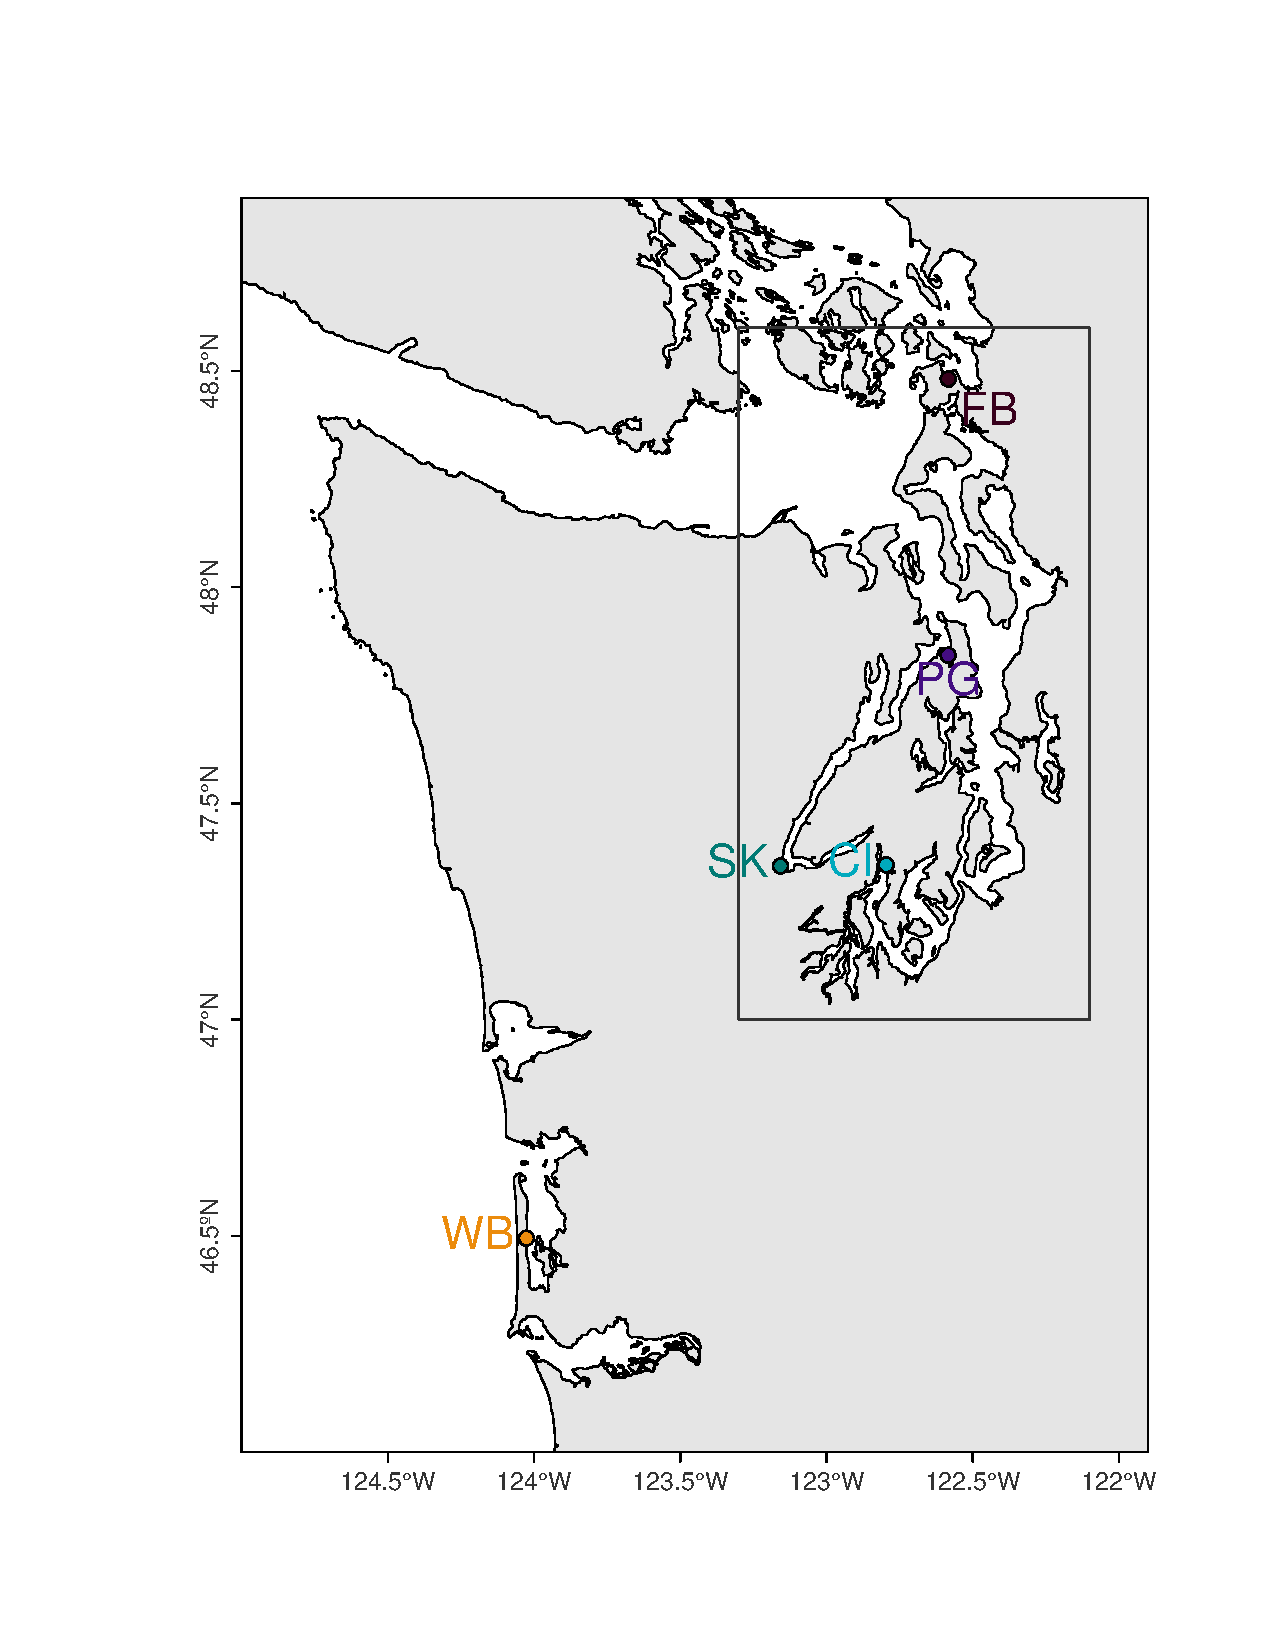
\includegraphics[width=0.65\textwidth]{figure/Ch1/fig1.1.pdf}
  \caption{Map of outplant sites}
  \label{fig:sitemap}
\end{figure}
\clearpage

\textbf{Figure} \ref{fig:envdatalines}: Environmental variables for each site (Case Inlet, Fidalgo Bay, Port Gamble Bay, Skokomish River Delta, and Willapa Bay) and habitat (unvegetated and eelgrass) over the course of the 29 day outplant.\newline
\begin{figure}[h]
\centering
  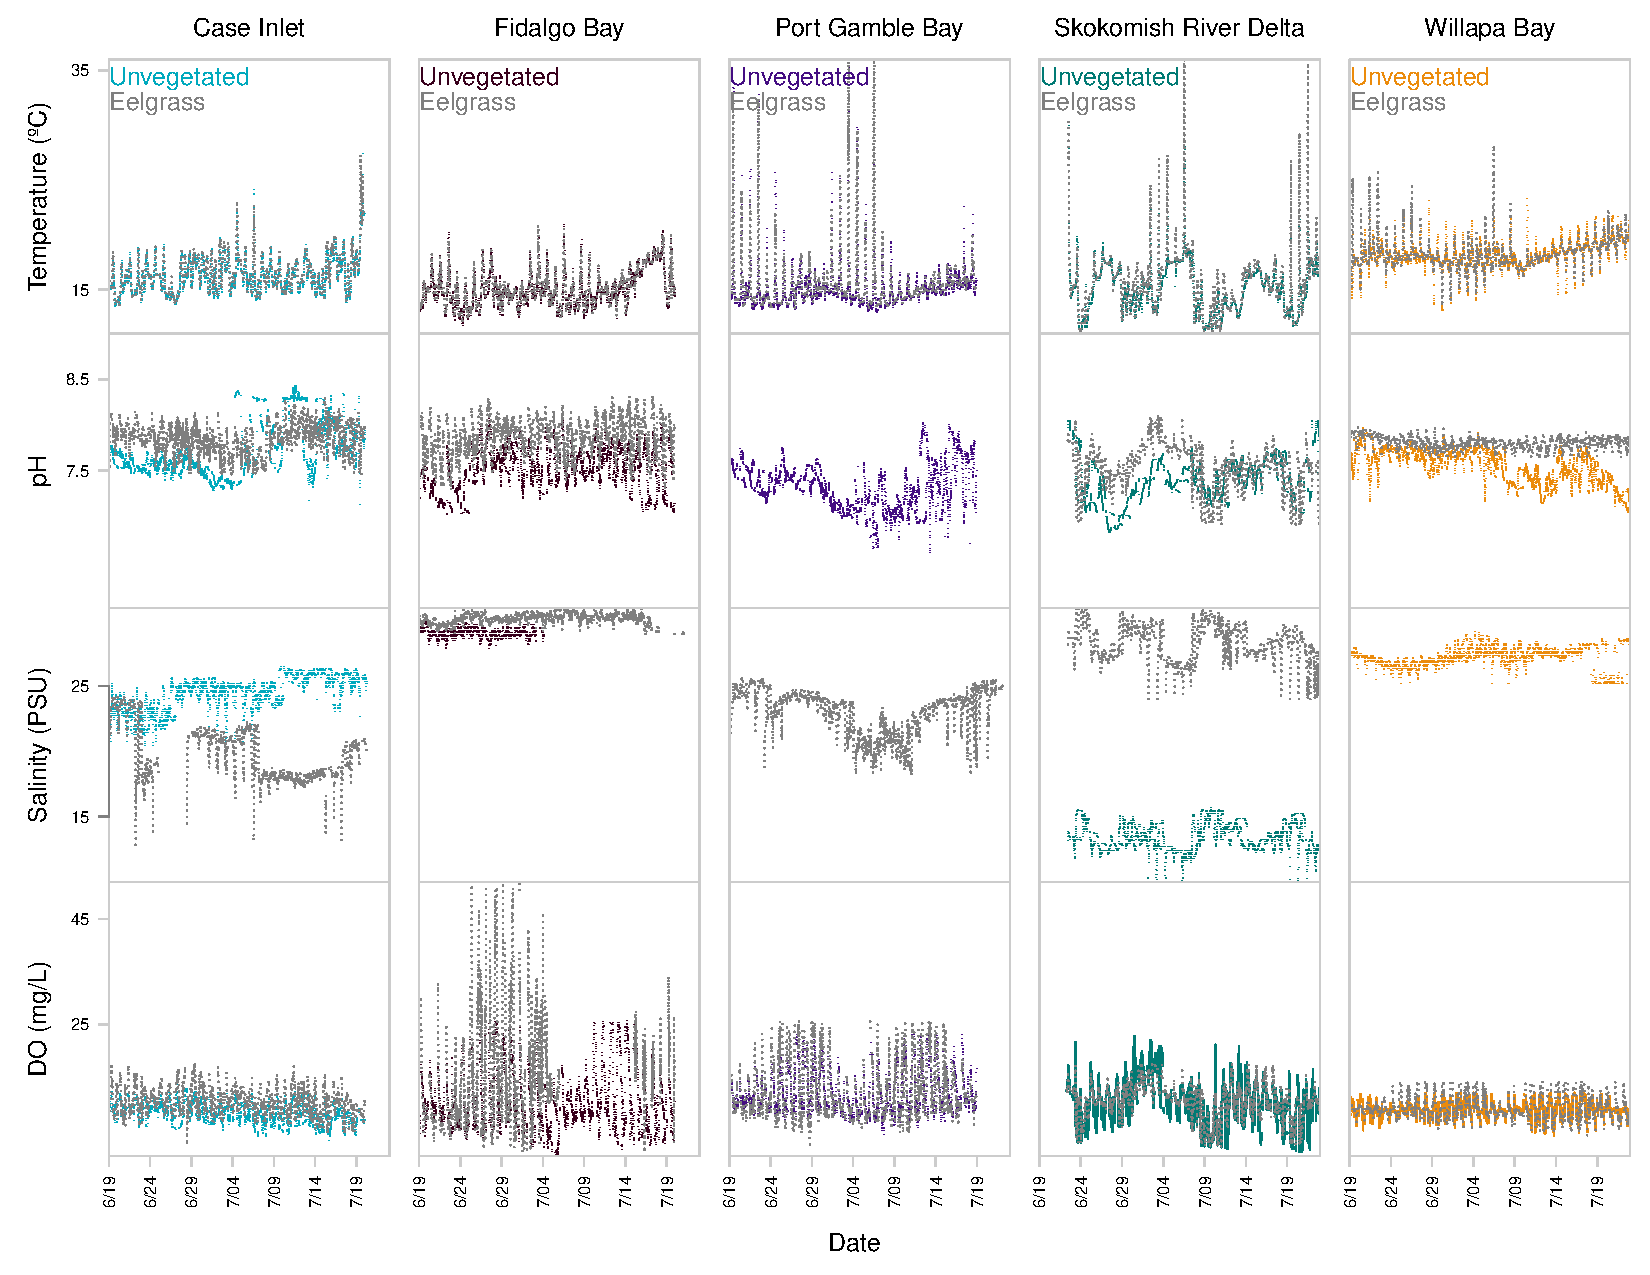
\includegraphics[width=1\textwidth]{figure/Ch1/fig1.2.pdf}
  \caption{Environmental data at each site}
  \label{fig:envdatalines}
\end{figure}
\clearpage

\textbf{Figure} \ref{fig:pepordination}: Ordination results for peptide abundance and environmental data. a) Environmental variables (pH, dissolved oxygen, salinity, and temperature) explained 30\% of variance in peptide abundance data; however, redundancy analysis (RDA) for peptide abundance constrained by environmental variable was not significant (ANOVA; F\textsubscript{6,19} = 1.306, p = 0.195). Temperature mean and variance were the most influential, yet nonsignificant, environmental predictors (ANOVA; temperature mean: F\textsubscript{1,25} = 2.3275, p = 0.065; temperature variance: F\textsubscript{1,25} = 2.1527, p = 0.067). Peptides differentially abundant between Fidalgo Bay (FB) and Willapa Bay (WB) are primarily positively loaded onto temperature mean, with two negatively loaded on temperature variance. b) Non-metric multidimensional scaling plot depicting peptide abundance by site and habitat, with 95\% confidence ellipses around each site (stress = 0.075, p = 0.0099). c) Peptides that contributed to significant peptide abundance differences between FB and WB, as determined by post-hoc similarity percentage analysis (SIMPER). Peptides denoted 1 correspond to peroxiredoxin-5 (PRX), 2 for carbonic anhydrase (CA), 3 for catalase (CAT), 4 for glucose-6-phosphate 1-dehydrogenase (G6PD), 5 for NADP transhydrogenase (NADPt), and 6 for protein disulfide isomerases 1 and 2 (PDI). FB peptide composition was differentiated by CA abundance, while all other proteins influenced peptide abundances at WB.\newline
\begin{figure}[h]
\centering
  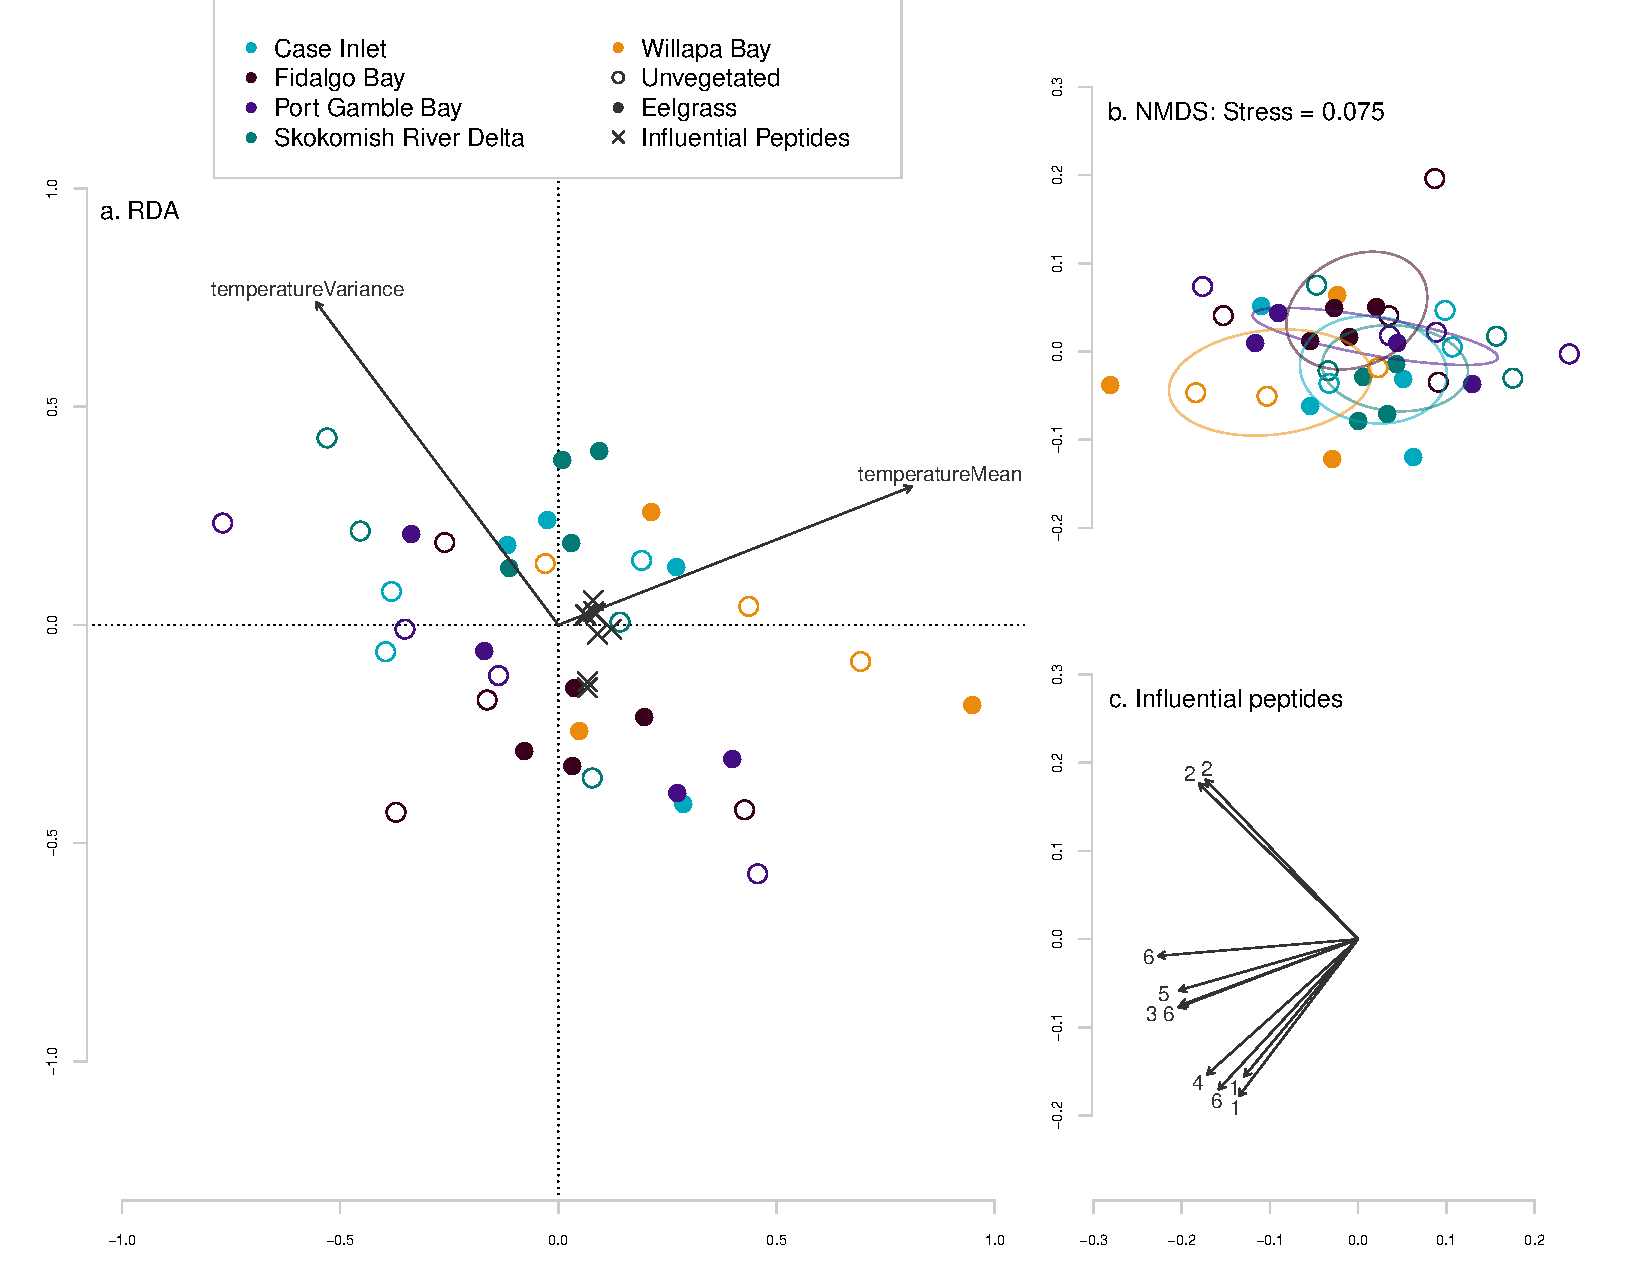
\includegraphics[width=1\textwidth]{figure/Ch1/fig1.3.pdf}
  \caption{Peptide abundance ordination results}
  \label{fig:pepordination}
\end{figure}
\clearpage

\textbf{Figure} \ref{fig:protheatmap}: Average protein abundance by constituent peptides across experimental sites from SRM. Peptide abundance data at each site was averaged, then log transformed. Proteins were considered differentially abundant if at least one constituent peptide was significantly different (indicated by an asterisk). There were no significant differences in protein abundance among the Puget Sound locations, or between unvegetated and eelgrass habitats. Proteins were only significantly different between Fidalgo Bay and Willapa Bay or Skokomish River Delta and Willapa Bay.\newline
\begin{figure}[h]
\centering
  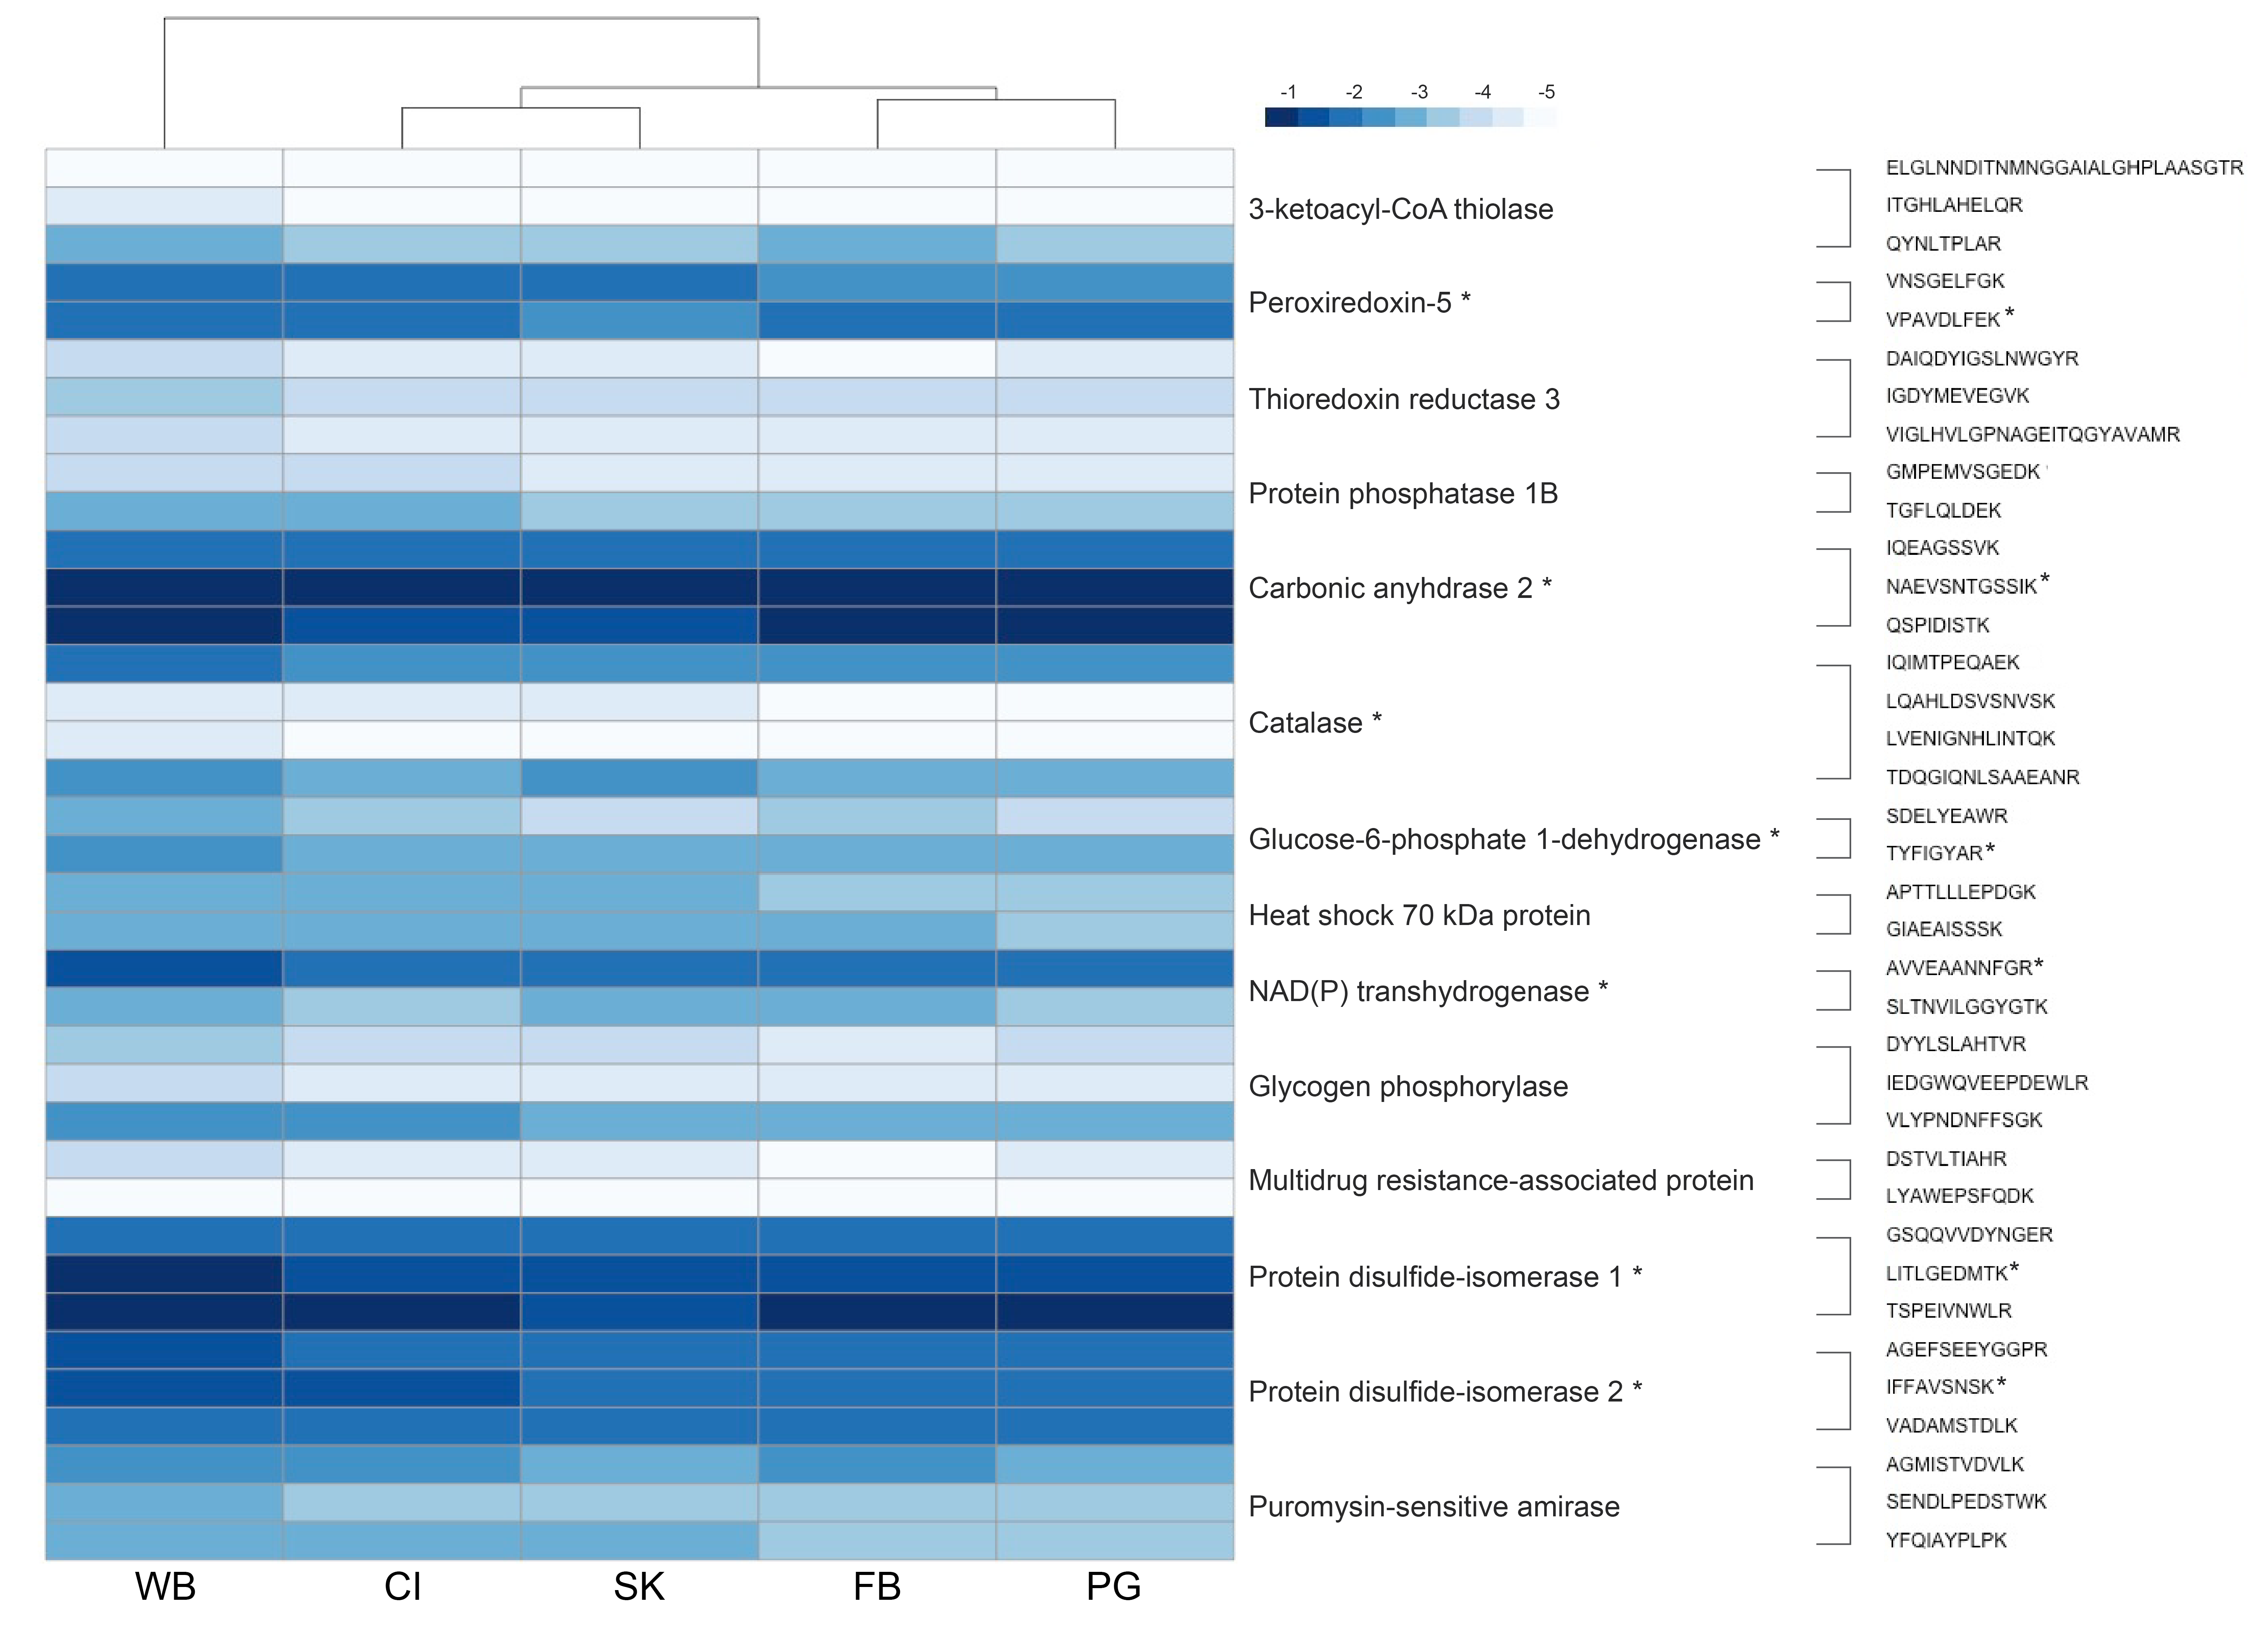
\includegraphics[width=1\textwidth]{figure/Ch1/fig1.4.png}
  \caption{Average protein abundance by site}
  \label{fig:protheatmap}
\end{figure}
\hypertarget{larval-response-to-parental-low-ph-exposure-in-pacific-oysters-crassostrea-gigas}{%
\chapter{\texorpdfstring{Larval response to parental low pH exposure in Pacific oysters (\emph{Crassostrea gigas})}{Larval response to parental low pH exposure in Pacific oysters (Crassostrea gigas)}}\label{larval-response-to-parental-low-ph-exposure-in-pacific-oysters-crassostrea-gigas}}

A version of this chapter was published as: Venkataraman, Y. R., Spencer, L. H., \& Roberts, S. B. (2019). Larval Response to Parental Low pH Exposure in the Pacific Oyster (\emph{Crassostrea gigas}). \emph{Journal of Shellfish Research}, \emph{38(3)}, 743. \url{https://doi.org/10.2983/035.038.0325}

\hypertarget{abstract-1}{%
\section{Abstract}\label{abstract-1}}

As negative effects of ocean acidification are experienced by coastal ecosystems, there is a growing trend to investigate the effect ocean acidification has on multiple generations. Parental exposure to ocean acidification has been shown to induce larval carryover effects, but whether or not acute exposure to a stressor as an adult can influence the larval generation long after the stress has been removed has yet to be tested. To assess how a temporary exposure to experimental ocean acidification affects the ecologically and commercially relevant Pacific oyster (\emph{Crassostrea gigas}), adult oysters were exposed to either low pH (7.31 ± 0.02) or ambient pH (7.82 ± 0.02) conditions for seven weeks. Oysters were then held for eight weeks in ambient conditions, and subsequently reproductively conditioned for four weeks at ambient pH. After conditioning, oysters were strip-spawned to create four families based on maternal and paternal ocean acidification exposure. The number of D-hinge larvae were counted eighteen hours post-fertilization. A sex-specific broodstock response was observed, where female exposure to low pH conditions resulted in fewer D-hinge larvae. This study demonstrates that the effects of ocean acidification can last beyond the time from when the environmental perturbation is experienced. Broadening the understanding of environmental memory will be valuable when considering organismal ability to persist in the face of environmental change.

\hypertarget{introduction-2}{%
\section{Introduction}\label{introduction-2}}

Determining how parental exposure to ocean acidification carries over into early larval stages is important for understanding cumulative effects of climate-related environmental change. Gametogenesis is a key period during which parental exposure to ocean acidification can influence offspring (\protect\hyperlink{ref-Donelson2018}{Donelson, Salinas, Munday, \& Shama, 2018}). Several studies exposing Sydney rock oysters (\emph{Saccostrea glomerata}) to high pCO\textsubscript{2} conditions (856 µatm, pHNBS 7.89-7.90) during reproductive conditioning identified positive larval carryover effects (\protect\hyperlink{ref-Parker2012}{Parker et al., 2012}, \protect\hyperlink{ref-Parker2017}{2017}; \protect\hyperlink{ref-Parker2015}{Parker, O'Connor, Raftos, Pörtner, \& Ross, 2015}). Specifically, larvae from parents exposed to low pH conditions were larger and developed faster in acidified conditions compared to those from parents reared in ambient pH conditions (\protect\hyperlink{ref-Parker2012}{Parker et al., 2012}, \protect\hyperlink{ref-Parker2017}{2017}; \protect\hyperlink{ref-Parker2015}{Parker, O'Connor, Raftos, Pörtner, \& Ross, 2015}). Conversely, similar experiments conducted with northern quahog (= hard clam; \emph{Mercenaria mercenaria}) and bay scallops (\emph{Argopecten irradians}) demonstrated negative larval carryover effects (\protect\hyperlink{ref-Griffith2017}{Griffith \& Gobler, 2017}). Larvae from adult \emph{A. irradians} and \emph{M. mercenaria} exposed to low pH were more sensitive to acidified conditions than those spawned from parents exposed to ambient pH during reproductive conditioning (\protect\hyperlink{ref-Griffith2017}{Griffith \& Gobler, 2017}). These studies demonstrate the importance of parental exposure during reproductive conditioning (late-stage gametogenesis) on offspring.

As the Pacific oyster (\emph{Crassostrea gigas}; Thunberg, 1793) is a commercially and ecologically relevant species in much of the world, several research efforts have identified consequences of ocean acidification for distinct \emph{C. gigas} life stages. While fertilization still occurs under near-future ocean acidification conditions (\protect\hyperlink{ref-Boulais2018}{Boulais et al., 2018}; \protect\hyperlink{ref-Havenhand2009}{Havenhand \& Schlegel, 2009}; \protect\hyperlink{ref-Kurihara2007}{Kurihara, Kato, \& Ishimatsu, 2007}), fertilization success in acidified conditions is variable between \emph{C. gigas} populations (\protect\hyperlink{ref-Barros2013}{Barros, Sobral, Range, Chı́charo, \& Matias, 2013}; \protect\hyperlink{ref-Parker2010}{Parker, Ross, \& O'Connor, 2010}). Researchers have found that larvae experience developmental delays and reduced shell growth when exposed to experimental ocean acidification conditions (\protect\hyperlink{ref-Gazeau2011}{Gazeau et al., 2011}; \protect\hyperlink{ref-Kurihara2007}{Kurihara, Kato, \& Ishimatsu, 2007}; \protect\hyperlink{ref-Timmins-Schiffman2013}{E. Timmins-Schiffman, O'Donnell, Friedman, \& Roberts, 2013}; \protect\hyperlink{ref-Waldbusser2014}{Waldbusser et al., 2014}). Natural upwelling-induced ocean acidification conditions also reduced larval production and growth in a hatchery setting (\protect\hyperlink{ref-Barton2012}{Barton, Hales, Waldbusser, Langdon, \& Feely, 2012}). Ocean acidification hampers protein expression in larvae, especially for proteins related to calcification and cytoskeleton production (\protect\hyperlink{ref-Dineshram2012}{R. Dineshram et al., 2012}). During metamorphosis, oyster larvae experience down-regulation of proteins related to energy production, metabolism, and protein synthesis (\protect\hyperlink{ref-Dineshram2016}{Ramadoss Dineshram et al., 2016}). Adult \emph{C. gigas} calcification rates decrease as seawater pCO\textsubscript{2} increases (\protect\hyperlink{ref-Gazeau2007}{Gazeau et al., 2007}), with oysters grown at 2800 µatm displaying significantly lower fracture toughness than oyster shells from ambient conditions (\protect\hyperlink{ref-Timmins-Schiffman2014}{E. Timmins-Schiffman et al., 2014}). Exposure to ocean acidification also affects adult antioxidant responses, carbohydrate metabolism, transcription, and translation protein pathways (\protect\hyperlink{ref-Timmins-Schiffman2014}{E. Timmins-Schiffman et al., 2014}). Predator-prey interactions can also change under experimental ocean acidification (\protect\hyperlink{ref-Wright2018}{Wright, Parker, O'Connor, Scanes, \& Ross, 2018}). There is limited evidence, however, of how ocean acidification influences Pacific oysters across multiple generations.

The current study is the first to discern how exposure to experimental ocean acidification prior to reproductive conditioning affects larval abundance in \emph{C. gigas}. This experiment not only describes how isolated exposure to low pH during early gametogenesis influences larvae, but also provides information on the effects of acute pH exposure on adult gonad morphology. Additionally, the study demonstrates how environmental perturbation experienced before reproductive maturity affects the subsequent generation, even if the stressor is long-removed.

\hypertarget{methods-1}{%
\section{Methods}\label{methods-1}}

\hypertarget{experimental-overview}{%
\subsection{Experimental overview}\label{experimental-overview}}

Experimental trials were conducted at the Kenneth K. Chew Center for Shellfish Research and Restoration at the National Oceanic and Atmospheric Administration (NOAA) Manchester Field Station (47°34'09.1``N 122°33'19.0''W, Manchester, Washington, USA) in 2017. Adult hatchery-raised \emph{C. gigas} (average shell length = 117.46 ± 19.16 cm) were acclimated in the facility for 10 days, then exposed to either low or ambient pH conditions for 48 days (Figure 2.1). After pH exposure, oysters were held at ambient pH and water temperature conditions for 90 days. Oysters underwent reproductive conditioning for 22 days, then strip-spawned. D-hinge larvae were counted eighteen hours after fertilization occurred.

\hypertarget{experimental-ph-exposure}{%
\subsection{Experimental pH exposure}\label{experimental-ph-exposure}}

The experimental system consisted of a 1,610 liter storage tank that fed two 757 liter header tanks. Water from Clam Bay, WA was pumped through a sand filter, then UV-treated. The UV-treated water passed through a set of three sock filters (100 µm, 50 µm, and 25 µm) and a degassing column. Once degassed, water passed through three more sock filters (25 µm, then 10 µm, and 5 µm) before entering the storage tank. The storage tank was outfitted with an off-gas vent and pump to recirculate water such that CO\textsubscript{2} in the water could be equilibrated with atmospheric CO\textsubscript{2}. Equilibrated water flowed into the two header tanks, each of which fed three 50L flow-through (1.2 L/min) experimental tanks (six experimental tanks total). For all header and experimental tanks, pH in header and experimental tanks was continuously monitored using Durafet pH probes (Honeywell Model 51453503-505) and an AVTECH system. The addition of CO\textsubscript{2} in the low pH header tank was controlled using a solenoid valve. A Dual Input Analytical Analyzer (Honeywell Model 50003691-501) automatically mediated solenoid injections. A CO\textsubscript{2} airline with a back pressure of 15 psi, controlled with a regulator, injected CO\textsubscript{2} into the low pH header tank every 180 seconds with an injection duration of 0.4 seconds. Injections only occurred if real-time pH from the Durafet was above pH 7.22. A venturi injector connected to the ambient water line mixed ambient pH water with CO\textsubscript{2}-rich water to lower pH. There were no CO\textsubscript{2} injections in the ambient header tank.

Prior to the pH exposure trial, twenty randomly selected \emph{C. gigas} were lethally sampled to assess gonadal status (see \emph{Histological analysis}). Oysters were placed in each flow-through experimental tank in ambient water conditions and exposed to ambient or low pH conditions for seven weeks. Each treatment consisted of 3 tanks, each with 20 oysters. All experimental tanks received algae from a common reservoir. The algal tank contained 300-500 mL of Shellfish Diet 1800® (Reed Mariculture) diluted in 200L of ambient pH seawater (\protect\hyperlink{ref-Helm2004}{Helm \& Bourne, 2004}). Algae was continuously dosed to oyster experimental tanks using an Iwaki Metering Pump. Algal lines were cleaned twice weekly, and experimental tanks were fully drained and cleaned once a week.

\hypertarget{seawater-chemistry-analysis}{%
\subsection{Seawater chemistry analysis}\label{seawater-chemistry-analysis}}

Twice a week, water samples (1L) were collected from each header and oyster experimental tank. For each sample, salinity was measured with a Bench/Portable Conductivity Meter (Model 23226-505, VWR), pH (mV) was measured with a Combination pH Electrode (Model 11278-220, Mettler Toledo), and temperature (ºC) was measured using a Traceable Digital Thermometer (Model 15-077, Fisher). To calibrate the pH probe, a Tris buffer (0.08 M, 28.0 salinity) was prepared using 0.3603 mol of NaCl (J.T. Baker), 0.0106 mol of KCl (Fisher Scientific), 0.0293 mol MgSO4-(H2O)7 (Fisher Scientific), 0.0107 mol of CaCl2-2(H2O) (MP Biomedicals), 0.0401 HCl (J.T. Baker), and 0.0799 mol of Tris base (Fisher Scientific). Deionized water was added for a final volume of 1L. Salinity, temperature, and pH measurements for the Tris buffer were obtained at five temperatures before measuring samples to generate a standard curve. This standard curve was used to calibrate the pH electrode and convert measured millivolts to pH units.

For total alkalinity measurements, duplicate seawater samples (250 mL) were collected from experimental tanks twice weekly and dosed with mercuric chloride (50 µL of 0.18 M solution) to preserve samples (\protect\hyperlink{ref-Bandstra2006}{Bandstra, Hales, \& Takahashi, 2006}). Samples from days 5, 33, and 48 were run on a T5 Excellence titrator (Mettler Toledo) to determine alkalinity. Salinity from discrete samples was used to calculate total alkalinity, using the \texttt{seacarb} library in R (\protect\hyperlink{ref-Gattuso2018}{Gattuso et al., 2018}). Calculated pH, total alkalinity, temperature, and salinity were also used in \texttt{seacarb} to calculate in situ pH, pCO\textsubscript{2}, dissolved organic carbon (DIC), calcite saturation (Ω\textsubscript{calcite}), and aragonite saturation (Ω\textsubscript{aragonite}) for days 5, 33, and 48. R code used to calculate water chemistry parameters is available in the associated Github repository (Appendix 1).

\hypertarget{histological-analysis}{%
\subsection{Histological analysis}\label{histological-analysis}}

Twenty randomly selected \emph{C. gigas} were lethally sampled before pH exposure for histological analyses. On the last day of low pH exposure, ten oysters from each treatment --- randomly selected from each tank --- were also lethally sampled to assess gonadal status. For each sampled oyster, a piece of gonad tissue was cut and placed in a histology cassette. Gonad tissue in cassettes was fixed for histology using PAXgene Tissue FIX and STABILIZER and sent to Diagnostic Pathology Medical Group, Inc.~(Sacramento, CA) for staining with hematoxylin and eosin and slide preparation. Tissues exposed to ambient pH were confounded during processing, preventing any tank identification. Maturation state and organism sex was evaluated histologically at 40x magnification (\protect\hyperlink{ref-Enriquez-Diaz2008}{Enrı́quez-Dı́az, Pouvreau, Chávez-Villalba, \& Le Pennec, 2008}; \protect\hyperlink{ref-Fabioux2005}{Fabioux, Huvet, Le Souchu, Le Pennec, \& Pouvreau, 2005}).

\hypertarget{reproductive-conditioning}{%
\subsection{Reproductive conditioning}\label{reproductive-conditioning}}

Following seven weeks of low pH exposure, oysters were returned to a common garden and maintained at ambient pH conditions for eight weeks. Afterwards, oysters were reproductively conditioned. Water temperatures and food quantity are known to regulate the timing, speed, and intensity of gametogenesis in \emph{C. gigas} (\protect\hyperlink{ref-Enriquez-Diaz2008}{Enrı́quez-Dı́az, Pouvreau, Chávez-Villalba, \& Le Pennec, 2008}). Conditioning protocol was modeled after standard hatchery practices (Molly Jackson, Broodstock Manager at Taylor Shellfish, pers. comm., June 2017). Water temperature was raised from ambient conditions (13ºC) to 23ºC over three weeks (1ºC/2 days), since optimal temperature for \emph{C. gigas} gametogenesis is between 18ºC and 26ºC (\protect\hyperlink{ref-Parker2010}{Parker, Ross, \& O'Connor, 2010}). Conditions were maintained at 23ºC for one more week prior to spawning. During conditioning, \emph{C. gigas} were fed 700-800 mL of Shellfish Diet 1800® daily (\protect\hyperlink{ref-Helm2004}{Helm \& Bourne, 2004}).

\hypertarget{strip-spawning-and-larval-rearing}{%
\subsection{Strip spawning and larval rearing}\label{strip-spawning-and-larval-rearing}}

After reproductive conditioning, all surviving oysters were prepared for strip spawning. A sample of gonad from each individual was assessed for presence of active sperm or eggs using a microscope at 10x magnification. Only \emph{C. gigas} with active sperm or eggs were used for crosses (n\textasciitilde male, low\textasciitilde{} = 6, n\textasciitilde female, low\textasciitilde{} = 22, n\textasciitilde male, ambient\textasciitilde{} = 6, n\textasciitilde female, ambient\textasciitilde{} = 26). Presence of mature gametes and ripe oysters indicated that oysters were in good condition and not affected by use of Shellfish Diet 1800® instead of live algae during reproductive conditioning. For each treatment (low pH and ambient conditions), one gram of mature gonad from each ripe female was pooled. The number of eggs in both the ambient and low pH pools were counted to determine the number of eggs used for parental crosses. Parental crosses were created using 210,000 eggs from the female egg pools and sperm (200 µL) from individual males.

Four half-sibling families were created based on parental pH exposure: low pH female (pool) x low pH male, low pH female (pool) x ambient pH male, ambient pH female (pool) x low pH male, and ambient pH (pool) female x ambient pH male. These crosses were conducted using pooled eggs from either low pH or ambient pH females, and sperm from one of six males within each pH treatment (e.g.~low pH female pool x low pH male-01, low pH female pool x low pH male-02, \ldots{} low pH female pool x low pH male-06), totaling 24 crosses. All crosses were performed in duplicate, resulting in 48 separate fertilization events.

Fertilization was carried out in plastic beakers (1L) for 20 minutes with static 23ºC filtered seawater (1 µm) in ambient pH conditions. After confirming polar body formation, beaker contents were transferred to larger plastic tanks (19L) with aerated, static 23ºC filtered seawater (1 µm) for eighteen hours of incubation. Duplicate containers were combined eighteen hours post-fertilization, and D-hinge larvae were counted for each cross (n= 24).

\hypertarget{statistical-analyses}{%
\subsection{Statistical analyses}\label{statistical-analyses}}

Differences in in situ pH, total alkalinity, pCO\textsubscript{2}, DIC, Ω\textsubscript{calcite}, and Ω\textsubscript{aragonite} between pH treatments were evaluated with a one-way ANOVA. Because tissue samples were confounded during histological processing, a binomial GLM model was used to compare gonad maturation between pH treatments. Differences in sex ratios between pH treatments were evaluated using a chi-squared test of homogeneity. To identify differences in D-hinge larval counts, a linear mixed model was used, with sire and female egg pool as random effects. Differences in D-hinge larval counts by female treatment were assessed using a similar linear mixed model, with only sire as a random effect. Normality of data, as well as independence and homoscedasticity, were verified visually. All statistical analyses were carried out in R (Version 3.4.0). R Scripts are available in the associated Github repository (Appendix 1).

\hypertarget{results-1}{%
\section{Results}\label{results-1}}

\hypertarget{water-chemistry}{%
\subsection{Water chemistry}\label{water-chemistry}}

Pacific oysters exposed to low pH experienced different water chemistry parameters than those in the ambient pH treatment (Table 2.1). Using water samples from days 5, 33, and 48, pH (One-way ANOVA; F\(_{1,16}\) = 5838.7810, p = 6.1165e-22), pCO\textsubscript{2} (One-way ANOVA; F\(_{1,16}\) = 235.4018, p = 5.4421e-11), DIC (One-way ANOVA; F\(_{1,16}\) = 7.1222, p = 0.0168), Ω\textsubscript{calcite} (One-way ANOVA; F\(_{1,16}\) = 528.9468, p = 1.0989e-13), Ω\textsubscript{aragonite} (One-way ANOVA; F\(_{1,16}\) = 526.5207, p =1.1389e-13) were significantly lower in the low pH treatment. Total alkalinity, however, was not significantly different between pH treatments (One-way ANOVA; F\(_{1,16}\) = 1.382, p = 0.2570).

\hypertarget{gonad-maturation}{%
\subsection{Gonad maturation}\label{gonad-maturation}}

A binomial GLM was used to compare gonad maturation of individuals sampled before and immediately after pH exposure, but before reproductive conditioning. The most parsimonious model included only sampling time (before or after pH treatment). Gonad maturation status was not significantly different between \emph{C. gigas} sampled before and after pH treatment (binomial GLM; F\(_{2,37}\) = 0.7973, p = 0.3442). Additionally, maturation status was not different between pH treatments (binomial GLM; F\(_{3,36}\) = 2.2675, p = 0.1408). No sampled oysters possessed fully mature gametes, but some males sampled appeared to be undergoing resorption (Appendix 1). Sex ratios were also similar between low and ambient pH treatments (Chi-squared test for homogeneity; X\textsuperscript{2}\textsubscript{2} = 3.2279; p = 0.1942).

\hypertarget{larval-survival}{%
\subsection{Larval Survival}\label{larval-survival}}

A linear mixed effect model, with female pool and sire as random effects, demonstrated no significant difference in the number of D-hinge larvae counted eighteen hours post-fertilization between all four parental families (Linear mixed effect model; X\textsuperscript{2}\textsubscript{3} = 3.1325; p = 0.1066). Sire and female egg pools accounted for 0.8530\% and 3.1623\% of total variance, respectively. Significantly fewer D-hinge larvae were present in half-sibling families where females were exposed to low pH conditions (Figure \ref{fig:carryoverboxplot}; Linear mixed effect model; X\textsuperscript{2}\textsubscript{1} = 8.1781; p = 0.0042), with sire accounting for 0.3116053\% of total variance.

\hypertarget{discussion-1}{%
\section{Discussion}\label{discussion-1}}

The present study is the first to document the transgenerational influence of ocean acidification on Pacific oysters. Larval \emph{C. gigas} was negatively impacted when maternal broodstock were exposed to low pH (pH = 7.31), suggesting a maternal carryover effect. The experimental design of this study is also unique --- adult \emph{C. gigas} experienced low pH conditions three months prior to reproductive conditioning, then were kept solely in ambient pH conditions through strip spawning and larval rearing. Since environmental perturbation experienced before Pacific oysters were mature still affected larval oysters, the results indicate a role for environmental memory in \emph{C. gigas} response to ocean acidification. Mechanisms for transgenerational environmental memory have been explored in response to acute stressors in other species. For example, \emph{Daphnia magna} exposed to high salinity conditions had altered DNA methylation patterns, and these patterns were inherited by the following three non-exposed generations (\protect\hyperlink{ref-Jeremias2018}{Jeremias et al., 2018}). Significant carryover effects observed in \emph{C. gigas} --- solely exposed to low pH when immature --- broaden the current understanding of stressor timing and its effect on organismal physiology.

While it is evident that acute exposure to low pH experienced by adult \emph{C. gigas} resulted in detrimental effects for larvae, the fact that larvae were not reared in acidified conditions makes cross-study comparison difficult. If \emph{C. gigas} larvae were also reared in acidified conditions, it is possible that larvae with a history of parental exposure to experimental ocean acidification may have exhibited a negative carryover effect on larval growth and performance. Negative carryover effects have been found in other marine invertebrate taxa, but all studies involved exposure to experimental ocean acidification during reproductive conditioning and larval rearing in acidified conditions. Tanner crabs (\emph{Chionoecetes bairdi}) solely exposed to acidified water (pH 7.5 or 7.8) as larvae did not exhibit significant changes in morphology, size, Ca/Mg content, or metabolic rate, yet substantial effects on physiology was observed when larvae had a history of maternal exposure during oogenesis (\protect\hyperlink{ref-Long2016}{Long, Swiney, \& Foy, 2016}). Larvae from adult northern quahog (= hard clam; \emph{M. mercenaria}) and bay scallops (\emph{A. irradians}) developed slower when parents were reproductively conditioned in low pH conditions (pH\textsubscript{T} = 7.4) (\protect\hyperlink{ref-Griffith2017}{Griffith \& Gobler, 2017}). Additionally, larvae with a history of parental low pH exposure were more vulnerable to additional stressors like thermal stress, limited food, and harmful algae exposure (\protect\hyperlink{ref-Griffith2017}{Griffith \& Gobler, 2017}). Although \emph{C. gigas} were not reproductively conditioned in acidified water, and the present study cannot distinguish between hatching success and early mortality, identifying a similar negative larval carryover effect four months after an acute environmental perturbation is arguably more surprising and significant, particularly in terms of efforts to understand the mechanism of environmental memory.

The severity of conditions experienced by organisms may also explain whether or not offspring demonstrate transgenerational acclimatization to stressors. For example, the negative carryover effect observed in \emph{C. gigas} is different from the positive carryover effects observed in ocean acidification experiments conducted with Sydney rock oysters. When adult \emph{S. glomerata} were exposed to acidified seawater (pCO\textsubscript{2} = 856 µatm; pH\textsubscript{NBS} = 7.89-7.90) during reproductive conditioning, resultant larvae were larger and developed faster in acidified conditions when compared to larvae from parents exposed to ambient conditions (\protect\hyperlink{ref-Parker2012}{Parker et al., 2012}). This positive carryover effect was found to persist in the F2 generation. In acidified conditions, F2 offspring with a history of transgenerational (F0 and F1) pCO\textsubscript{2} exposure grew faster and demonstrated fewer shell abnormalities (\protect\hyperlink{ref-Parker2015}{Parker, O'Connor, Raftos, Pörtner, \& Ross, 2015}). While species-specific responses can certainly explain the observed differences in larval phenotypes, it is also likely that inconsistencies in treatment conditions between experiments resulted in dose-dependent effects. \protect\hyperlink{ref-Parker2012}{Parker et al.} (\protect\hyperlink{ref-Parker2012}{2012}), \protect\hyperlink{ref-Parker2015}{Parker, O'Connor, Raftos, Pörtner, \& Ross} (\protect\hyperlink{ref-Parker2015}{2015}), and \protect\hyperlink{ref-Parker2017}{Parker et al.} (\protect\hyperlink{ref-Parker2017}{2017}) used a high pCO\textsubscript{2} treatment of 856 µatm (pH = 7.89-7.90), with a control of 380-385 µatm (pH = 8.19-8.20). Therefore, the elevated pCO\textsubscript{2} treatment used in those studies is similar to the ambient pH treatment (7.82; pCO\textsubscript{2} = 747.51-912.22) in the present study. Sydney rock oyster larvae with a history of transgenerational exposure exhibited faster development, but exhibited similar survival and were only 10\% larger in acidified conditions when compared to larvae with no transgenerational exposure history (\protect\hyperlink{ref-Parker2012}{Parker et al., 2012}). With a relatively smaller effect size and a milder treatment than used in this study, it is possible these studies are not at odds but reflect dose-dependent effects on larval phenotypes. Negative carryover effects demonstrated in this study and in \protect\hyperlink{ref-Griffith2017}{Griffith \& Gobler} (\protect\hyperlink{ref-Griffith2017}{2017}) can also be attributed to similar treatment pH levels {[}\protect\hyperlink{ref-Griffith2017}{Griffith \& Gobler} (\protect\hyperlink{ref-Griffith2017}{2017}): pHT = 7.4; this study: pH = 7.31{]}. Both of these studies used treatment levels more extreme than International Panel on Climate Change projections for open ocean acidification, but consistent with coastal and estuarine acidification scenarios experienced at study locations (\protect\hyperlink{ref-Feely2010}{Feely et al., 2010}; \protect\hyperlink{ref-Griffith2017}{Griffith \& Gobler, 2017}; \protect\hyperlink{ref-Pelletier2018}{Pelletier, Roberts, Keyzers, \& Alin, 2018}). More research is required to understand how location-specific conditions will affect multiple generations in a single species.

Although the effect of water chemistry on gametogenesis has been recorded in other taxa, it is unlikely that a low pH exposure occurring three months prior to reproductive conditioning could have affected gonad maturation. Studies in which reproductive conditioning and experimental ocean acidification occur concurrently have demonstrated negative effects on maturation and fecundity. Gametogenesis, especially oogenesis, was disrupted in eastern oysters (\emph{Crassostrea virginica}) that experienced severe ocean acidification conditions during reproductive conditioning (pH = 7.71, 5584 µatm) (\protect\hyperlink{ref-Boulais2017}{Boulais et al., 2017}). Green sea urchins (\emph{Stronglyocentrotus droebachiensis}) exposed to high pCO\textsubscript{2} (1200 µatm) conditions for four months demonstrated low fecundity (\protect\hyperlink{ref-Dupont2013}{Dupont, Dorey, Stumpp, Melzner, \& Thorndyke, 2013}), and \emph{S. glomerata} conditioned in high pCO\textsubscript{2} (856 µatm) conditions exhibited reduced rates of gametogenesis, smaller gonad area, and reduced fecundity (\protect\hyperlink{ref-Parker2018}{Parker et al., 2018}). Gonad histology from \emph{C. gigas} taken immediately after low or ambient pH exposure did not indicate any differences in maturation state, or interaction between sex and maturation state, between treatments. Even if fecundity or rates of gametogenesis differed between treatments, a return to ambient conditions for three months may have reversed any detrimental effects.

Reduced \emph{C. gigas} larval abundance could have been a result of altered maternal provisioning in female oysters exposed to low pH conditions. In the face of stressors, females can either increase maternal provisioning (\protect\hyperlink{ref-Allen2008}{Allen, Buckley, \& Marshall, 2008}; \protect\hyperlink{ref-Sunday2011}{Sunday, Crim, Harley, \& Hart, 2011}) --- diverting more resources, like lipids or proteins, into eggs --- or decrease provisioning due to energetic constraints (\protect\hyperlink{ref-Liu2010}{W. Liu, Li, Gao, \& Kong, 2010}; \protect\hyperlink{ref-Uthicke2013}{Uthicke, Soars, Foo, \& Byrne, 2013}). For example, changes in fatty acid provisioning from maternal exposure to high pCO\textsubscript{2} conditions (2300 µatm) in Atlantic silverside (\emph{Menidia menidia}) resulted in lower embryo survival when eggs lacked certain fatty acids (\protect\hyperlink{ref-Snyder2018}{Snyder, Murray, \& Baumann, 2018}). This phenomenon, however, was not documented in the Sydney rock oyster: while elevated pCO\textsubscript{2} conditions (856 µatm) reduced the amount of energy invested in maternal gonads, these conditions did not impact \emph{S. glomerata} egg size or total lipid content (\protect\hyperlink{ref-Parker2018}{Parker et al., 2018}). Since adult \emph{C. gigas} did not experience environmental perturbation after low pH exposure, and received enough food to spawn well, any impact on maternal provisioning and subsequent larval abundance was likely a result of low pH three months prior to reproductive conditioning.

The documented effect on Pacific oyster larval abundance four months after low pH exposure indicates an important role for environmental memory in \emph{C. gigas} response to ocean acidification. Low pH exposure may have induced epigenetic modifications (eg. changes in DNA methylation) in adult \emph{C. gigas}. Studies of finfish and shellfish aquaculture species have demonstrated environmentally-induced epigenetic modifications that modify phenotypic responses in organisms (\protect\hyperlink{ref-Gavery2017}{Gavery \& Roberts, 2017}). One notable study on \emph{C. gigas} examined parental effects of adult pollutant exposure on offspring (\protect\hyperlink{ref-Rondon2017}{Rondon et al., 2017}). Spat from parents exposed to the herbicide diuron had differential methylation in coding regions, with some changes leading to differential gene expression (\protect\hyperlink{ref-Rondon2017}{Rondon et al., 2017}). This research indicates that a mechanism crucial for phenotypic plasticity and acclimation across generations exists, and this knowledge can be analyzed in the context of climate-related environmental stressors. Epigenetic modifications in response to ocean acidification have been documented in coral species (\protect\hyperlink{ref-Putnam2016}{Putnam, Davidson, \& Gates, 2016}), but not in molluscs. Several experimental ocean acidification studies, however, hint at the role of epigenetic memory. Olympia oysters (\emph{Ostrea lurida}) exposed to high pCO\textsubscript{2} (1000 µatm) conditions still grew less in the juvenile life stage than counterparts reared in ambient pCO\textsubscript{2}, even after the stressor had been removed (\protect\hyperlink{ref-Hettinger2013}{Hettinger et al., 2013}). Similarly, transgenerational acclimation of \emph{S. glomerata} larvae with a history of exposure to acidified conditions could be explained by changes in epigenome that affect organismal performance (\protect\hyperlink{ref-Parker2012}{Parker et al., 2012}, \protect\hyperlink{ref-Parker2017}{2017}; \protect\hyperlink{ref-Parker2015}{Parker, O'Connor, Raftos, Pörtner, \& Ross, 2015}). Methylation levels are known to increase over the course of gametogenesis, with male and female \emph{C. gigas} exhibiting significantly different methylation patterns (\protect\hyperlink{ref-Zhang2018}{X. Zhang, Li, Kong, \& Yu, 2018}). If epigenetic modifications were acquired by female oysters during low pH exposure, it could explain why a significant effect on larval abundance was detected four months after the exposure ended. Epigenetic mechanisms and altered maternal provisioning are not necessarily mutually exclusive --- changes in the methylome could influence maternal provisioning --- and both could contribute to the results observed in this study.

The results of this study emphasize the need to broaden the scope of when environmental perturbation experienced by an organism is considered stressful, and when an effect can be detected. Although there was no observable effect on adult gonad maturation right after low pH exposure, significant differences in larval abundance were detected four months after the exposure ended. Stressor timing and duration can impact transgenerational responses between mature parents and offspring (\protect\hyperlink{ref-Donelson2018}{Donelson, Salinas, Munday, \& Shama, 2018}). While experimental ocean acidification (pH 7.7; pCO\textsubscript{2} = 800 µatm) increased female investment in amphipods (\emph{Gammarus locusta}), the subsequent generation exhibited fewer eggs and lower fecundity in the same conditions (\protect\hyperlink{ref-Borges2018}{Borges, Figueiredo, Sampaio, Rosa, \& Grilo, 2018}). Transgenerational benefits of maternal exposure to different temperatures (17ºC or 21ºC) in threespine stickleback (\emph{Gasterosteus aculeatus}) differed based on exposure duration (\protect\hyperlink{ref-Shama2014}{Shama \& Wegner, 2014}). Grandparents (F0) were only exposed to treatment temperatures during reproductive conditioning, while parents (F1) experienced either temperature over the course of development. The F1 generation exhibited temperature tolerances similar to the F0 maternal rearing environment, but the F2 generation tolerance was more similar to the F0 generation than the F1 generation (\protect\hyperlink{ref-Shama2014}{Shama \& Wegner, 2014}). The present study demonstrates that length and timing of environmental perturbation experienced by immature individuals can still affect offspring. \protect\hyperlink{ref-Massamba-NSiala2014}{Massamba-N'Siala, Prevedelli, \& Simonini} (\protect\hyperlink{ref-Massamba-NSiala2014}{2014}) elucidated a similar phenomenon with marine polychaetes (\emph{Ophryotocha labronica}): offspring experienced positive carryover effects of female exposure to temperature conditioning only when mothers were exposed to these conditions during late oogenesis; exposure during early oogenesis lead to negative carryover effects. More research should be conducted to understand how stressor timing, specifically before reproductive maturity, can impact carryover effects.

Most other experiments investigating stressor timing are conducted in a multiple stressor framework (\protect\hyperlink{ref-Gunderson2016}{Gunderson, Armstrong, \& Stillman, 2016}). For example, elevated temperatures and low salinity had synergistic effects on \emph{O. lurida} when they were co-occurring stressors, but two to four weeks of recovery in between stressors negated these effects (\protect\hyperlink{ref-Bible2017}{Bible et al., 2017}). Incorporating recovery time in a single-stressor experimental design is also crucial for accurately understanding how environmental perturbation impacts organism physiology. Exposure at one point in time may elicit a response much later in time, in a different environmental setting, or in a different generation, as evidenced by the present study and \protect\hyperlink{ref-Hettinger2013}{Hettinger et al.} (\protect\hyperlink{ref-Hettinger2013}{2013}). The experimental design in the present study is unique, featuring a significant recovery time between low pH exposure and spawning. More single-stressor experiments should incorporate lag times between exposure to stress and measuring response variables to understand if these responses change over time. Adding a multigenerational component to such experiments can elucidate if acute exposures generate carryover effects.

Significant decreases in larval abundance four months after broodstock were exposed to acidified seawater has implications for both aquaculture and natural \emph{C. gigas} populations. Parents and offspring --- or even different offspring life stages --- may not experience the same environmental chemistry. For example, upwelling conditions affecting adult \emph{C. gigas} may subside once spawning occurs. Long-term monitoring of wild Pacific oyster populations, with detailed environmental chemistry reporting, will be crucial for understanding how brief exposures to adverse conditions affect reproductive success and larval abundance in the field. Responses to stressors should not only be documented during and after the perturbation occurs, but also for an extended time afterward. Hatchery-reared \emph{C. gigas} larvae can also experience different conditions than broodstock. Facilities unable to control water chemistry conditions may be exposing immature individuals to environmental perturbations that could affect larvae once spawned. The success of ``priming'' --- exposing \emph{C. gigas} to stressful conditions to induce environmental memory and increase fitness --- hinges on the identification of ``programming windows'' (\protect\hyperlink{ref-Gavery2017}{Gavery \& Roberts, 2017}). The present study shows that the period of time before reproductive conditioning can be important for transferring environmental memory, although only negative carryover effects have been demonstrated in \emph{C. gigas}.

\hypertarget{conclusion-1}{%
\section{Conclusion}\label{conclusion-1}}

Four months after adult \emph{C. gigas} experienced experimental ocean acidification, larval abundance of female oysters exposed to low pH was significantly lower than those exposed to ambient pH eighteen hours post-fertilization. Not only did this experiment elucidate intergenerational effects of ocean acidification on the Pacific oyster, but it also demonstrated a need to consider the timing of altered environmental conditions on organismal physiology. Although adult oysters experienced a low pH stressor prior to reproductive conditioning, larval abundance was still significantly affected. Therefore, conditions experienced by aquaculture broodstock before reproductive conditioning should be taken into consideration. Likewise, these results should be considered when modeling large-scale ecosystem responses to ocean change. Future work on multigenerational responses to ocean acidification should investigate how exposure to adverse conditions while an organism is immature can affect reproductive success and offspring fitness. The significant lag time between the end of the low pH exposure and spawning possibly indicates some form of epigenetic ``memory.'' Additional research is needed to investigate the degree of environmental memory that can be maintained and the contributing epigenetic phenomenon.

\clearpage

\hypertarget{tables-1}{%
\section{Tables}\label{tables-1}}
\begin{landscape}

Table 2.1: Average (± SE) pH, total alkalinity (µmol/kg), pCO\textsubscript{2} (µatm), dissolved organic carbon (DIC; µmol/kg), calcite saturation state (Ω\textsubscript{calcite}), and aragonite saturation state (Ω\textsubscript{aragonite}) for three timepoints during low pH exposure (Day). The `seacarb` library in R was used to calculate total alkalinity, and in situ pCO\textsubscript{2}, Dissolved Inorganic Carbon (DIC), calcite saturation (Ω\textsubscript{calcite}), and aragonite saturation (Ω\textsubscript{aragonite}) for each oyster tank. Averages for both control (ambient pH) and experimental (low pH) values were calculated from three replicate tanks each. Between all three days, pH (One-way ANOVA; F\textsubscript{1, 16} = 5838.7810, p = 6.1165e-22), pCO\textsubscript{2} (One-way ANOVA; F\textsubscript{1, 16} = 235.4018, p = 5.4421e-11), DIC (One-way ANOVA; F\textsubscript{1, 16} = 7.1222, p = 0.0168), Ω\textsubscript{calcite} (One-way ANOVA; F\textsubscript{1, 16} = 528.9468, p = 1.0989e-13), Ω\textsubscript{aragonite} (One-way ANOVA; F\textsubscript{1, 16} = 526.5207, p =1.1389e-13) were significantly lower experimental treatment. Total alkalinity, however, was not significantly different between treatments (One-way ANOVA; F\textsubscript{1, 16} = 1.382, p = 0.2570).

\begingroup\fontsize{5}{7}\selectfont
\begin{longtable}[t]{rllllllllllll}
\caption{\label{tab:carbchem}Carbonate chemistry parameters for control (C) and experimental (E) tanks}\\
\toprule
Day & C pH & E pH & C TA & E TA & C pCO2 & E pCO2 & C DIC & E DIC & C Calcite & E Calcite & C Aragonite & E Aragonite\\
\midrule
5 & 7.82 ± 0.004 & 7.33 ± 0.002 & 2307.41 ± 25.45 & 2332.36 ± 31.05 & 747.51 ± 13.94 & 2481.23 ± 29.83 & 2233.41 ± 25.29 & 2408.51 ± 31.76 & 1.86 ± 0.02 & 0.62 ± 0.01 & 1.16 ± 0.012  & 0.58 ± 0.007\\
33 & 7.81 ± 0.005 & 7.31 ± 0.004 & 2747.00 ± 21.13 & 2917.60 ± 18.36 & 912.22 ± 12.69 & 3309.52 ± 7.22 & 2664.57 ± 19.99 & 3020.99 ± 17.99 & 2.23 ± 0.03 & 0.77 ± 0.02 & 1.40 ± 0.020 & 0.48 ± 0.014\\
48 & 7.82 ± 0.015 & 7.29 ± 0.004 & 2611.40 ± 31.01 & 2808.39 ± 12.24 & 863.47 ± 42.42 & 3343.89 ± 49.49 & 2533.28 ± 35.45 & 2920.52 ± 15.11 & 2.13 ± 0.06 & 0.68 ± 0.01 & 1.32 ± 0.035 & 0.42 ± 0.004\\
\bottomrule
\end{longtable}
\endgroup{}

\end{landscape}
\clearpage

\hypertarget{figures-1}{%
\section{Figures}\label{figures-1}}
\begin{landscape}

Figure 2.1: Pacific oysters (n = 140) were acclimated for 15 days, then twenty were randomly sampled for histological analyses. Remaining oysters were divided into ambient pH or low pH treatments for seven weeks. Three experimental tanks for each treatment were used with 20 oysters per tank for a total of 60 oysters per treatment. At the end of the pH exposure, a total of ten oysters were randomly selected from each treatment and sampled for histological analyses. All remaining oysters were then held in ambient pH conditions for 3 months. Finally, oysters were reproductively conditioned and strip spawned. Larvae were counted eighteen hours post-fertilization.\newline 
\begin{figure}[h]
\centering
  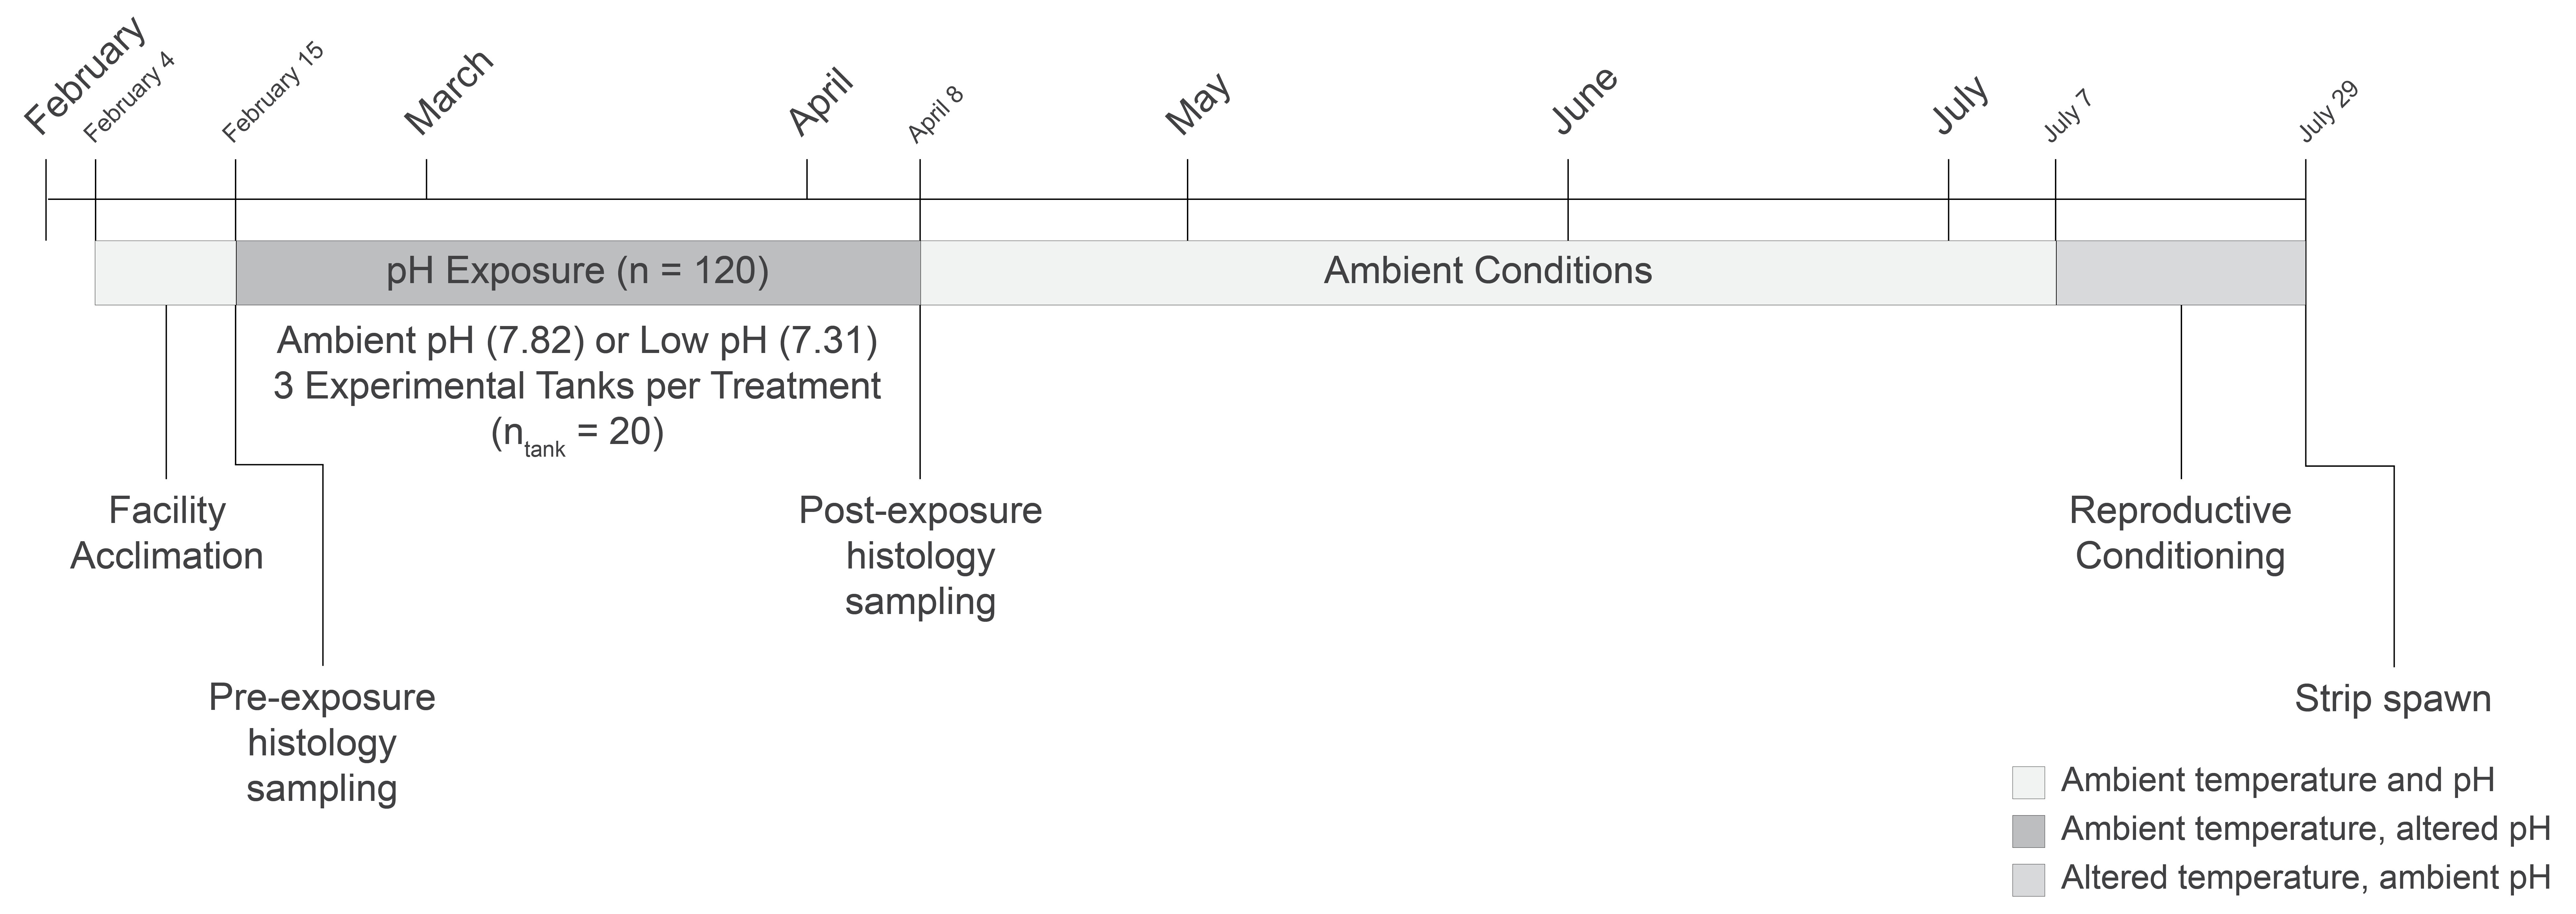
\includegraphics[width=1.3\textwidth]{figure/Ch2/Figure2.1.jpg}
  \caption{Experimental timeline}
  \label{fig:expdesign}
\end{figure}
\end{landscape}
\clearpage

\textbf{Figure} \ref{fig:carryoverboxplot}: Proportion of live D-hinge larvae eighteen hours post-fertilization by female treatment. Each box represents proportions of live larvae between the first and third quartiles for half-sibling families where the female was exposed to either ambient or low pH conditions. Horizontal lines outside the box indicate the minimum value before the lower fence and the maximum value before the upper fence, with the solid line indicating the median. Circles represent outliers. A proportion of 1.0 indicates that all eggs in a cross were successfully fertilized and developed into D-hinge larvae. A linear mixed model, with sire as a random effect, indicated significantly fewer D-hinge larvae were present in half-sibling families where females were exposed to low pH conditions (t = -2.999; p = 0.0119). Significantly different proportions are indicated by a letter.\newline 
\begin{figure}[h]
\centering
  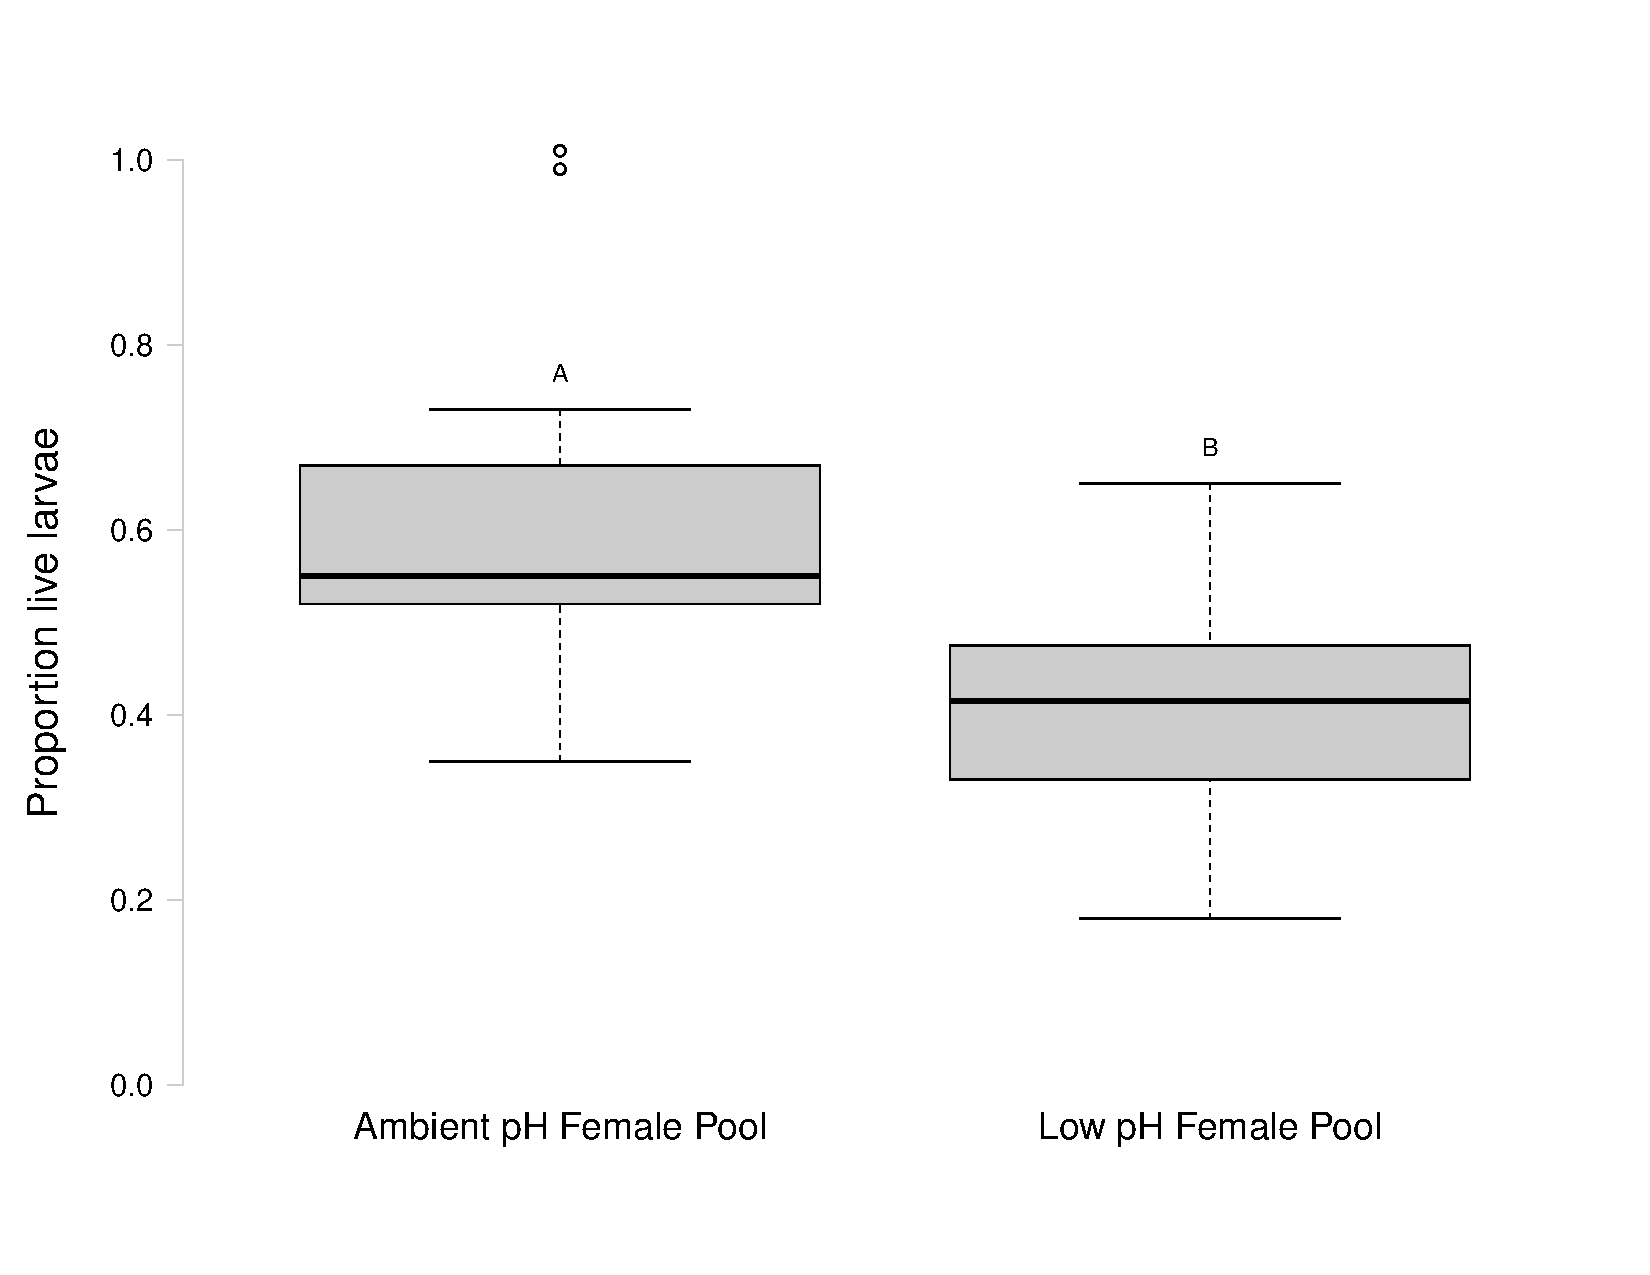
\includegraphics[width=0.85\textwidth]{figure/Ch2/Figure2.2.pdf}
  \caption{Larval survival 18 hours post-fertilization}
  \label{fig:carryoverboxplot}
\end{figure}
\clearpage

\hypertarget{low-ph-influences-methylation-patterns-of-gonad-growth-genes-in-the-pacific-oyster-crassostrea-gigas}{%
\chapter{\texorpdfstring{Low pH influences methylation patterns of gonad growth genes in the Pacific oyster (\emph{Crassostrea gigas})}{Low pH influences methylation patterns of gonad growth genes in the Pacific oyster (Crassostrea gigas)}}\label{low-ph-influences-methylation-patterns-of-gonad-growth-genes-in-the-pacific-oyster-crassostrea-gigas}}

\hypertarget{abstract-2}{%
\section{Abstract}\label{abstract-2}}

There is a need to investigate mechanisms of phenotypic plasticity in marine invertebrates as negative effects of climate change are experienced by coastal ecosystems. Environmentally-induced changes to the methylome can confer plasticity through regulation of gene expression, but methylome responses may be tissue- and species-specific. To assess how ocean acidification affects the Pacific oyster (\emph{Crassostrea gigas}) epigenome, we exposed oysters to either low pH (7.31 ± 0.02) or ambient pH (7.82 ± 0.02) conditions for seven weeks. Whole genome bisulfite sequencing was used to identify methylated regions in female oyster gonad samples. Analysis of gonad methylomes revealed a total of 1,599 differentially methylated loci (DML) were identified and found primarily in genes, with several genes containing multiple DML. Approximately 20\% of DML overlapped with C/T SNPs. Overrepresented biological processes and cellular components in genes containing DML included cilium movement, development, and cytoskeletal components, suggesting that pH-responsive methylation may target gonad growth processes. Since enriched processes were associated with genic DML in multiple transcripts, it is possible DML in these genes could regulate alternative splicing. Our findings provide a foundation for understanding methylation-induced plasticity in \emph{C. gigas}.

\hypertarget{introduction-3}{%
\section{Introduction}\label{introduction-3}}

There is great interest in elucidating how changes in the environment can impact marine invertebrate stress responses, and determining how plastic that phenotype is by examining DNA methylation in marine invertebrates (\protect\hyperlink{ref-Eirin-Lopez2018}{Eirin-Lopez \& Putnam, 2018}; \protect\hyperlink{ref-Hofmann2017}{Hofmann, 2017}). Environmental variation can alter the positions of methyl groups on CpG dinucleotides (\protect\hyperlink{ref-Eirin-Lopez2018}{Eirin-Lopez \& Putnam, 2018}). Methylation does not alter the DNA sequence itself, but can regulate gene expression by fine-tuning expression of housekeeping genes or providing additional transcriptional opportunities for environmental response genes (\protect\hyperlink{ref-Gavery2014}{Gavery \& Roberts, 2014}). Methylation regulation of gene expression could then influence plasticity in response to environmental stressors (\protect\hyperlink{ref-Eirin-Lopez2018}{Eirin-Lopez \& Putnam, 2018}). Ocean acidification (\protect\hyperlink{ref-Bogan2020}{Bogan, Johnson, \& Hofmann, 2020}; \protect\hyperlink{ref-ChandraRajan2021}{Chandra Rajan, Yuan, Yu, Roberts, \& Thiyagarajan, 2021}; \protect\hyperlink{ref-Downey-Wall2020}{Downey-Wall et al., 2020}; \protect\hyperlink{ref-Liew2018b}{Liew, Zoccola, et al., 2018}; \protect\hyperlink{ref-Lim2020}{Lim et al., 2020}; \protect\hyperlink{ref-Venkataraman2020}{Venkataraman et al., 2020}), heat stress (\protect\hyperlink{ref-Arredondo-Espinoza2021}{Arredondo-Espinoza, Ibarra, Roberts, Sicard-Gonzalez, \& Escobedo-Fregoso, 2021}), upwelling conditions (\protect\hyperlink{ref-Strader2019}{M. E. Strader, Wong, Kozal, Leach, \& Hofmann, 2019}), disease (\protect\hyperlink{ref-Johnson2020}{Johnson, Sirovy, Casas, La Peyre, \& Kelly, 2020}), pesticide exposure (\protect\hyperlink{ref-Rondon2017}{Rondon et al., 2017}), and temperature and salinity (\protect\hyperlink{ref-Liew2018a}{Liew, Howells, et al., 2018}) have all elicited changes in marine invertebrate methylomes, demonstrating a potential for methylation to regulate organismal responses to environmental conditions.

Given the impact of ocean acidification on calcifying species like oysters (\protect\hyperlink{ref-Kroeker2010}{Kroeker, Kordas, Crim, \& Singh, 2010}; \protect\hyperlink{ref-Melzner2019}{Melzner, Mark, Seibel, \& Tomanek, 2019}; \protect\hyperlink{ref-Parker2013}{Parker et al., 2013}), several environmental epigenetic studies have examined the influence of ocean acidification on molluscan methylomes (Table 3.1). For example, eastern oyster (\emph{Crassostrea virginica}) mantle (\protect\hyperlink{ref-Downey-Wall2020}{Downey-Wall et al., 2020}) and reproductive tissue (\protect\hyperlink{ref-Venkataraman2020}{Venkataraman et al., 2020}), and Hong kong oyster (\emph{Crassostrea hongkongensis}) mantle (\protect\hyperlink{ref-ChandraRajan2021}{Chandra Rajan, Yuan, Yu, Roberts, \& Thiyagarajan, 2021}), and larval methylomes (\protect\hyperlink{ref-Lim2020}{Lim et al., 2020}) all display changes in DNA methylation after experimental ocean acidification exposure. Between all four studies, only \protect\hyperlink{ref-Venkataraman2020}{Venkataraman et al.} (\protect\hyperlink{ref-Venkataraman2020}{2020}) reports the percent of CpGs methylated: the stated 22\% is consistent with the baseline 15\% methylation observed in initial Pacific oyster (\emph{Crassostrea gigas}) methylation studies (\protect\hyperlink{ref-Gavery2013}{Gavery \& Roberts, 2013}), as well as examination of methylome responses to heat stress (14.4\%; (\protect\hyperlink{ref-Arredondo-Espinoza2021}{Arredondo-Espinoza, Ibarra, Roberts, Sicard-Gonzalez, \& Escobedo-Fregoso, 2021})) and diuron exposure (16.6\%; (\protect\hyperlink{ref-Rondon2017}{Rondon et al., 2017})). In \emph{C. virginica}, the mantle methylome was hypomethylated after ocean acidification exposure (\protect\hyperlink{ref-Downey-Wall2020}{Downey-Wall et al., 2020}), while there were no differences in global gonad methylation patterns (\protect\hyperlink{ref-Venkataraman2020}{Venkataraman et al., 2020}). Experimental ocean acidification exposure yielded differential methylation predominantly in gene bodies, but concentration in exons (\protect\hyperlink{ref-Lim2020}{Lim et al., 2020}; \protect\hyperlink{ref-Venkataraman2020}{Venkataraman et al., 2020}) versus introns (\protect\hyperlink{ref-ChandraRajan2021}{Chandra Rajan, Yuan, Yu, Roberts, \& Thiyagarajan, 2021}) varies. Hyper- and hypomethylation occurs with equal frequency in response to ocean acidification. This is consistent with diuron exposure (\protect\hyperlink{ref-Rondon2017}{Rondon et al., 2017}), but not with heat stress (\protect\hyperlink{ref-Arredondo-Espinoza2021}{Arredondo-Espinoza, Ibarra, Roberts, Sicard-Gonzalez, \& Escobedo-Fregoso, 2021}). Gene functions enriched in differential methylation datasets were inconsistent between species and tissue types (Table 3.1). While aminotransferase complex and biosynthetic processes were found to be enriched in hypomethylated DML in \emph{C. virginica} mantle tissue (\protect\hyperlink{ref-Downey-Wall2020}{Downey-Wall et al., 2020}), there were no enriched GOterms associated with genic DML in \emph{C. virginica} gonad samples (\protect\hyperlink{ref-Venkataraman2020}{Venkataraman et al., 2020}). In contrast, several processes were enriched in methylation datasets for \emph{C. hongkongensis}, including acetoacetylco-A reductase activity, dehydrogenase activity, cellular response to pH, protein xylosyltransferase activity, translation factor activity, RNA binding, and diacylglycerol kinase activity in the mantle (\protect\hyperlink{ref-ChandraRajan2021}{Chandra Rajan, Yuan, Yu, Roberts, \& Thiyagarajan, 2021}) and cytoskeletal and signal transduction, oxidative stress, metabolic processes, and larval metamorphosis in larvae (\protect\hyperlink{ref-Lim2020}{Lim et al., 2020}). While considerable effort has been made to understand molluscan methylation responses to ocean acidification, it is clear that there may be species- and tissue-specific responses. Additionally, use of enrichment methods prior to bisulfite conversion and sequencing in previous studies may impact functional interpretation differential methylation data (\protect\hyperlink{ref-Trigg2021}{Trigg et al., 2021}).

In addition to being an important global aquaculture species, \emph{C. gigas} has been used to further our understanding of methylation in marine invertebrates (\protect\hyperlink{ref-Gavery2013}{Gavery \& Roberts, 2013}, \protect\hyperlink{ref-Gavery2014}{2014}, \protect\hyperlink{ref-Gavery2017}{2017}; \protect\hyperlink{ref-Olson2014}{Olson \& Roberts, 2014}, \protect\hyperlink{ref-Olson2015}{2015}; \protect\hyperlink{ref-Riviere2013}{Riviere et al., 2013}, \protect\hyperlink{ref-Riviere2017}{2017}; \protect\hyperlink{ref-Roberts2012}{Roberts \& Gavery, 2012}; \protect\hyperlink{ref-Saint-Carlier2015}{Saint-Carlier \& Riviere, 2015}; \protect\hyperlink{ref-Song2017}{Song, Li, \& Zhang, 2017}). Examination of diuron exposure (\protect\hyperlink{ref-Rondon2017}{Rondon et al., 2017}) and heat stress on different \emph{C. gigas} phenotypes (\protect\hyperlink{ref-Arredondo-Espinoza2021}{Arredondo-Espinoza, Ibarra, Roberts, Sicard-Gonzalez, \& Escobedo-Fregoso, 2021}) reveal that environmental conditions do influence the Pacific oyster methylome, and other oyster methylomes are responsive to ocean acidification (Table 3.1). However, studies examining the influence of ocean acidification on the \emph{C. gigas} methylome are currently absent. Additionally, a recent study found that female \emph{C. gigas} exposure to low pH conditions, followed by four months in ambient pH conditions prior to spawning, can still negatively impact larval survival 18 hours post-fertilization (\protect\hyperlink{ref-Venkataraman2019}{Venkataraman, Spencer, \& Roberts, 2019}). Since maturation stage was not different between female \emph{C. gigas} after low pH exposure, this finding suggests environmental ``memory'' may be mediating the carryover effect.

We sought to understand impacts of ocean acidification on the Pacific oyster gonad methylome in order to not only understand DNA methylation as a potential mechanism for the observed negative maternal carryover effect previously reported in \protect\hyperlink{ref-Venkataraman2019}{Venkataraman, Spencer, \& Roberts} (\protect\hyperlink{ref-Venkataraman2019}{2019}), but to also examine the functional role of methylation in regulating biological responses to ocean acidification. Female oyster gonad methylome sequencing revealed distinct methylation changes associated with low pH exposure. These results provide the foundation for examining phenotypic plasticity within a generation, as well as larval methylomes and potential intergenerational effects.

\hypertarget{methods-2}{%
\section{Methods}\label{methods-2}}

\hypertarget{experimental-design}{%
\subsection{Experimental Design}\label{experimental-design}}

The experimental design and seawater chemistry analysis with carbon chemistry parameters are described in \protect\hyperlink{ref-Venkataraman2019}{Venkataraman, Spencer, \& Roberts} (\protect\hyperlink{ref-Venkataraman2019}{2019}). Briefly, adult hatchery-raised \emph{C. gigas} (average shell length = 117.46 ± 19.16 cm) were exposed to either low pH (7.31 ± 0.02) or ambient pH (7.82 ± 0.02) conditions from February 15, 2017 to April 8, 2017 at the Kenneth K. Chew Center for Shellfish Research and Restoration at the National Oceanic and Atmospheric Administration Manchester Field Station (47º 34' 09.1'' N 122º 33' 19.0'' W, Manchester, WA). Shell length, width, and oyster wet weight were obtained before and after pH exposure, and gonad tissue was extracted for histological analysis at each sampling point. Prior to exposure, twenty \emph{C. gigas} were randomly selected for histology, while ten oysters from each treatment were randomly selected from tanks to assess maturation. Gonad tissue in cassettes was fixed for histology using PAXgene Tissue Fix and Stabilizer and sent to Diagnostic Pathology Medical Group, Inc.~(Sacramento, CA) for hematoxylin and eosin staining and slide preparation. Tissues exposed to ambient pH were confounded during processing, preventing any tank identification. Maturation state and organism sex was evaluated histologically at 40x magnification (\protect\hyperlink{ref-Enriquez-Diaz2008}{Enrı́quez-Dı́az, Pouvreau, Chávez-Villalba, \& Le Pennec, 2008}; \protect\hyperlink{ref-Fabioux2005}{Fabioux, Huvet, Le Souchu, Le Pennec, \& Pouvreau, 2005}).

\hypertarget{dna-extraction-and-library-preparation}{%
\subsection{DNA Extraction and Library Preparation}\label{dna-extraction-and-library-preparation}}

To determine how pH exposure altered maternal gonad methylation, DNA was extracted from histology blocks for four female (or presumed female) oysters for each treatment using the PAXgene Tissue DNA Kit (Qiagen) with modifications specified below at the end of the seven-week exposure. For each sample, up to 0.02 g of histology tissue embedded in paraffin was cut from the histology block and placed in a 2 mL round-bottomed tube. The tissue was then further homogenized within the tube. After adding 1 mL of xylene, each sample was vortexed for 20 seconds, incubated at room temperature for three minutes, then centrifuged at maximum speed for three minutes. To evaporate ethanol from samples after ethanol addition and vortexing steps, samples were placed on a heat block at 37ºC for 10-20 minutes to evaporate any residual ethanol.

The resuspended pellet was lysed using a TissueTearor at setting 1. Prior to lysis and between samples, the TissueTearor was run in a 10\% bleach solution for 20 seconds, followed by two consecutive 20 second runs in DI water to clean the instrument. Lysates were transferred to clean, labelled 1.5 mL microcentrifuge-safelock tubes. Proteinase K (20 µL) was added to each sample, and pulse-vortexed for 15 seconds to mix. The sample-Proteinase K solution was incubated 56ºC for 60 minutes. Every ten minutes, the samples were briefly removed from the heat block to vortex at maximum speed for one minute. After 60 minutes, RNase A (4 µL, 100 mg/mL) was added to each sample. Samples were vortexed at maximum speed for 20 seconds to mix and incubated for two minutes at room temperature to obtain RNA-free genomic DNA and reduce possible interference for downstream enzyme reactions. Samples were then kept at 80ºC for 60 minutes, and vortexed at maximum speed for one minute in ten-minute intervals. After the incubation, Buffer TD2 and 200 µL ethanol were added to each sample, vortexing thoroughly to mix.

DNA was isolated for each sample after lysis and incubation following manufacturer's instructions. To elute DNA, samples were loaded onto the spin column with Buffer TD5 (50 µL) and incubated at room temperature for five minutes to increase yield, then centrifuged at maximum speed for one minute. A Qubit™ 3.0 and dsDNA BR Assay (Invitrogen) was used to quantify sample yield using 1 µL of DNA for each sample. For two samples, DNA was further concentrated using an ethanol precipitation.

Samples were sent to ZymoResearch for bisulfite conversion and library preparation. Bisulfite conversion was performed with the Zymo-Seq WGBS Library Kit (Cat. \#D5465) using 100 ng of genomic DNA following manufacturer's instructions. Per ZymoResearch protocol, samples were spiked with a mixture of six unique double-stranded synthetic amplicons (180-200 bp) from the \emph{Escherichia coli} K12 genome. Since each amplicon represents a different percent methylation, the spike-in was used to determine bisulfite conversion efficiency. Libraries were barcoded and pooled into a single lane to generate 150 bp paired-end reads in a single Illumina NovaSeq flowcell.

\hypertarget{genome-information-and-feature-tracks}{%
\subsection{Genome Information and Feature Tracks}\label{genome-information-and-feature-tracks}}

Nuclear (\protect\hyperlink{ref-Penaloza2021}{Peñaloza et al., 2021}) (NCBI GenBank: GCA\_902806645.1, RefSeq: GCF\_902806645.1) and mitochondrial genome sequences (NCBI Reference Sequence: NC\_001276.1) were used in downstream analysis. These sequences were combined for downstream alignment. The \texttt{fuzznuc} function within EMBOSS was used to identify CG motifs in the combined genomes.

The RefSeq annotation was used to obtain genome feature tracks, and create additional tracks. The annotation included a combination of Gnomon, RefSeq, cmsearch, and tRNAscan-SE predictions. Gene, coding sequence, exon, and lncRNA tracks were extracted from the RefSeq annotation. These tracks were then used to obtain additional genome feature information. To create an intron track, the complement of the exon track was generated with BEDtools \texttt{complementBed} v.2.26.0 to create a non-coding sequence track (\protect\hyperlink{ref-Quinlan2010}{Quinlan \& Hall, 2010}). The overlap between the genes and the non-coding sequences was found with \texttt{intersectBed} and defined as introns. Similarly, untranslated regions of exons were obtained by subtracting coding sequences from exon information with \texttt{subtractBed}. Flanking regions were defined as the 1000 bp upstream or downstream of genes. Upstream flanks were generated by adding 1000 bp upstream of genes, taking into account strand, with \texttt{flankBed}. Existing genes were removed from flanking sequences using \texttt{subtractBed}. A similar process was performed to generate downstream flanking regions. Intergenic regions were isolated by finding the complement of genes with \texttt{complementBed}, then using subtractBed to remove any flanks. Transposable element locations were obtained from RepeatMasker using the NCBI RefSeq annotation (RefSeq: GCF\_902806645.1) (Smit et al., 2013; Tarailo-Graovac \& Chen, 2009). The number of CG motifs in a given feature track was obtained using \texttt{intersectBed}.

\hypertarget{sequence-alignment}{%
\subsection{Sequence Alignment}\label{sequence-alignment}}

Reads were trimmed three times prior to alignment using TrimGalore! v.0.6.6 (\protect\hyperlink{ref-Martin2011}{Martin, 2011}). Known Illumina adapter sequences were removed (\texttt{-\/-illumina}), along with 10 bp from both the 5' (\texttt{-\/-clip\_R1\ 10} and \texttt{-\/-clip\_R2\ 10}) and 3' ends of 150 bp paired-end reads (\texttt{-\/-three\_prime\_clip\_R1\ 10} and \texttt{-\/-three\_prime\_clip\_R2\ 10}). Any remaining adapters were removed in a second round of trimming. Finally, poly-G tails were trimmed out of samples by manually specifying adapter sequences (\texttt{-\/-adapter\ GGGGGGGGGGGGGGGGGGGGGGGGGGGGGGGGGGGGGGGGGGGGGGGGGG} and \texttt{-\/-adapter2\ GGGGGGGGGGGGGGGGGGGGGGGGGGGGGGGGGGGGGGGGGGGGGGGGGG}). Sequence quality was assessed with FastQC v.0.11.9 (\protect\hyperlink{ref-Andrews2010}{Andrews, 2010}) and MultiQC (\protect\hyperlink{ref-Ewels2016}{Ewels, Magnusson, Lundin, \& Käller, 2016}) after each round of trimming.

Trimmed samples were then aligned to the combined nuclear and mitochondrial genomes for \emph{C. gigas} (\protect\hyperlink{ref-Penaloza2021}{Peñaloza et al., 2021}). The genome was bisulfite converted with Bowtie 2-2.3.4 (Linux x84\_64 version (\protect\hyperlink{ref-Langmead2012}{Langmead \& Salzberg, 2012})) using the bismark\_genome\_preparation function within Bismark v.0.22.3 (\protect\hyperlink{ref-Krueger2011}{Krueger \& Andrews, 2011}). Reads were aligned to the bisulfite-converted genome. Non-directional input was specified (\texttt{-\/-non\_directional}), and alignment scores could be no lower than -90 (\texttt{-score\_min\ L,0,-0.6}). Resultant BAM files were deduplicated (\texttt{-\/-deduplicate\_bismark}), and methylation calls were extracted from deduplicated BAM files (\texttt{bismark\_methylation\_extractor}). Deduplicated BAM files were also sorted and indexed for downstream applications using SAMtools v.1.10 (\protect\hyperlink{ref-Li2009}{Li et al., 2009}). Using coverage files generated from methylation extraction, CpG information was consolidated between strands to report 1-based chromosomal coordinates (\texttt{coverage2cystosine}). Using coverage2cytosine coverage file output, genomic coordinates for CpGs with at least 5x coverage across all samples were written to BEDgraphs. Summary reports with alignment information for each sample were generated (\texttt{bismark2report} and \texttt{bismark2summary}) and concatenated with MultiQC. Code for all sequence alignment steps can be found in the associated Github repository (\url{https://github.com/RobertsLab/project-gigas-oa-meth}).

\hypertarget{snp-identification}{%
\subsection{SNP Identification}\label{snp-identification}}

As genomic differences can play a role in methylation, single nucleotide polymorphisms (SNPs) were identified from WGBS data to determine if they overlapped with differentially methylated loci. SNP variants across all samples and in individuals were identified with \texttt{BS-Snper} (\protect\hyperlink{ref-Gao2015}{Gao et al., 2015}). As \texttt{BS-Snper} only takes one input file, deduplicated and sorted BAM alignments generated with Bismark v.0.22.3 and SAMtools v.1.10 (\protect\hyperlink{ref-Krueger2011}{Krueger \& Andrews, 2011}; \protect\hyperlink{ref-Li2009}{Li et al., 2009}) were merged (\texttt{samtools\ merge}). Variants were then identified in the merged BAM file or individual deduplicated and sorted BAM files. Default \texttt{BS-Snper} settings were used, except for a minimum coverage of 5x to be consistent with methylation analyses. C/T SNPs were filtered by identifying overlaps between SNPs and CG motifs with intersectBed. The C/T SNPs were used in downstream analyses to identify differentially methylated loci that overlapped with SNPs.

\hypertarget{global-methylation-characterization}{%
\subsection{Global Methylation Characterization}\label{global-methylation-characterization}}

Global methylation patterns were characterized averaging DNA methylation across all samples (using a 5x coverage threshold). A CpG locus was considered highly methylated if average percent methylation was greater than or equal to 50\%, moderately methylated if percent methylation was between 10-50\%, and lowly methylated if percent methylation was less than or equal to 10\%. The genomic location of highly, moderately, and lowly methylated CpGs in relation to UTR, CDS, introns, up- and downstream flanking regions, transposable elements, and intergenic regions were determined by using intersectBed. We tested the null hypothesis that there was no association between the genomic location of CpG loci and methylation status (all CpGs versus highly methylated CpGs) with a chi-squared contingency test (\texttt{chisq.test} in R Version 3.5.3 (\protect\hyperlink{ref-R_Core_Team2019}{R Core Team, 2019})).

\hypertarget{identification-of-differentially-methylated-loci}{%
\subsection{Identification of Differentially Methylated Loci}\label{identification-of-differentially-methylated-loci}}

Identification of differentially methylated loci, or DML, was conducted with \texttt{methylKit} v.1.17.4 (\protect\hyperlink{ref-Akalin2012}{Akalin et al., 2012}) in R Version 3.5.3 (\protect\hyperlink{ref-R_Core_Team2019}{R Core Team, 2019}). Prior to DML identification, data were imported and processed. Data with at least 2x coverage were imported using \texttt{methRead} from merged CpG coverage files produced by \texttt{coverage2cytosine}. Imported data were filtered again (\texttt{filterByCoverage}) to require 5x coverage for each CpG locus (\texttt{lo.count\ =\ 5}) in each sample. Potential PCR duplicates in each sample were also removed by excluding CpG loci in the 99.9th percentile of coverage (\texttt{high.perc\ =\ 99.9}). Once filtered, data were normalized across samples (\texttt{normalizeCoverage}) to avoid over-sampling reads from one sample during downstream statistical analysis. Histograms of percent methylation (\texttt{getMethylationStats}) and CpG coverage (\texttt{getCoverageStats}) were used to confirm normalization. After filtering and normalization, data at each CpG locus with 5x were combined (\texttt{unite}) to create a CpG background, ensuring that each locus had at least 5x coverage in each sample.

Methylation differences were then identified for \emph{C. gigas} gonad samples. A logistic regression (\texttt{calculateDiffMeth}) modeled the log odds ratio based on the proportion of methylation at each CpG locus. A covariate matrix with gonad stage information (\texttt{covariates}) were applied to the model for the \emph{C. gigas} data to account for varying maturation stages in samples. Additionally, an overdispersion correction with a chi-squared test (\texttt{overdispersion\ =\ "MN",\ test\ =\ "Chisq"}) was applied.

Differentially methylated loci, or DML, were defined as CpG dinucleotides with at least a 50\% methylation difference between pH treatments, and a q-value \textless{} 0.01 based on correction for false discovery rate with the SLIM method (\protect\hyperlink{ref-Wang2011}{H.-Q. Wang, Tuominen, \& Tsai, 2011}). Hypermethylated DML were defined as those with significantly higher percent methylation in low pH samples, and hypomethylated DML with significantly lower percent methylation in low pH samples. BEDfiles with DML locations were created and viewed with the Integrative Genomics Viewer (IGV) version 2.9.2 (\protect\hyperlink{ref-Thorvaldsdottir2013}{Thorvaldsdóttir, Robinson, \& Mesirov, 2013}).

\hypertarget{dml-characterization}{%
\subsection{DML Characterization}\label{dml-characterization}}

The location of DML was characterized in relation to various genome feature tracks. Presence of DML in UTR, CDS, introns, up- and downstream flanking regions, transposable elements, and intergenic regions was discerned using intersectBed. A chi-squared contingency test was used to test the null hypothesis of no association between genomic location and differential methylation by comparing the genomic location of all CpGs with 5x data and DML. Additionally, the number of DML present in each chromosome was quantified to see if DML were distributed uniformly across the genome. Overlaps between DML and SNPs were identified to determine if DML were solely attributed to treatment differences, or if genetic differences contributed to differential methylation.

\hypertarget{enrichment-analysis}{%
\subsection{Enrichment Analysis}\label{enrichment-analysis}}

To determine if genes containing DML were associated with overrepresented biological processes, cellular component, or molecular function gene ontologies (GO), we conducted functional enrichment analysis. Prior to this analysis, the \emph{C. gigas} genome was annotated. A \texttt{blastx} was performed against the Uniprot-SwissProt database (accessed June 01, 2021) to get Uniprot Accession information for each transcript (\protect\hyperlink{ref-UniProt_Consortium2019}{UniProt Consortium, 2019}). The transcript nucleotide sequences were extracted from the genome (GCF\_902806645.1\_cgigas\_uk\_roslin\_v1\_rna\_from\_genomic.fna available in the NCBI Annotation Release 102). Transcript IDs from the \texttt{blastx} output were matched with GO terms from the Uniprot-Swissprot database using Uniprot Accession codes. These transcript IDs and corresponding GO terms were then used to create a gene ID-to-GO term database (\texttt{geneID2GO}) for manual GO term annotation. The transcript IDs were filtered for genes that contained CpGs with at least 5x coverage in all samples, as the same parameters were used to generate the CpG background for differential methylation analysis. Each line of the database contained transcript ID in one column, and all corresponding GO terms in another column.

Gene enrichment analysis was conducted with \texttt{topGO} v.2.34.0 in R (\protect\hyperlink{ref-Alexa2010}{Alexa, Rahnenfuhrer, \& Others, 2010}). The \texttt{geneID2GO} database was used as the gene universe for enrichment, while transcript IDs for genes with DML were used as the genes of interest. These transcript IDs were filtered such that they did not include any transcripts associated with DML-SNP overlaps. A \texttt{topGO} object was generated for each DML list and GO category (biological process, cellular component, or molecular function), with GO term annotation performed using the \texttt{geneID2GO} database. A Fisher's exact test was used to identify GO terms in each DML list significantly enriched with respect to the gene background (P-value \textless{} 0.01). Keeping with \texttt{topGO} default settings, we did not correct for multiple comparisons (\protect\hyperlink{ref-Alexa2010}{Alexa, Rahnenfuhrer, \& Others, 2010}). Visualization of enriched GO terms was conducted using \texttt{simplifyEnrichment} v.1.2.0 default settings (\protect\hyperlink{ref-Gu2021}{Gu \& Hübschmann, 2021}). Briefly, a semantic similarity matrix was created from enriched GO IDs using the ``Relevance'' similarity measure and GO tree topology (\texttt{GO\_similarity}). The semantic similarity matrix was clustered using the binary cut method, and visualized as a word cloud alongside a heatmap of semantic similarity (\texttt{simplifyGO}).

\hypertarget{results-2}{%
\section{Results}\label{results-2}}

\hypertarget{sequence-alignment-1}{%
\subsection{Sequence Alignment}\label{sequence-alignment-1}}

Whole genome bisulfite sequencing produced 1.38 x 10\textsuperscript{9} total 150 bp paired-end reads. After quality trimming, 1.35 x 10\textsuperscript{9} total paired reads remained (Appendix 1). Of the trimmed paired-end reads, 8.31 x 108 (61.7\%) were uniquely aligned to the bisulfite-converted \emph{C. gigas} genome with appended mitochondrial sequence (Appendix 1).

\hypertarget{snp-identification-1}{%
\subsection{SNP Identification}\label{snp-identification-1}}

C/T SNP variants were identified from WGBS data to determine if genomic differences contributed to differential methylation. A total of 13,234,183 unique SNPs were found in individual or merged BAM files, including 300,278 C/T SNPs. These C/T SNPs were used in downstream analyses (see \emph{DML Characterization and Enrichment Analysis}).

\hypertarget{global-methylation-patterns}{%
\subsection{Global Methylation Patterns}\label{global-methylation-patterns}}

When data were combined, using a 5x coverage threshold 11,238,223 CpG loci (84.8\% of 13,246,547 total CpGs in \emph{C. gigas} genome) were characterized. The majority of CpGs, 9,201,922 loci (81.9\%) were lowly methylated, followed by 1,029,894 highly methylated (9.2\%) and 1,006,406 moderately methylated (9.0\%) CpGs. Highly methylated CpGs were found primarily in genic regions (964,976 CpGs, 93.7\%), with 57,896 (5.6\%) in exon UTR, 355,575 (34.5\%) in CDS, and 554,093 (53.8\%) in introns (Figure \ref{fig:fembackground}). The distribution of highly methylated CpGs was significantly different than all 5x CpGs detected by WGBS (Appendix 1). A Principal Component Analysis (PCA) did not demonstrate any clear separation of samples by treatment, and consistently high Pairwise Pearson's correlation coefficients support the lack of global percent methylation differences between pH treatments (Appendix 1).

\hypertarget{dml-characterization-1}{%
\subsection{DML Characterization}\label{dml-characterization-1}}

A total of 1,599 DML were identified using a 50\% methylation difference threshold (Figure \ref{fig:femheatmap}), which were evenly split between 793 (49.6\%) hypomethylated and 806 (50.4\%) hypermethylated DML (Figure \ref{fig:femheatmap}). Of these DML, 315 (19.7\%) overlapped with C/T SNPs. The DML were distributed amongst the ten main chromosomes, as well as scaffolds not placed in any chromosome (Figure @ref(fig: chromdistr), Appendix 1).

The majority of DML (1,478; 92.4\%) were located in genic regions (Figure @ref(fig: locDML)), consisting of 1080 unique genes. Most genes only contained one DML; however, several genes contained multiple DML, ranging from 2-104 DML in one gene (Appendix 1). The genic DML were primarily located in introns (941; 58.8\%), followed by CDS (442; 27.6\%) and exon UTR (95; 5.9\%). Putative promoter regions upstream of transcription start sites contained DML (12; 0.8\%), but more were located in downstream flanking regions (73; 4.6\%). Additionally, 297 of the 1,478 genic DML overlapped with C/T SNPs in 283 unique genes. The DML were also found in transposable elements (496; 31.0\%), lncRNA (9; 0.6\%), and intergenic regions (42; 2.6\%). The number of DML in all genome features differed significantly from all 5x CpGs (Appendix 1).

\hypertarget{enrichment-analysis-1}{%
\subsection{Enrichment Analysis}\label{enrichment-analysis-1}}

We identified 10 biological processes and 4 molecular function GOterms significantly enriched in genes containing DML that did not overlap with C/T SNPs (Figure @ref(fig: simplifyEnrichment), Appendix 1). A total of 339 genes with GOterm annotations containing 437 DML were used for this analysis. The enriched biological process GOterms were involved in motility (ex. cilium-dependent cell motility, cilium movement) and development (insta larval or pupal development, post-embryonic development), while the cellular component GOterms were involved in microtubule-associated and histone acetyltransferase complexes (Appendix 1). A total of 7 unique genes and 34 unique transcripts were associated with the biological process terms, and 2 unique genes and 15 unique transcripts were associated with cellular component terms (Appendix 1).

\hypertarget{discussion-2}{%
\section{Discussion}\label{discussion-2}}

Our work examined the potential role of environmentally-induced changes to the reproductive tissue methylome to mediate carryover effects in \emph{C. gigas}. We identified a total of 1,599 differentially methylated loci, showing that the methylome is responsive to ocean acidification. We also found significantly enriched biological processes associated with genic DML, implying that low pH may impact regulation of distinct processes, such as gonad development. We also highlight the importance of understanding genomic contributions to differential methylation through the identification of SNPs that overlap with DML. Our findings contribute to the growing body of work examining epigenetic responses in molluscan species, and provide the foundation for future research examining intergenerational epigenetic inheritance and its potential to mediate plastic responses to environmental stressors.

The enriched GOterms associated with genes containing DML suggest environmentally-responsive methylation can regulate gonad growth processes. Enrichment of cilium movement and overrepresentation of microtubule-associated complexes could be related to changes in cytoskeletal structure. These changes may signify reorganization of female reproductive tissue to accommodate growing oocytes, or a need to regulate protein transport and cytoskeletal activity. Differentially methylated genes in \emph{C. hongkongensis} larvae exposed to ocean acidification also were enriched in cytoskeletal processes (\protect\hyperlink{ref-Lim2020}{Lim et al., 2020}), suggesting that this particular process may be targeted by methylation across life stages. In female oysters, expression of microtubule-associated genes increases from stage 0 to 2, but decreases after stage 3 (\protect\hyperlink{ref-Dheilly2012}{Dheilly et al., 2012}). As \protect\hyperlink{ref-Venkataraman2019}{Venkataraman, Spencer, \& Roberts} (\protect\hyperlink{ref-Venkataraman2019}{2019}) did not identify any difference in maturation stage between oysters in low and ambient pH conditions, methylation regulation of these cytoskeletal genes may have allowed oysters in low pH to maintain gonad growth at the same rate as those in ambient pH conditions. It is also possible that the mixed cell types used in samples could be influencing enrichment results. Microtubule-associated genes are also present in somatic tissue (\protect\hyperlink{ref-Dheilly2012}{Dheilly et al., 2012}), so changes to the somatic tissue methylation may have also been captured in our analyses as we did not separate cell types. A similar study of \emph{C. virginica} reproductive tissue did not find enrichment of growth processes, which may be due to confounding factors such as mixed cell types, as well as mixed sex and maturation stage in samples (\protect\hyperlink{ref-Venkataraman2020}{Venkataraman et al., 2020}). By using females of known maturation stage, we were able to identify processes influenced by low pH in gonad tissue. Future work should separate different cell types to understand environmentally-responsive methylation specifically in gonad cells.

Additional functions associated with genes containing DML provide insight into potential mechanisms mediating the negative maternal carryover effect observed in \protect\hyperlink{ref-Venkataraman2019}{Venkataraman, Spencer, \& Roberts} (\protect\hyperlink{ref-Venkataraman2019}{2019}){]}. Enriched biological processes associated with development were involved in larval or post-embryonic development, suggesting methylation regulation of genes that may be important for early life-stages. The most common functions associated with genes containing DML were related to hormone signaling, secretion, and metabolism. Whether acidification alters invertebrate reproductive hormones is not yet known, but alterations to hormone pathways through DNA methylation may impact maturation. While there was no difference in female maturation status after the seven-week pH exposure (\protect\hyperlink{ref-Venkataraman2019}{Venkataraman, Spencer, \& Roberts, 2019}), persistent changes to expression of genes related to hormonal processes could impact oyster gametogenesis. Several genes involved in lipid metabolism and biomineralization also contained DML. Reduction in lipid content has been observed in the Sydney rock oyster \emph{S. glomerata} exposed to experimental acidification conditions, but this lipid content reduction did not yield negative effects on embryonic development (\protect\hyperlink{ref-Scanes2018}{Scanes, Parker, O'Connor, Gibbs, \& Ross, 2018}), so the connection between adult \emph{C. gigas} low pH exposure, maternal provisioning, and poor larval survival may not be supported. Several studies note impacts of adult pH exposure on larval calcification process. For example, \emph{S. glomerata} larvae exhibit faster shell growth in high pCO\textsubscript{2} conditions when parents mature in those same conditions (\protect\hyperlink{ref-Parker2012}{Parker et al., 2012}; \protect\hyperlink{ref-Parker2015}{Parker, O'Connor, Raftos, Pörtner, \& Ross, 2015}). In contrast, larvae from other species found in the North Atlantic such as northern quahog (= hard clam; \emph{Mercenaria mercenaria}) and bay scallops (\emph{Argopecten irradians}) developed slower when parents were reproductively conditioned in low pH conditions (\protect\hyperlink{ref-Griffith2017}{Griffith \& Gobler, 2017}). It is possible that \emph{C. gigas} larvae experienced reductions in calcification which lead to lower survival after adult low pH exposure. Additional research is required to discern if methylation changes to hormone signaling, lipid metabolism, and biomineralization genes persist in larvae, and how those changes may influence larval gene expression or survival.

In \emph{C. gigas}, low pH may elicit methylation changes in genes to improve transcriptional control and maintain homeostasis. Differential methylation was found primarily in introns and exons, which suggests that these loci may influence gene expression. This finding is consistent with the literature examining molluscan methylome responses to ocean acidification (\protect\hyperlink{ref-ChandraRajan2021}{Chandra Rajan, Yuan, Yu, Roberts, \& Thiyagarajan, 2021}; \protect\hyperlink{ref-Downey-Wall2020}{Downey-Wall et al., 2020}; \protect\hyperlink{ref-Lim2020}{Lim et al., 2020}; \protect\hyperlink{ref-Venkataraman2020}{Venkataraman et al., 2020}), disease (\protect\hyperlink{ref-Johnson2020}{Johnson, Sirovy, Casas, La Peyre, \& Kelly, 2020}), pesticide exposure (\protect\hyperlink{ref-Rondon2017}{Rondon et al., 2017}), and heat stress (\protect\hyperlink{ref-Arredondo-Espinoza2021}{Arredondo-Espinoza, Ibarra, Roberts, Sicard-Gonzalez, \& Escobedo-Fregoso, 2021}), as well as environmental responses in corals (\protect\hyperlink{ref-Liew2018b}{Liew, Zoccola, et al., 2018}; \protect\hyperlink{ref-Liew2018a}{Liew, Howells, et al., 2018}), urchins (\protect\hyperlink{ref-Strader2019}{M. E. Strader, Wong, Kozal, Leach, \& Hofmann, 2019}), and pteropods (\protect\hyperlink{ref-Bogan2020}{Bogan, Johnson, \& Hofmann, 2020}). The relationship between methylation and gene expression has been investigated in \emph{C. gigas}. High levels of methylation in genes were associated with increased gene expression and low expression variability, implying that methylation leads to transcriptional stability (\protect\hyperlink{ref-Gavery2013}{Gavery \& Roberts, 2013}; \protect\hyperlink{ref-Olson2014}{Olson \& Roberts, 2014}). Methylation was also found to reduce transcriptional noise in response to ocean acidification in corals (\protect\hyperlink{ref-Liew2018b}{Liew, Zoccola, et al., 2018}). While pH-influenced differential methylation was not found to impact gene expression directly in \emph{C. virginica} (\protect\hyperlink{ref-Downey-Wall2020}{Downey-Wall et al., 2020}) or \emph{C. hongkongensis} (\protect\hyperlink{ref-ChandraRajan2021}{Chandra Rajan, Yuan, Yu, Roberts, \& Thiyagarajan, 2021}), neither study investigated methylation connections with alternative splicing. As enriched biological process GOterms were found in various transcripts within genes, there may be a role for methylation regulation of expression regulation via alternative splicing. Additionally enrichment of GOterms related to histone acetyltransferases could be indicative of chromatin regulation, which would then impact methylation and gene expression (ex. \protect\hyperlink{ref-Gatzmann2018}{Gatzmann et al.} (\protect\hyperlink{ref-Gatzmann2018}{2018})). Both elevated temperature and low pH conditions have been found to influence methylation of histone-related genes in \emph{C. gigas} (\protect\hyperlink{ref-Arredondo-Espinoza2021}{Arredondo-Espinoza, Ibarra, Roberts, Sicard-Gonzalez, \& Escobedo-Fregoso, 2021}) and \emph{C. hongkongensis} (\protect\hyperlink{ref-ChandraRajan2021}{Chandra Rajan, Yuan, Yu, Roberts, \& Thiyagarajan, 2021}; \protect\hyperlink{ref-Lim2020}{Lim et al., 2020}). Our findings suggest that the connection between methylation and gene expression requires additional investigation when considering environmental response, with specific inclusion of mechanisms like alternative splicing and chromatin regulation.

Confounding elements may have influenced gonad methylome responses to ocean acidification, and our interpretation of those responses. Although specimens used were sibling oysters in an effort to reduce genomic variation, we identified several SNPs that overlapped with DML. It is possible that the DML algorithm used is biased towards identification of DML that overlap with SNP variants, as it removes individual variation (\protect\hyperlink{ref-Feng2014}{Feng, Conneely, \& Wu, 2014}). With a limited sample size, SNP identification from WGBS is useful for evaluating if DML are solely environmentally-induced, or if genomic variation influences methylation differences. Inclusion of DML that overlap SNPs during enrichment analysis may also confound results, leading to a different biological interpretation. Additionally, the lack of annotated genes used in the enrichment analysis limits our interpretation of which processes are most impacted by pH-sensitive methylation.

Maturation stage is known to produce distinct baseline methylation patterns in \emph{C. gigas} (\protect\hyperlink{ref-Zhang2018}{X. Zhang, Li, Kong, \& Yu, 2018}). While the overall maturation stage was used as a covariate when identifying DML, it is possible that each sample methylome contains information from cells with various maturation stages or cell types. Even though methylation differences in genic regions support our conclusion that low pH does impact the \emph{C. gigas} gonad methylome, single-cell sequencing efforts or investigations within a single maturation stage would clarify how these sources of variation influenced our findings.

\hypertarget{conclusion-2}{%
\section{Conclusion}\label{conclusion-2}}

Our work --- which is the first to explore methylation responses to ocean acidification in Pacific oysters --- found that low pH treatment altered the \emph{C. gigas} female gonad methylome after a seven-week exposure. We found that differential methylation occurs primarily in genic regions, which is consistent with other studies examining oyster methylome responses to ocean acidification. In conjunction with histology data from \protect\hyperlink{ref-Venkataraman2019}{Venkataraman, Spencer, \& Roberts} (\protect\hyperlink{ref-Venkataraman2019}{2019}), enriched biological processes and cellular components in genes containing DML suggest that methylation may be used to maintain gonad growth in low pH conditions. Our work expands on previous molluscan methylation research by not only demonstrating a potential role for methylation in plastic responses to ocean acidification, but also incorporating removing genomic variation from analysis to strengthen biological interpretation of data.

As inheritance of environmentally-induced methylation --- and any resulting phenotypic plasticity --- is contingent on epigenetic marks being present in the germline, withstanding chromatin reorganization, and being packaged into gametes (\protect\hyperlink{ref-Eirin-Lopez2018}{Eirin-Lopez \& Putnam, 2018}), the next step in this work is correlating germline methylation with offspring methylation, and examining gene expression, protein abundance, and phenotype. Comparing parental and offspring phenotype will allow researchers to assess whether parental experience and resulting epigenetic responses are accurate, reliable cues for adaptive plasticity in offspring.

\clearpage

\hypertarget{tables-2}{%
\section{Tables}\label{tables-2}}
\begin{landscape}

Table 3.1: Summary of published studies examining the impact of environmental stressors on oyster (\textit{Crassostrea spp.}) methylation. CpGs methylated refers to the percentage of detected CpGs characterized as methylated by each study. Differentially methylated loci (DML), regions (DMR), and genes (DMG) are reported with the number of each differentially methylated feature hyper- or hypomethylated. Transcriptomics sequencing methods are included if the study investigated the connection between methylation and gene expression. Missing metadata is indicated by "NR" (not reported).

\begingroup\fontsize{5}{7}\selectfont
\begin{longtable}[t]{>{\raggedright\arraybackslash}p{8em}>{\raggedright\arraybackslash}p{8em}l>{\raggedright\arraybackslash}p{5em}>{\raggedright\arraybackslash}p{5em}l>{\raggedright\arraybackslash}p{5em}>{\raggedright\arraybackslash}p{8em}>{\raggedright\arraybackslash}p{8em}>{\raggedright\arraybackslash}p{12em}>{\raggedright\arraybackslash}p{12em}}
\caption{\label{tab:oystermethstudies}Previous oyster methylation studies}\\
\toprule
Study & Species & Stressor & Exposure Time & Tissue & Method & CpGs Methylated & Differential methylation & Genome Features Impacted & Gene Functions Enriched & Connection to Transcription\\
\midrule
Downey-Wall et al. 2020 & C. virginica & Ocean acidification & 80 days & Mantle & MBDBS & NR & 85 DML (38 / 47) & Genes & Aminotransferase complex,  biosynthetic process & Weak association (RNA-Seq)\\
Venkataraman et al. 2020 & C. virginica & Ocean acidification & 4 weeks & Gonad & MBDBS & 22 & 598 DML (310 / 288) & Exons & None & NR\\
Chandra Rajan et al. 2021 & C. hongkongensis & Ocean acidification & 4.5 months & Mantle & MethylRAD & NR & 377 DMG (214 / 163) & Introns & Acetoacetylco-A reductase activity, types of dehydrogenase activity, cellular response to pH, protein xylosyltransferase activity, translation factor activity, RNA binding, diacylglycerol kinase activity & None (RNA-Seq)\\
Lim et al. 2020 & C. hongkongensis & Ocean acidification & 21 days & Pediveliger & MethylRAD & NR & 130 DMG (66 / 64) & Exons & Cytoskeletal and signal transduction, oxidative stress, metabolic processes, larval metamorphosis & NR\\
Arredondo-Espinoza et al. 2021 & C. gigas & Heat stress & 30 days & Gill & WGBS & 14.4 & 161 DMR (147 / 14) & Introns & Binding processes, catalytic activity, transporter activity & NR\\
\addlinespace
Johnson et al. 2020 & C. virginica & Dermo & 14 months & Gill & epiGBS/RRBS & NR & 913 DMR (NR) & Genes & None & Weak association (TagSeq)\\
Rondon et al. 2017 & C. gigas & Diuron & 2 7-day periods & Spat & WGBS & 16.6 & 236 DMR (121 / 115) & Genes & NR & Weak association (RNA-Seq)\\
\bottomrule
\end{longtable}
\endgroup{}

\end{landscape}
\clearpage

\hypertarget{figures-2}{%
\section{Figures}\label{figures-2}}

\textbf{Figure} \ref{fig:fembackground}: Location of all CpGs with 5x coverage, highly methylated (\(a \geq \ \)b 50\%), moderately methylated (10-50\%), and lowly methylated (\(a \leq \ \)b 10\%) CpGs in various genome features.\newline 
\begin{figure}[h]
\centering
  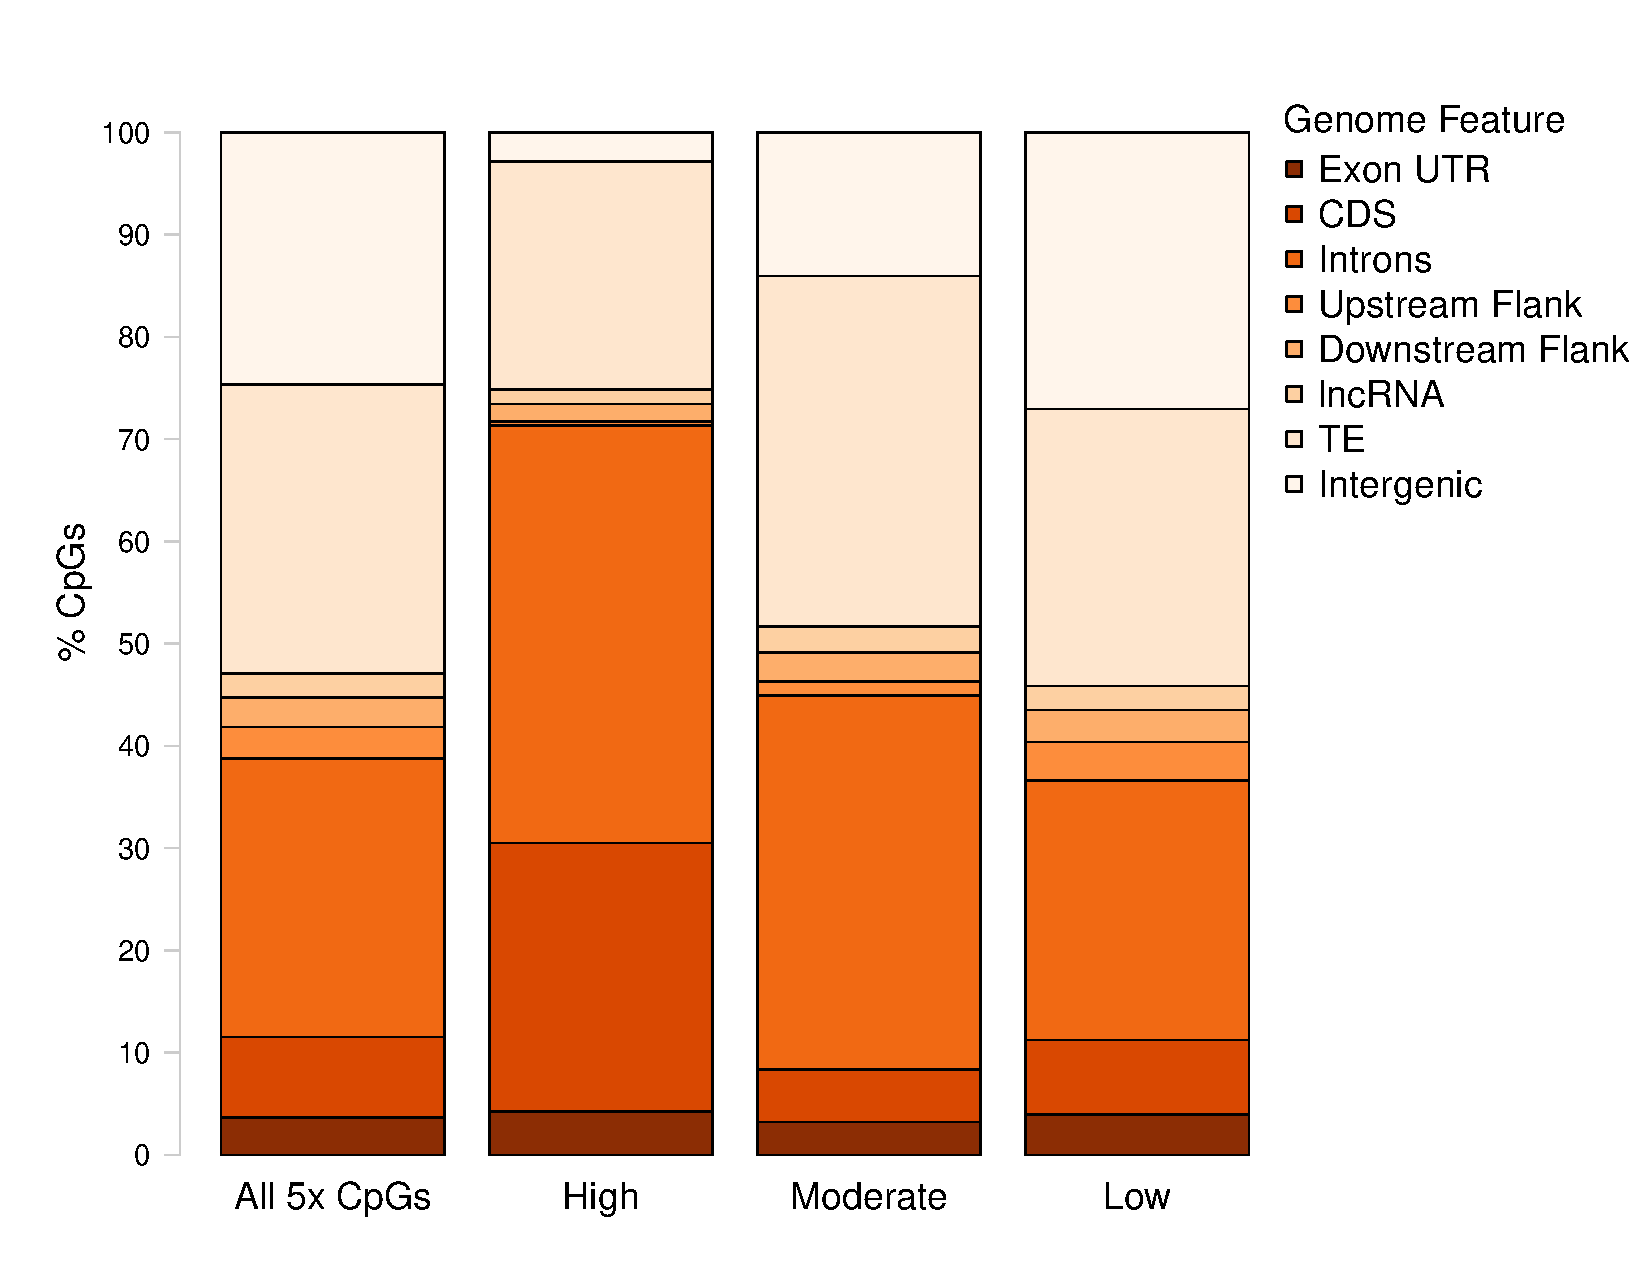
\includegraphics[width=1\textwidth]{figure/Ch3/Figure3.1.pdf}
  \caption{Genomic location of various CpG categories}
  \label{fig:fembackground}
\end{figure}
\clearpage

\textbf{Figure} \ref{fig:femheatmap}: Percent methylation values for DML created using an euclidean distance matrix. Samples in low pH conditions are represented by black, and samples in ambient pH conditions are represented by grey, with maturation stage along the bottom (0 = indeterminate, 3 = mature female). Darker colors indicate higher percent methylation, and a density plot depicts the distribution of percent methylation values for a panel. A total of 1599 DML were identified using a logistic regression, using a chi-squared test and 50\% methylation difference cut-off.\newline 
\begin{figure}[h]
\centering
  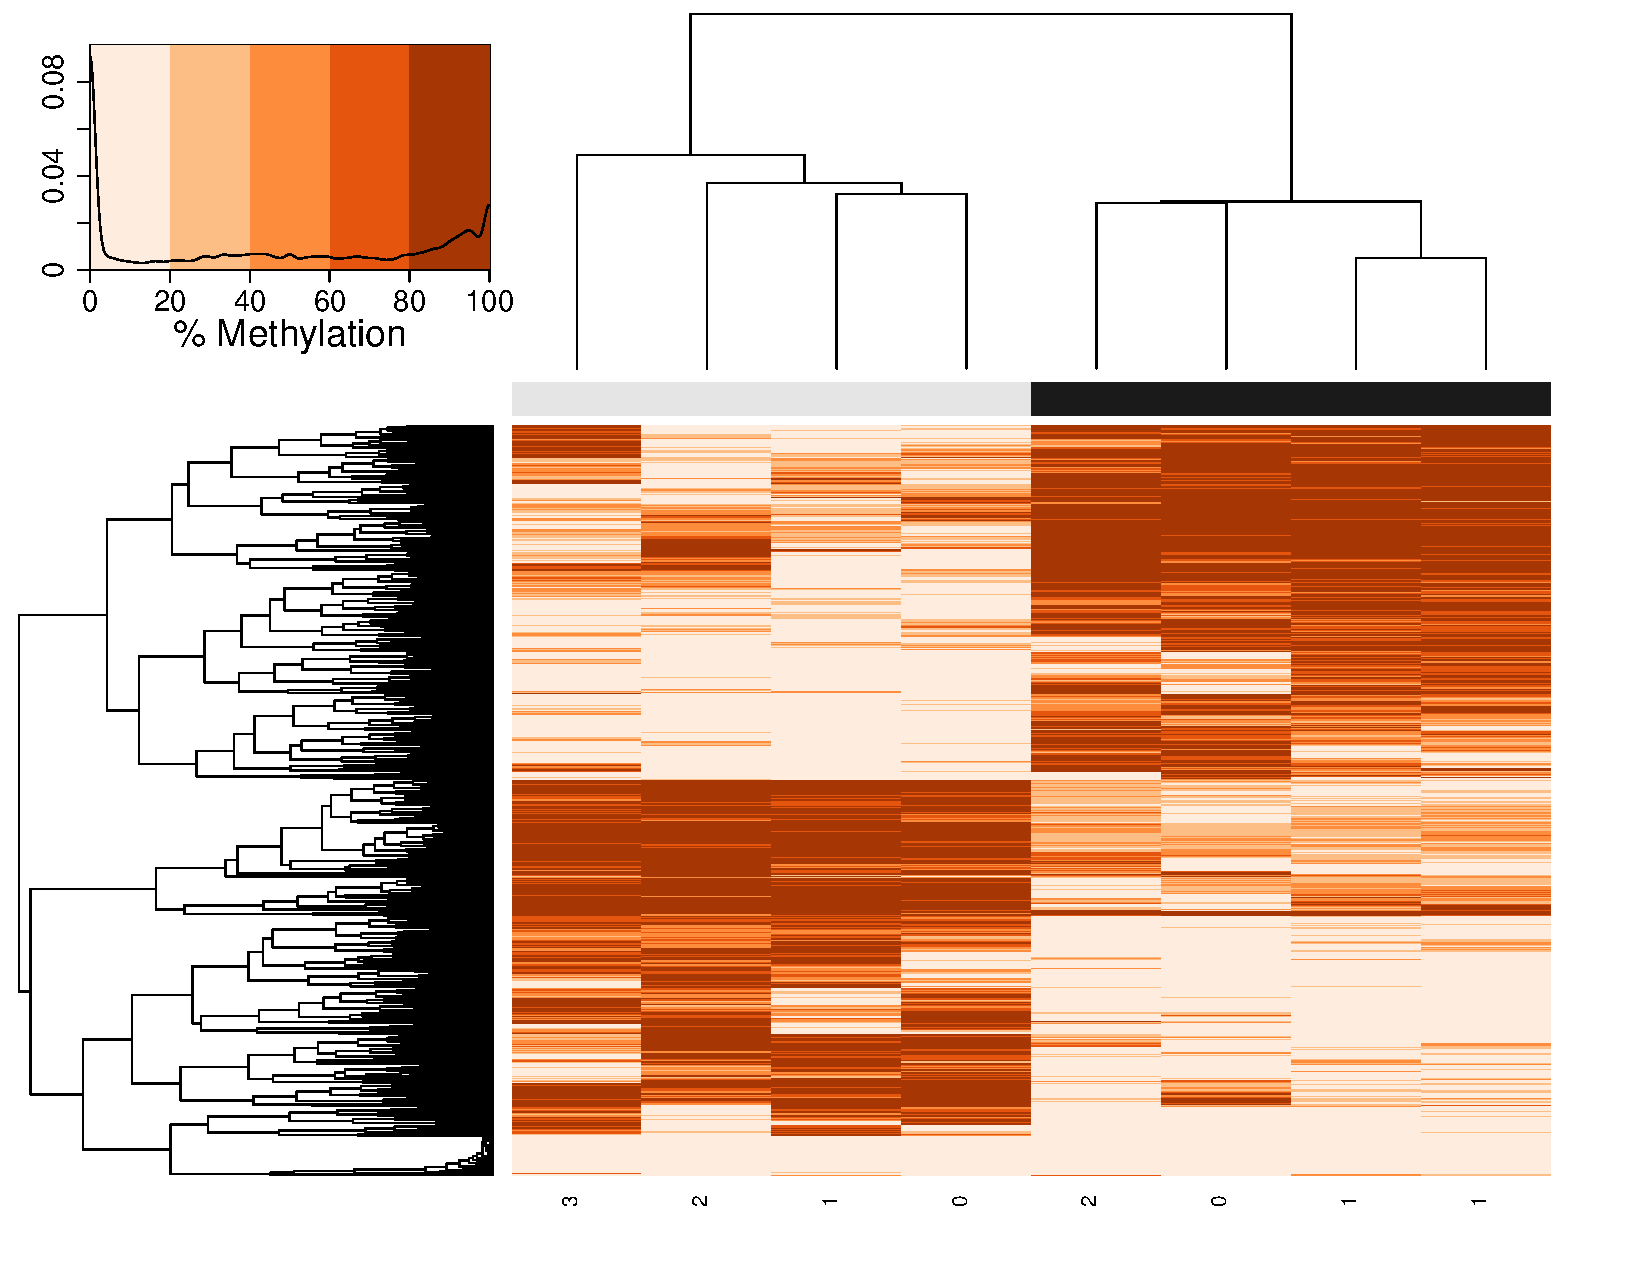
\includegraphics[width=1\textwidth]{figure/Ch3/Figure3.2.pdf}
  \caption{Heatmap of DML}
  \label{fig:femheatmap}
\end{figure}
\clearpage

\textbf{Figure} \ref{fig:chromdistr}: Number of DML normalized by number of CpG in each chromosome (bars) and number of genes (line) in each chromosome. Additional DML were identified in scaffolds that were not mapped to any of the ten main linkage groups.\newline 
\begin{figure}[h]
\centering
  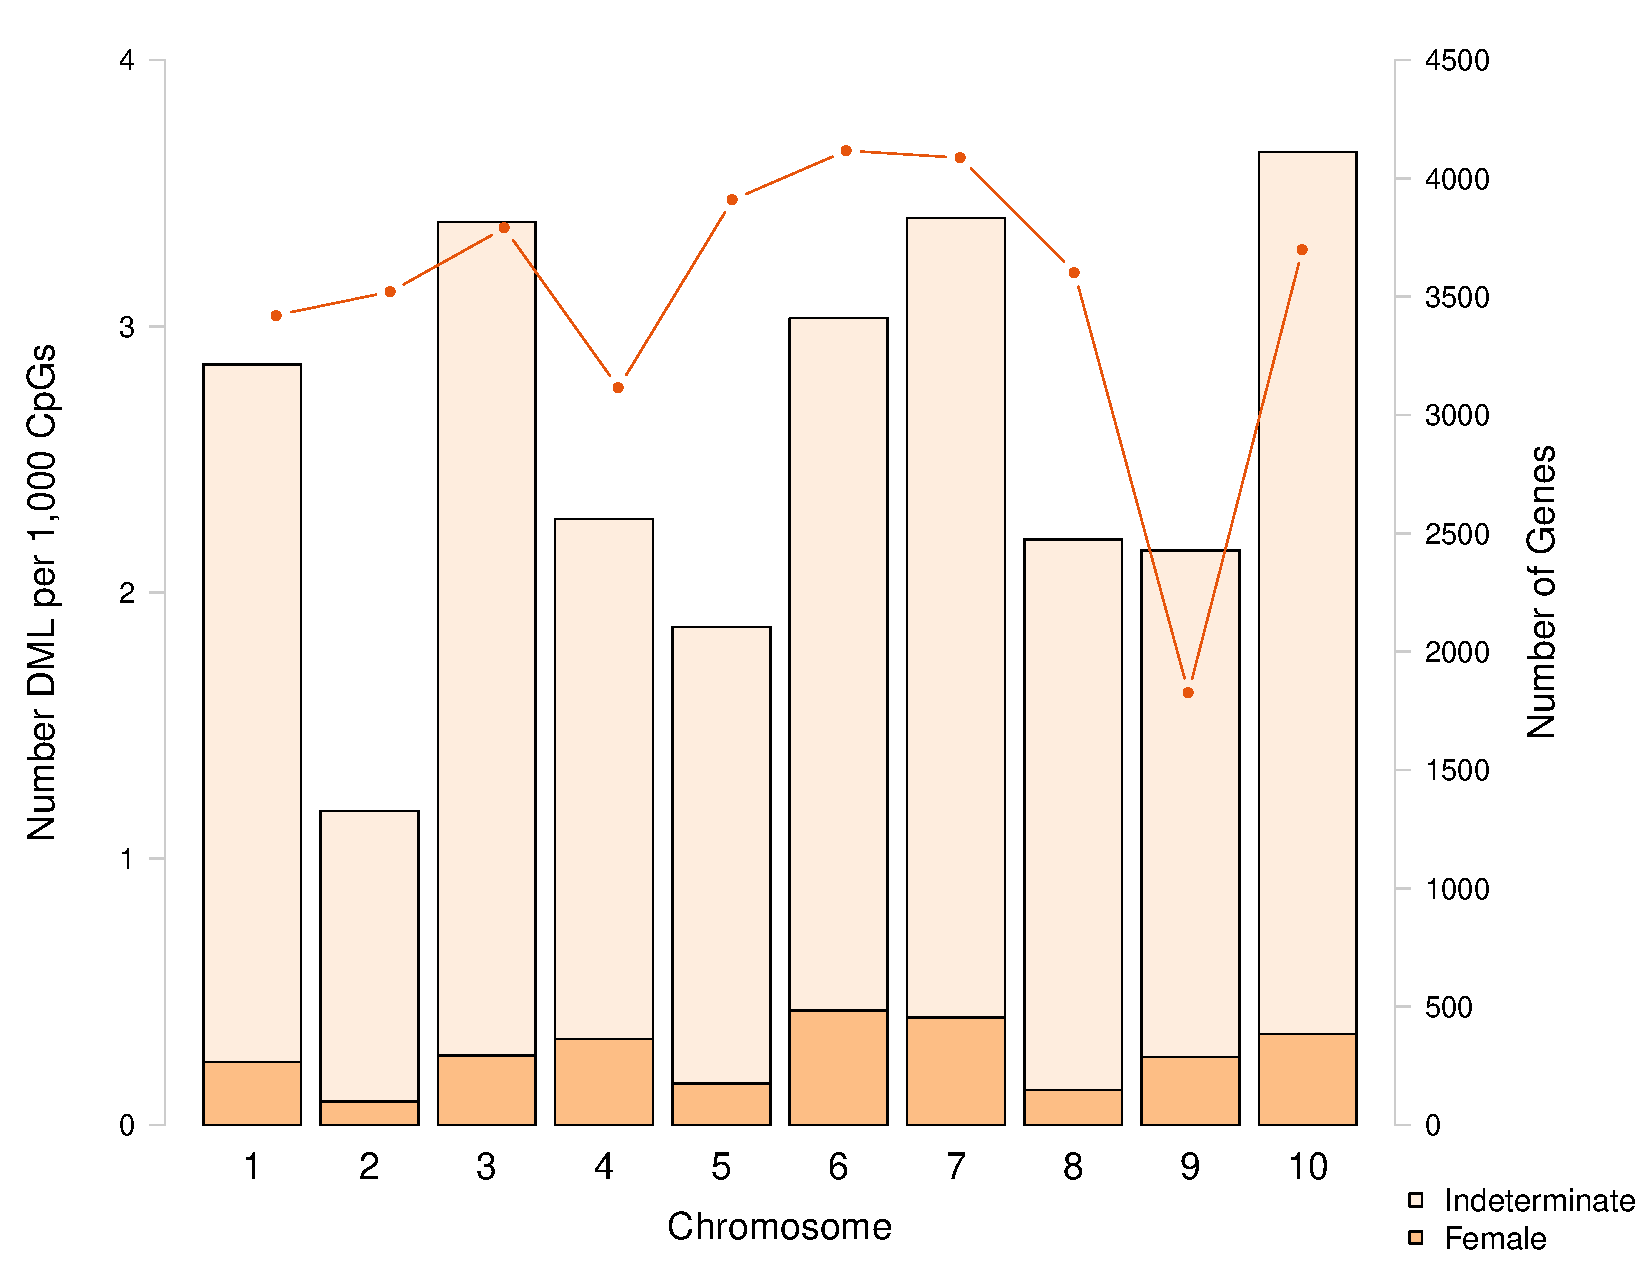
\includegraphics[width=1\textwidth]{figure/Ch3/Figure3.3.pdf}
  \caption{Distribution of DML in main chromosomes}
  \label{fig:chromdistr}
\end{figure}
\clearpage

\textbf{Figure} \ref{fig:locDML}: Distribution of all CpGs with 5x coverage and DML in various genome features.\newline 
\begin{figure}[h]
\centering
  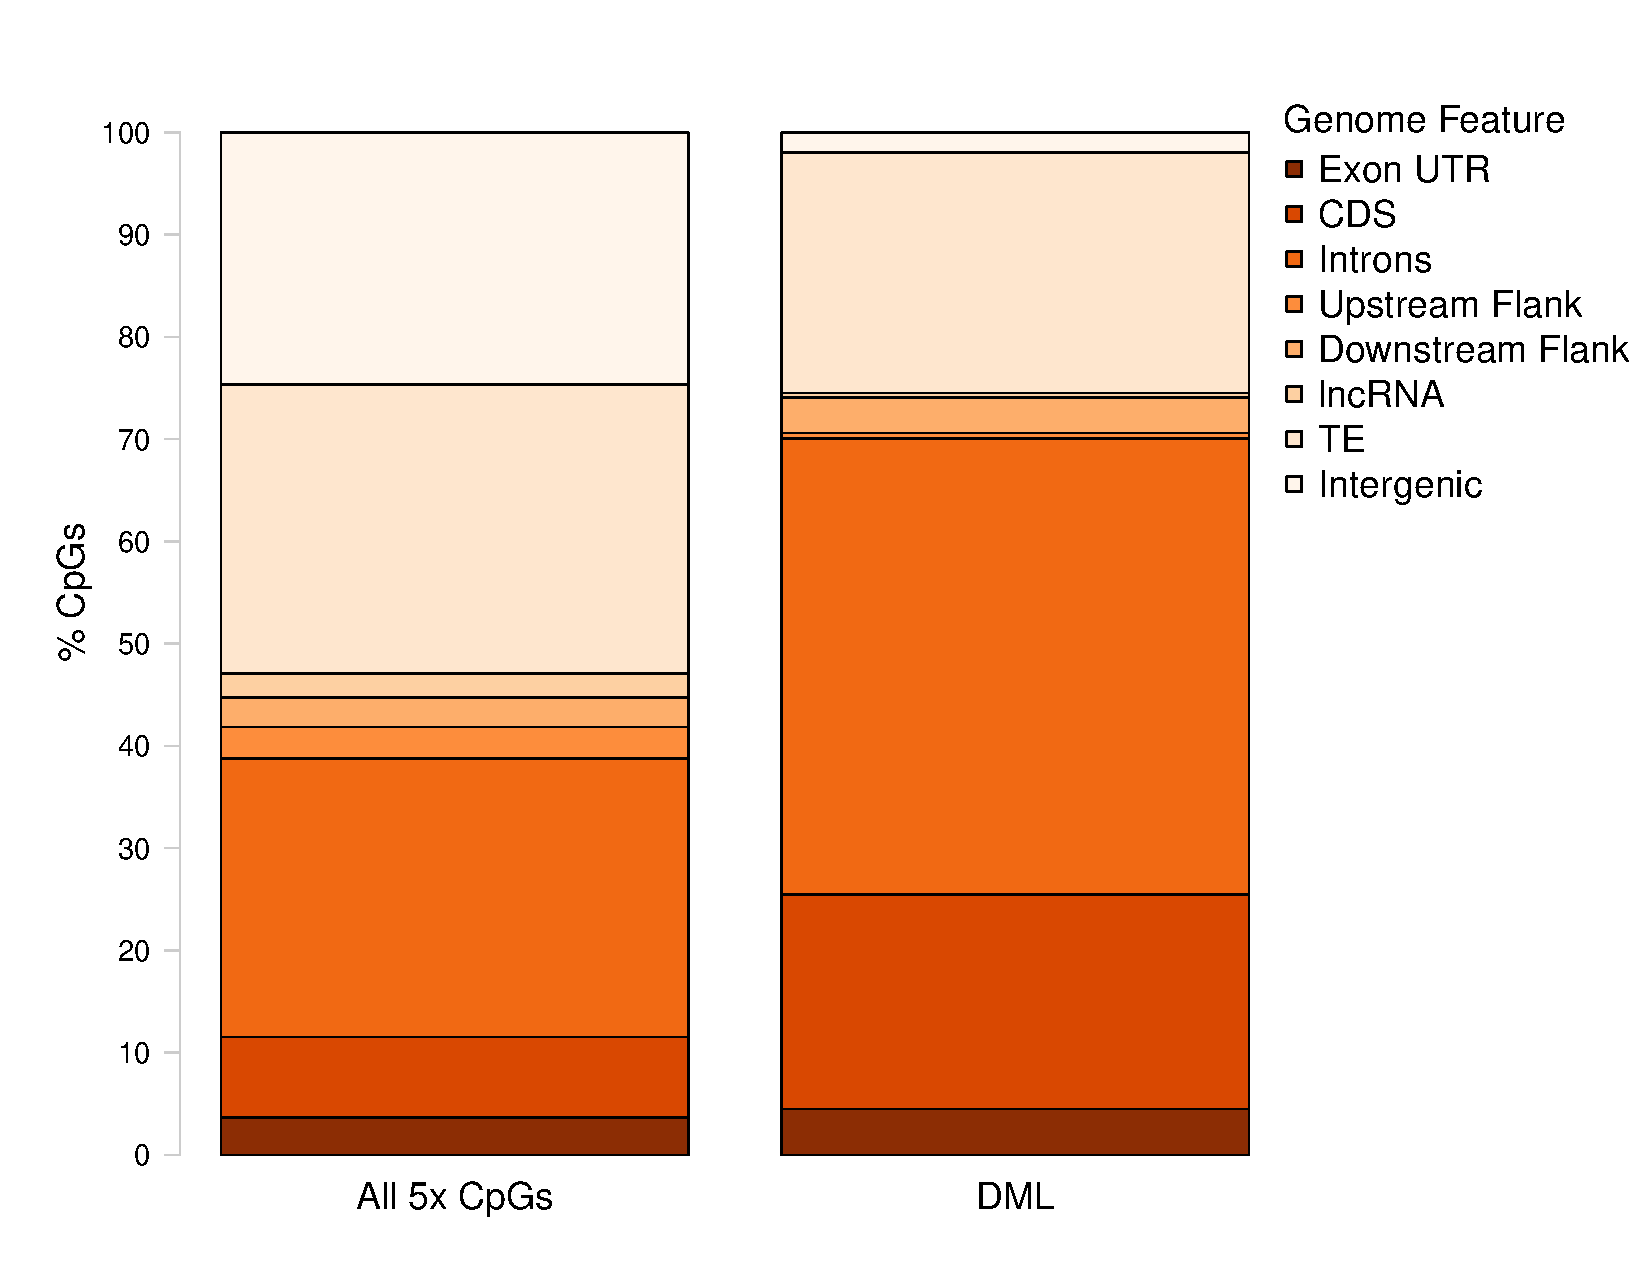
\includegraphics[width=1\textwidth]{figure/Ch3/Figure3.4.pdf}
  \caption{Genomic location of DML}
  \label{fig:locDML}
\end{figure}
\clearpage

\textbf{Figure} \ref{fig:simplifyEnrichment}: Biological process GOterms enriched in genes containing DML. A semantic similarity matrix was generated using ``Relevance'' measures, then clustered using the binary cut method. The GOterms associated with each cluster are displayed in the word cloud, with the size of the word representing frequency in the dataset. Darker colors represent GOterms that have higher semantic similarity.\newline 
\begin{figure}[h]
\centering
  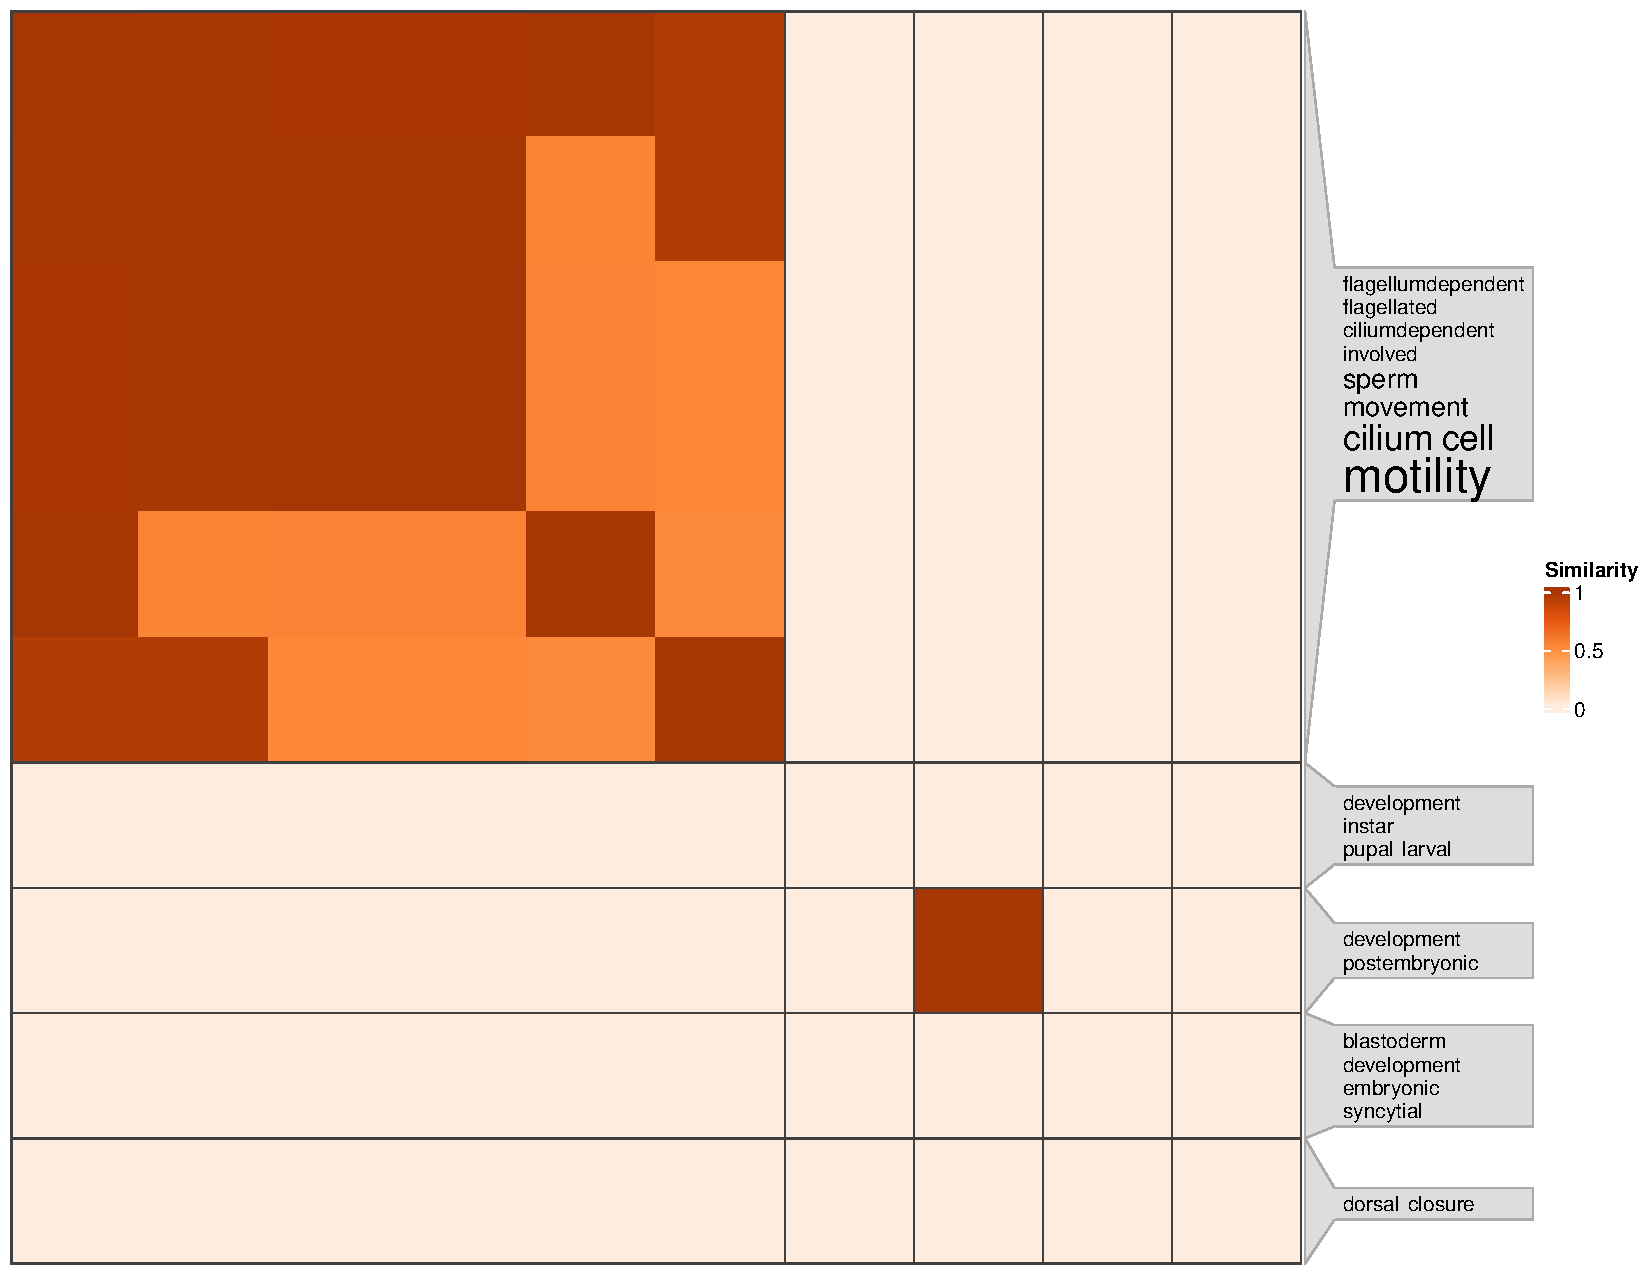
\includegraphics[width=1\textwidth]{figure/Ch3/Figure3.5.pdf}
  \caption{Significantly enriched GOterms}
  \label{fig:simplifyEnrichment}
\end{figure}
\clearpage

\hypertarget{polyploidy-and-environmental-stress-have-distinct-impacts-on-pacific-oyster-crassostrea-gigas-ctenidia-methylomes}{%
\chapter{\texorpdfstring{Polyploidy and environmental stress have distinct impacts on Pacific oyster (\emph{Crassostrea gigas}) ctenidia methylomes}{Polyploidy and environmental stress have distinct impacts on Pacific oyster (Crassostrea gigas) ctenidia methylomes}}\label{polyploidy-and-environmental-stress-have-distinct-impacts-on-pacific-oyster-crassostrea-gigas-ctenidia-methylomes}}

\hypertarget{abstract-3}{%
\section{Abstract}\label{abstract-3}}

Production of polyploid organisms resilient to environmental change requires a molecular understanding of stress response mechanisms. This is especially important when considering the use of triploid oysters in commercial aquaculture settings. Examination of DNA methylation can elucidate gene expression regulation mechanisms employed by triploid oysters, and how they may differ from their diploid counterparts. In other cultured marine organisms, polyploid induction does not yield methylation variation similar to organisms that undergo natural genome duplication. We examined how artificial genome duplication and environmental variation contribute to stress response phenotypes in the Pacific oyster (\emph{Crassostrea gigas}). We exposed diploid (n = 12) and triploid (n = 12) \emph{C. gigas} to low or high pH stress for six weeks. Ctenidia methylomes were then obtained using whole genome bisulfite sequencing. While there were no global methylation differences between samples, distinct differentially methylated loci (DML) were associated with ploidy status (154 ploidy-DML) and pH condition (178 pH-DML). Functions of genes containing ploidy-DML were not similar to those observed in organisms that undergo natural polyploidization. However, genes with pH-DML were associated with apoptosis, protein ubiquitination, zinc ion binding, and cytoskeletal processes commonly observed in oyster response to ocean acidification. Given the enrichment of both ploidy- and pH-DML in genes with multiple transcripts, it is possible that these methylation changes can influence gene expression and physiological phenotype. Our study --- which is the first to provide single base-pair resolution assessment of diploid and triploid methylomes in a marine invertebrate --- suggests that while methylation may play different regulatory roles during artificial and natural genome duplication events, environmentally-sensitive methylome responses may be uniform between diploid and triploid \emph{C. gigas}.

\hypertarget{introduction-4}{%
\section{Introduction}\label{introduction-4}}

As molluscan breeding programs focus on developing oyster lines resilient to environmental stressors associated with climate change, several programs are focusing on culturing triploid organisms. Triploid oysters, which may be generated through chemical induction or by mating diploid and tetraploid parents, contain three copies of the genome (\protect\hyperlink{ref-Nell2002}{Nell, 2002}). This third genome copy renders these oysters partially sterile, with triploids diverting resources that would be for reproduction towards growth (\protect\hyperlink{ref-Nell2002}{Nell, 2002}). As a result, triploids exhibit significantly faster growth rates, improved meat quality, and increased survival, with mated triploids having an additional advantage over chemically-induced oysters (\protect\hyperlink{ref-Wadsworth2019}{Wadsworth, Wilson, \& Walton, 2019}). The potential advantages of triploidy have been examined with respect to heat stress, salinity, hypoxia, and disease pressure in \emph{Crassostrea spp}. While triploid Pacific oysters (\emph{Crassostrea gigas}) may have an energetic advantage over their diploid counterparts at elevated temperatures due to reduced gonadal investment and corresponding increases in tissue weight, condition index, protein, and carbohydrate levels (\protect\hyperlink{ref-Shpigel1992}{Shpigel, Barber, \& Mann, 1992}), triploid eastern oysters (\emph{C. virginica}) are more sensitive to desiccation stress associated with farm rearing, and display higher mortality than their diploid counterparts (\protect\hyperlink{ref-Bodenstein2021}{Bodenstein, Walton, \& Steury, 2021}). Triploid hybrids of the edible oyster \emph{Crassostrea hongkongensis} and Suminoe oyster \emph{Crassostrea ariakensis} grew faster as larvae in the hatchery and as juveniles in environmentally-distinct outplant locations, but displayed less salinity tolerance than their diploid hybrid counterparts (\protect\hyperlink{ref-Qin2020}{Qin et al., 2020}). Low salinity conditions in the Chesapeake Bay removed growth advantages associated with \emph{C. virginica} triploids (\protect\hyperlink{ref-Callam2016}{Callam, Allen, \& Frank-Lawale, 2016}). While triploid \emph{C. virginica} juveniles did not display any survival differences in hypoxic conditions, time to mortality in \emph{C. ariakensis} triploids was three times earlier than diploid oysters (\protect\hyperlink{ref-Lombardi2013}{Lombardi, Harlan, \& Paynter, 2013}). Active gametogenesis in \emph{C. gigas} lead to increased \emph{Vibrio} infection, irrespective of ploidy status, but triploid oysters had poorer survival after disease challenges in winter conditions (\protect\hyperlink{ref-DeDecker2011}{De Decker et al., 2011}). In the Chesapeake Bay, triploid \emph{C. virginica} had lower mortality and greater shell height, weight, yield, and a higher proportion of market-sized oysters than diploids, even when faced with similar \emph{Perkinsus marinus} disease pressure (\protect\hyperlink{ref-Degremont2012}{Dégremont, Garcia, Frank-Lawale, \& Allen, 2012}). However, triploid \emph{C. virginica} were susceptible to mortality events that are not associated with disease or environmental conditions, suggesting that there are elements of triploid physiology and stress response still unknown (\protect\hyperlink{ref-Matt2020}{Matt, Guévélou, Small, \& Allen, 2020}). To date, there is no documentation of triploid oyster responses to ocean acidification, and how this stress response differs from diploid organisms. Even though triploids are more sensitive to a variety of environmental stressors, without a mechanistic understanding of triploid sensitivity to ocean acidification, it is difficult to implement hatchery techniques such as environmental manipulation to produce more stress-tolerant triploid phenotypes (\protect\hyperlink{ref-Gavery2017}{Gavery \& Roberts, 2017}).

Epigenetic mechanisms, like DNA methylation, can mediate phenotypic plasticity and responses to environmental stressors, which makes them useful for understanding triploid stress tolerance. Epigenetics refers to changes in gene expression that do not arise from changes in the DNA sequence, with methylation of cytosine bases being the most studied mechanism (\protect\hyperlink{ref-Bird2002}{Bird, 2002}; \protect\hyperlink{ref-Deans2015}{Deans \& Maggert, 2015}). Baseline variation in methylation patterns, or standing epigenetic variation, can be associated with genomic structure. Currently, polyploidization impacts on DNA methylation is well-understood in organisms that demonstrate natural ploidy variation. Genome duplication events in plants are subsequently followed by sequence loss, gene duplication, transposon silencing, and changes to genome regulation mediated by epigenetic mechanisms (\protect\hyperlink{ref-Adams2005}{Adams \& Wendel, 2005}; \protect\hyperlink{ref-Chen2006}{Chen \& Ni, 2006}; \protect\hyperlink{ref-Henry2005}{Henry, 2005}; \protect\hyperlink{ref-Matzke1999}{Matzke, Mittelsten Scheid, \& Matzke, 1999}; \protect\hyperlink{ref-Salmon2005}{Salmon, Ainouche, \& Wendel, 2005}; \protect\hyperlink{ref-Verhoeven2010}{Verhoeven, Van Dijk, \& Biere, 2010}; \protect\hyperlink{ref-Wang2004}{J. Wang et al., 2004}). These methylation changes promote normal genomic function after polyploidization, and can persist for a few generations after the duplication event (\protect\hyperlink{ref-Wang2004}{J. Wang et al., 2004}). Social insects with natural genome duplication also display distinct methylation variation associated predominantly with ploidy status, which may be responsible for reducing transcriptional noise in haploid organisms (\protect\hyperlink{ref-Glastad2014}{Glastad, Hunt, Yi, \& Goodisman, 2014}). Organisms that experience induced triploidy may not display methylation variation associated with genome duplication. For example, examination of diploid and artificially-induced \emph{C. gigas} and brown trout (\emph{Salmo trutta} L.) did not find any global methylation differences (\protect\hyperlink{ref-Covelo-Soto2015}{Covelo-Soto, Leunda, Pérez-Figueroa, \& Morán, 2015}; \protect\hyperlink{ref-Jiang2016}{Jiang, Li, Yu, \& Kong, 2016}). Even so, promoter sequences in triploid \emph{Apostichopus japonicus} sea cucumbers exhibited correlation between methylation and expression (\protect\hyperlink{ref-Han2021}{Han et al., 2021}). As standing methylation can still influence gene expression in triploid organisms, investigating these mechanisms can provide insight into triploid oyster gene expression regulation.

Ocean acidification, can also influence methylomes (\protect\hyperlink{ref-Eirin-Lopez2018}{Eirin-Lopez \& Putnam, 2018}), with pteropods (\protect\hyperlink{ref-Bogan2020}{Bogan, Johnson, \& Hofmann, 2020}), corals (\protect\hyperlink{ref-Liew2018b}{Liew, Zoccola, et al., 2018}; \protect\hyperlink{ref-Putnam2016}{Putnam, Davidson, \& Gates, 2016}), and urchins (\protect\hyperlink{ref-Strader2020}{Marie E. Strader et al., 2020}; \protect\hyperlink{ref-Strader2019}{M. E. Strader, Wong, Kozal, Leach, \& Hofmann, 2019}) demonstrating distinct methylation patterns in response to low pH. Diploid oysters have been well-studied in this respect. Eastern oyster (\emph{C. virginica}) mantle (\protect\hyperlink{ref-Downey-Wall2020}{Downey-Wall et al., 2020}) and gonad (\protect\hyperlink{ref-Venkataraman2020}{Venkataraman et al., 2020}), and \emph{C. hongkongensis} mantle (\protect\hyperlink{ref-ChandraRajan2021}{Chandra Rajan, Yuan, Yu, Roberts, \& Thiyagarajan, 2021}), and larvae (\protect\hyperlink{ref-Lim2020}{Lim et al., 2020}) all display changes in DNA methylation after experimental ocean acidification exposure. However, no studies to date have examined environmentally-sensitive methylation in triploids. In plants, polyploidization can influence the standing methylation variation that evolves over time and interacts with environmental stressors (\protect\hyperlink{ref-Verhoeven2010}{Verhoeven, Van Dijk, \& Biere, 2010}). Transcriptomic investigations have started to unveil differences in diploid and triploid stress responses in molluscan species. For example, triploid abalone exposed to heat stress and hypoxia conditions exhibited significantly different transcriptional changes when compared to diploids (\protect\hyperlink{ref-Kim2021}{Kim, Kim, Seo, Park, \& Nam, 2021}). Since DNA methylation could influence gene activity and impact stress responses, elucidating genomic and environmental variation contribute to phenotype is crucial for understanding potential acclimatization mechanisms and their application to triploid aquaculture (\protect\hyperlink{ref-Gavery2017}{Gavery \& Roberts, 2017}).

We present the first single-base pair resolution examination of diploid and triploid \emph{C. gigas} methylomes in response to an environmental stressor. Our comparison of DNA methylation by ploidy status allows us to discern how epigenetic variation differs with genome duplication. By comparing oyster methylomes exposed to low and high pH conditions, we can elucidate how ocean acidification can exert an influence over ctenidia methylation. Finally, we determine if genetic and environmental variation interact to produce a unique methylation phenotype. Our work provides the foundation for understanding the mechanisms behind triploid \emph{C. gigas} stress responses, and the application of knowledge for aquaculture practices that select for oysters resilient to climate stressors.

\hypertarget{methods-3}{%
\section{Methods}\label{methods-3}}

\hypertarget{experimental-design-1}{%
\subsection{Experimental Design}\label{experimental-design-1}}

Pacific oysters (n = 24) were obtained from the Hawaiian Shellfish LLC hatchery located in Kea`au, Hawaiʻi Island and held at the University of Hawai'i, Hilo. The broodstock used to produce these oysters originated from the Molluscan Broodstock Program at Oregon State University. Triploids were produced by mating diploid female and tetraploid male oysters. The diploids used in the experiment were not used to produce the triploids. Diploid (n = 12) and triploid (n = 12) \emph{C. gigas} were randomly assigned to each of two treatments (high pH and low pH).

The treatment tanks were 150 gallon conical bottom tanks with flow-through seawater from a deep well. Carbon dioxide was dispersed into both treatment tanks to achieve ``non-acidification'' conditions (pCO\textsubscript{2} ranged from 67.37 to 98.61 µatm) to ``ocean acidification'' conditions (pCO\textsubscript{2} ranged from 287.88 to 418.20 µatm). Water quality parameters were checked daily. pH probes were placed about 2.5 cm under the surface of the water and connected to pH controllers (American Marine). Dissolved oxygen, salinity, and temperature were monitored daily with an YSI Pro 2030. Ammonia concentration was monitored daily using an aquarium test kit (API). Full water exchanges were performed daily. Since the ctenidia is the primary tissue that interacts with the environment, ctenidia tissue was obtained from each oyster after six weeks, preserved in 2 mL DNA/RNA Shield (ZymoResearch), then stored at -20ºC.

\hypertarget{dna-extraction-and-library-preparation-1}{%
\subsection{DNA Extraction and Library Preparation}\label{dna-extraction-and-library-preparation-1}}

DNA was extracted from each sample for Whole Genome Bisulfite Sequencing (WGBS). Samples were centrifuged for one minute at 10,000 RCF to pellet ctenidia tissue. After removing the DNA/RNA shield, ctenidia DNA was extracted using the E.Z.N.A. Mollusc Kit (Omega). Manufacturer's protocol was followed, with the exception of an overnight incubation at 37ºC after the addition of 350 µL ML1 Buffer and 25 µL Proteinase K Solution. After the MB1 lysis buffer was added to samples, a thick white precipitate formed. Samples were vortexed to emulsify the precipitate, but several samples did not lyse fully. Samples were eluted with 100 µL of Elution Buffer. A Qubit™ 3.0 and dsDNA BR Assay (Invitrogen) was used to confirm that samples contained at least 500 ng of DNA, using 2 µL of DNA for each sample.

Samples were sent to ZymoResearch for bisulfite conversion and library preparation. Bisulfite conversion was performed with the Pico Methyl-Seq Library Prep Kit (Cat. \#D5455). Per ZymoResearch protocol, samples were spiked with a mixture of six unique double-stranded synthetic amplicons (180-200 bp) from the \emph{Escherichia coli} K12 genome. Since each amplicon represents a different percent methylation, the spike-in was used to determine bisulfite conversion efficiency. Libraries were barcoded and pooled into a single lane to generate 150 bp paired-end reads in a single Illumina NovaSeq flowcell.

\hypertarget{genome-information-and-feature-tracks-1}{%
\subsection{Genome Information and Feature Tracks}\label{genome-information-and-feature-tracks-1}}

Nuclear (\protect\hyperlink{ref-Penaloza2021}{Peñaloza et al., 2021}) (NCBI GenBank: GCA\_902806645.1, RefSeq: GCF\_902806645.1) and mitochondrial genome sequences (NCBI Reference Sequence: NC\_001276.1) were used in downstream analysis. These sequences were combined for downstream alignment. The \texttt{fuzznuc} function within EMBOSS was used to identify CG motifs in the combined nuclear and mitochondrial sequences.

The RefSeq annotation was used to obtain genome feature tracks, and create additional tracks. The annotation included a combination of Gnomon, RefSeq, cmsearch, and tRNAscan-SE predictions. Gene, coding sequence, exon, and lncRNA tracks were extracted from the RefSeq annotation. These tracks were then used to obtain additional genome feature information. To create an intron track, the complement of the exon track was generated with BEDtools \texttt{complementBed} v.2.26.0 to create a non-coding sequence track (\protect\hyperlink{ref-Quinlan2010}{Quinlan \& Hall, 2010}). The overlap between the genes and the non-coding sequences was found with \texttt{intersectBed} and defined as introns. Similarly, untranslated regions of exons were obtained by subtracting coding sequences from exon information with \texttt{subtractBed}. Flanking regions were defined as the 1000 bp upstream or downstream of genes. Upstream flanks were generated by adding 1000 bp upstream of genes, taking into account strand, with \texttt{flankBed}. Existing genes were removed from flanking sequences using \texttt{subtractBed}. A similar process was performed to generate downstream flanking regions. Intergenic regions were isolated by finding the complement of genes with \texttt{complementBed}, then using \texttt{subtractBed} to remove any flanks. Transposable element locations were obtained from RepeatMasker using the NCBI RefSeq annotation (RefSeq: GCF\_902806645.1) (\protect\hyperlink{ref-Smit2013}{Smit, Hubley, \& Green, 2013}; \protect\hyperlink{ref-Tarailo-Graovac2009}{Tarailo-Graovac \& Chen, 2009}). The number of CG motifs in a genome track was obtained using \texttt{intersectBed}.

\hypertarget{sequence-alignment-2}{%
\subsection{Sequence Alignment}\label{sequence-alignment-2}}

Prior to alignment, 150 bp paired-end reads generated for each sample underwent three rounds of trimming. First, Illumina adapter sequences were removed from samples using TrimGalore! v.0.6.6 (\protect\hyperlink{ref-Martin2011}{Martin, 2011}). Additionally, 10 bp were trimmed from both the 5' (\texttt{-\/-clip\_R1\ 10} and \texttt{-\/-clip\_R2\ 10}) and 3' ends of paired reads (\texttt{-\/-three\_prime\_clip\_R1\ 10} and \texttt{-\/-three\_prime\_clip\_R2\ 10}). Remaining adapters were then removed from sequences in the second round of TrimGalore! trimming. Poly-G tails present in data were removed by manually specifying a matching adapter sequence (\texttt{-\/-adapter\ GGGGGGGGGGGGGGGGGGGGGGGGGGGGGGGGGGGGGGGGGGGGGGGGGG} and \texttt{-\/-adapter2\ GGGGGGGGGGGGGGGGGGGGGGGGGGGGGGGGGGGGGGGGGGGGGGGGGG}). After each round of trimming, sequence quality was assessed using FastQC v.0.11.9 (\protect\hyperlink{ref-Andrews2010}{Andrews, 2010}) and MultiQC reports (\protect\hyperlink{ref-Ewels2016}{Ewels, Magnusson, Lundin, \& Käller, 2016}).

Trimmed samples were then aligned to the \emph{C. gigas} genome (\protect\hyperlink{ref-Penaloza2021}{Peñaloza et al., 2021}). The full genome was bisulfite converted with Bowtie 2-2.3.4 (Linux x84\_64 version (\protect\hyperlink{ref-Langmead2012}{Langmead \& Salzberg, 2012})) using the \texttt{bismark\_genome\_preparation} function within Bismark v.0.22.3 (Krueger \& Andrews, 2011) prior to sequence alignment. Reads were then aligned to each bisulfite-converted genome, specifying non-directional input (\texttt{-\/-non\_directional}) and allowing for an alignment score no lower than -90 (\texttt{-score\_min\ L,0,-0.6}). Aligned BAM files were deduplicated with the \texttt{-\/-deduplicate\_bismark} function, then sorted and indexed for downstream applications using SAMtools v.1.10 (\protect\hyperlink{ref-Li2009}{Li et al., 2009}). Sequence methylation calls were extracted from deduplicated BAM files with \texttt{bismark\_methylation\_extractor}. Coverage files generated from methylation extraction contained CpG information from both strands. To consolidate CpG information between strands and report 1-based chromosomal coordinates for each CpG, \texttt{coverage2cytosine} was run on deduplicated coverage files. Using \texttt{coverage2cytosine} coverage file output, genomic coordinates for CpGs with at least 5x coverage across all samples were written to BEDgraphs. Finally, \texttt{bismark2report} and \texttt{bismark2summary} were used to create summary reports with alignment information for each sample that were concatenated with MultiQC.

\hypertarget{snp-identification-2}{%
\subsection{SNP Identification}\label{snp-identification-2}}

As genomic differences can play a role in methylation, single nucleotide polymorphisms (SNPs) were identified from WGBS data. Two methods were used for SNP identification. First, SNP variants across all samples and in individuals were identified with BS-Snper (\protect\hyperlink{ref-Gao2015}{Gao et al., 2015}). As \texttt{BS-Snper} only takes one input file, deduplicated and sorted BAM alignments generated with Bismark v.0.22.3 and SAMtools v.1.10 (\protect\hyperlink{ref-Krueger2011}{Krueger \& Andrews, 2011}; \protect\hyperlink{ref-Li2009}{Li et al., 2009}) were merged (\texttt{samtools\ merge}). Variants were then identified in the merged BAM file or individual deduplicated and sorted BAM files. Default \texttt{BS-Snper} settings were used, except for a minimum coverage of 5x to be consistent with methylation analyses. C/T SNPs were filtered by identifying overlaps (\texttt{intersectBED}) between each set of SNPs and the CG motif track.

\hypertarget{global-methylation-characterization-1}{%
\subsection{Global Methylation Characterization}\label{global-methylation-characterization-1}}

Global methylation patterns were characterized using CpG loci with at least 5x coverage in all samples. BEDgraphs produced with Bismark v.0.22.3 were sorted (\texttt{sortBed}), then used to concatenate percent methylation information across samples (\texttt{unionBedGraphs}). Percent methylation values were averaged between all samples for each CpG locus. These loci were categorized as highly (≥ 50\%), moderately (10-50\%), or lowly methylated (≤10\%) based on average percent methylation values. The genomic location of these methylation categories was determined with respect to UTR, CDS, introns, up- and downstream flanking regions, transposable elements, and intergenic regions (\texttt{intersectBed}). We tested the null hypothesis that there was no association between the genomic location of CpG loci and methylation status (all CpGs versus highly methylated CpGs) with a chi-squared contingency test (\texttt{chisq.test} in R Version 3.5.3 (\protect\hyperlink{ref-R_Core_Team2019}{R Core Team, 2019})). To quantify differences in percent methylation by ploidy status, percent methylation values from the union BEDgraph were averaged for diploid and triploid samples separately.

As methylation detection relies on coverage, we also estimated average coverage for diploid and triploid oysters. Merged coverage files produced with Bismark v.0.22.3 were sorted (\texttt{sortBed}), then used to concatenate coverage information across samples (\texttt{unionBedGraphs}). Coverage was averaged for diploid and triploid samples separately to quantify if ploidy status influenced coverage.

Methylation patterns were compared between treatments using \texttt{methylKit} v.1.17.4 (\protect\hyperlink{ref-Akalin2012}{Akalin et al., 2012}) with R Version 3.5.3 (\protect\hyperlink{ref-R_Core_Team2019}{R Core Team, 2019}). Data with at least 2x coverage from merged CpG coverage files produced by \texttt{coverage2cytosine} were imported using \texttt{methRead.} For each sample, data was filtered further (\texttt{filterByCoverage}) by requiring at least 5x coverage for each CpG (\texttt{lo.count\ =\ 5}), and removing potential PCR duplicates by excluding data in the 99.9th percentile of coverage (\texttt{high.perc\ =\ 99.9}). Filtered data were then normalized (\texttt{normalizeCoverage}) between samples to avoid over-sampling reads from one sample during downstream statistical analysis. Percent methylation (\texttt{getMethylationStats}) and CpG coverage (\texttt{getCoverageStats}) histograms were generated for each sample to confirm normalization. Filtered and normalized data were combined (unite) for every CpG position with at least 5x coverage with data in at least eight samples per treatment to generate a CpG background. Pairwise Pearson's correlation coefficients were calculated and a global Principal Component Analysis based on percent methylation profiles was conducted to understand similarities and differences in sample methylation.

\hypertarget{identification-of-differentially-methylated-loci-1}{%
\subsection{Identification of Differentially Methylated Loci}\label{identification-of-differentially-methylated-loci-1}}

Differentially methylated loci (DML) were identified using a generalized experimental design with \texttt{DSS} v.2.38.0 (Feng et al., 2014). The purpose of this generalized design was to test pH, ploidy, and their interaction simultaneously. For each sample, the corresponding merged coverage file from Bismark v.0.22.3 were modified to meet DSS input formatting requirements. The coverage file contained information for CpG loci with at least 1x coverage in that sample. Only the start position in the coverage files was used, and the number of total reads was calculated by summing the number of methylated and unmethylated reads provided in the coverage files. The final input files included the following columns: chromosome, start position, number of total reads, and number of methylated reads. Data was not pre-filtered based on a coverage threshold, following DSS input specifications. After importing information into R Studio using \texttt{list2env}, a BSseq object (\texttt{makeBSseqData}, \texttt{bsseq} v.1.26.0) was generated with coverage data to use for model fitting. To define the experimental design, a data frame was created with ploidy status (``D'' = diploid vs.~``T'' = triploid), pH treatment (``H'' = high pH vs.~``L'' = low pH), and sample ID.

Methylation was calculated at each CpG locus using the Bayesian hierarchical model framework provided by \texttt{DSS.} Coverage data were modeled using a beta-binomial distribution with an arcsine link function and log-normal priors (\protect\hyperlink{ref-Feng2014}{Feng, Conneely, \& Wu, 2014}). Unlike the Fisher's exact test used by \texttt{methylKit}, \texttt{DSS} assumes that data from each sample do not have identical distributions, retaining biological variation between samples in a treatment. The model was fitted onto transformed data using the generalized least squares method, defining pH, ploidy, and their interaction as coefficients (\texttt{DMLfit.multiFactor,\ formula\ =\ \textasciitilde{}\ ploidy\ +\ pH\ +\ ploidy:pH}). Smoothing, or using information from nearby CpG sites to inform methylation calculations, was not used, as invertebrate methylation data does not tend to be dense enough to provide multiple CpG dinucleotides in close proximity to each other.

A Wald test (\texttt{DMLtest.multiFactor}) was used at each CpG site for statistical testing of differential methylation for each coefficient separately (\texttt{ploidyT}, \texttt{pHL}, \texttt{ploidyT:pHL}). The test itself depends on sequencing depth, and a dispersion parameter defined by a shrinkage estimator from the Bayesian hierarchical model. The DML (ploidy-DML, pH-DML, and interaction-DML) were defined based on a P-value \textless{} 0.05 and Benjamini-Hochberg FDR \textless{} 0.01. The multiple regression framework used does not provide methylation values, so percent methylation differences were not used to define DML from \texttt{DSS.} BEDfiles with DML information were created for downstream analysis and visualized with sample coverage information using Integrative Genomics Viewer (IGV) version 2.9.2 (\protect\hyperlink{ref-Thorvaldsdottir2013}{Thorvaldsdóttir, Robinson, \& Mesirov, 2013}).

\hypertarget{dml-characterization-2}{%
\subsection{DML Characterization}\label{dml-characterization-2}}

Overlaps between all DML BEDfiles and UTR, CDS, introns, up- and downstream flanks, transposable elements, and intergenic regions (\texttt{intersectBed}) were used to describe where DML were located in the \emph{C. gigas} genome. A chi-squared contingency test was used to test the null hypothesis of no association between methylation and specific genome features using all CpGs with 5x data and DML. The number of DML in each chromosome was quantified and divided by chromosome length to discern if DML were distributed uniformly across the genome.

To determine if ploidy and pH treatments elicited similar methylation responses, we identified loci common between pH-DML, ploidy-DML, and interaction-DML. Overlaps between these lists were obtained using intersectBed. Additionally, overlaps between C/T SNPs and DML were also identified to discern if genomic factors other than treatment contributed to methylation responses.

\hypertarget{functional-enrichment-analysis}{%
\subsection{Functional Enrichment Analysis}\label{functional-enrichment-analysis}}

A functional enrichment analysis was performed to identify gene ontology (GO) terms significantly overrepresented in genes with ploidy-, pH-, or interaction-DML. Prior to enrichment, a blastx was performed against the Uniprot-SwissProt database (accessed June 01, 2021) (\protect\hyperlink{ref-UniProt_Consortium2019}{UniProt Consortium, 2019}) to obtain Uniprot Accession information for each RNA nucleotide sequence from the genome (GCF\_902806645.1\_cgigas\_uk\_roslin\_v1\_rna\_from\_genomic.fna available in the NCBI Annotation Release 102). The Uniprot Accession codes were used to match transcript IDs from the blastx output with GO terms from the Uniprot-Swissprot database.

Gene enrichment analysis was conducted with \texttt{topGO} v.2.34.0 in R (\protect\hyperlink{ref-Alexa2010}{Alexa, Rahnenfuhrer, \& Others, 2010}). First, a gene ID-to-GO term database (\texttt{geneID2GO}) was created for manual GO term annotation. The list of transcript IDs and corresponding GO terms generated during annotation was filtered to only include transcript IDs for genes with at least 1x coverage in the WGBS dataset. These transcript IDs were filtered such that they did not include any transcripts associated with DML-SNP overlaps. Each line of the database contained transcript ID in one column, and all corresponding GO terms in another. The list of transcript IDs from this database was used as the gene universe for enrichment. Genes of interest corresponded to the transcript IDs from individual DML lists. A \texttt{topGO} object was generated for each DML list and GO category (biological process, cellular component, or molecular function), with GO term annotation performed using the \texttt{geneID2GO} database. A Fisher's exact test was used to identify GO terms in each DML list significantly enriched with respect to the gene background (P-value \textless{} 0.05). Clustering of enriched GO terms was conducted using \texttt{simplifyEnrichment} v.1.2.0 default settings (\protect\hyperlink{ref-Gu2021}{Gu \& Hübschmann, 2021}). The ``Relevance'' similarity measure and GO tree topology (\texttt{GO\_similarity}) were used to create a semantic similarity matrix from enriched GO IDs. The matrix was then clustered using the binary cut method to identify broad GO term categories impacted by environmentally-responsive methylation.

\hypertarget{results-3}{%
\section{Results}\label{results-3}}

\hypertarget{sequence-alignment-3}{%
\subsection{Sequence Alignment}\label{sequence-alignment-3}}

Whole genome bisulfite sequencing produced 2.5 x 10\textsuperscript{9} total 150 bp paired-end reads. After trimming, 2.4 x 10\textsuperscript{9} total reads remained. Poly-G tails were present in the second paired read for all samples, and constituted 1-2\% of reads removed. Of the trimmed paired-end reads, 7.4 x 10\textsuperscript{8} (61.0\%) were uniquely aligned to the \emph{C. gigas} genome and appended mitochondrial sequence. Across samples, 3.5 x 10\textsuperscript{8} cytosines (11.6\%) were methylated in a CpG context. Coverage between diploid and triploid samples were distributed similarly (Figure \ref{fig:coveragemeth}A-B). Of the 12,794,074 total CpG loci with 1x coverage in at least one sample, 5,395,386 had higher average coverage in triploids, and 6,956,658 had equal or lower average coverage in triploids.

\hypertarget{snp-identification-3}{%
\subsection{SNP Identification}\label{snp-identification-3}}

Possible SNP variants were identified in WGBS data to determine if genomic differences contributed to differential methylation. A total of 14,857,859 unique SNPs, including 289,826 unique C/T SNPs, were found in WGBS data and used in downstream analyses.

\hypertarget{global-methylation-characterization-2}{%
\subsection{Global Methylation Characterization}\label{global-methylation-characterization-2}}

Global methylation patterns were first characterized using 10,497,320 CpG loci (79.2\% of 13,246,547 total CpGs in \emph{C. gigas} genome) with at least 5x coverage in each sample from the union BEDgraph. Of these loci, 989,453 (9.4\%) were highly methylated (≥ 50\%), 848,655 (8.1\%) were moderately methylated (10-50\%), and 8,659,212 (82.5\%) were lowly methylated. Both diploid and triploid samples were predominantly lowly methylated (Figure \ref{fig:coveragemeth}C-D), with 2,735,188 loci having higher percent methylation in triploids and 6,605,916 loci with equal or lesser percent methylation in triploids. The highly methylated CpGs were found primarily in genes (932,568; 94.3\%), with 526,656 (53.2\%) genic CpGs in introns, followed by 353,333 (35.7\%) in CDS, then 55,067 (5.6\%) CpGs in exon UTR (Figure \ref{fig:cpglocations}). More highly methylated CpGs were found in transposable elements (295,204; 29.8\%) than intergenic regions (32,028; 3.2\%), downstream flanking regions, (21,839; 2.2\%), lncRNA (17,023; 1.7\%), or upstream flanking regions (4,683; 0.5\%). The proportion of highly methylated CpGs in various genome features was significantly different than the proportion of 5x CpGs in those same features (Appendix 1).

Methylation patterns were compared between ploidy and pH treatments using CpG loci with at least 5x coverage and eight samples per ploidy treatment in the CpG background. Pairwise Pearson's correlation coefficients were consistently between 0.87 and 0.93 for all samples (Appendix 1). A global Principal Component Analysis did not separate samples based on pH treatment or ploidy status (Figure \ref{fig:coveragemeth}E).

\hypertarget{differential-methylation-characterization}{%
\subsection{Differential Methylation Characterization}\label{differential-methylation-characterization}}

Using a Bayesian hierarchical modeling approach, a total of 178 pH-DML, 154 ploidy-DML, and 53 interaction-DML were identified from 12,794,074 total CpG loci with 1x coverage in at least one sample (Figure \ref{fig:multiheatmap}A-C). Of these DML, 21 overlapped between pH and ploidy treatments, 11 between pH and ploidy:pH, 17 between ploidy and ploidy:pH. Additionally, 25 DML were common between all lists. A small number of DML --- with five (2.8\%) pH-DML, three (1.9\%) ploidy-DML, and one (1.9\%) interaction-DSS --- were present in unique C/T SNPs. The DML were identified in the ten main chromosomes, as well as other unplaced scaffolds (Appendix 1). The ninth chromosome contained the most DML even though it has the fewest genes (Figure \ref{fig:multiheatmap}D).

The DML were primarily in genes (Figure \ref{fig:DMLgenomicloc}). For pH-DML, 123 (69.1\%) DML were found in 94 unique genes, the majority of which were in intron sequences (104; 58.4\%), followed by CDS (15; 8.4\%) and exon UTR (4; 2.2\%). Ploidy-DML and interaction-DML were similarly distributed between introns (ploidy: 114; 74.0\% and interaction: 41; 77.4\%), CDS (ploidy: 26; 16.9\% and interaction: 6; 11.3\%), and exon UTR (ploidy: 8; 5.2\% and interaction: 3; 5.7\%). Ploidy-DML and interaction-DML were also predominantly in 109 and 29 unique genes, respectively (ploidy: 145; 94.2\% and interaction: 48; 90.1\%). Most genes contained only one pH-DML, ploidy-DML, or interaction-DML. However, several genes contained multiple DML, with genes containing up to 8 pH-DML, 8 ploidy-DML, or 23 interaction-DML (Appendix 1).

Transposable elements contained the second highest amount of DML (pH: 86; 48.3\%, ploidy: 66; 42.9\%, interaction: 14; 26.4\%), followed by intergenic regions (pH: 27; 15.2\%, ploidy: 18; 11.7\%, interaction: 5; 9.4\%). Few DML were found in lncRNA (pH: 4; 2.2\%, ploidy: 1; 0.6\%, interaction: 2; 3.8\%), upstream flanking regions (pH: 2; 1.1\% and ploidy: 8; 5.2\%), or downstream flanks (pH: 2; 1.1\% and ploidy: 8; 5.2\%). No interaction-DML were found in either flanking region. The distribution of DML in the genome differed significantly from that of all CpGs with 5x data: specifically, the number of ploidy-DML in introns and intergenic regions, the number of pH-DML in introns, transposable elements, and intergenic regions, and the number of interaction-DML in introns and intergenic regions (Appendix 1).

\hypertarget{functional-enrichment-analysis-1}{%
\subsection{Functional Enrichment Analysis}\label{functional-enrichment-analysis-1}}

A series of Fisher's exact tests identified 21 significantly enriched GOterms total in genes that do not overlap with C/T SNPs (Table \ref{tab:enrichedterms}). A total of 84 genes annotated with GOterms containing 104 ploidy-DML were used to identify three enriched biological process terms associated with dephosphorylation and cell-cell binding (Appendix 1). The enriched GOterms were found in eight unique genes and 29 unique transcripts (Appendix 1). The remaining enriched GOterms were associated with pH-DML. For pH-DML, 69 genes with GOterm annotations and containing 87 DML were used for the analysis. Ten enriched biological process terms were identified, and were related to apoptotic processes (Appendix 1). An additional eight molecular function terms were related to myosin and cytoskeletal binding, ubiquitin activity, and zinc ion binding (Appendix 1).

\hypertarget{discussion-3}{%
\section{Discussion}\label{discussion-3}}

Understanding how ploidy and environmental variation interact to shape phenotype is important for aquaculture operations moving forward with developing polyploid lines resilient to climate stressors like ocean acidification. Our investigation of methylation in diploid and triploid \emph{C. gigas} is the first single-base pair resolution study to examine the influence of ploidy on DNA methylation in a mollusc species. Additionally, we discern the influence of pH and its interaction with ploidy on methylation. Our results provide insight into stress responses in triploid oysters, which may be leveraged to improve triploid aquaculture production.

\hypertarget{small-scale-methylation-differences-associated-with-polyploidization}{%
\subsection{Small-scale methylation differences associated with polyploidization}\label{small-scale-methylation-differences-associated-with-polyploidization}}

The lack of global methylation differences observed between diploid and triploid \emph{C. gigas} suggests that genome duplication does not induce broad changes in molluscan methylation. Conversely, organisms that naturally undergo polyploidization may exhibit global methylation changes associated with ploidy status. Methylation patterns in haplodiploid ants (\emph{Solenopsis invicta}) are highly divergent between haploid and diploid individuals, irrespective of morphology or caste behavior (\protect\hyperlink{ref-Glastad2014}{Glastad, Hunt, Yi, \& Goodisman, 2014}). Haploid ants also exhibit consistently higher methylation at sequenced loci. Naturally polyploid loaches (\emph{Misgurnus anguillicaudatus}) exhibit significant differences in methylation levels between diploids and triploids and diploids and tetraploids (\protect\hyperlink{ref-Zhou2016}{Zhou et al., 2016}). In our experiment there were no significant differences between global methylation profiles in diploid and triploid \emph{C. gigas}, which implies methylation regulation may function differently at different ploidy states for naturally polyploid organisms. Since triploidy is not a part of the natural reproductive process in oysters, it is possible that \emph{C. gigas} has not evolved global methylation patterns associated with the triploid state. Methylation profiling with MSAP did not detect global methylation differences in between diploid and artificially-induced triploid \emph{C. gigas} or \emph{S. trutta} L. (\protect\hyperlink{ref-Covelo-Soto2015}{Covelo-Soto, Leunda, Pérez-Figueroa, \& Morán, 2015}; \protect\hyperlink{ref-Jiang2016}{Jiang, Li, Yu, \& Kong, 2016}). While MSAP may only detect a subset of epigenetic variation, our WGBS results corroborate these results. The mating of diploid and tetraploid oysters to produce the triploid \emph{C. gigas} used in our study itself may have introduced a higher level of standing epigenetic variation than what may be expected through natural polyploidization. Future studies should examine how different methods of triploid generation --- mating versus chemical induction --- influence methylation patterns in molluscs, and investigate genetic resistance to duplication processes.

Although we did not detect global methylation differences associated with polyploidization, we found individual CpG loci differentially methylated between diploid and triploid oysters. The identification of ploidy-DML suggests a role for methylation regulation of genome duplication, irrespective of pH condition. In plant species, DNA methylation regulates duplicated genes and transposable element silencing, and is generally involved in normal function and maintenance of polyploid genomes (\protect\hyperlink{ref-Adams2005}{Adams \& Wendel, 2005}; \protect\hyperlink{ref-Chen2006}{Chen \& Ni, 2006}; \protect\hyperlink{ref-Henry2005}{Henry, 2005}; \protect\hyperlink{ref-Matzke1999}{Matzke, Mittelsten Scheid, \& Matzke, 1999}; \protect\hyperlink{ref-Salmon2005}{Salmon, Ainouche, \& Wendel, 2005}; \protect\hyperlink{ref-Verhoeven2010}{Verhoeven, Van Dijk, \& Biere, 2010}; \protect\hyperlink{ref-Wang2004}{J. Wang et al., 2004}). Gene ontology enrichment revealed enrichment of cell-cell adhesion and protein dephosphorylation processes. These processes are not explicitly related to the transcriptional control processes observed during genome duplication in plants, and to our knowledge have not been documented in association with polyploidization in any species. However, DML in these genes may still modify gene expression, which could then influence tissue structure and function.

The concentration of ploidy-DML in genes, specifically introns, implies that these DML may control gene expression. Additionally, enriched GOterms associated with ploidy-DML were found in genes with multiple transcripts, suggesting gene expression regulation may occur through alternative splicing (\protect\hyperlink{ref-Glastad2014}{Glastad, Hunt, Yi, \& Goodisman, 2014}; \protect\hyperlink{ref-Roberts2012}{Roberts \& Gavery, 2012}). We also found several ploidy-DML in transposable elements, which aligns with epigenetic regulatory pathways observed after genome duplication in plants. However, it is still unclear if methylation silencing of transposable elements occurs in invertebrate species (\protect\hyperlink{ref-Eirin-Lopez2018}{Eirin-Lopez \& Putnam, 2018}). Interestingly, three (1.9\%) ploidy-DML overlapped with unique C/T SNPs identified in WGBS data. While SNPs may only have a small influence on methylation patterns associated with ploidy status, additional research is needed to examine how genome duplication and variation interact to produce methylation profiles.

\hypertarget{role-of-methylation-in-stress-response-elucidated-by-ph--and-interaction-dml}{%
\subsection{Role of methylation in stress response elucidated by pH- and interaction-DML}\label{role-of-methylation-in-stress-response-elucidated-by-ph--and-interaction-dml}}

The enriched gene ontologies associated with genes containing pH-DML reveal the potential for plastic responses to low pH stress. Enrichment of apoptotic processes imply a need to regulate the cell cycle in response to ocean acidification. Differential regulation of apoptotic processes in oysters exposed to ocean acidification conditions was also found in \emph{C. virginica} mantle tissue (\protect\hyperlink{ref-Downey-Wall2020}{Downey-Wall et al., 2020}) and larval \emph{C. hongkongensis} (\protect\hyperlink{ref-Lim2020}{Lim et al., 2020}), and there is a broader association between DNA methylation and apoptosis pathways (\protect\hyperlink{ref-Meng2011}{H. X. Meng et al., 2011}). Enrichment of molecular functions related to protein ubiquitination complement enrichment of apoptosis functions. Protein ubiquitination is a post-translational protein modification that is involved in protein synthesis and degradation (\protect\hyperlink{ref-Komander2009}{Komander, 2009}; \protect\hyperlink{ref-Peng2003}{Peng et al., 2003}) and has been documented in molluscan response to ocean acidification. For example, shotgun proteomic characterization of posterior gill lamellae from adult \emph{C. gigas} exposed to high pCO\textsubscript{2} revealed increased abundance of proteins involved in ubiquitination and decreased protein degradation (\protect\hyperlink{ref-Timmins-Schiffman2014}{E. Timmins-Schiffman et al., 2014}). Elevated pCO\textsubscript{2} levels were also found to upregulate malate dehydrogenase in adult \emph{C. virginica} mantle tissue (\protect\hyperlink{ref-Tomanek2011}{Tomanek, Zuzow, Ivanina, Beniash, \& Sokolova, 2011}). Genes involved in protein ubiquitination also displayed differential methylation in \emph{C. virginica} gonad tissue (\protect\hyperlink{ref-Venkataraman2020}{Venkataraman et al., 2020}), and displayed both differential methylation and gene expression downregulation in \emph{C. hongkongensis} mantle tissue (\protect\hyperlink{ref-ChandraRajan2021}{Chandra Rajan, Yuan, Yu, Roberts, \& Thiyagarajan, 2021}). Degradation processes are also prominent in coral methylome responses to temperature and salinity variation (\protect\hyperlink{ref-Liew2018a}{Liew, Howells, et al., 2018}), urchin responses to temperature and pH (\protect\hyperlink{ref-Strader2020}{Marie E. Strader et al., 2020}), and oyster responses to disease (\protect\hyperlink{ref-Johnson2020}{Johnson, Sirovy, Casas, La Peyre, \& Kelly, 2020}). Together, these results imply that regulation of molecular and cellular degradation processes are conserved across taxa in response to environmental change, and concurrent gene expression and methylation studies are required to elucidate how changes in these processes impact physiology.

Other overrepresented molecular functions in genes with pH-DML are also consistent with existing research examining molluscan response to ocean acidification. Enrichment of myosin binding functions suggest low pH impacts the methylome associated with cytoskeletal processes. Low pH also induced changes to methylation in cytoskeletal genes in larval \emph{C. hongkongensis} (\protect\hyperlink{ref-Lim2020}{Lim et al., 2020}). Proteomic analysis of \emph{C. gigas} mantle, \emph{C. virginica} mantle, \emph{C. hongkongensis} larvae, and \emph{C. gigas} larvae found that ocean acidification exposure altered the abundance of various cytoskeletal proteins (\protect\hyperlink{ref-Dineshram2012}{R. Dineshram et al., 2012}, \protect\hyperlink{ref-Dineshram2013}{2013}, \protect\hyperlink{ref-Dineshram2015}{2015}; \protect\hyperlink{ref-Dineshram2016}{Ramadoss Dineshram et al., 2016}; \protect\hyperlink{ref-Tomanek2011}{Tomanek, Zuzow, Ivanina, Beniash, \& Sokolova, 2011}; \protect\hyperlink{ref-Wei2015}{Wei et al., 2015}). Additionally, selectively-bred Sydney rock oysters (\emph{Saccostrea glomerata}) with a history of ocean acidification exposure had higher expression of cytoskeletal genes than wild type oysters (\protect\hyperlink{ref-Goncalves2016}{Goncalves et al., 2016}). Changes to cytoskeletal proteins, gene expression, and methylation could be reflective of a conserved response to establish homeostasis in response to ocean acidification. The remaining enriched molecular function GOterms were related to zinc ion binding. Larval \emph{C. hongkongensis} exposed to low pH also demonstrated methylation changes to genes associated with this function (\protect\hyperlink{ref-Lim2020}{Lim et al., 2020}). Since zinc ion binding is necessary for several enzymes and signaling pathways, methylation regulation of this function could represent a generalist response to ocean acidification.

Our finding that low pH impacted \emph{C. gigas} ctenidia methylation at specific loci is consistent with previous studies investigating the influence of ocean acidification on invertebrate methylomes. However, there appear to be species- and tissue-specific methylome responses regarding the exact location of genic responses. The pH-DML and interaction-DML were identified primarily in introns, followed by CDS and untranslated regions of exons. Baseline assessment of \emph{C. gigas} ctenidia methylome found higher levels of methylation in exons, but did note a larger proportion of intronic methylation in comparison to other invertebrate methylomes (\protect\hyperlink{ref-Gavery2013}{Gavery \& Roberts, 2013}). Similarly, low pH-induced differential methylation in \emph{C. hongkongensis} mantle tissue was more common in introns (\protect\hyperlink{ref-ChandraRajan2021}{Chandra Rajan, Yuan, Yu, Roberts, \& Thiyagarajan, 2021}). In contrast, adult \emph{C. virginica} mantle and gonad methylomes (\protect\hyperlink{ref-Downey-Wall2020}{Downey-Wall et al., 2020}; \protect\hyperlink{ref-Venkataraman2020}{Venkataraman et al., 2020}) and larval \emph{C. honkongensis} demonstrate a higher concentration of DML associated with ocean acidification in exons over introns. If methylation does regulate gene expression through alternative splicing, then the presence of DML in introns versus exons may impact which components are retained in the alternatively-spliced transcript. To date, pH-responsive methylation in \emph{Crassostrea spp}. have not corresponded with changes in gene expression (\protect\hyperlink{ref-ChandraRajan2021}{Chandra Rajan, Yuan, Yu, Roberts, \& Thiyagarajan, 2021}; \protect\hyperlink{ref-Downey-Wall2020}{Downey-Wall et al., 2020}). Additional research is needed in all three related species to determine how differential methylation in coding and non-coding sequences influence gene expression, alternative splicing, and protein abundance, and the influence of tissue type or developmental stage on those relationships.

The presence of interaction-DML suggests genomic and environmental variation can shape the ctenidia methylome and subsequent phenotypes. We predicted that the triploid methylome would be more impacted by pH, as triploids can be more sensitive to environmental stressors. This sensitivity would have been associated with distinct gene ontologies involved in stress response. However, we found no significantly enriched gene ontologies associated with these DML. While ploidy and pH may interact, our results signify that this variation does not produce a clear physiological phenotype.

\hypertarget{conclusion-3}{%
\section{Conclusion}\label{conclusion-3}}

It is critical to understand the molecular mechanisms underpinning genomic regulation and environmental response in aquaculture species to improve production. Our single base-pair resolution sequencing of \emph{C. gigas} ctenidia methylomes reveals distinct biological processes and molecular functions impacted by ploidy status and low pH exposure. In particular, pH influenced molecular and cellular degradation processes in both diploid and triploid oysters while ploidy had a smaller impact on cell binding. Interestingly, the lack of gene ontology enrichment in methylation responses associated with both ploidy and pH suggests that genomic and environmental variation have a lesser effect on physiology together than separately. Future studies should examine if the differential methylation observed in this study results in persistent changes in gene expression and stress tolerance phenotypes. If these DML can influence phenotype, environmental hardening in the hatchery may increase oyster resilience to low pH stressors and improve triploid production (\protect\hyperlink{ref-Gavery2017}{Gavery \& Roberts, 2017}).

\clearpage

\hypertarget{tables-3}{%
\section{Tables}\label{tables-3}}

\textbf{Table} \ref{tab:enrichedterms}: Significantly enriched GOterms identified using a Fisher's exact test. There were 3 biological process terms associated with ploidy-DML, 10 biological process terms associated with pH-DML, and 8 molecular function terms associated with pH-DML. Biological process terms for ploidy-DML were broadly associated with cell-cell adhesion and dephosphorylation, while apopotis was enriched in pH-DML. Molecular functions overrepresented in genes with pH-DML were associated with protein ubiquitination, cytoskeletal proteins, and zinc ion binding.

\begingroup\fontsize{6}{8}\selectfont
\begin{longtable}[t]{llllrrr}
\caption{\label{tab:enrichedterms}Enriched GO terms for ploidy- and pH-DML}\\
\toprule
DML & GO Category & GO ID & GO Term & Annotated Genes & Genes with DML & P value\\
\midrule
ploidy & BP & GO:0006470 & protein dephosphorylation & 10 & 2 & 0.00870\\
ploidy & BP & GO:0098609 & cell-cell adhesion & 11 & 2 & 0.01050\\
ploidy & BP & GO:0016311 & dephosphorylation & 13 & 2 & 0.01460\\
pH & BP & GO:0043523 & regulation of neuron apoptotic process & 17 & 2 & 0.00062\\
pH & BP & GO:0051402 & neuron apoptotic process & 17 & 2 & 0.00062\\
\addlinespace
pH & BP & GO:0070997 & neuron death & 20 & 2 & 0.00086\\
pH & BP & GO:1901214 & regulation of neuron death & 20 & 2 & 0.00086\\
pH & BP & GO:0042981 & regulation of apoptotic process & 37 & 2 & 0.00297\\
pH & BP & GO:0043067 & regulation of programmed cell death & 40 & 2 & 0.00346\\
pH & BP & GO:0006915 & apoptotic process & 41 & 2 & 0.00364\\
\addlinespace
pH & BP & GO:0010941 & regulation of cell death & 42 & 2 & 0.00382\\
pH & BP & GO:0012501 & programmed cell death & 44 & 2 & 0.00418\\
pH & BP & GO:0008219 & cell death & 46 & 2 & 0.00456\\
pH & MF & GO:0017022 & myosin binding & 8 & 2 & 0.00021\\
pH & MF & GO:0061630 & ubiquitin protein ligase activity & 22 & 2 & 0.00173\\
\addlinespace
pH & MF & GO:0061659 & ubiquitin-like protein ligase activity & 22 & 2 & 0.00173\\
pH & MF & GO:0008092 & cytoskeletal protein binding & 37 & 2 & 0.00488\\
pH & MF & GO:0004842 & ubiquitin-protein transferase activity & 41 & 2 & 0.00597\\
pH & MF & GO:0008270 & zinc ion binding & 41 & 2 & 0.00597\\
pH & MF & GO:0019787 & ubiquitin-like protein transferase activ... & 41 & 2 & 0.00597\\
\addlinespace
pH & MF & GO:0046914 & transition metal ion binding & 41 & 2 & 0.00597\\
\bottomrule
\end{longtable}
\endgroup{}

\clearpage

\hypertarget{figures-3}{%
\section{Figures}\label{figures-3}}

\textbf{Figure} \ref{fig:coveragemeth}: Coverage and global methylation information for diploid and triploid samples. Average coverage for A) diploid and B) triploids. Coverage was calculated using information for CpGs with at least 1x coverage. Percent methylation distribution for C) diploids and D) triploids. Percent methylation was calculated using information for CpGs with at least 5x coverage in all samples.\newline
\begin{figure}[h]
\centering
  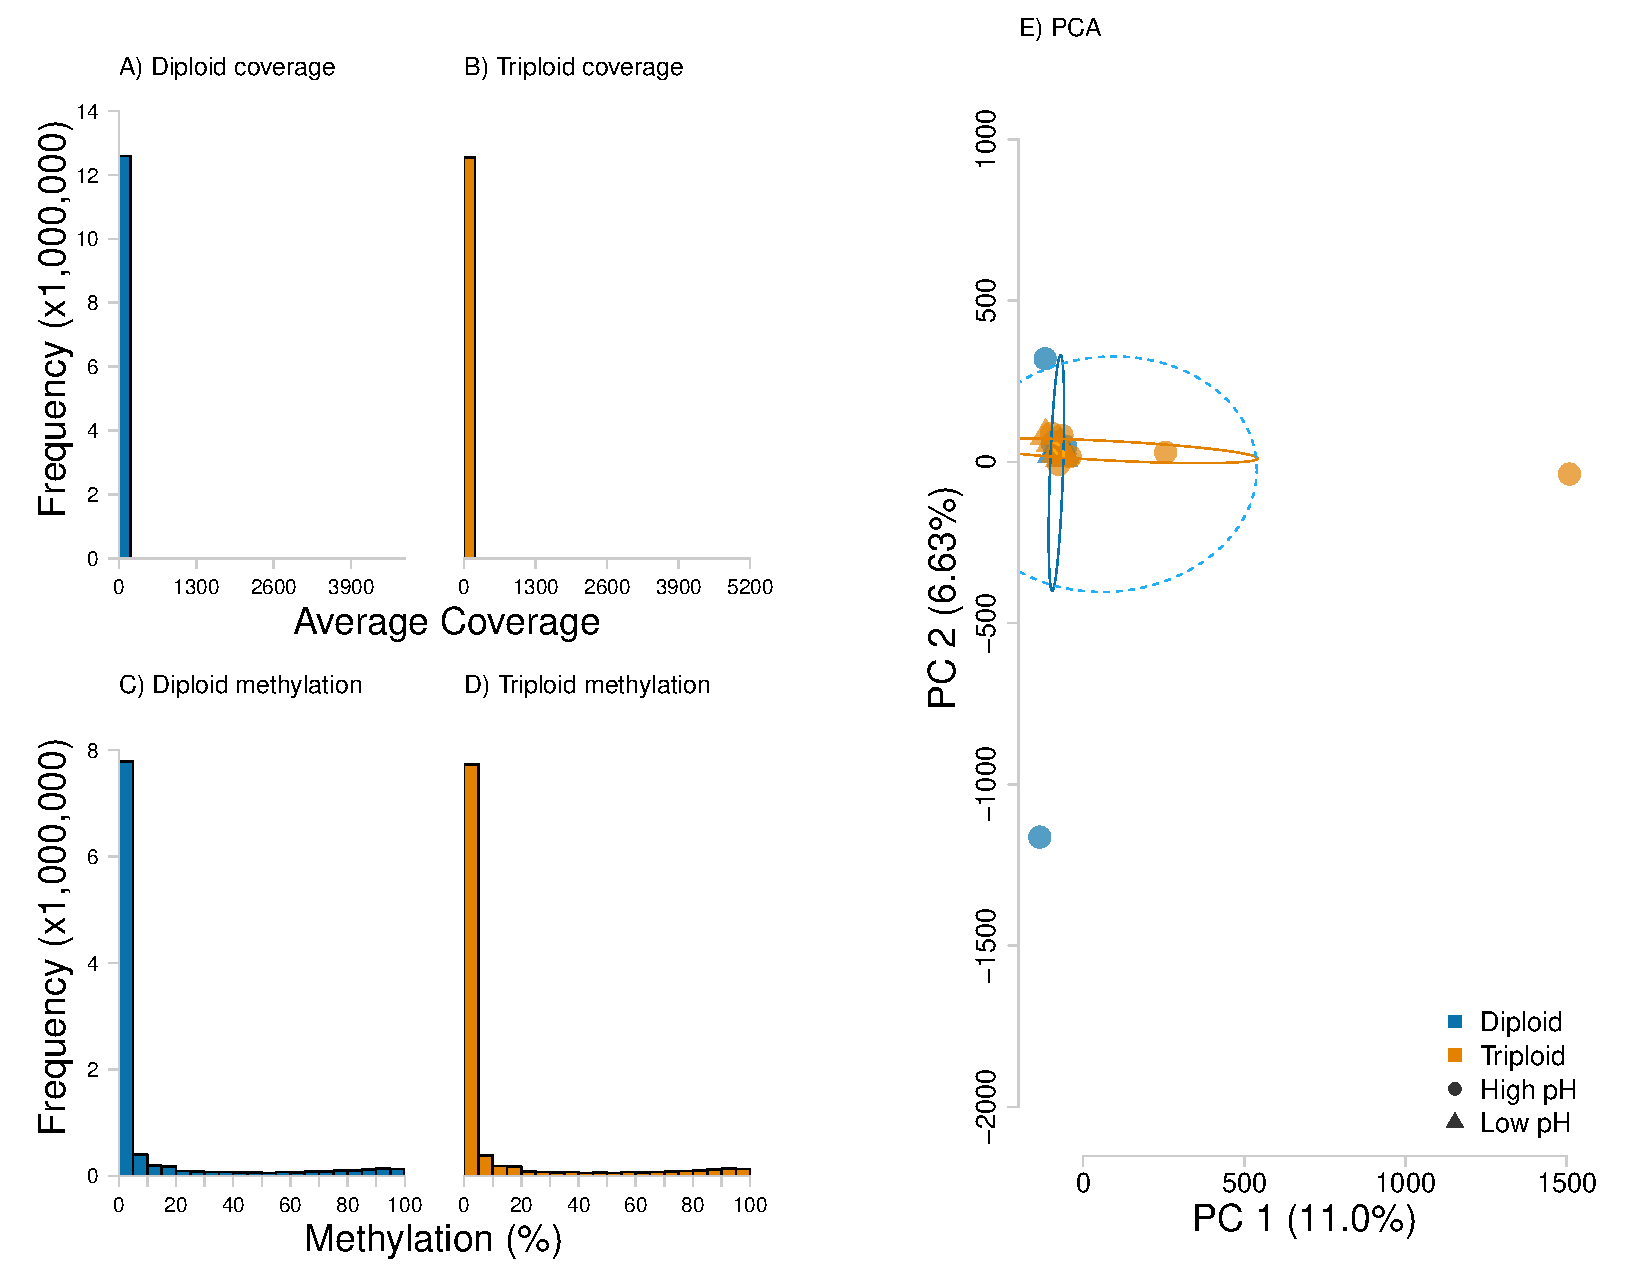
\includegraphics[width=1\textwidth]{figure/Ch4/Figure4.1.pdf}
  \caption{Diploid and triploid coverage and global methylation}
  \label{fig:coveragemeth}
\end{figure}
\clearpage

\textbf{Figure} \ref{fig:cpglocations}: Percent of total CpGs present in distinct \emph{C. gigas} genome features for various CpG categories (from left to right: all CpGs with at least 5x coverage in all samples, highly methylated CpGs, moderately methylated CpGs, and lowly methylated CpGs).\newline
\begin{figure}[h]
\centering
  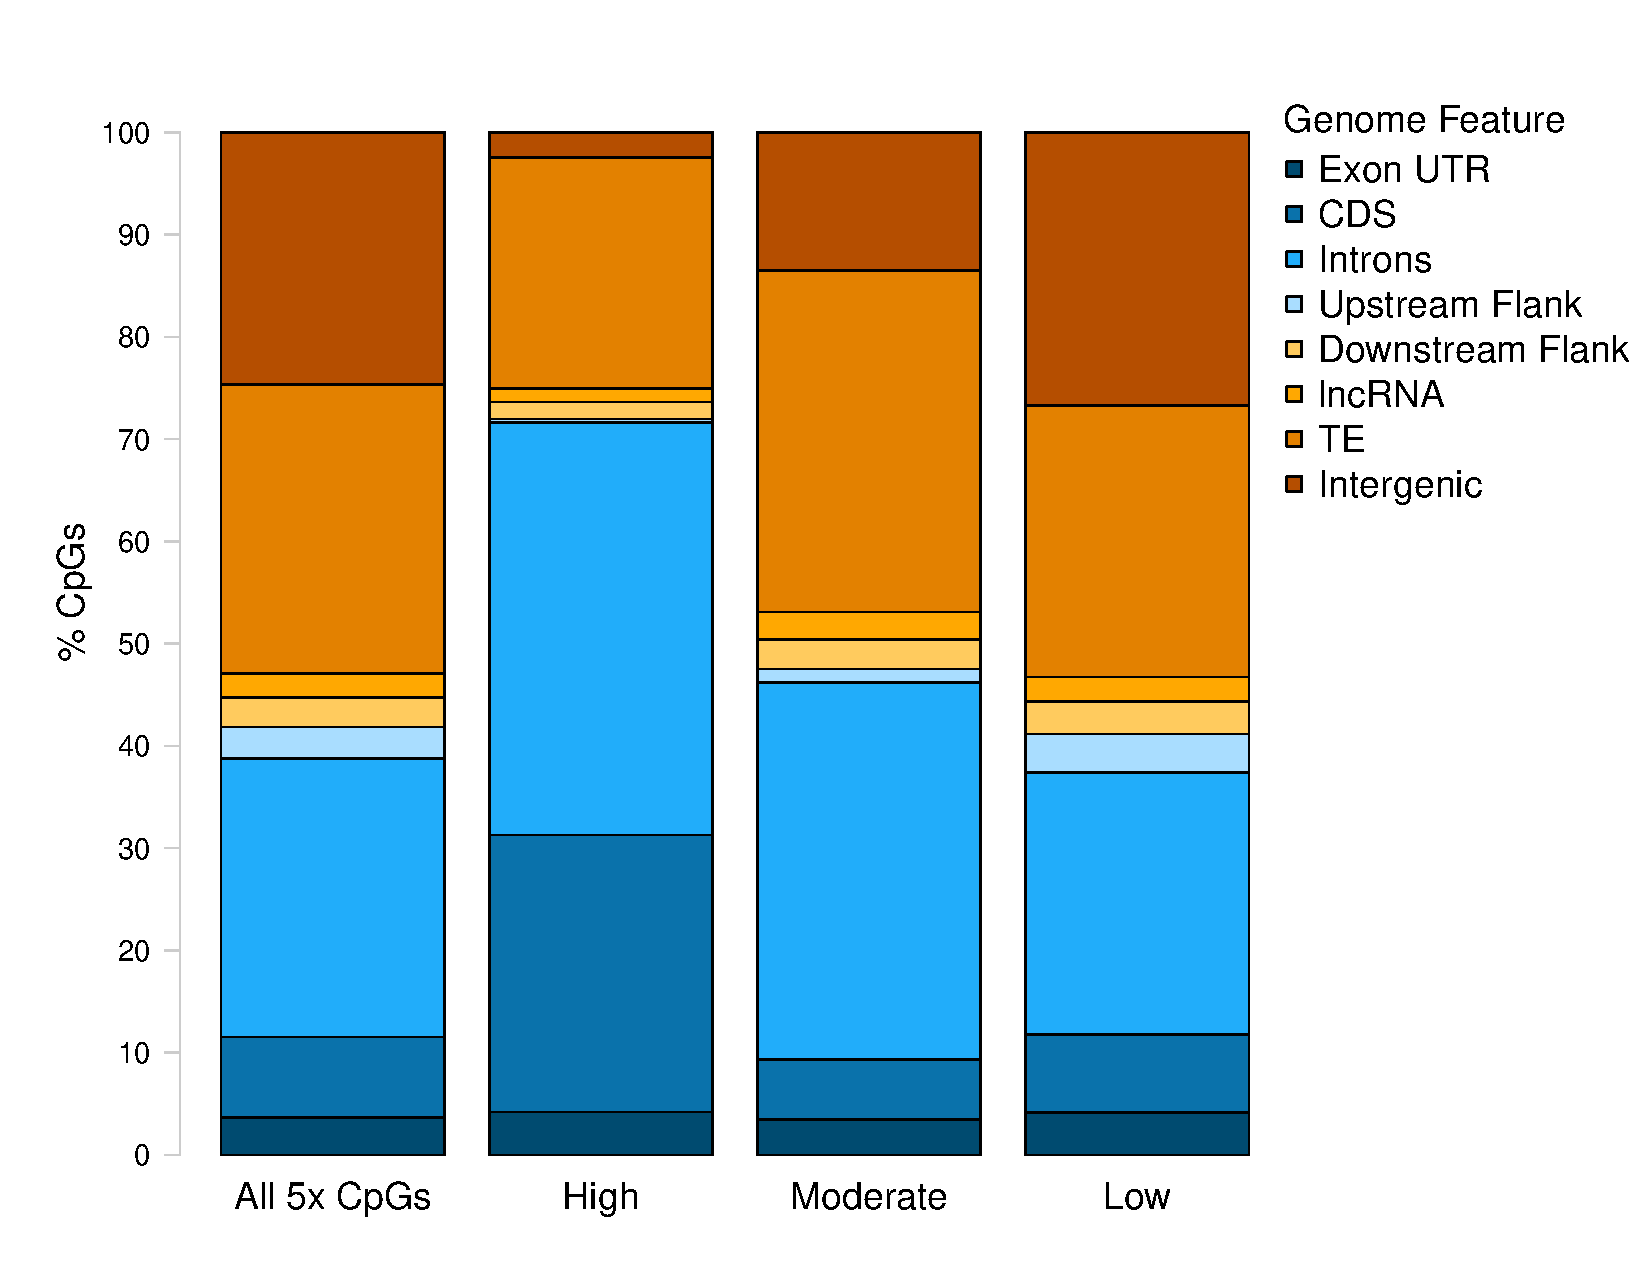
\includegraphics[width=1\textwidth]{figure/Ch4/Figure4.2.pdf}
  \caption{Genome distribution of various CpG categories}
  \label{fig:cpglocations}
\end{figure}
\clearpage

\textbf{Figure} \ref{fig:multiheatmap}: Heatmap of A) ploidy-, B) pH-, and C) interaction-DML identified, and D) distribution in \emph{C. gigas} chromosomes. Density plots associated with heatmaps quantify the number of DML in various methylation bins.\newline
\begin{figure}[h]
\centering
  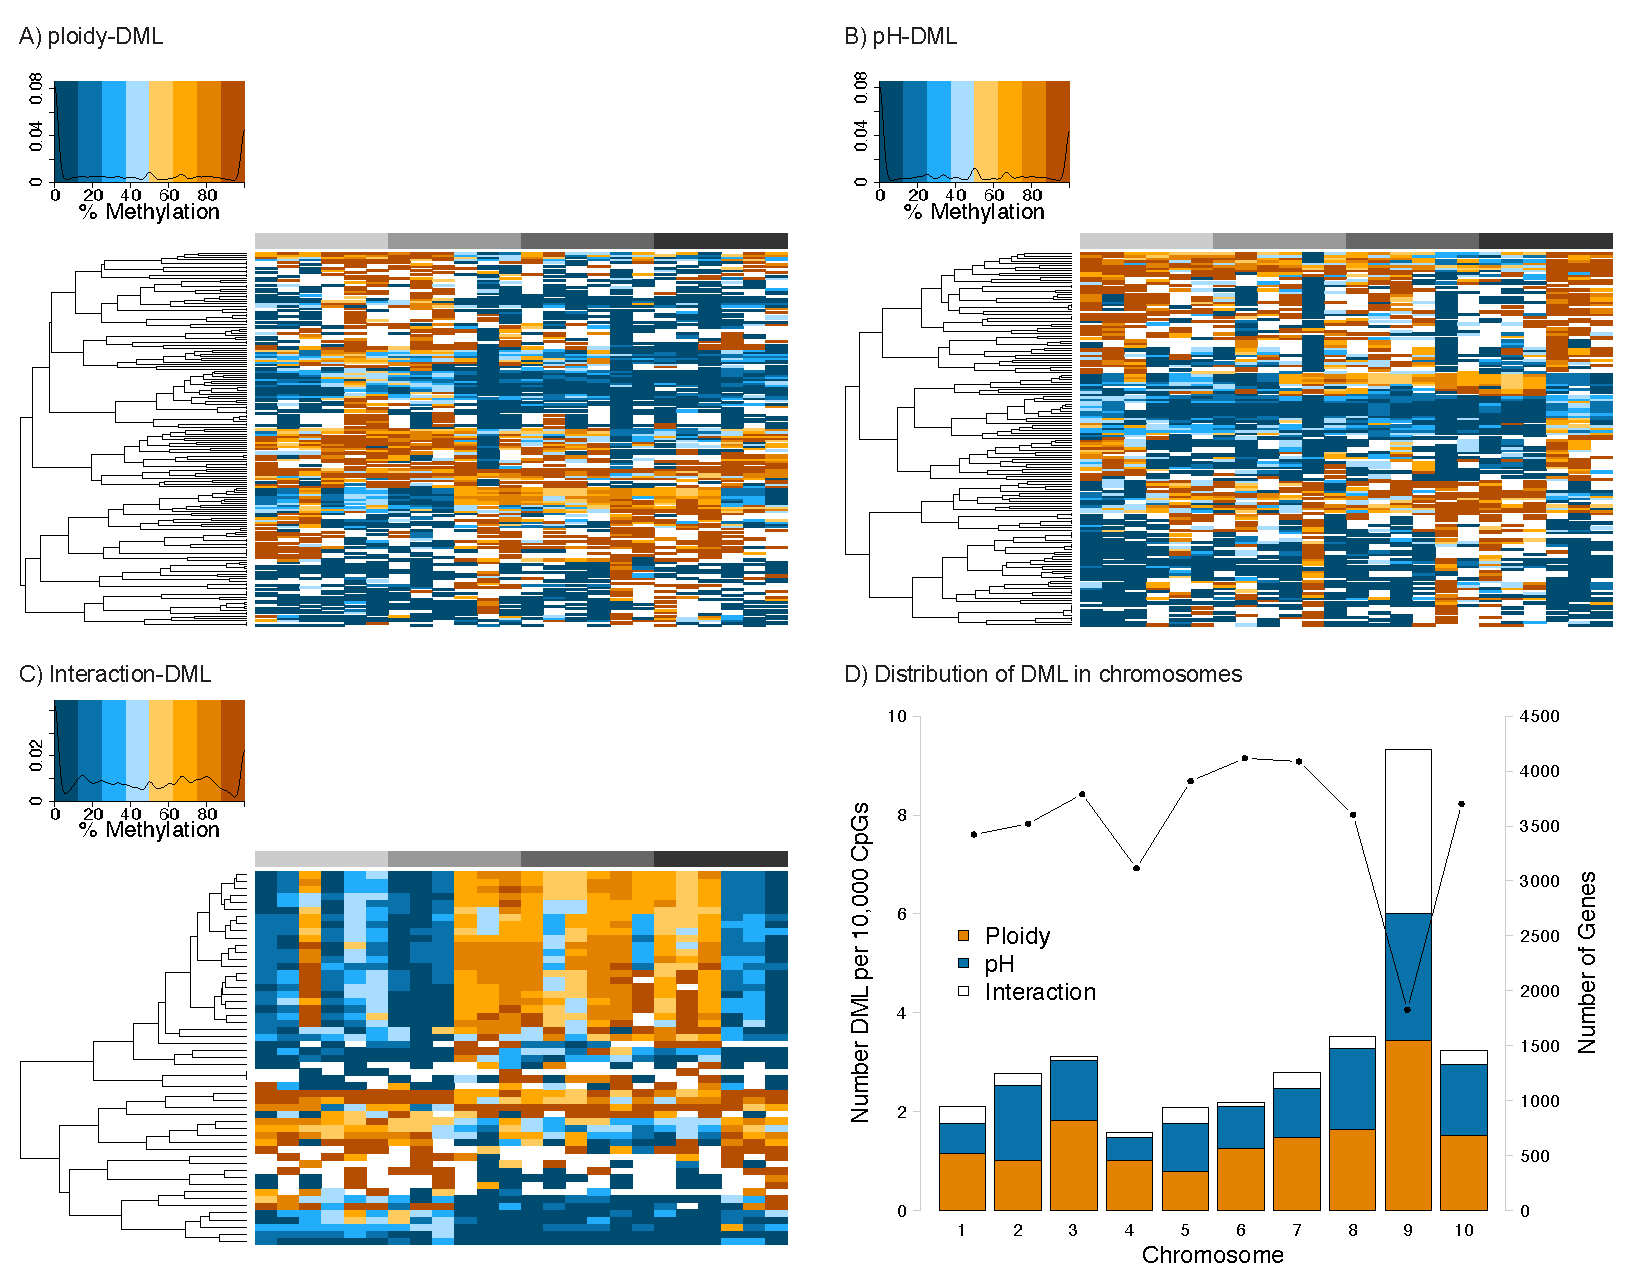
\includegraphics[width=1\textwidth]{figure/Ch4/Figure4.3.pdf}
  \caption{DML heatmaps and chromosomal distribution}
  \label{fig:multiheatmap}
\end{figure}
\clearpage

\textbf{Figure} \ref{fig:DMLgenomicloc}: Distribution of all 5x CpGs, ploidy-DML, pH-DML, and interaction-DML in various \emph{C. gigas} genome features.\newline
\begin{figure}[h]
\centering
  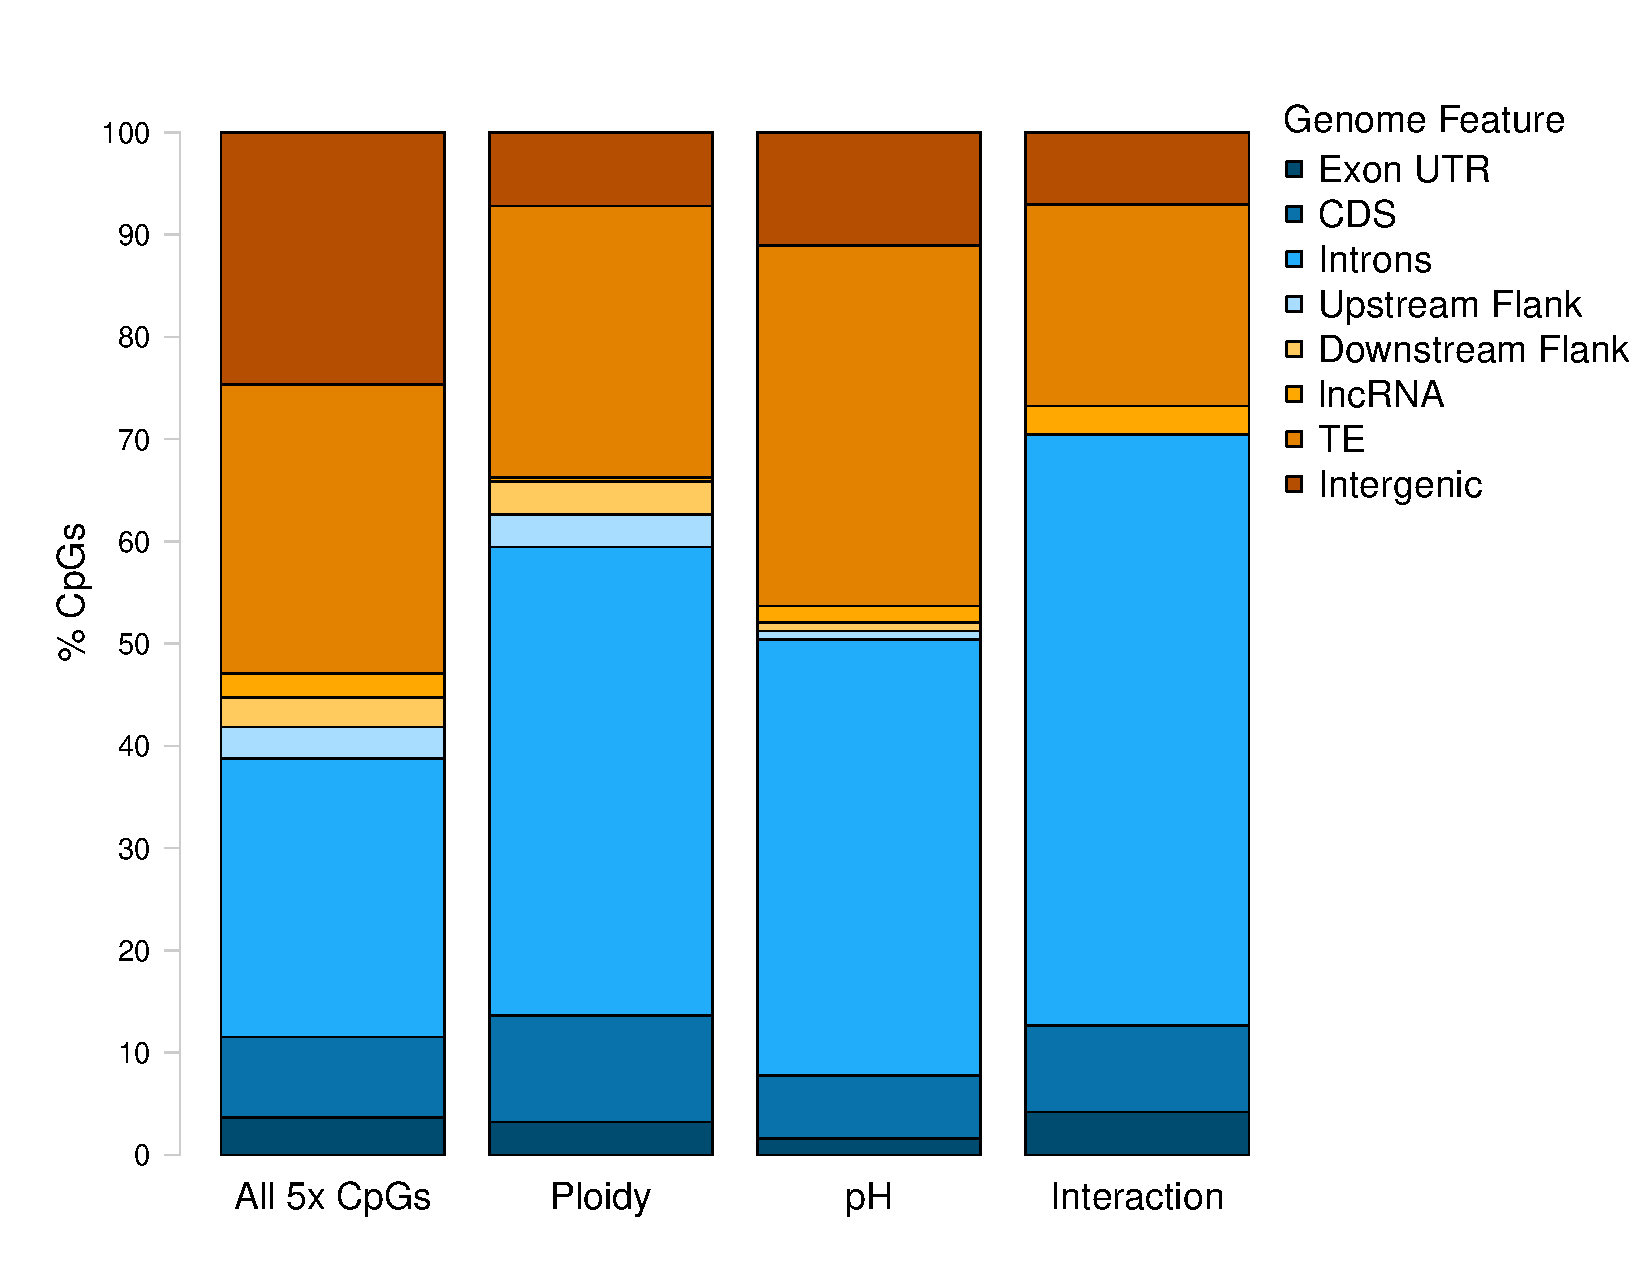
\includegraphics[width=1\textwidth]{figure/Ch4/Figure4.4.pdf}
  \caption{DML heatmaps and chromosomal distribution}
  \label{fig:DMLgenomicloc}
\end{figure}
\clearpage

\hypertarget{conclusion-4}{%
\chapter*{Conclusion}\label{conclusion-4}}
\addcontentsline{toc}{chapter}{Conclusion}

While extensive research has explored how ocean acidification can act as a selective force upon less tolerant phenotypes and associated genotypes from a population and allow resilient ones to proliferate (\protect\hyperlink{ref-Bitter2019}{Bitter, Kapsenberg, Gattuso, \& Pfister, 2019}; \protect\hyperlink{ref-Logan2021}{Logan, Dunne, Ryan, Baskett, \& Donner, 2021}; \protect\hyperlink{ref-Sunday2014}{Sunday et al., 2014}; \protect\hyperlink{ref-Sunday2011}{Sunday, Crim, Harley, \& Hart, 2011}), this framework may not account for sublethal or nonlethal impacts that are not easily documented. Without understanding these impacts, we are unable to connect observed phenotypes with physiological mechanisms defining environmental responses. My dissertation uses the Pacific oyster, \emph{Crassostrea gigas}, as a model organism to demonstrate how proteomic and epigenetic analysis can elucidate sub- and nonlethal impacts of ocean acidification on marine invertebrates. My findings can be used to expand the conceptual model used to interpret low pH impacts on physiology.

Importantly, my dissertation helps elucidate the functional role of environmentally-responsive DNA methylation. Concentration of methylation in genes suggests a role in regulating gene expression. Methylation may reduce transcriptional noise so C. gigas can be more efficient when maintaining homeostasis under stressful conditions (\protect\hyperlink{ref-Roberts2012}{Roberts \& Gavery, 2012}). My finding that somatic and reproductive have distinct responses to low pH stress is characteristic of these tissues having different roles within an organism. To maintain tissue function, different processes would need to be targeted via changes in gene methylation.

Methylation control of transcriptional processes could allow organisms to acclimate to ocean acidification, changing the outcome of selection. If the environment remains stable and offspring inherit these methylation patterns, then selection outcomes would again be altered. However, organisms may require spurious transcription if the environment is unpredictable or variable, such as temporary low pH events associated with seasonal upwelling. In this case, methylation regulation of transcription would not provide resilience and could lead to poorer survival. Even if less-tolerant genotypes are unable to deregulate transcriptional processes in a fluctuating environment, resource competition with tolerant genotypes while alive could impact fitness of those tolerant genotypes. Therefore, it is critical to consider methylation when considering the ramifications of ocean acidification not only at an organismal level, but at an ecological level. With my dissertation as a foundation, future work can explore the role of DNA methylation in modulating carryover effects to environmental stressors, and determine how methylation can interact with gene expression, protein abundance, or other epigenomic mechanisms to shape physiological phenotype and ecological interactions.

\appendix

\hypertarget{appendix-1}{%
\chapter{Appendix 1}\label{appendix-1}}

Data accessibility information and additional materials for each dissertation chapter can be found below.

\hypertarget{chapter-1-characterization-of-pacific-oyster-crassostrea-gigas-proteomic-response-to-natural-environmental-differences}{%
\section{\texorpdfstring{Chapter 1: Characterization of Pacific oyster (\emph{Crassostrea gigas}) proteomic response to natural environmental differences}{Chapter 1: Characterization of Pacific oyster (Crassostrea gigas) proteomic response to natural environmental differences}}\label{chapter-1-characterization-of-pacific-oyster-crassostrea-gigas-proteomic-response-to-natural-environmental-differences}}

Raw data can be accessed in the PeptideAtlas under accession PASS01304 and PASS01305. Skyline documents can be found on Panorama Public. All scripts and workflows can be found in the associated Github repository (\url{https://github.com/RobertsLab/paper-gigas-DNR-proteomics}), which is archived on Figshare (\url{https://doi.org/10.6084/m9.figshare.7450997.v2}).

\hypertarget{chapter-2-larval-response-to-parental-low-ph-exposure-in-pacific-oysters-crassostrea-gigas}{%
\section{\texorpdfstring{Chapter 2: Larval response to parental low pH exposure in Pacific oysters (\emph{Crassostrea gigas})}{Chapter 2: Larval response to parental low pH exposure in Pacific oysters (Crassostrea gigas)}}\label{chapter-2-larval-response-to-parental-low-ph-exposure-in-pacific-oysters-crassostrea-gigas}}

All scripts and workflows can be found in the associated Github repository (\url{https://github.com/RobertsLab/paper-gigas-early-gametogenic-exposure}), which is archived on Figshare (\url{https://doi.org/10.6084/m9.figshare.7155074.v2}).

Additional histology can be found in this repository, including microscope images (\url{https://github.com/RobertsLab/paper-gigas-early-gametogenic-exposure/tree/master/images/Gigas-gonad-histology}) and specific sex information for each individual sampled (\url{https://github.com/RobertsLab/paper-gigas-early-gametogenic-exposure/blob/master/data/2017-Adult-Gigas-Tissue-Sampling/2018-02-27-Gigas-Histology-Classification.csv}).

\hypertarget{chapter-3-low-ph-influences-methylation-patterns-of-gonad-growth-genes-in-the-pacific-oyster-crassostrea-gigas}{%
\section{\texorpdfstring{Chapter 3: Low pH influences methylation patterns of gonad growth genes in the Pacific oyster (\emph{Crassostrea gigas})}{Chapter 3: Low pH influences methylation patterns of gonad growth genes in the Pacific oyster (Crassostrea gigas)}}\label{chapter-3-low-ph-influences-methylation-patterns-of-gonad-growth-genes-in-the-pacific-oyster-crassostrea-gigas}}

All data, scripts, workflows, and outputs can be found in the associated Github repository (\url{https://github.com/RobertsLab/project-gigas-oa-meth}), including:
\begin{itemize}
\tightlist
\item
  A summary of sequencing and trimming information: \url{https://github.com/RobertsLab/project-gigas-oa-meth/blob/master/output/12-functional-enrichment/all-CC-EnrichedGO-DML-withTranscript.csv}
\item
  Chi-squared test output comparing genomic locations of highly methylated CpGs against all CpGs with 5x data: \url{https://github.com/RobertsLab/project-gigas-oa-meth/blob/master/output/09-methylation-landscape/CpG-location-statResults.txt}
\item
  Principal Components Analysis visualizing global methylation patterns: \url{https://github.com/RobertsLab/project-gigas-oa-meth/blob/master/output/06-methylKit/figures/all-sample-PCA.pdf}
\item
  Plot of pairwise Pearson's Correlations for global methylation: \url{https://github.com/RobertsLab/project-gigas-oa-meth/blob/master/output/06-methylKit/general-stats/Full-Sample-Pearson-Correlation-Plot-FilteredCov5Destrand.jpeg}
\item
  Chromosomal distribution of DML, including number of DML in scaffolds not placed in any chromosome: \url{https://github.com/RobertsLab/project-gigas-oa-meth/blob/master/output/06-methylKit/DML/All-DML-by-chr.csv}
\item
  Number of DML in genes: \url{https://github.com/RobertsLab/project-gigas-oa-meth/blob/master/output/10_DML-characterization/Number-of-DML-per-Gene.csv}
\item
  Chi-squared test output comparing genomic locations of DML against all CpGs with 5x data: \url{https://github.com/RobertsLab/project-gigas-oa-meth/blob/master/output/10_DML-characterization/CpG-location-statResults-All.txt}
\item
  \texttt{simplifyEnrichment} figure for enriched cellular components: \url{https://github.com/RobertsLab/project-gigas-oa-meth/blob/master/output/12-functional-enrichment/figures/simplifyEnrichment-CC.pdf}
\item
  Enriched biological process GO terms and associated gene and transcript information: \url{https://github.com/RobertsLab/project-gigas-oa-meth/blob/master/output/12-functional-enrichment/all-BP-EnrichedGO-DML-withTranscript.csv}
\item
  Enriched cellular component GO terms and associated gene and transcript information: \url{https://github.com/RobertsLab/project-gigas-oa-meth/blob/master/output/12-functional-enrichment/all-CC-EnrichedGO-DML-withTranscript.csv}
\end{itemize}
\hypertarget{chapter-4-polyploidy-and-environmental-stress-have-distinct-impacts-on-pacific-oyster-crassostrea-gigas-ctenidia-methylomes}{%
\section{\texorpdfstring{Chapter 4: Polyploidy and environmental stress have distinct impacts on Pacific oyster (\emph{Crassostrea gigas}) ctenidia methylomes}{Chapter 4: Polyploidy and environmental stress have distinct impacts on Pacific oyster (Crassostrea gigas) ctenidia methylomes}}\label{chapter-4-polyploidy-and-environmental-stress-have-distinct-impacts-on-pacific-oyster-crassostrea-gigas-ctenidia-methylomes}}

All data, scripts, workflows, and outputs can be found in the associated Github repository (\url{https://github.com/RobertsLab/project-oyster-oa}), including:
\begin{itemize}
\tightlist
\item
  Chi-squared test output comparing genomic locations of highly methylated CpGs against all CpGs with 5x data: \url{https://github.com/RobertsLab/project-oyster-oa/blob/master/analyses/Haws_06-methylation-landscape/CpG-location-statResults.txt}
\item
  Plot of pairwise Pearson's Correlations for global methylation: \url{https://github.com/RobertsLab/project-oyster-oa/blob/master/analyses/Haws_04-methylKit/general-stats/Full-Sample-Pearson-Correlation-Plot-FilteredCov5Destrand.jpeg}
\item
  Chromosomal distribution of ploidy-DML, including number of ploidy-DML in scaffolds not placed in any chromosome: \url{https://github.com/RobertsLab/project-oyster-oa/blob/master/analyses/Haws_04-DSS/DML/ploidy-DML-by-chr.csv}
\item
  Chromosomal distribution of pH-DML, including number of pH-DML in scaffolds not placed in any chromosome: \url{https://github.com/RobertsLab/project-oyster-oa/blob/master/analyses/Haws_04-DSS/DML/pH-DML-by-chr.csv}
\item
  Chromosomal distribution of interaction-DML, including number of interaction-DML in scaffolds not placed in any chromosome: \url{https://github.com/RobertsLab/project-oyster-oa/blob/master/analyses/Haws_04-DSS/DML/ploidypH-DML-by-chr.csv}
\item
  Number of ploidy-DML in genes: \url{https://github.com/RobertsLab/project-oyster-oa/blob/master/analyses/Haws_07-DML-characterization/Number-of-ploidy-DML-per-Gene.csv}
\item
  Number of pH-DML in genes: \url{https://github.com/RobertsLab/project-oyster-oa/blob/master/analyses/Haws_07-DML-characterization/Number-of-pH-DML-per-Gene.csv}
\item
  Number of interaction-DML in genes: \url{https://github.com/RobertsLab/project-oyster-oa/blob/master/analyses/Haws_07-DML-characterization/Number-of-ploidypH-DML-per-Gene.csv}
\item
  Chi-squared test output comparing genomic locations of ploidy-DML against all CpGs with 5x data: \url{https://github.com/RobertsLab/project-oyster-oa/blob/master/analyses/Haws_07-DML-characterization/CpG-location-statResults-ploidy.txt}
\item
  Chi-squared test output comparing genomic locations of pH-DML against all CpGs with 5x data: \url{https://github.com/RobertsLab/project-oyster-oa/blob/master/analyses/Haws_07-DML-characterization/CpG-location-statResults-pH.txt}
\item
  Chi-squared test output comparing genomic locations of interaction-DML against all CpGs with 5x data: \url{https://github.com/RobertsLab/project-oyster-oa/blob/master/analyses/Haws_07-DML-characterization/CpG-location-statResults-ploidypH.txt}
\item
  \texttt{simplifyEnrichment} figure for enriched biological process terms associated with ploidy-DML: \url{https://github.com/RobertsLab/project-oyster-oa/blob/master/analyses/Haws_09-functional-enrichment/figures/simplifyEnrichment-ploidy-BP.pdf}
\item
  Enriched biological process GO terms and associated gene and transcript information for ploidy-DML: \url{https://github.com/RobertsLab/project-oyster-oa/blob/master/analyses/Haws_09-functional-enrichment/ploidy-BP-FisherTestResults.csv}
\item
  \texttt{simplifyEnrichment} figure for enriched biological process terms associated with pH-DML: \url{https://github.com/RobertsLab/project-oyster-oa/blob/master/analyses/Haws_09-functional-enrichment/figures/simplifyEnrichment-pH-BP.pdf}
\item
  Enriched biological process GO terms and associated gene and transcript information for pH-DML: \url{https://github.com/RobertsLab/project-oyster-oa/blob/master/analyses/Haws_09-functional-enrichment/pH-BP-FisherTestResults.csv}
\item
  \texttt{simplifyEnrichment} figure for enriched molecular function terms associated with pH-DML: \url{https://github.com/RobertsLab/project-oyster-oa/blob/master/analyses/Haws_09-functional-enrichment/figures/simplifyEnrichment-pH-MF.pdf}
\item
  Enriched molecular function GO terms and associated gene and transcript information for pH-DML: \url{https://github.com/RobertsLab/project-oyster-oa/blob/master/analyses/Haws_09-functional-enrichment/pH-MF-FisherTestResults.csv}
\end{itemize}
\hypertarget{colophon}{%
\chapter*{Colophon}\label{colophon}}
\addcontentsline{toc}{chapter}{Colophon}

This document is set in \href{https://github.com/georgd/EB-Garamond}{EB Garamond}, \href{https://github.com/adobe-fonts/source-code-pro/}{Source Code Pro} and \href{http://www.latofonts.com/lato-free-fonts/}{Lato}. The body text is set at 11pt with \(\familydefault\).

It was written in R Markdown and \(\LaTeX\), and rendered into PDF using \href{https://github.com/benmarwick/huskydown}{huskydown} and \href{https://github.com/rstudio/bookdown}{bookdown}.

This document was typeset using the XeTeX typesetting system, and the \href{http://staff.washington.edu/fox/tex/}{University of Washington Thesis class} class created by Jim Fox. Under the hood, the \href{https://github.com/UWIT-IAM/UWThesis}{University of Washington Thesis LaTeX template} is used to ensure that documents conform precisely to submission standards. Other elements of the document formatting source code have been taken from the \href{https://github.com/stevenpollack/ucbthesis}{Latex, Knitr, and RMarkdown templates for UC Berkeley's graduate thesis}, and \href{https://github.com/suchow/Dissertate}{Dissertate: a LaTeX dissertation template to support the production and typesetting of a PhD dissertation at Harvard, Princeton, and NYU}

The source files for this thesis, along with all the data files, have been organised into an R package, xxx, which is available at \url{https://github.com/xxx/xxx}. A hard copy of the thesis can be found in the University of Washington library.

This version of the thesis was generated on 2021-08-20 15:41:53. The repository is currently at this commit:

The computational environment that was used to generate this version is as follows:
\begin{verbatim}
- Session info ---------------------------------------------------------------
 setting  value                       
 version  R version 4.1.0 (2021-05-18)
 os       macOS Big Sur 10.16         
 system   x86_64, darwin17.0          
 ui       X11                         
 language (EN)                        
 collate  en_US.UTF-8                 
 ctype    en_US.UTF-8                 
 tz       America/Los_Angeles         
 date     2021-08-20                  

- Packages -------------------------------------------------------------------
 package     * version date       lib source                               
 assertthat    0.2.1   2019-03-21 [1] CRAN (R 4.1.0)                       
 bookdown      0.23.1  2021-08-18 [1] Github (rstudio/bookdown@6643bb9)    
 cachem        1.0.5   2021-05-15 [1] CRAN (R 4.1.0)                       
 callr         3.7.0   2021-04-20 [1] CRAN (R 4.1.0)                       
 cli           3.0.1   2021-07-17 [1] CRAN (R 4.1.0)                       
 colorspace    2.0-2   2021-06-24 [1] CRAN (R 4.1.0)                       
 crayon        1.4.1   2021-02-08 [1] CRAN (R 4.1.0)                       
 DBI           1.1.1   2021-01-15 [1] CRAN (R 4.1.0)                       
 desc          1.3.0   2021-03-05 [1] CRAN (R 4.1.0)                       
 devtools    * 2.4.2   2021-06-07 [1] CRAN (R 4.1.0)                       
 digest        0.6.27  2020-10-24 [1] CRAN (R 4.1.0)                       
 dplyr       * 1.0.7   2021-06-18 [1] CRAN (R 4.1.0)                       
 ellipsis      0.3.2   2021-04-29 [1] CRAN (R 4.1.0)                       
 evaluate      0.14    2019-05-28 [1] CRAN (R 4.1.0)                       
 fansi         0.5.0   2021-05-25 [1] CRAN (R 4.1.0)                       
 fastmap       1.1.0   2021-01-25 [1] CRAN (R 4.1.0)                       
 fs            1.5.0   2020-07-31 [1] CRAN (R 4.1.0)                       
 generics      0.1.0   2020-10-31 [1] CRAN (R 4.1.0)                       
 ggplot2       3.3.5   2021-06-25 [1] CRAN (R 4.1.0)                       
 git2r         0.28.0  2021-01-10 [1] CRAN (R 4.1.0)                       
 glue          1.4.2   2020-08-27 [1] CRAN (R 4.1.0)                       
 gtable        0.3.0   2019-03-25 [1] CRAN (R 4.1.0)                       
 htmltools     0.5.1.1 2021-01-22 [1] CRAN (R 4.1.0)                       
 httr          1.4.2   2020-07-20 [1] CRAN (R 4.1.0)                       
 huskydown   * 0.0.5   2021-08-18 [1] Github (benmarwick/huskydown@addb48e)
 kableExtra    1.3.4   2021-02-20 [1] CRAN (R 4.1.0)                       
 knitr         1.33    2021-04-24 [1] CRAN (R 4.1.0)                       
 lifecycle     1.0.0   2021-02-15 [1] CRAN (R 4.1.0)                       
 magrittr      2.0.1   2020-11-17 [1] CRAN (R 4.1.0)                       
 memoise       2.0.0   2021-01-26 [1] CRAN (R 4.1.0)                       
 munsell       0.5.0   2018-06-12 [1] CRAN (R 4.1.0)                       
 pillar        1.6.2   2021-07-29 [1] CRAN (R 4.1.0)                       
 pkgbuild      1.2.0   2020-12-15 [1] CRAN (R 4.1.0)                       
 pkgconfig     2.0.3   2019-09-22 [1] CRAN (R 4.1.0)                       
 pkgload       1.2.1   2021-04-06 [1] CRAN (R 4.1.0)                       
 prettyunits   1.1.1   2020-01-24 [1] CRAN (R 4.1.0)                       
 processx      3.5.2   2021-04-30 [1] CRAN (R 4.1.0)                       
 ps            1.6.0   2021-02-28 [1] CRAN (R 4.1.0)                       
 purrr         0.3.4   2020-04-17 [1] CRAN (R 4.1.0)                       
 R6            2.5.0   2020-10-28 [1] CRAN (R 4.1.0)                       
 remotes       2.4.0   2021-06-02 [1] CRAN (R 4.1.0)                       
 rlang         0.4.11  2021-04-30 [1] CRAN (R 4.1.0)                       
 rmarkdown     2.10    2021-08-06 [1] CRAN (R 4.1.0)                       
 rprojroot     2.0.2   2020-11-15 [1] CRAN (R 4.1.0)                       
 rstudioapi    0.13    2020-11-12 [1] CRAN (R 4.1.0)                       
 rvest         1.0.0   2021-03-09 [1] CRAN (R 4.1.0)                       
 scales        1.1.1   2020-05-11 [1] CRAN (R 4.1.0)                       
 sessioninfo   1.1.1   2018-11-05 [1] CRAN (R 4.1.0)                       
 stringi       1.7.3   2021-07-16 [1] CRAN (R 4.1.0)                       
 stringr       1.4.0   2019-02-10 [1] CRAN (R 4.1.0)                       
 svglite       2.0.0   2021-02-20 [1] CRAN (R 4.1.0)                       
 systemfonts   1.0.2   2021-05-11 [1] CRAN (R 4.1.0)                       
 testthat      3.0.4   2021-07-01 [1] CRAN (R 4.1.0)                       
 tibble        3.1.3   2021-07-23 [1] CRAN (R 4.1.0)                       
 tidyselect    1.1.1   2021-04-30 [1] CRAN (R 4.1.0)                       
 usethis     * 2.0.1   2021-02-10 [1] CRAN (R 4.1.0)                       
 utf8          1.2.2   2021-07-24 [1] CRAN (R 4.1.0)                       
 vctrs         0.3.8   2021-04-29 [1] CRAN (R 4.1.0)                       
 viridisLite   0.4.0   2021-04-13 [1] CRAN (R 4.1.0)                       
 webshot       0.5.2   2019-11-22 [1] CRAN (R 4.1.0)                       
 withr         2.4.2   2021-04-18 [1] CRAN (R 4.1.0)                       
 xfun          0.25    2021-08-06 [1] CRAN (R 4.1.0)                       
 xml2          1.3.2   2020-04-23 [1] CRAN (R 4.1.0)                       
 yaml          2.2.1   2020-02-01 [1] CRAN (R 4.1.0)                       

[1] /Library/Frameworks/R.framework/Versions/4.1/Resources/library
\end{verbatim}
\backmatter

\hypertarget{references}{%
\chapter*{References}\label{references}}
\addcontentsline{toc}{chapter}{References}

\markboth{References}{References}

\noindent

\setlength{\parindent}{-0.20in}
\setlength{\leftskip}{0.20in}
\setlength{\parskip}{8pt}

\hypertarget{refs}{}
\begin{CSLReferences}{1}{0}
\leavevmode\hypertarget{ref-Abele2007}{}%
Abele, E., Philip, E., Gonzalez, P. M., \& Puntarulo, S. (2007). {Marine invertebrate mitochondria and oxidative stress}. \emph{Front. Biosci.}, \emph{12}, 933--946.

\leavevmode\hypertarget{ref-Adams2005}{}%
Adams, K. L., \& Wendel, J. F. (2005). {Polyploidy and genome evolution in plants}. \emph{Curr. Opin. Plant Biol.}, \emph{8}(2), 135--141. http://doi.org/\href{https://doi.org/10.1016/j.pbi.2005.01.001}{10.1016/j.pbi.2005.01.001}

\leavevmode\hypertarget{ref-Akalin2012}{}%
Akalin, A., Kormaksson, M., Li, S., Garrett-Bakelman, F. E., Figueroa, M. E., Melnick, A., \& Mason, C. E. (2012). {methylKit: a comprehensive R package for the analysis of genome-wide DNA methylation profiles}. \emph{Genome Biol.}, \emph{13}(10), R87. http://doi.org/\href{https://doi.org/10.1186/gb-2012-13-10-r87}{10.1186/gb-2012-13-10-r87}

\leavevmode\hypertarget{ref-Alexa2010}{}%
Alexa, A., Rahnenfuhrer, J., \& Others. (2010). {topGO: enrichment analysis for gene ontology}. \emph{R Package Version}, \emph{2}(0), 2010.

\leavevmode\hypertarget{ref-Allen2008}{}%
Allen, R. M., Buckley, Y. M., \& Marshall, D. J. (2008). {Offspring size plasticity in response to intraspecific competition: an adaptive maternal effect across life-history stages}. \emph{Am. Nat.}, \emph{171}(2), 225--237. http://doi.org/\href{https://doi.org/10.1086/524952}{10.1086/524952}

\leavevmode\hypertarget{ref-Andrews2010}{}%
Andrews, S. (2010). {FastQC: a quality control tool for high throughput sequence data}. Babraham Bioinformatics, Babraham Institute, Cambridge, United Kingdom.

\leavevmode\hypertarget{ref-Arredondo-Espinoza2021}{}%
Arredondo-Espinoza, R., Ibarra, A. M., Roberts, S. B., Sicard-Gonzalez, M. T., \& Escobedo-Fregoso, C. (2021). {Differentially methylated gene regions between resistant and susceptible heat-phenotypes of the Pacific oyster \emph{Crassostrea gigas}}. \emph{Aquaculture}, \emph{543}, 736923. http://doi.org/\href{https://doi.org/10.1016/j.aquaculture.2021.736923}{10.1016/j.aquaculture.2021.736923}

\leavevmode\hypertarget{ref-Banas2004}{}%
Banas, N. S., Hickey, B. M., MacCready, P., \& Newton, J. A. (2004). {Dynamics of Willapa Bay, Washington: A Highly Unsteady, Partially Mixed Estuary}. \emph{J. Phys. Oceanogr.}, \emph{34}(11), 2413--2427. http://doi.org/\href{https://doi.org/10.1175/JPO2637.1}{10.1175/JPO2637.1}

\leavevmode\hypertarget{ref-Banas2007}{}%
Banas, N. S., Hickey, B. M., Newton, J. A., \& Ruesink, J. L. (2007). {Tidal exchange, bivalve grazing, and patterns of primary production in Willapa Bay, Washington, USA}. \emph{Mar. Ecol. Prog. Ser.}, \emph{341}, 123--139.

\leavevmode\hypertarget{ref-Bandstra2006}{}%
Bandstra, L., Hales, B., \& Takahashi, T. (2006). {High-frequency measurements of total {CO\(_2\)}: Method development and first oceanographic observations}. \emph{Mar. Chem.}, \emph{100}(1), 24--38. http://doi.org/\href{https://doi.org/10.1016/j.marchem.2005.10.009}{10.1016/j.marchem.2005.10.009}

\leavevmode\hypertarget{ref-Barros2013}{}%
Barros, P., Sobral, P., Range, P., Chı́charo, L., \& Matias, D. (2013). {Effects of sea-water acidification on fertilization and larval development of the oyster \emph{Crassostrea gigas}}. \emph{J. Exp. Mar. Bio. Ecol.}, \emph{440}, 200--206. http://doi.org/\href{https://doi.org/10.1016/j.jembe.2012.12.014}{10.1016/j.jembe.2012.12.014}

\leavevmode\hypertarget{ref-Barton2012}{}%
Barton, A., Hales, B., Waldbusser, G. G., Langdon, C., \& Feely, R. A. (2012). {The Pacific oyster, \emph{Crassostrea gigas} , shows negative correlation to naturally elevated carbon dioxide levels: Implications for near-term ocean acidification effects}. \emph{Limnol. Oceanogr.}, \emph{57}(3), 698--710. http://doi.org/\href{https://doi.org/10.4319/lo.2012.57.3.0698}{10.4319/lo.2012.57.3.0698}

\leavevmode\hypertarget{ref-Beyer2017}{}%
Beyer, J., Green, N. W., Brooks, S., Allan, I. J., Ruus, A., Gomes, T., \ldots{} Schøyen, M. (2017). {Blue mussels (\emph{Mytilus edulis spp}.) as sentinel organisms in coastal pollution monitoring: A review}. \emph{Mar. Environ. Res.}, \emph{130}, 338--365. http://doi.org/\href{https://doi.org/10.1016/j.marenvres.2017.07.024}{10.1016/j.marenvres.2017.07.024}

\leavevmode\hypertarget{ref-Bianucci2018}{}%
Bianucci, L., Long, W., Khangaonkar, T., Pelletier, G., Ahmed, A., Mohamedali, T., \ldots{} Figueroa-Kaminsky, C. (2018). {Sensitivity of the regional ocean acidification and carbonate system in Puget Sound to ocean and freshwater inputs}. \emph{Elem Sci Anth}, \emph{6}(1), 22. http://doi.org/\href{https://doi.org/10.1525/elementa.151}{10.1525/elementa.151}

\leavevmode\hypertarget{ref-Bible2017}{}%
Bible, J. M., Cheng, B. S., Chang, A. L., Ferner, M. C., Wasson, K., Zabin, C. J., \ldots{} Grosholz, E. D. (2017). {Timing of stressors alters interactive effects on a coastal foundation species}. \emph{Ecology}, \emph{98}(9), 2468--2478. http://doi.org/\href{https://doi.org/10.1002/ecy.1943}{10.1002/ecy.1943}

\leavevmode\hypertarget{ref-Bird2002}{}%
Bird, A. (2002). {DNA methylation patterns and epigenetic memory}. \emph{Genes Dev.}, \emph{16}(1), 6--21. http://doi.org/\href{https://doi.org/10.1101/gad.947102}{10.1101/gad.947102}

\leavevmode\hypertarget{ref-Bitter2019}{}%
Bitter, M. C., Kapsenberg, L., Gattuso, J.-P., \& Pfister, C. A. (2019). {Standing genetic variation fuels rapid adaptation to ocean acidification}. \emph{Nat. Commun.}, \emph{10}(1), 5821. http://doi.org/\href{https://doi.org/10.1038/s41467-019-13767-1}{10.1038/s41467-019-13767-1}

\leavevmode\hypertarget{ref-Bodenstein2021}{}%
Bodenstein, S., Walton, W. C., \& Steury, T. D. (2021). {Effect of farming practices on growth and mortality rates in triploid and diploid eastern oysters \emph{Crassostrea virginica}}. \emph{Aquac. Environ. Interact.}, \emph{13}, 33--40. http://doi.org/\href{https://doi.org/10.3354/aei00387}{10.3354/aei00387}

\leavevmode\hypertarget{ref-Bogan2020}{}%
Bogan, S. N., Johnson, K. M., \& Hofmann, G. E. (2020). {Changes in Genome-Wide Methylation and Gene Expression in Response to Future {pCO\(_2\)} Extremes in the Antarctic Pteropod \emph{Limacina helicina antarctica}}. \emph{Frontiers in Marine Science}, \emph{6}, 788. http://doi.org/\href{https://doi.org/10.3389/fmars.2019.00788}{10.3389/fmars.2019.00788}

\leavevmode\hypertarget{ref-Borges2018}{}%
Borges, F. O., Figueiredo, C., Sampaio, E., Rosa, R., \& Grilo, T. F. (2018). {Transgenerational deleterious effects of ocean acidification on the reproductive success of a keystone crustacean (\emph{Gammarus locusta})}. \emph{Mar. Environ. Res.}, \emph{138}, 55--64. http://doi.org/\href{https://doi.org/10.1016/j.marenvres.2018.04.006}{10.1016/j.marenvres.2018.04.006}

\leavevmode\hypertarget{ref-Boulais2017}{}%
Boulais, M., Chenevert, K. J., Demey, A. T., Darrow, E. S., Robison, M. R., Roberts, J. P., \& Volety, A. (2017). {Oyster reproduction is compromised by acidification experienced seasonally in coastal regions}. \emph{Sci. Rep.}, \emph{7}(1), 13276. http://doi.org/\href{https://doi.org/10.1038/s41598-017-13480-3}{10.1038/s41598-017-13480-3}

\leavevmode\hypertarget{ref-Boulais2018}{}%
Boulais, M., Suquet, M., Arsenault-Pernet, E. J., Malo, F., Queau, I., Pignet, P., \ldots{} Cosson, J. (2018). {pH controls spermatozoa motility in the Pacific oyster (\emph{Crassostrea gigas})}. \emph{Biol. Open}, \emph{7}(3). http://doi.org/\href{https://doi.org/10.1242/bio.031427}{10.1242/bio.031427}

\leavevmode\hypertarget{ref-Callam2016}{}%
Callam, B. R., Allen, S. K., \& Frank-Lawale, A. (2016). {Genetic and environmental influence on triploid \emph{Crassostrea virginica} grown in Chesapeake Bay: Growth}. \emph{Aquaculture}, \emph{452}, 97--106. http://doi.org/\href{https://doi.org/10.1016/j.aquaculture.2015.10.027}{10.1016/j.aquaculture.2015.10.027}

\leavevmode\hypertarget{ref-Campos2016}{}%
Campos, A., Danielsson, G., Farinha, A. P., Kuruvilla, J., Warholm, P., \& Cristobal, S. (2016). {Shotgun proteomics to unravel marine mussel (\emph{Mytilus edulis}) response to long-term exposure to low salinity and propranolol in a Baltic Sea microcosm}. \emph{J. Proteomics}, \emph{137}, 97--106. http://doi.org/\href{https://doi.org/10.1016/j.jprot.2016.01.010}{10.1016/j.jprot.2016.01.010}

\leavevmode\hypertarget{ref-Chambers2012}{}%
Chambers, M. C., Maclean, B., Burke, R., Amodei, D., Ruderman, D. L., Neumann, S., \ldots{} Mallick, P. (2012). {A cross-platform toolkit for mass spectrometry and proteomics}. \emph{Nat. Biotechnol.}, \emph{30}(10), 918--920. http://doi.org/\href{https://doi.org/10.1038/nbt.2377}{10.1038/nbt.2377}

\leavevmode\hypertarget{ref-ChandraRajan2021}{}%
Chandra Rajan, K., Yuan, M., Yu, Z., Roberts, S. B., \& Thiyagarajan, V. (2021). {Oyster biomineralisation under ocean acidification: from genes to shell}. \emph{Glob. Chang. Biol.} http://doi.org/\href{https://doi.org/10.1111/gcb.15675}{10.1111/gcb.15675}

\leavevmode\hypertarget{ref-Chapman2011}{}%
Chapman, R. W., Mancia, A., Beal, M., Veloso, A., Rathburn, C., Blair, A., \ldots{} Sanger, D. (2011). {The transcriptomic responses of the eastern oyster, \emph{Crassostrea virginica}, to environmental conditions}. \emph{Mol. Ecol.}, \emph{20}(7), 1431--1449. http://doi.org/\href{https://doi.org/10.1111/j.1365-294X.2011.05018.x}{10.1111/j.1365-294X.2011.05018.x}

\leavevmode\hypertarget{ref-Chen2006}{}%
Chen, Z. J., \& Ni, Z. (2006). {Mechanisms of genomic rearrangements and gene expression changes in plant polyploids}. \emph{Bioessays}, \emph{28}(3), 240--252. http://doi.org/\href{https://doi.org/10.1002/bies.20374}{10.1002/bies.20374}

\leavevmode\hypertarget{ref-Cornwall2016}{}%
Cornwall, C. E., \& Hurd, C. L. (2016). {Experimental design in ocean acidification research: problems and solutions}. \emph{ICES J. Mar. Sci.}, \emph{73}(3), 572--581. http://doi.org/\href{https://doi.org/10.1093/icesjms/fsv118}{10.1093/icesjms/fsv118}

\leavevmode\hypertarget{ref-Covelo-Soto2015}{}%
Covelo-Soto, L., Leunda, P. M., Pérez-Figueroa, A., \& Morán, P. (2015). {Genome-wide methylation study of diploid and triploid brown trout (\emph{Salmo trutta} L.)}. \emph{Anim. Genet.}, \emph{46}(3), 280--288. http://doi.org/\href{https://doi.org/10.1111/age.12287}{10.1111/age.12287}

\leavevmode\hypertarget{ref-DeDecker2011}{}%
De Decker, S., Normand, J., Saulnier, D., Pernet, F., Castagnet, S., \& Boudry, P. (2011). {Responses of diploid and triploid Pacific oysters \emph{Crassostrea gigas} to \emph{Vibrio} infection in relation to their reproductive status}. \emph{J. Invertebr. Pathol.}, \emph{106}(2), 179--191. http://doi.org/\href{https://doi.org/10.1016/j.jip.2010.09.003}{10.1016/j.jip.2010.09.003}

\leavevmode\hypertarget{ref-Deans2015}{}%
Deans, C., \& Maggert, K. A. (2015). {What Do You Mean, {``Epigenetic?''}} \emph{Genetics}, \emph{199}(4), 887--896. http://doi.org/\href{https://doi.org/10.1534/genetics.114.173492}{10.1534/genetics.114.173492}

\leavevmode\hypertarget{ref-Degremont2012}{}%
Dégremont, L., Garcia, C., Frank-Lawale, A., \& Allen, S. K. (2012). {Triploid Oysters in the Chesapeake Bay: Comparison of Diploid and Triploid \emph{Crassostrea virginica}}. \emph{Shre}, \emph{31}(1), 21--31. http://doi.org/\href{https://doi.org/10.2983/035.031.0103}{10.2983/035.031.0103}

\leavevmode\hypertarget{ref-Dheilly2012}{}%
Dheilly, N. M., Lelong, C., Huvet, A., Kellner, K., Dubos, M.-P., Riviere, G., \ldots{} Favrel, P. (2012). {Gametogenesis in the Pacific oyster \emph{Crassostrea gigas}: a microarrays-based analysis identifies sex and stage specific genes}. \emph{PLoS One}, \emph{7}(5), e36353. http://doi.org/\href{https://doi.org/10.1371/journal.pone.0036353}{10.1371/journal.pone.0036353}

\leavevmode\hypertarget{ref-Dineshram2016}{}%
Dineshram, Ramadoss, Chandramouli, K., Ko, G. W. K., Zhang, H., Qian, P.-Y., Ravasi, T., \& Thiyagarajan, V. (2016). {Quantitative analysis of oyster larval proteome provides new insights into the effects of multiple climate change stressors}. \emph{Glob. Chang. Biol.}, \emph{22}(6), 2054--2068. http://doi.org/\href{https://doi.org/10.1111/gcb.13249}{10.1111/gcb.13249}

\leavevmode\hypertarget{ref-Dineshram2015}{}%
Dineshram, R., Quan, Q., Sharma, R., Chandramouli, K., Yalamanchili, H. K., Chu, I., \& Thiyagarajan, V. (2015). {Comparative and quantitative proteomics reveal the adaptive strategies of oyster larvae to ocean acidification}. \emph{Proteomics}, \emph{15}(23-24), 4120--4134. http://doi.org/\href{https://doi.org/10.1002/pmic.201500198}{10.1002/pmic.201500198}

\leavevmode\hypertarget{ref-Dineshram2013}{}%
Dineshram, R., Thiyagarajan, V., Lane, A., Ziniu, Y., Xiao, S., \& Leung, P. T. Y. (2013). {Elevated {CO\(_2\)} alters larval proteome and its phosphorylation status in the commercial oyster, \emph{Crassostrea hongkongensis}}. \emph{Mar. Biol.}, \emph{160}(8), 2189--2205. http://doi.org/\href{https://doi.org/10.1007/s00227-013-2176-x}{10.1007/s00227-013-2176-x}

\leavevmode\hypertarget{ref-Dineshram2012}{}%
Dineshram, R., Wong, K. K. W., Xiao, S., Yu, Z., Qian, P. Y., \& Thiyagarajan, V. (2012). {Analysis of Pacific oyster larval proteome and its response to high-{CO\(_2\)}}. \emph{Mar. Pollut. Bull.}, \emph{64}(10), 2160--2167. http://doi.org/\href{https://doi.org/10.1016/j.marpolbul.2012.07.043}{10.1016/j.marpolbul.2012.07.043}

\leavevmode\hypertarget{ref-Donelson2018}{}%
Donelson, J. M., Salinas, S., Munday, P. L., \& Shama, L. N. S. (2018). {Transgenerational plasticity and climate change experiments: Where do we go from here?} \emph{Glob. Chang. Biol.}, \emph{24}(1), 13--34. http://doi.org/\href{https://doi.org/10.1111/gcb.13903}{10.1111/gcb.13903}

\leavevmode\hypertarget{ref-Downey-Wall2020}{}%
Downey-Wall, A. M., Cameron, L. P., Ford, B. M., McNally, E. M., Venkataraman, Y. R., Roberts, S. B., \ldots{} Lotterhos, K. E. (2020). {Ocean Acidification Induces Subtle Shifts in Gene Expression and DNA Methylation in Mantle Tissue of the Eastern Oyster (\emph{Crassostrea virginica})}. \emph{Frontiers in Marine Science}, \emph{7}, 828. http://doi.org/\href{https://doi.org/10.3389/fmars.2020.566419}{10.3389/fmars.2020.566419}

\leavevmode\hypertarget{ref-Dupont2013}{}%
Dupont, S., Dorey, N., Stumpp, M., Melzner, F., \& Thorndyke, M. (2013). {Long-term and trans-life-cycle effects of exposure to ocean acidification in the green sea urchin \emph{Strongylocentrotus droebachiensis}}. \emph{Mar. Biol.}, \emph{160}(8), 1835--1843. http://doi.org/\href{https://doi.org/10.1007/s00227-012-1921-x}{10.1007/s00227-012-1921-x}

\leavevmode\hypertarget{ref-Egertson2013}{}%
Egertson, J. D., Kuehn, A., Merrihew, G. E., Bateman, N. W., MacLean, B. X., Ting, Y. S., \ldots{} MacCoss, M. J. (2013). {Multiplexed MS/MS for improved data-independent acquisition}. \emph{Nat. Methods}, \emph{10}(8), 744--746. http://doi.org/\href{https://doi.org/10.1038/nmeth.2528}{10.1038/nmeth.2528}

\leavevmode\hypertarget{ref-Eirin-Lopez2018}{}%
Eirin-Lopez, J. M., \& Putnam, H. M. (2018). {Marine Environmental Epigenetics}. \emph{Ann. Rev. Mar. Sci.} http://doi.org/\href{https://doi.org/10.1146/annurev-marine-010318-095114}{10.1146/annurev-marine-010318-095114}

\leavevmode\hypertarget{ref-Enriquez-Diaz2008}{}%
Enrı́quez-Dı́az, M., Pouvreau, S., Chávez-Villalba, J., \& Le Pennec, M. (2008). {Gametogenesis, reproductive investment, and spawning behavior of the Pacific giant oyster \emph{Crassostrea gigas}: evidence of an environment-dependent strategy}. \emph{Aquac. Int.}, \emph{17}(5), 491. http://doi.org/\href{https://doi.org/10.1007/s10499-008-9219-1}{10.1007/s10499-008-9219-1}

\leavevmode\hypertarget{ref-Ewels2016}{}%
Ewels, P., Magnusson, M., Lundin, S., \& Käller, M. (2016). {MultiQC: summarize analysis results for multiple tools and samples in a single report}. \emph{Bioinformatics}, \emph{32}(19), 3047--3048. http://doi.org/\href{https://doi.org/10.1093/bioinformatics/btw354}{10.1093/bioinformatics/btw354}

\leavevmode\hypertarget{ref-Fabioux2005}{}%
Fabioux, C., Huvet, A., Le Souchu, P., Le Pennec, M., \& Pouvreau, S. (2005). {Temperature and photoperiod drive \emph{Crassostrea gigas} reproductive internal clock}. \emph{Aquaculture}, \emph{250}(1), 458--470. http://doi.org/\href{https://doi.org/10.1016/j.aquaculture.2005.02.038}{10.1016/j.aquaculture.2005.02.038}

\leavevmode\hypertarget{ref-Feely2010}{}%
Feely, R. A., Alin, S. R., Newton, J., Sabine, C. L., Warner, M., Devol, A., \ldots{} Maloy, C. (2010). {The combined effects of ocean acidification, mixing, and respiration on pH and carbonate saturation in an urbanized estuary}. \emph{Estuar. Coast. Shelf Sci.}, \emph{88}(4), 442--449. http://doi.org/\href{https://doi.org/10.1016/j.ecss.2010.05.004}{10.1016/j.ecss.2010.05.004}

\leavevmode\hypertarget{ref-Feng2014}{}%
Feng, H., Conneely, K. N., \& Wu, H. (2014). {A Bayesian hierarchical model to detect differentially methylated loci from single nucleotide resolution sequencing data}. \emph{Nucleic Acids Res.}, \emph{42}(8), e69. http://doi.org/\href{https://doi.org/10.1093/nar/gku154}{10.1093/nar/gku154}

\leavevmode\hypertarget{ref-Flores-Nunes2015}{}%
Flores-Nunes, F., Gomes, T., Company, R., Moraes, R. R. M., Sasaki, S. T., Taniguchi, S., \ldots{} Bebianno, M. J. (2015). {Changes in protein expression of Pacific oyster \emph{Crassostrea gigas} exposed in situ to urban sewage}. \emph{Environ. Sci. Pollut. Res. Int.}, \emph{22}(22), 17267--17279. http://doi.org/\href{https://doi.org/10.1007/s11356-014-3821-8}{10.1007/s11356-014-3821-8}

\leavevmode\hypertarget{ref-Gao2015}{}%
Gao, S., Zou, D., Mao, L., Liu, H., Song, P., Chen, Y., \ldots{} Bolund, L. (2015). {BS-SNPer: SNP calling in bisulfite-seq data}. \emph{Bioinformatics}, \emph{31}(24), 4006--4008. http://doi.org/\href{https://doi.org/10.1093/bioinformatics/btv507}{10.1093/bioinformatics/btv507}

\leavevmode\hypertarget{ref-Gattuso2018}{}%
Gattuso, J.-P., Epitalon, J.-M., Lavigne, H., Orr, J., Gentili, B., Hagens, M., \ldots{} Others. (2018). {Package {`seacarb'}}.

\leavevmode\hypertarget{ref-Gatzmann2018}{}%
Gatzmann, F., Falckenhayn, C., Gutekunst, J., Hanna, K., Raddatz, G., Carneiro, V. C., \& Lyko, F. (2018). {The methylome of the marbled crayfish links gene body methylation to stable expression of poorly accessible genes}. \emph{Epigenetics Chromatin}, \emph{11}(1), 57. http://doi.org/\href{https://doi.org/10.1186/s13072-018-0229-6}{10.1186/s13072-018-0229-6}

\leavevmode\hypertarget{ref-Gavery2013}{}%
Gavery, M. R., \& Roberts, S. B. (2013). {Predominant intragenic methylation is associated with gene expression characteristics in a bivalve mollusc}. \emph{PeerJ}, \emph{1}, e215. http://doi.org/\href{https://doi.org/10.7717/peerj.215}{10.7717/peerj.215}

\leavevmode\hypertarget{ref-Gavery2014}{}%
Gavery, M. R., \& Roberts, S. B. (2014). {A context dependent role for DNA methylation in bivalves}. \emph{Brief. Funct. Genomics}, \emph{13}(3), 217--222. http://doi.org/\href{https://doi.org/10.1093/bfgp/elt054}{10.1093/bfgp/elt054}

\leavevmode\hypertarget{ref-Gavery2017}{}%
Gavery, M. R., \& Roberts, S. B. (2017). {Epigenetic considerations in aquaculture}. \emph{PeerJ}, \emph{5}, e4147. http://doi.org/\href{https://doi.org/10.7717/peerj.4147}{10.7717/peerj.4147}

\leavevmode\hypertarget{ref-Gazeau2011}{}%
Gazeau, F., Gattuso, J.-P., Greaves, M., Elderfield, H., Peene, J., Heip, C. H. R., \& Middelburg, J. J. (2011). {Effect of carbonate chemistry alteration on the early embryonic development of the Pacific oyster (\emph{Crassostrea gigas})}. \emph{PLoS One}, \emph{6}(8), e23010. http://doi.org/\href{https://doi.org/10.1371/journal.pone.0023010}{10.1371/journal.pone.0023010}

\leavevmode\hypertarget{ref-Gazeau2007}{}%
Gazeau, F., Quiblier, C., Jansen, J. M., Gattuso, J.-P., Middelburg, J. J., \& Heip, C. H. R. (2007). {Impact of elevated {CO\(_2\)} on shellfish calcification}. \emph{Geophys. Res. Lett.}, \emph{34}(7), L07603. http://doi.org/\href{https://doi.org/10.1029/2006GL028554}{10.1029/2006GL028554}

\leavevmode\hypertarget{ref-Glastad2014}{}%
Glastad, K. M., Hunt, B. G., Yi, S. V., \& Goodisman, M. A. D. (2014). {Epigenetic inheritance and genome regulation: is DNA methylation linked to ploidy in haplodiploid insects?} \emph{Proc. Biol. Sci.}, \emph{281}(1785), 20140411. http://doi.org/\href{https://doi.org/10.1098/rspb.2014.0411}{10.1098/rspb.2014.0411}

\leavevmode\hypertarget{ref-Goncalves2016}{}%
Goncalves, P., Anderson, K., Thompson, E. L., Melwani, A., Parker, L. M., Ross, P. M., \& Raftos, D. A. (2016). {Rapid transcriptional acclimation following transgenerational exposure of oysters to ocean acidification}. \emph{Mol. Ecol.}, \emph{25}(19), 4836--4849. http://doi.org/\href{https://doi.org/10.1111/mec.13808}{10.1111/mec.13808}

\leavevmode\hypertarget{ref-Griffith2017}{}%
Griffith, A. W., \& Gobler, C. J. (2017). {Transgenerational exposure of North Atlantic bivalves to ocean acidification renders offspring more vulnerable to low pH and additional stressors}. \emph{Sci. Rep.}, \emph{7}(1), 11394. http://doi.org/\href{https://doi.org/10.1038/s41598-017-11442-3}{10.1038/s41598-017-11442-3}

\leavevmode\hypertarget{ref-Gu2021}{}%
Gu, Z., \& Hübschmann, D. (2021, February). \emph{{simplifyEnrichment: an R/Bioconductor package for Clustering and Visualizing Functional Enrichment Results}}. \emph{bioRxiv}. http://doi.org/\href{https://doi.org/10.1101/2020.10.27.312116}{10.1101/2020.10.27.312116}

\leavevmode\hypertarget{ref-Gunderson2016}{}%
Gunderson, A. R., Armstrong, E. J., \& Stillman, J. H. (2016). {Multiple Stressors in a Changing World: The Need for an Improved Perspective on Physiological Responses to the Dynamic Marine Environment}. \emph{Ann. Rev. Mar. Sci.}, \emph{8}, 357--378. http://doi.org/\href{https://doi.org/10.1146/annurev-marine-122414-033953}{10.1146/annurev-marine-122414-033953}

\leavevmode\hypertarget{ref-Guzy2006}{}%
Guzy, R. D., \& Schumaker, P. T. (2006). {Oxygen sensing by mitochondria at complex III: 695 the paradox of increased reactive oxygen species during hypoxia. Experimental 696}. \emph{Physiology}, \emph{91}(807-819), 697.

\leavevmode\hypertarget{ref-Hamdoun2003}{}%
Hamdoun, A. M., Cheney, D. P., \& Cherr, G. N. (2003). {Phenotypic plasticity of HSP70 and HSP70 gene expression in the Pacific oyster (\emph{Crassostrea gigas}): implications for thermal limits and induction of thermal tolerance}. \emph{Biol. Bull.}, \emph{205}(2), 160--169. http://doi.org/\href{https://doi.org/10.2307/1543236}{10.2307/1543236}

\leavevmode\hypertarget{ref-Han2021}{}%
Han, L., Sun, Y., Cao, Y., Gao, P., Quan, Z., Chang, Y., \& Ding, J. (2021). {Analysis of the gene transcription patterns and DNA methylation characteristics of triploid sea cucumbers (\emph{Apostichopus japonicus})}. \emph{Sci. Rep.}, \emph{11}(1), 7564. http://doi.org/\href{https://doi.org/10.1038/s41598-021-87278-9}{10.1038/s41598-021-87278-9}

\leavevmode\hypertarget{ref-Havenhand2009}{}%
Havenhand, J. N., \& Schlegel, P. (2009). {Near-future levels of ocean acidification do not affect sperm motility and fertilization kinetics in the oyster \emph{Crassostrea gigas}}. \emph{Biogeosciences}, \emph{6}(12), 3009--3015.

\leavevmode\hypertarget{ref-Helm2004}{}%
Helm, M. M., \& Bourne, N. (2004). \emph{{Hatchery Culture of Bivalves: A Practical Manual}}. Food; Agriculture Organization of the United Nations.

\leavevmode\hypertarget{ref-Henry2005}{}%
Henry, R. J. (2005). {Plant diversity and evolution: genotypic and phenotypic variation in higher plants}.

\leavevmode\hypertarget{ref-Hercus2003}{}%
Hercus, M. J., Loeschcke, V., \& Rattan, S. I. S. (2003). {Lifespan extension of \emph{Drosophila melanogaster} through hormesis by repeated mild heat stress}. \emph{Biogerontology}, \emph{4}(3), 149--156.

\leavevmode\hypertarget{ref-Hettinger2013}{}%
Hettinger, A., Sanford, E., Hill, T. M., Lenz, E. A., Russell, A. D., \& Gaylord, B. (2013). {Larval carry-over effects from ocean acidification persist in the natural environment}. \emph{Glob. Chang. Biol.}, \emph{19}(11), 3317--3326. http://doi.org/\href{https://doi.org/10.1111/gcb.12307}{10.1111/gcb.12307}

\leavevmode\hypertarget{ref-Hoaglin1986}{}%
Hoaglin, D. C., Iglewicz, B., \& Tukey, J. W. (1986). {Performance of Some Resistant Rules for Outlier Labeling}. \emph{J. Am. Stat. Assoc.}, \emph{81}(396), 991--999. http://doi.org/\href{https://doi.org/10.1080/01621459.1986.10478363}{10.1080/01621459.1986.10478363}

\leavevmode\hypertarget{ref-Hofmann2017}{}%
Hofmann, G. E. (2017). {Ecological Epigenetics in Marine Metazoans}. \emph{Frontiers in Marine Science}, \emph{4}. http://doi.org/\href{https://doi.org/10.3389/fmars.2017.00004}{10.3389/fmars.2017.00004}

\leavevmode\hypertarget{ref-Jeremias2018}{}%
Jeremias, G., Barbosa, J., Marques, S. M., De Schamphelaere, K. A. C., Van Nieuwerburgh, F., Deforce, D., \ldots{} Asselman, J. (2018). {Transgenerational Inheritance of DNA Hypomethylation in Daphnia magna in Response to Salinity Stress}. \emph{Environ. Sci. Technol.}, \emph{52}(17), 10114--10123. http://doi.org/\href{https://doi.org/10.1021/acs.est.8b03225}{10.1021/acs.est.8b03225}

\leavevmode\hypertarget{ref-Jiang2016}{}%
Jiang, Q., Li, Q., Yu, H., \& Kong, L. (2016). {Inheritance and Variation of Genomic DNA Methylation in Diploid and Triploid Pacific Oyster (\emph{Crassostrea gigas})}. \emph{Marine Biotechnology}, \emph{18}(1), 124--132. http://doi.org/\href{https://doi.org/10.1007/s10126-015-9674-4}{10.1007/s10126-015-9674-4}

\leavevmode\hypertarget{ref-Johnson2020}{}%
Johnson, K. M., Sirovy, K. A., Casas, S. M., La Peyre, J. F., \& Kelly, M. W. (2020). {Characterizing the Epigenetic and Transcriptomic Responses to \emph{Perkinsus marinus} Infection in the Eastern Oyster \emph{Crassostrea virginica}}. \emph{Frontiers in Marine Science}, \emph{7}. http://doi.org/\href{https://doi.org/10.3389/fmars.2020.00598}{10.3389/fmars.2020.00598}

\leavevmode\hypertarget{ref-Kelley2018}{}%
Kelley, D., \& Richards, C. (2018). {oce: Analysis of Oceanographic Data}. Retrieved from \url{https://CRAN.R-project.org/package=oce}

\leavevmode\hypertarget{ref-Kim2021}{}%
Kim, C.-H., Kim, E. J., Seo, C., Park, C. J., \& Nam, Y. K. (2021). {Transcriptome expression profiles between diploid and triploid Pacific abalone (\emph{Haliotis discus hannai}) juveniles in response to acute heat-stress and hypoxia treatments}. \emph{Marine Genomics}. http://doi.org/\href{https://doi.org/10.1016/j.margen.2020.100820}{10.1016/j.margen.2020.100820}

\leavevmode\hypertarget{ref-Komander2009}{}%
Komander, D. (2009). {The emerging complexity of protein ubiquitination}. \emph{Biochem. Soc. Trans.}, \emph{37}(Pt 5), 937--953. http://doi.org/\href{https://doi.org/10.1042/BST0370937}{10.1042/BST0370937}

\leavevmode\hypertarget{ref-Kroeker2010}{}%
Kroeker, K. J., Kordas, R. L., Crim, R. N., \& Singh, G. G. (2010). {Meta-analysis reveals negative yet variable effects of ocean acidification on marine organisms}. \emph{Ecol. Lett.}, \emph{13}(11), 1419--1434. http://doi.org/\href{https://doi.org/10.1111/j.1461-0248.2010.01518.x}{10.1111/j.1461-0248.2010.01518.x}

\leavevmode\hypertarget{ref-Krueger2011}{}%
Krueger, F., \& Andrews, S. R. (2011). {Bismark: a flexible aligner and methylation caller for Bisulfite-Seq applications}. \emph{Bioinformatics}, \emph{27}(11), 1571--1572. http://doi.org/\href{https://doi.org/10.1093/bioinformatics/btr167}{10.1093/bioinformatics/btr167}

\leavevmode\hypertarget{ref-Kurihara2007}{}%
Kurihara, H., Kato, S., \& Ishimatsu, A. (2007). {Effects of increased seawater {pCO\(_2\)} on early development of the oyster \emph{Crassostrea gigas}}. \emph{Aquat. Biol.}, \emph{1}, 91--98. http://doi.org/\href{https://doi.org/10.3354/ab00009}{10.3354/ab00009}

\leavevmode\hypertarget{ref-Lamb2017}{}%
Lamb, J. B., Water, J. A. J. M. van de, Bourne, D. G., Altier, C., Hein, M. Y., Fiorenza, E. A., \ldots{} Harvell, C. D. (2017). {Seagrass ecosystems reduce exposure to bacterial pathogens of humans, fishes, and invertebrates}. \emph{Science}, \emph{355}(6326), 731--733. http://doi.org/\href{https://doi.org/10.1126/science.aal1956}{10.1126/science.aal1956}

\leavevmode\hypertarget{ref-Langmead2012}{}%
Langmead, B., \& Salzberg, S. L. (2012). {Fast gapped-read alignment with Bowtie 2}. \emph{Nat. Methods}, \emph{9}(4), 357--359. http://doi.org/\href{https://doi.org/10.1038/nmeth.1923}{10.1038/nmeth.1923}

\leavevmode\hypertarget{ref-Li2009}{}%
Li, H., Handsaker, B., Wysoker, A., Fennell, T., Ruan, J., Homer, N., \ldots{} 1000 Genome Project Data Processing Subgroup. (2009). {The Sequence Alignment/Map format and SAMtools}. \emph{Bioinformatics}, \emph{25}(16), 2078--2079. http://doi.org/\href{https://doi.org/10.1093/bioinformatics/btp352}{10.1093/bioinformatics/btp352}

\leavevmode\hypertarget{ref-Liew2018a}{}%
Liew, Y. J., Howells, E. J., Wang, X., Michell, C. T., Burt, J. A., Idaghdour, Y., \& Aranda, M. (2018, February). \emph{{Intergenerational epigenetic inheritance in reef-building corals}}. \emph{bioRxiv}. http://doi.org/\href{https://doi.org/10.1101/269076}{10.1101/269076}

\leavevmode\hypertarget{ref-Liew2018b}{}%
Liew, Y. J., Zoccola, D., Li, Y., Tambutté, E., Venn, A. A., \& Michell, C. T. (2018). {Epigenome-associated phenotypic acclimatization to ocean acidification in a reef-building coral}. \emph{Science Advances}.

\leavevmode\hypertarget{ref-Lim2020}{}%
Lim, Y.-K., Cheung, K., Dang, X., Roberts, S. B., Wang, X., \& Thiyagarajan, V. (2020). {DNA methylation changes in response to ocean acidification at the time of larval metamorphosis in the edible oyster, \emph{Crassostrea hongkongensis}}. \emph{Mar. Environ. Res.}, \emph{163}, 105214. http://doi.org/\href{https://doi.org/10.1016/j.marenvres.2020.105214}{10.1016/j.marenvres.2020.105214}

\leavevmode\hypertarget{ref-Limon-Pacheco2009}{}%
Limón-Pacheco, J., \& Gonsebatt, M. E. (2009). {The role of antioxidants and antioxidant-related enzymes in protective responses to environmentally induced oxidative stress}. \emph{Mutat. Res.}, \emph{674}(1-2), 137--147. http://doi.org/\href{https://doi.org/10.1016/j.mrgentox.2008.09.015}{10.1016/j.mrgentox.2008.09.015}

\leavevmode\hypertarget{ref-Liu2010}{}%
Liu, W., Li, Q., Gao, F., \& Kong, L. (2010). {Effect of starvation on biochemical composition and gametogenesis in the Pacific oyster \emph{Crassostrea gigas}}. \emph{Fish. Sci.}, \emph{76}(5), 737--745. http://doi.org/\href{https://doi.org/10.1007/s12562-010-0274-y}{10.1007/s12562-010-0274-y}

\leavevmode\hypertarget{ref-Liu2015}{}%
Liu, Z., Pan, S., Sun, Z., Ma, R., Chen, L., Wang, Y., \& Wang, S. (2015). {Heavy metal spatial variability and historical changes in the Yangtze River estuary and North Jiangsu tidal flat}. \emph{Mar. Pollut. Bull.}, \emph{98}(1-2), 115--129. http://doi.org/\href{https://doi.org/10.1016/j.marpolbul.2015.07.006}{10.1016/j.marpolbul.2015.07.006}

\leavevmode\hypertarget{ref-Livingstone1981}{}%
Livingstone, D. R. (n.d.). Induction of enzymes as a mechanism for the seasonal control of metabolism in marine invertebrates: Glucose-6-phosphate dehydrogenases from the mantle and hepatopancreas of the common mussel \emph{mytilus edulis} l. \emph{Comparative Biochemistry and Physiology Part B: Comparative Biochemistry}, \emph{69}(2), 147--156.

\leavevmode\hypertarget{ref-Logan2021}{}%
Logan, C. A., Dunne, J. P., Ryan, J. S., Baskett, M. L., \& Donner, S. D. (2021). {Quantifying global potential for coral evolutionary response to climate change}. \emph{Nat. Clim. Chang.}, 1--6. http://doi.org/\href{https://doi.org/10.1038/s41558-021-01037-2}{10.1038/s41558-021-01037-2}

\leavevmode\hypertarget{ref-Lombardi2013}{}%
Lombardi, S. A., Harlan, N. P., \& Paynter, K. T. (2013). {Survival, Acid---Base Balance, and Gaping Responses of the Asian Oyster \emph{Crassostrea ariakensis} and the Eastern Oyster \emph{Crassostrea virginica} During Clamped Emersion and Hypoxic Immersion}. \emph{Journal of Shellfish Research}, \emph{32}(2), 409--415. http://doi.org/\href{https://doi.org/10.2983/035.032.0221}{10.2983/035.032.0221}

\leavevmode\hypertarget{ref-Long2016}{}%
Long, W. C., Swiney, K. M., \& Foy, R. J. (2016). {Effects of high {pCO\(_2\)} on Tanner crab reproduction and early life history, Part II: carryover effects on larvae from oogenesis and embryogenesis are stronger than direct effects}. \emph{ICES J. Mar. Sci.}, \emph{73}(3), 836--848. http://doi.org/\href{https://doi.org/10.1093/icesjms/fsv251}{10.1093/icesjms/fsv251}

\leavevmode\hypertarget{ref-Lowe2018}{}%
Lowe, A. T., Kobelt, J., Horwith, M., \& Ruesink, J. (2018). {Ability of Eelgrass to Alter Oyster Growth and Physiology Is Spatially Limited and Offset by Increasing Predation Risk}. \emph{Estuaries Coasts}. http://doi.org/\href{https://doi.org/10.1007/s12237-018-00488-9}{10.1007/s12237-018-00488-9}

\leavevmode\hypertarget{ref-MacLean2010}{}%
MacLean, B., Tomazela, D. M., Shulman, N., Chambers, M., Finney, G. L., Frewen, B., \ldots{} MacCoss, M. J. (2010). {Skyline: an open source document editor for creating and analyzing targeted proteomics experiments}. \emph{Bioinformatics}, \emph{26}(7), 966--968. http://doi.org/\href{https://doi.org/10.1093/bioinformatics/btq054}{10.1093/bioinformatics/btq054}

\leavevmode\hypertarget{ref-Martin2011}{}%
Martin, M. (2011). {Cutadapt removes adapter sequences from high-throughput sequencing reads}. \emph{EMBnet.journal}, \emph{17}(1), 10--12. http://doi.org/\href{https://doi.org/10.14806/ej.17.1.200}{10.14806/ej.17.1.200}

\leavevmode\hypertarget{ref-Martin-Gomez2013}{}%
Martı́n-Gómez, L., Villalba, A., Carballal, M. J., \& Abollo, E. (2013). {Identification of relevant cancer related-genes in the flat oyster \emph{Ostrea edulis} affected by disseminated neoplasia}. \emph{Mar. Biotechnol.}, \emph{15}(2), 159--174. http://doi.org/\href{https://doi.org/10.1007/s10126-012-9472-1}{10.1007/s10126-012-9472-1}

\leavevmode\hypertarget{ref-Massamba-NSiala2014}{}%
Massamba-N'Siala, G., Prevedelli, D., \& Simonini, R. (2014). {Trans-generational plasticity in physiological thermal tolerance is modulated by maternal pre-reproductive environment in the polychaete \emph{Ophryotrocha labronica}}. \emph{J. Exp. Biol.}, \emph{217}(Pt 11), 2004--2012. http://doi.org/\href{https://doi.org/10.1242/jeb.094474}{10.1242/jeb.094474}

\leavevmode\hypertarget{ref-Matt2020}{}%
Matt, J. L., Guévélou, E., Small, J. M., \& Allen, S. K. (2020). {A field test investigating the influence of brood stock origin and ploidy on the susceptibility of \emph{Crassostrea virginica} to {``triploid mortality''} in the Chesapeake Bay}. \emph{Aquaculture}, \emph{526}, 735375. http://doi.org/\href{https://doi.org/10.1016/j.aquaculture.2020.735375}{10.1016/j.aquaculture.2020.735375}

\leavevmode\hypertarget{ref-Matzke1999}{}%
Matzke, M. A., Mittelsten Scheid, O., \& Matzke, A. J. (1999). {Rapid structural and epigenetic changes in polyploid and aneuploid genomes}. \emph{Bioessays}, \emph{21}(9), 761--767. http://doi.org/\href{https://doi.org/10.1002/(SICI)1521-1878(199909)21:9\%3C761::AID-BIES7\%3E3.0.CO;2-C}{10.1002/(SICI)1521-1878(199909)21:9\textless761::AID-BIES7\textgreater3.0.CO;2-C}

\leavevmode\hypertarget{ref-Melzner2019}{}%
Melzner, F., Mark, F. C., Seibel, B. A., \& Tomanek, L. (2019). {Ocean Acidification and Coastal Marine Invertebrates: Tracking {CO\(_2\)} Effects from Seawater to the Cell}. \emph{Ann. Rev. Mar. Sci.} http://doi.org/\href{https://doi.org/10.1146/annurev-marine-010419-010658}{10.1146/annurev-marine-010419-010658}

\leavevmode\hypertarget{ref-Meng2011}{}%
Meng, H. X., Hackett, J. A., Nestor, C., Dunican, D. S., Madej, M., Reddington, J. P., \ldots{} Meehan, R. R. (2011). {Apoptosis and DNA methylation}. \emph{Cancers}, \emph{3}(2), 1798--1820. http://doi.org/\href{https://doi.org/10.3390/cancers3021798}{10.3390/cancers3021798}

\leavevmode\hypertarget{ref-Meng2017}{}%
Meng, J., Wang, W., Li, L., Yin, Q., \& Zhang, G. (2017). {Cadmium effects on DNA and protein metabolism in oyster (\emph{Crassostrea gigas}) revealed by proteomic analyses}. \emph{Sci. Rep.}, \emph{7}(1), 11716. http://doi.org/\href{https://doi.org/10.1038/s41598-017-11894-7}{10.1038/s41598-017-11894-7}

\leavevmode\hypertarget{ref-Michaelidis2005}{}%
Michaelidis, B., Haas, D., \& Grieshaber, M. K. (2005). {Extracellular and Intracellular Acid‐Base Status with Regard to the Energy Metabolism in the Oyster \emph{Crassostrea gigas} during Exposure to Air}. \emph{Physiol. Biochem. Zool.}, \emph{78}(3), 373--383. http://doi.org/\href{https://doi.org/10.1086/430223}{10.1086/430223}

\leavevmode\hypertarget{ref-Nell2002}{}%
Nell, J. A. (2002). {Farming triploid oysters}. \emph{Aquaculture}, \emph{210}(1), 69--88. http://doi.org/\href{https://doi.org/10.1016/S0044-8486(01)00861-4}{10.1016/S0044-8486(01)00861-4}

\leavevmode\hypertarget{ref-Olson2014}{}%
Olson, C. E., \& Roberts, S. B. (2014). {Genome-wide profiling of DNA methylation and gene expression in \emph{Crassostrea gigas} male gametes}. \emph{Front. Physiol.}, \emph{5}, 224. http://doi.org/\href{https://doi.org/10.3389/fphys.2014.00224}{10.3389/fphys.2014.00224}

\leavevmode\hypertarget{ref-Olson2015}{}%
Olson, C. E., \& Roberts, S. B. (2015, March). \emph{{Indication of family-specific DNA methylation patterns in developing oysters}}. \emph{bioRxiv}. http://doi.org/\href{https://doi.org/10.1101/012831}{10.1101/012831}

\leavevmode\hypertarget{ref-Omoregie2019}{}%
Omoregie, E., Mwatilifange, N. S. I., \& Liswaniso, G. (2019). {Futuristic Ocean Acidification Levels Reduce Growth and Reproductive Viability in the Pacific Oyster (\emph{Crassostrea gigas})}. \emph{J. Appl. Sci. Environ. Manage.}, \emph{23}(9), 1747--1754.

\leavevmode\hypertarget{ref-Pacella2018}{}%
Pacella, S. R., Brown, C. A., Waldbusser, G. G., Labiosa, R. G., \& Hales, B. (2018). {Seagrass habitat metabolism increases short-term extremes and long-term offset of {CO\(_2\)} under future ocean acidification}. \emph{Proc. Natl. Acad. Sci. U. S. A.} http://doi.org/\href{https://doi.org/10.1073/pnas.1703445115}{10.1073/pnas.1703445115}

\leavevmode\hypertarget{ref-Paerl2014}{}%
Paerl, H. W., Hall, N. S., Peierls, B. L., \& Rossignol, K. L. (2014). {Evolving Paradigms and Challenges in Estuarine and Coastal Eutrophication Dynamics in a Culturally and Climatically Stressed World}. \emph{Estuaries Coasts}, \emph{37}(2), 243--258. http://doi.org/\href{https://doi.org/10.1007/s12237-014-9773-x}{10.1007/s12237-014-9773-x}

\leavevmode\hypertarget{ref-Parker2017}{}%
Parker, L. M., O'Connor, W. A., Byrne, M., Coleman, R. A., Virtue, P., Dove, M., \ldots{} Ross, P. M. (2017). {Adult exposure to ocean acidification is maladaptive for larvae of the Sydney rock oyster \emph{Saccostrea glomerata} in the presence of multiple stressors}. \emph{Biol. Lett.}, \emph{13}(2), 20160798. http://doi.org/\href{https://doi.org/10.1098/rsbl.2016.0798}{10.1098/rsbl.2016.0798}

\leavevmode\hypertarget{ref-Parker2018}{}%
Parker, L. M., O'Connor, W. A., Byrne, M., Dove, M., Coleman, R. A., Pörtner, H.-O., \ldots{} Ross, P. M. (2018). {Ocean acidification but not warming alters sex determination in the Sydney rock oyster, \emph{Saccostrea glomerata}}. \emph{Proc. R. Soc. B}, \emph{285}(1872), 20172869. http://doi.org/\href{https://doi.org/10.1098/rspb.2017.2869}{10.1098/rspb.2017.2869}

\leavevmode\hypertarget{ref-Parker2015}{}%
Parker, L. M., O'Connor, W. A., Raftos, D. A., Pörtner, H.-O., \& Ross, P. M. (2015). {Persistence of Positive Carryover Effects in the Oyster, \emph{Saccostrea glomerata}, following Transgenerational Exposure to Ocean Acidification}. \emph{PLoS One}, \emph{10}(7), e0132276. http://doi.org/\href{https://doi.org/10.1371/journal.pone.0132276}{10.1371/journal.pone.0132276}

\leavevmode\hypertarget{ref-Parker2010}{}%
Parker, L. M., Ross, P. M., \& O'Connor, W. A. (2010). {Comparing the effect of elevated {pCO\(_2\)} and temperature on the fertilization and early development of two species of oysters}. \emph{Mar. Biol.}, \emph{157}(11), 2435--2452. http://doi.org/\href{https://doi.org/10.1007/s00227-010-1508-3}{10.1007/s00227-010-1508-3}

\leavevmode\hypertarget{ref-Parker2012}{}%
Parker, L. M., Ross, P. M., O'Connor, W. A., Borysko, L., Raftos, D. A., \& Pörtner, H.-O. (2012). {Adult exposure influences offspring response to ocean acidification in oysters}. \emph{Glob. Chang. Biol.}, \emph{18}(1), 82--92. http://doi.org/\href{https://doi.org/10.1111/j.1365-2486.2011.02520.x}{10.1111/j.1365-2486.2011.02520.x}

\leavevmode\hypertarget{ref-Parker2013}{}%
Parker, L. M., Ross, P. M., O'Connor, W. A., Pörtner, H. O., Scanes, E., \& Wright, J. M. (2013). {Predicting the response of molluscs to the impact of ocean acidification}. \emph{Biology}, \emph{2}(2), 651--692. http://doi.org/\href{https://doi.org/10.3390/biology2020651}{10.3390/biology2020651}

\leavevmode\hypertarget{ref-Pelletier2018}{}%
Pelletier, G., Roberts, M., Keyzers, M., \& Alin, S. R. (2018, January). {Seasonal variation in aragonite saturation in surface waters of Puget Sound -- a pilot study}. http://doi.org/\href{https://doi.org/10.1525/elementa.270}{10.1525/elementa.270}

\leavevmode\hypertarget{ref-Peng2003}{}%
Peng, J., Schwartz, D., Elias, J. E., Thoreen, C. C., Cheng, D., Marsischky, G., \ldots{} Gygi, S. P. (2003). {A proteomics approach to understanding protein ubiquitination}. \emph{Nat. Biotechnol.}, \emph{21}(8), 921--926. http://doi.org/\href{https://doi.org/10.1038/nbt849}{10.1038/nbt849}

\leavevmode\hypertarget{ref-Pennock1986}{}%
Pennock, J. R., \& Sharp, J. H. (1986). {Phytoplankton production in the Delaware Estuary: temporal and spatial variability}. \emph{Mar. Ecol. Prog. Ser.}, \emph{34}(1/2), 143--155.

\leavevmode\hypertarget{ref-Penaloza2021}{}%
Peñaloza, C., Gutierrez, A. P., Eöry, L., Wang, S., Guo, X., Archibald, A. L., \ldots{} Houston, R. D. (2021). {A chromosome-level genome assembly for the Pacific oyster \emph{Crassostrea gigas}}. \emph{Gigascience}, \emph{10}(3). http://doi.org/\href{https://doi.org/10.1093/gigascience/giab020}{10.1093/gigascience/giab020}

\leavevmode\hypertarget{ref-Putnam2016}{}%
Putnam, H. M., Davidson, J. M., \& Gates, R. D. (2016). {Ocean acidification influences host DNA methylation and phenotypic plasticity in environmentally susceptible corals}. \emph{Evol. Appl.}, \emph{9}(9), 1165--1178. http://doi.org/\href{https://doi.org/10.1111/eva.12408}{10.1111/eva.12408}

\leavevmode\hypertarget{ref-Qin2020}{}%
Qin, Y., Li, X., Noor, Z., Li, J., Zhou, Z., Ma, H., \ldots{} Yu, Z. (2020). {A comparative analysis of the growth, survival and reproduction of \emph{Crassostrea hongkongensis}, \emph{Crassostrea ariakensis}, and their diploid and triploid hybrids}. \emph{Aquaculture}, \emph{520}, 734946. http://doi.org/\href{https://doi.org/10.1016/j.aquaculture.2020.734946}{10.1016/j.aquaculture.2020.734946}

\leavevmode\hypertarget{ref-Quinlan2010}{}%
Quinlan, A. R., \& Hall, I. M. (2010). {BEDTools: a flexible suite of utilities for comparing genomic features}. \emph{Bioinformatics}, \emph{26}(6), 841--842. http://doi.org/\href{https://doi.org/10.1093/bioinformatics/btq033}{10.1093/bioinformatics/btq033}

\leavevmode\hypertarget{ref-R_Core_Team2018}{}%
R Core Team. (2018). {R: A language and environment for statistical computing}.

\leavevmode\hypertarget{ref-R_Core_Team2019}{}%
R Core Team. (2019). {R: A language and environment for statistical computing}.

\leavevmode\hypertarget{ref-Riebesell2015}{}%
Riebesell, U., \& Gattuso, J.-P. (2015). {Lessons learned from ocean acidification research}. \emph{Nat. Clim. Chang.}, \emph{5}, 12. http://doi.org/\href{https://doi.org/10.1038/nclimate2456}{10.1038/nclimate2456}

\leavevmode\hypertarget{ref-Riviere2017}{}%
Riviere, G., He, Y., Tecchio, S., Crowell, E., Gras, M., Sourdaine, P., \ldots{} Favrel, P. (2017). {Dynamics of DNA methylomes underlie oyster development}. \emph{PLoS Genet.}, \emph{13}(6), e1006807. http://doi.org/\href{https://doi.org/10.1371/journal.pgen.1006807}{10.1371/journal.pgen.1006807}

\leavevmode\hypertarget{ref-Riviere2015}{}%
Riviere, G., Klopp, C., Ibouniyamine, N., Huvet, A., Boudry, P., \& Favrel, P. (2015). {GigaTON: an extensive publicly searchable database providing a new reference transcriptome in the Pacific oyster \emph{Crassostrea gigas}}. \emph{BMC Bioinformatics}, \emph{16}, 401. http://doi.org/\href{https://doi.org/10.1186/s12859-015-0833-4}{10.1186/s12859-015-0833-4}

\leavevmode\hypertarget{ref-Riviere2013}{}%
Riviere, G., Wu, G.-C., Fellous, A., Goux, D., Sourdaine, P., \& Favrel, P. (2013). {DNA methylation is crucial for the early development in the Oyster \emph{C. gigas}}. \emph{Mar. Biotechnol.}, \emph{15}(6), 739--753. http://doi.org/\href{https://doi.org/10.1007/s10126-013-9523-2}{10.1007/s10126-013-9523-2}

\leavevmode\hypertarget{ref-Roberts2012}{}%
Roberts, S. B., \& Gavery, M. R. (2012). {Is there a relationship between DNA methylation and phenotypic plasticity in invertebrates?} \emph{Front. Physiol.}, \emph{2}. http://doi.org/\href{https://doi.org/10.3389/fphys.2012.00116/abstract}{10.3389/fphys.2012.00116/abstract}

\leavevmode\hypertarget{ref-Rondon2017}{}%
Rondon, R., Grunau, C., Fallet, M., Charlemagne, N., Sussarellu, R., Chaparro, C., \ldots{} Cosseau, C. (2017). {Effects of a parental exposure to diuron on Pacific oyster spat methylome}. \emph{Environ Epigenet}, \emph{3}(1). http://doi.org/\href{https://doi.org/10.1093/eep/dvx004}{10.1093/eep/dvx004}

\leavevmode\hypertarget{ref-Ruesink2015}{}%
Ruesink, J. L., Yang, S., \& Trimble, A. C. (2015). {Variability in Carbon Availability and Eelgrass (\emph{Zostera marina}) Biometrics Along an Estuarine Gradient in Willapa Bay, WA, USA}. \emph{Estuaries Coasts}, \emph{38}(6), 1908--1917. http://doi.org/\href{https://doi.org/10.1007/s12237-014-9933-z}{10.1007/s12237-014-9933-z}

\leavevmode\hypertarget{ref-Saint-Carlier2015}{}%
Saint-Carlier, E., \& Riviere, G. (2015). {Regulation of Hoxorthologues in the oyster \emph{Crassostrea gigas} evidences a functional role for promoter DNA methylation in an invertebrate}. \emph{FEBS Letters}. http://doi.org/\href{https://doi.org/10.1016/j.febslet.2015.04.043}{10.1016/j.febslet.2015.04.043}

\leavevmode\hypertarget{ref-Salmon2005}{}%
Salmon, A., Ainouche, M. L., \& Wendel, J. F. (2005). {Genetic and epigenetic consequences of recent hybridization and polyploidy in \emph{Spartina} (Poaceae)}. \emph{Mol. Ecol.}, \emph{14}(4), 1163--1175. http://doi.org/\href{https://doi.org/10.1111/j.1365-294X.2005.02488.x}{10.1111/j.1365-294X.2005.02488.x}

\leavevmode\hypertarget{ref-Scanes2018}{}%
Scanes, E., Parker, L. M., O'Connor, W. A., Gibbs, M. C., \& Ross, P. M. (2018). {Copper and ocean acidification interact to lower maternal investment, but have little effect on adult physiology of the Sydney rock oyster \emph{Saccostrea glomerata}}. \emph{Aquat. Toxicol.}, \emph{203}, 51--60. http://doi.org/\href{https://doi.org/10.1016/j.aquatox.2018.07.020}{10.1016/j.aquatox.2018.07.020}

\leavevmode\hypertarget{ref-Shama2014}{}%
Shama, L. N. S., \& Wegner, K. M. (2014). {Grandparental effects in marine sticklebacks: transgenerational plasticity across multiple generations}. \emph{J. Evol. Biol.}, \emph{27}(11), 2297--2307. http://doi.org/\href{https://doi.org/10.1111/jeb.12490}{10.1111/jeb.12490}

\leavevmode\hypertarget{ref-Shpigel1992}{}%
Shpigel, M., Barber, B. J., \& Mann, R. (1992). {Effects of elevated temperature on growth, gametogenesis, physiology, and biochemical composition in diploid and triploid Pacific oysters, \emph{Crassostrea gigas} Thunberg}. \emph{J. Exp. Mar. Bio. Ecol.}, \emph{161}(1), 15--25. http://doi.org/\href{https://doi.org/10.1016/0022-0981(92)90186-E}{10.1016/0022-0981(92)90186-E}

\leavevmode\hypertarget{ref-Silvestre2006}{}%
Silvestre, F., Dierick, J.-F., Dumont, V., Dieu, M., Raes, M., \& Devos, P. (2006). {Differential protein expression profiles in anterior gills of \emph{Eriocheir sinensis} during acclimation to cadmium}. \emph{Aquat. Toxicol.}, \emph{76}(1), 46--58. http://doi.org/\href{https://doi.org/10.1016/j.aquatox.2005.09.006}{10.1016/j.aquatox.2005.09.006}

\leavevmode\hypertarget{ref-Slattery2012}{}%
Slattery, M., Ankisetty, S., Corrales, J., Marsh-Hunkin, K. E., Gochfeld, D. J., Willett, K. L., \& Rimoldi, J. M. (2012). {Marine proteomics: a critical assessment of an emerging technology}. \emph{J. Nat. Prod.}, \emph{75}(10), 1833--1877. http://doi.org/\href{https://doi.org/10.1021/np300366a}{10.1021/np300366a}

\leavevmode\hypertarget{ref-Smit2013}{}%
Smit, A. F. A., Hubley, R., \& Green, P. (2013). {2013--2015. RepeatMasker Open-4.0}.

\leavevmode\hypertarget{ref-Snyder2018}{}%
Snyder, J. T., Murray, C. S., \& Baumann, H. (2018). {Potential for maternal effects on offspring {CO\(_2\)} sensitivities in the Atlantic silverside (\emph{Menidia menidia})}. \emph{J. Exp. Mar. Bio. Ecol.}, \emph{499}, 1--8. http://doi.org/\href{https://doi.org/10.1016/j.jembe.2017.11.002}{10.1016/j.jembe.2017.11.002}

\leavevmode\hypertarget{ref-Song2017}{}%
Song, K., Li, L., \& Zhang, G. (2017). {The association between DNA methylation and exon expression in the Pacific oyster \emph{Crassostrea gigas}}. \emph{PLoS One}, \emph{12}(9), e0185224. http://doi.org/\href{https://doi.org/10.1371/journal.pone.0185224}{10.1371/journal.pone.0185224}

\leavevmode\hypertarget{ref-Strader2020}{}%
Strader, Marie E., Kozal, L. C., Leach, T. S., Wong, J. M., Chamorro, J. D., Housh, M. J., \& Hofmann, G. E. (2020). {Examining the Role of DNA Methylation in Transcriptomic Plasticity of Early Stage Sea Urchins: Developmental and Maternal Effects in a Kelp Forest Herbivore}. \emph{Frontiers in Marine Science}, \emph{7}, 205. http://doi.org/\href{https://doi.org/10.3389/fmars.2020.00205}{10.3389/fmars.2020.00205}

\leavevmode\hypertarget{ref-Strader2019}{}%
Strader, M. E., Wong, J. M., Kozal, L. C., Leach, T. S., \& Hofmann, G. E. (2019). {Parental environments alter DNA methylation in offspring of the purple sea urchin, \emph{Strongylocentrotus purpuratus}}. \emph{J. Exp. Mar. Bio. Ecol.}, \emph{517}, 54--64. http://doi.org/\href{https://doi.org/10.1016/j.jembe.2019.03.002}{10.1016/j.jembe.2019.03.002}

\leavevmode\hypertarget{ref-Sunday2014}{}%
Sunday, J. M., Calosi, P., Dupont, S., Munday, P. L., Stillman, J. H., \& Reusch, T. B. H. (2014). {Evolution in an acidifying ocean}. \emph{Trends Ecol. Evol.}, \emph{29}(2), 117--125. http://doi.org/\href{https://doi.org/10.1016/j.tree.2013.11.001}{10.1016/j.tree.2013.11.001}

\leavevmode\hypertarget{ref-Sunday2011}{}%
Sunday, J. M., Crim, R. N., Harley, C. D. G., \& Hart, M. W. (2011). {Quantifying rates of evolutionary adaptation in response to ocean acidification}. \emph{PLoS One}, \emph{6}(8), e22881. http://doi.org/\href{https://doi.org/10.1371/journal.pone.0022881}{10.1371/journal.pone.0022881}

\leavevmode\hypertarget{ref-Sussarellu2012}{}%
Sussarellu, R., Fabioux, C., Camacho Sanchez, M., Le Goı̈c, N., Lambert, C., Soudant, P., \& Moraga, D. (2012). {Molecular and cellular response to short-term oxygen variations in the Pacific oyster \emph{Crassostrea gigas}}. \emph{J. Exp. Mar. Bio. Ecol.}, \emph{412}, 87--95. http://doi.org/\href{https://doi.org/10.1016/j.jembe.2011.11.007}{10.1016/j.jembe.2011.11.007}

\leavevmode\hypertarget{ref-Tarailo-Graovac2009}{}%
Tarailo-Graovac, M., \& Chen, N. (2009). {Using RepeatMasker to Identify Repetitive Elements in Genomic Sequences}. \emph{Current Protocols in Bioinformatics}. http://doi.org/\href{https://doi.org/10.1002/0471250953.bi0410s25}{10.1002/0471250953.bi0410s25}

\leavevmode\hypertarget{ref-Thorvaldsdottir2013}{}%
Thorvaldsdóttir, H., Robinson, J. T., \& Mesirov, J. P. (2013). {Integrative Genomics Viewer (IGV): high-performance genomics data visualization and exploration}. \emph{Brief. Bioinform.}, \emph{14}(2), 178--192. http://doi.org/\href{https://doi.org/10.1093/bib/bbs017}{10.1093/bib/bbs017}

\leavevmode\hypertarget{ref-Timmins-Schiffman2017}{}%
Timmins-Schiffman, E. B., Crandall, G. A., Vadopalas, B., Riffle, M. E., Nunn, B. L., \& Roberts, S. B. (2017). {Integrating Discovery-driven Proteomics and Selected Reaction Monitoring To Develop a Noninvasive Assay for Geoduck Reproductive Maturation}. \emph{J. Proteome Res.}, \emph{16}(9), 3298--3309. http://doi.org/\href{https://doi.org/10.1021/acs.jproteome.7b00288}{10.1021/acs.jproteome.7b00288}

\leavevmode\hypertarget{ref-Timmins-Schiffman2014}{}%
Timmins-Schiffman, E., Coffey, W. D., Hua, W., Nunn, B. L., Dickinson, G. H., \& Roberts, S. B. (2014). {Shotgun proteomics reveals physiological response to ocean acidification in \emph{Crassostrea gigas}}. \emph{BMC Genomics}, \emph{15}, 951. http://doi.org/\href{https://doi.org/10.1186/1471-2164-15-951}{10.1186/1471-2164-15-951}

\leavevmode\hypertarget{ref-Timmins-Schiffman2013}{}%
Timmins-Schiffman, E., O'Donnell, M. J., Friedman, C. S., \& Roberts, S. B. (2013). {Elevated {pCO\(_2\)} causes developmental delay in early larval Pacific oysters, \emph{Crassostrea gigas}}. \emph{Mar. Biol.}, \emph{160}(8), 1973--1982. http://doi.org/\href{https://doi.org/10.1007/s00227-012-2055-x}{10.1007/s00227-012-2055-x}

\leavevmode\hypertarget{ref-Ting2015}{}%
Ting, Y. S., Egertson, J. D., Payne, S. H., Kim, S., MacLean, B., Käll, L., \ldots{} MacCoss, M. J. (2015). {Peptide-Centric Proteome Analysis: An Alternative Strategy for the Analysis of Tandem Mass Spectrometry Data}. \emph{Mol. Cell. Proteomics}, \emph{14}(9), 2301--2307. http://doi.org/\href{https://doi.org/10.1074/mcp.O114.047035}{10.1074/mcp.O114.047035}

\leavevmode\hypertarget{ref-Tomanek2014}{}%
Tomanek, L. (2014). {Proteomics to study adaptations in marine organisms to environmental stress}. \emph{J. Proteomics}, \emph{105}, 92--106. http://doi.org/\href{https://doi.org/10.1016/j.jprot.2014.04.009}{10.1016/j.jprot.2014.04.009}

\leavevmode\hypertarget{ref-Tomanek2011}{}%
Tomanek, L., Zuzow, M. J., Ivanina, A. V., Beniash, E., \& Sokolova, I. M. (2011). {Proteomic response to elevated {pCO\(_2\)} level in eastern oysters, \emph{Crassostrea virginica}: evidence for oxidative stress}. \emph{J. Exp. Biol.}, \emph{214}(Pt 11), 1836--1844. http://doi.org/\href{https://doi.org/10.1242/jeb.055475}{10.1242/jeb.055475}

\leavevmode\hypertarget{ref-Trigg2021}{}%
Trigg, S. A., Venkataraman, Y. R., Gavery, M. R., Roberts, S. B., Bhattacharya, D., Downey-Wall, A., \ldots{} Putnam, H. M. (2021, March). \emph{{Invertebrate methylomes provide insight into mechanisms of environmental tolerance and reveal methodological biases}}. \emph{bioRxiv}. http://doi.org/\href{https://doi.org/10.1101/2021.03.29.437539}{10.1101/2021.03.29.437539}

\leavevmode\hypertarget{ref-UniProt_Consortium2019}{}%
UniProt Consortium. (2019). {UniProt: a worldwide hub of protein knowledge}. \emph{Nucleic Acids Res.}, \emph{47}(D1), D506--D515. http://doi.org/\href{https://doi.org/10.1093/nar/gky1049}{10.1093/nar/gky1049}

\leavevmode\hypertarget{ref-Uthicke2013}{}%
Uthicke, S., Soars, N., Foo, S., \& Byrne, M. (2013). {Effects of elevated {pCO\(_2\)} and the effect of parent acclimation on development in the tropical Pacific sea urchin \emph{Echinometra mathaei}}. \emph{Mar. Biol.}, \emph{160}(8), 1913--1926. http://doi.org/\href{https://doi.org/10.1007/s00227-012-2023-5}{10.1007/s00227-012-2023-5}

\leavevmode\hypertarget{ref-Vargas-Albores2009}{}%
Vargas-Albores, F., Martı́nez-Martı́nez, A., Aguilar-Campos, J., \& Jiménez-Vega, F. (2009). {The expression of protein disulfide isomerase from \emph{Litopenaeus vannamei} hemocytes is regulated by bacterial inoculation}. \emph{Comp. Biochem. Physiol. Part D Genomics Proteomics}, \emph{4}(3), 141--146. http://doi.org/\href{https://doi.org/10.1016/j.cbd.2009.01.001}{10.1016/j.cbd.2009.01.001}

\leavevmode\hypertarget{ref-Veldhoen2012}{}%
Veldhoen, N., Ikonomou, M. G., \& Helbing, C. C. (2012). {Molecular profiling of marine fauna: integration of omics with environmental assessment of the world's oceans}. \emph{Ecotoxicol. Environ. Saf.}, \emph{76}(2), 23--38. http://doi.org/\href{https://doi.org/10.1016/j.ecoenv.2011.10.005}{10.1016/j.ecoenv.2011.10.005}

\leavevmode\hypertarget{ref-Venkataraman2020}{}%
Venkataraman, Y. R., Downey-Wall, A. M., Ries, J., Westfield, I., White, S. J., Roberts, S. B., \& Lotterhos, K. E. (2020). {General DNA methylation patterns and environmentally-induced differential methylation in the eastern oyster (\emph{Crassostrea virginica})}. \emph{Frontiers in Marine Science}. http://doi.org/\href{https://doi.org/10.3389/fmars.2020.00225}{10.3389/fmars.2020.00225}

\leavevmode\hypertarget{ref-Venkataraman2019}{}%
Venkataraman, Y. R., Spencer, L. H., \& Roberts, S. B. (2019). {Larval Response to Parental Low pH Exposure in the Pacific Oyster \emph{Crassostrea gigas}}. \emph{Journal of Shellfish Research}. http://doi.org/\href{https://doi.org/10.2983/035.038.0325}{10.2983/035.038.0325}

\leavevmode\hypertarget{ref-Verhoeven2010}{}%
Verhoeven, K. J. F., Van Dijk, P. J., \& Biere, A. (2010). {Changes in genomic methylation patterns during the formation of triploid asexual dandelion lineages}. \emph{Mol. Ecol.}, \emph{19}(2), 315--324. http://doi.org/\href{https://doi.org/10.1111/j.1365-294X.2009.04460.x}{10.1111/j.1365-294X.2009.04460.x}

\leavevmode\hypertarget{ref-Wadsworth2019}{}%
Wadsworth, P., Wilson, A. E., \& Walton, W. C. (2019). {A meta-analysis of growth rate in diploid and triploid oysters}. \emph{Aquaculture}, \emph{499}, 9--16. http://doi.org/\href{https://doi.org/10.1016/j.aquaculture.2018.09.018}{10.1016/j.aquaculture.2018.09.018}

\leavevmode\hypertarget{ref-Waldbusser2014}{}%
Waldbusser, G. G., Hales, B., Langdon, C. J., Haley, B. A., Schrader, P., Brunner, E. L., \ldots{} Gimenez, I. (2014). {Saturation-state sensitivity of marine bivalve larvae to ocean acidification}. \emph{Nat. Clim. Chang.}, \emph{5}, 273. http://doi.org/\href{https://doi.org/10.1038/nclimate2479}{10.1038/nclimate2479}

\leavevmode\hypertarget{ref-Wang2011}{}%
Wang, H.-Q., Tuominen, L. K., \& Tsai, C.-J. (2011). {SLIM: a sliding linear model for estimating the proportion of true null hypotheses in datasets with dependence structures}. \emph{Bioinformatics}, \emph{27}(2), 225--231. http://doi.org/\href{https://doi.org/10.1093/bioinformatics/btq650}{10.1093/bioinformatics/btq650}

\leavevmode\hypertarget{ref-Wang2004}{}%
Wang, J., Tian, L., Madlung, A., Lee, H.-S., Chen, M., Lee, J. J., \ldots{} Chen, Z. J. (2004). {Stochastic and epigenetic changes of gene expression in \emph{Arabidopsis polyploids}}. \emph{Genetics}, \emph{167}(4), 1961--1973. http://doi.org/\href{https://doi.org/10.1534/genetics.104.027896}{10.1534/genetics.104.027896}

\leavevmode\hypertarget{ref-Wei2015}{}%
Wei, L., Wang, Q., Ning, X., Mu, C., Wang, C., Cao, R., \ldots{} Zhao, J. (2015). {Combined metabolome and proteome analysis of the mantle tissue from Pacific oyster \emph{Crassostrea gigas} exposed to elevated {pCO\(_2\)}}. \emph{Comp. Biochem. Physiol. Part D Genomics Proteomics}, \emph{13}, 16--23. http://doi.org/\href{https://doi.org/10.1016/j.cbd.2014.12.001}{10.1016/j.cbd.2014.12.001}

\leavevmode\hypertarget{ref-Wright2018}{}%
Wright, J. M., Parker, L. M., O'Connor, W. A., Scanes, E., \& Ross, P. M. (2018). {Ocean acidification affects both the predator and prey to alter interactions between the oyster \emph{Crassostrea gigas} (Thunberg, 1793) and the whelk \emph{Tenguella marginalba} (Blainville, 1832)}. \emph{Mar. Biol.}, \emph{165}(3), 46. http://doi.org/\href{https://doi.org/10.1007/s00227-018-3302-6}{10.1007/s00227-018-3302-6}

\leavevmode\hypertarget{ref-Zhang2014}{}%
Zhang, P., Li, C., Li, Y., Zhang, P., Shao, Y., Jin, C., \& Li, T. (2014). {Proteomic identification of differentially expressed proteins in sea cucumber \emph{Apostichopus japonicus} coelomocytes after \emph{Vibrio splendidus} infection}. \emph{Dev. Comp. Immunol.}, \emph{44}(2), 370--377. http://doi.org/\href{https://doi.org/10.1016/j.dci.2014.01.013}{10.1016/j.dci.2014.01.013}

\leavevmode\hypertarget{ref-Zhang2018}{}%
Zhang, X., Li, Q., Kong, L., \& Yu, H. (2018). {DNA methylation frequency and epigenetic variability of the Pacific oyster \emph{Crassostrea gigas} in relation to the gametogenesis}. \emph{Fish. Sci.}, \emph{84}(5), 789--797. http://doi.org/\href{https://doi.org/10.1007/s12562-018-1214-5}{10.1007/s12562-018-1214-5}

\leavevmode\hypertarget{ref-Zhang2015}{}%
Zhang, Y., Sun, J., Mu, H., Li, J., Zhang, Y., Xu, F., \ldots{} Yu, Z. (2015). {Proteomic basis of stress responses in the gills of the pacific oyster \emph{Crassostrea gigas}}. \emph{J. Proteome Res.}, \emph{14}(1), 304--317. http://doi.org/\href{https://doi.org/10.1021/pr500940s}{10.1021/pr500940s}

\leavevmode\hypertarget{ref-Zhou2016}{}%
Zhou, H., Ma, T.-Y., Zhang, R., Xu, Q.-Z., Shen, F., Qin, Y.-J., \ldots{} Li, Y.-J. (2016). {Analysis of Different Ploidy and Parent--Offspring Genomic DNA Methylation in the Loach \emph{Misgurnus anguillicaudatus}}. \emph{Int. J. Mol. Sci.}, \emph{17}(8), 1299. http://doi.org/\href{https://doi.org/10.3390/ijms17081299}{10.3390/ijms17081299}

\end{CSLReferences}
\end{document}
